%==================================================================== 
%==================================================================== 
% This file is style for thesis.
% Modified by  maeda@taka.is.uec.ac.jp ' 2012/01/13
%==================================================================== 
%-------------------------------------------------------------------- 
%\documentclass[12pt,epsbox,subfigure]{jbook}
\documentclass[12pt,epsbox,epsf,eclepsf,subfigure,oneside,dvipdfmx]{jbook}
%
% Style of page
%
% header and footer
% \pagestyle{headings}
% \pagenumbering{arabic}

\pagestyle{plain}
\usepackage[centrefoot]{pageno}

\markright{}
%
% A4 paper:  W=211mm, H=297mm.
\setlength{\textheight}{230mm}
\setlength{\topmargin}{-10mm}
%\setlength{\headheight}{10mm}
\setlength{\headsep}{15mm}
%\setlength{\footheight}{0mm}
\setlength{\footskip}{10mm}
\setlength{\textwidth}{165mm}
\setlength{\oddsidemargin}{0mm}
\setlength{\evensidemargin}{0mm}
\setlength{\parindent}{10pt}
\setlength{\parskip}{0.75pt}
\setlength{\unitlength}{1.5mm}
\setlength{\unitlength}{1mm}
%-------------------------------------------------------------------- 
%-------------------------------------------------------------------- 
\renewcommand{\textfraction}{0.2}
\renewcommand{\topfraction}{0.8}
\renewcommand{\bottomfraction}{0.8}
\newtheorem{lemma}{Lemma}[section]
\newtheorem{proposition}{Proposition}
\newtheorem{corollary}{Corollary}[section]

% for mathematical symbols.
\newcommand{\dgr}{^\circ}
\newcommand{\atan}{\mbox{atan}}
\newcommand{\atant}{\mbox{atan2}}
\newcommand{\mbold}[1]{\mbox{\boldmath$#1$}}
\newcommand{\hatbold}[1]{\hat{\mbox{\boldmath$#1$}}}

% for minipage environment.
\newlength{\minitwocolumn}
\setlength{\minitwocolumn}{0.5\textwidth}
\addtolength{\minitwocolumn}{-0.5\columnsep}

% shee definition.
\def\A4sheet{\width=210mm \height=297mm}
\def\A5sheet{\width=148mm \height=210mm}
\def\B4sheet{\width=257mm \height=363mm}
\def\B5sheet{\width=182mm \height=257mm}
\def\bibname{参考文献}  %article�Atarticle�N���X
%-------------------------------------------------------------------- 
\renewcommand{\baselinestretch}{1.5}
% \usepackage[draft]{graphicx}
\usepackage{graphicx}
\usepackage{subcaption}
\usepackage{float}
\usepackage{mathrsfs} 
\usepackage{amsmath}
\usepackage{amsfonts}
%\usepackage{slashbox}
%\usepackage{mathpazo}
%\usepackage{txfonts}

% algorithm
\usepackage{algorithm}
\usepackage{algpseudocode}

\usepackage{tabularx} % For tables with auto-wrapping columns
% Add because main language is not English
\usepackage{enumitem}
\setlist[itemize]{label=-}

\usepackage{bm}
\usepackage{cite}
\usepackage{url}
\usepackage{xcolor}

%\bibliographystyle{jplain}
% \usepackage{fancyhdr}

%%%%%%%%%%%%%%%%%%%%
\usepackage{url} 
\usepackage{boites} 
\usepackage{colortbl}
\usepackage{multirow}
\usepackage{listings,jlisting}


% %%%%Table
\usepackage{booktabs}
\usepackage{tabularx}
\usepackage{array}
\usepackage{makecell}


\definecolor{orange}{rgb}{1.0, 0.65, 0.0}

\newcommand{\orange}[1]{\multicolumn{1}{>{\columncolor{orange}}c|}{#1}}
%%%%%%%%%%%%%%%%%%%%

% \usepackage{subfigure}
\newcommand{\csubfloat}[2][]{%
  \makebox[0pt]{\subfloat[#1]{#2}}%
}
\newcommand{\centerhfill}[1][\quad]{\hspace{\stretch{0.5}}#1\hspace{\stretch{0.5}}}

% for Table
\usepackage{booktabs}

\def\MARU#1{{\ooalign{\hfil#1\/\hfil\crcr\raise.167ex\hbox{\mathhexbox20D}}}} 
\renewcommand{\labelitemi}{�E}
% \newcommand\subcaption[1]{\begin{center}#1\end{center}}

\newcommand{\namefingerpoint}{指先位置}
\newcommand{\namefingerforce}{指先力}
\newcommand{\nameholdingpointset}{把持位置}
\newcommand{\namesearchspace}{探索空間}
\newcommand{\namegraspforce}{把持力} % 指先力の集まり
\newcommand{\namefingerpointENG}{finger position}
\newcommand{\namefingerforceENG}{finger force}
\newcommand{\nameholdingpointsetENG}{holding point set}
\newcommand{\namesearchspaceENG}{search space}
\newcommand{\namegraspforceENG}{holding force}

\newcommand{\namegraspforcetitleENG}{HoldingForce}
\newcommand{\namefingerpointcapENG}{Finger position}
\newcommand{\namefingerforcecapENG}{Finger force}
\newcommand{\nameholdingpointsetcapENG}{Holding point set}
\newcommand{\namesearchspacecapENG}{Search space}
\newcommand{\namegraspforcecapENG}{Holding force} % TODO: 重大问题，原文中有2种解释．．．6*1的合力 以及 3n*1指力列向量;

\usepackage{xparse}
% Revision marks for the changes made after the preliminary review.
% Use \showthesisrevisionsfalse to produce the clean final manuscript.
\newif\ifshowthesisrevisions
\showthesisrevisionstrue
\definecolor{thesisrevision}{RGB}{200,0,0}
\NewDocumentCommand{\revise}{+m}{%
  \ifshowthesisrevisions
    {\color{thesisrevision}#1}%
  \else
    #1%
  \fi
}
\newenvironment{revisionblock}
  {\ifshowthesisrevisions\color{thesisrevision}\fi}
  {}

\NewDocumentCommand{\equfingerpoint}{ O{} O{} }{\bm{p}_{\mathrm{#1}#2}}
\NewDocumentCommand{\equholdingpointset}{ O{} O{} }{{P}_{\mathrm{#1}#2}}  % 把持位置
\newcommand{\equsearchspace}{\mathbb{P}}
\NewDocumentCommand{\equfingerforce}{ O{} }{\bm{f}_{\mathrm{f}#1}}
\NewDocumentCommand{\equgraspforcevector}{ O{} }{\bm{f}_{\mathrm{#1}}}
\newcommand{\equgraspforce}{\bm{f}}
\newcommand{\equgraspforcelist}{\mathbb{F}}

\NewDocumentCommand{\fix}{ O{} }{\textcolor{black}{#1}}
\NewDocumentCommand{\todofix}{ O{} }{\textcolor{black}{#1}}




\usepackage{subcaption}
% \setcounter{tocdepth}{4}  % TODO:记得定稿的时候删除这句话．
%==================================================================== 


\begin{document}
	%-------------------------------------------------------------------- 
	\begin{titlepage}
		\begin{center}
			{\large 令和８年度博士論文} \\
			\vspace{2cm}
			{\LARGE \bf 3Dモデルベースの料理マニピュレーションに関する研究} \\
			% {\LARGE \bf 液体の定量的な注ぎ作業の実現  } \\
			
			\vspace{2cm}
			{\large 大学院情報理工学研究科 } \\
			{\large 情報学専攻} \\
			\vspace{3cm}
			\begin{tabular}{lcl}
				{\large 学 籍 番 号} &{\large :}	& {\large 1940006} \\ 
				{\large 氏 \hspace{11mm} 名}	&{\large :}& {\large DONG CHENYU} \\ 
				{\large 主任指導教員}			&{\large :}& {\large 工藤 俊亮 教授} \\ 
				{\large 指 導 教 員}			&{\large :}& {\large 広田 光一 教授} \\ 
				{\large 指 導 教 員}			&{\large :}& {\large 木村 航平 助教} \\ 
				{\large 提出年月日}			&{\large :}& {\large 令和8年7月10日(金)}
			\end{tabular}
		\end{center}
	\end{titlepage}
	%-------------------------------------------------------------------- 
	
	\normalsize
	
	% \pagestyle{fancy}
	% \lhead{}
	% \rhead{\thepage}
	% \cfoot{}
	% \renewcommand{\headrulewidth}{0pt}
	
	%-------------------------------------------------------------------- 
	\tableofcontents
	%-------------------------------------------------------------------- 
	\listoffigures
	%-------------------------------------------------------------------- 
	\listoftables
	
	\chapter{緒言}
\label{ch:introduction}

\section{研究背景}

\subsection{家事支援の必要性}

日本をはじめとする先進国では，急速な少子高齢化の進行とそれに伴う労働力不足が，社会構造の維持を脅かす深刻な問題となっている．
内閣府の「高齢社会白書」（2025年）によれば，日本の65歳以上人口の割合（高齢化率）は29.3\%に達しており，社会構造は超高齢社会へと完全に移行している\cite{cabinet_office_2025}．
一方で，経済活動や社会保障を支える生産年齢人口（15〜64歳）は減少の一途をたどっている．
経済協力開発機構（OECD）の統計によると，日本の生産年齢人口は1995年のピーク時から2024年までに約16\%減少し，現役世代に対する高齢者の比率を示す老年従属人口指数は同期間に21\%から49\%へと急増した\cite{oecd_japan_2024}．
\begin{figure}
    \centering
    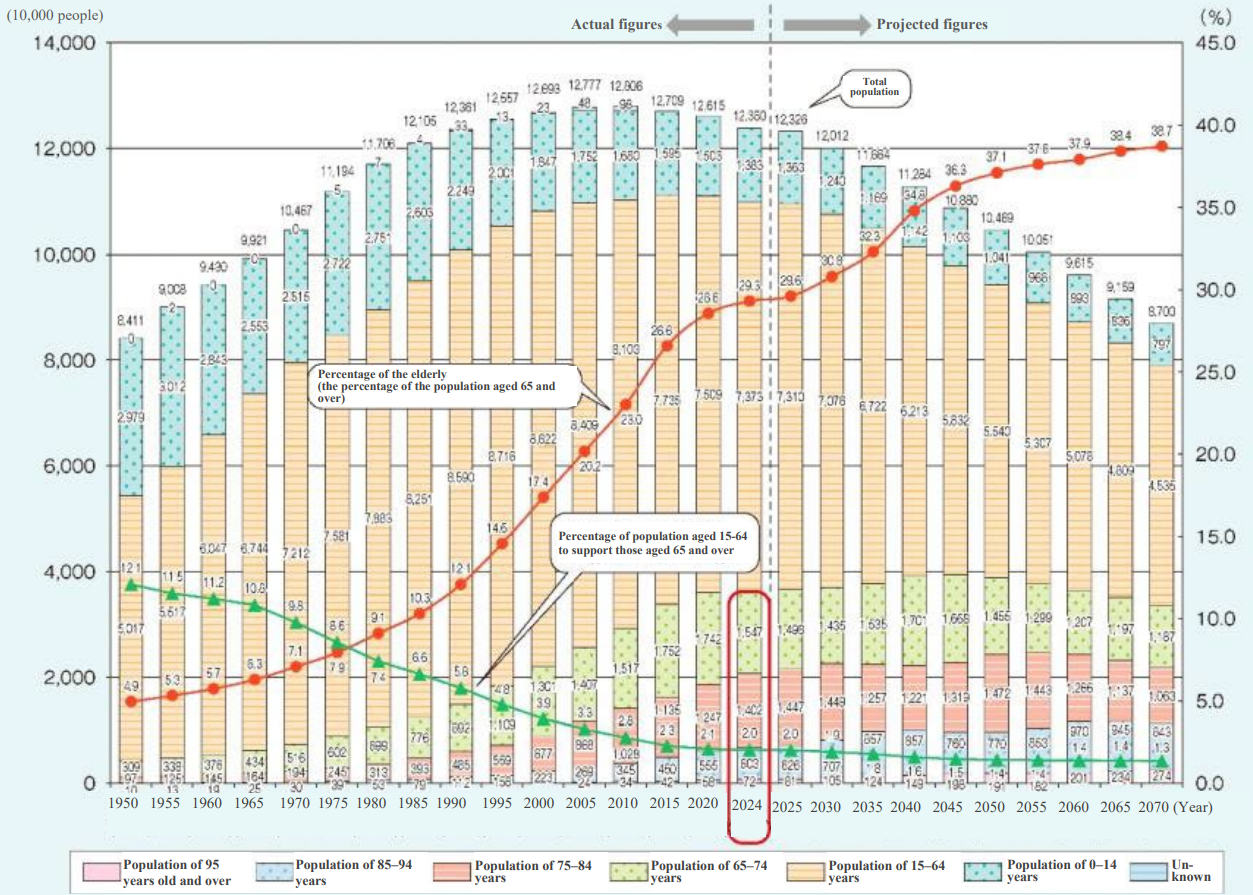
\includegraphics[width=0.75\linewidth]{fig/chp1/chp1_no_people.png}
    \caption{Trends in population ageing and future projections in japan\cite{cabinet_office_2025}}
    \label{fig:placeholder}
\end{figure}

この構造的な労働供給の縮小は，特に労働集約型産業である介護・家事支援サービス分野において顕著である．
厚生労働省の推計では，2040年度には約272万人の介護職員が必要となると予測されているが\cite{mhlw_caregiver_2024}，リクルートワークス研究所の報告によれば，現状のまま推移した場合，2040年には介護サービス職で約58万人の供給不足が生じると試算されている\cite{recruit_works_2024}．
このように増大し続ける支援需要と減少する労働供給の間の需給ギャップを埋めるため，ロボット技術による業務の代替・補完への期待はかつてないほど高まっており，サービスロボットの研究開発は喫緊の社会的要請となっている．

数ある家事支援の中でも，「料理（調理作業）」は特に重要性を持つ．
第一に，食事は生命維持と健康管理に直結する毎日数回の必須タスクであり，掃除や洗濯と比べて頻度が高い．
第二に，献立計画から食材の調達，下処理，加熱，配膳，後片付けに至るプロセスは，高度な身体的スキルと認知的負荷を同時に要求する．
特に高齢者にとって，刃物や火を扱う調理作業は身体機能の低下とともに危険を伴うようになり，自立生活を維持する上での最大の支障となりやすい．
したがって，単なる利便性向上を超え，介護と生活の質の維持の観点から，家庭内での調理を物理的に支援するロボットの実現が強く望まれている．

\subsection{産業用と家庭用ロボットの差異}

料理ロボットの研究開発は，その利用する場が「産業（工場）」か「家庭」かによって，求められる機能や設計思想が根本的に異なる．
食品工場などの産業現場では，調理プロセスの自動化が既に高度に進展しているが，これらは環境と対象物が厳密に管理された「構造化環境」を前提としている．

産業用ロボットのアプローチは「タスクの特化」にある．
例えば，ジュースの充填（液体），パン生地の混練（粘弾性体），魚の切り身の加工（柔軟物）など，ロボットにとって扱いが難しいとされる対象物であっても，工場ではそれぞれの作業に最適化された専用機械やライン（ベルトコンベアシステム等）を用いることで処理を実現している．
ここでは，単一の作業を大量に繰り返す「生産効率」が最優先され，そのために広いスペースや専用の大型設備を用いることが許容される．
つまり，産業用ロボットは，環境側をロボットに合わせて固定・管理することで，複雑な認識や適応的な制御を最小限に抑え，高効率な自動化を達成しているのである．

一方，一般家庭のキッチンで稼働するサービスロボットには，産業用とは対照的な「非構造化環境」への適応が求められる（表\ref{tab:robot_comparison}参照）．

% \begin{table}[ht]
%   \centering
%   \caption{産業用ロボットと家庭用ロボットの特徴と比較}
%   \label{tab:robot_comparison}
%   \begin{tabularx}{\textwidth}{@{}lXX@{}}
%     \toprule
%     比較項目 & 産業用ロボット（工場） & 家庭用ロボット（キッチン） \\
%     \midrule
%     \textbf{環境} & \textbf{構造化環境} \newline 照明・配置が厳密に管理・固定 & \textbf{非構造化環境} \newline 未知で動的に変化する実世界 \\
%     \midrule
%     \textbf{アプローチ} & \textbf{タスク特化} \newline 液体・粉末等は専用機械で処理 & \textbf{タスク汎用性} \newline 1台のロボットで全工程を処理 \\
%     \midrule
%     \textbf{対象物} & \textbf{性状を問わず，対象ごとに専用機構で取り扱う}  & \textbf{形状不定・柔軟物} \newline 個体差が大きく未知のものが多い \\
%     \midrule
%     \textbf{制約条件} & \textbf{大規模な専用スペース・設備が可能} & \textbf{人間と共存する限られた空間} \newline 省スペース性が必須 \\
%     \midrule
%     \textbf{優先指標} & \textbf{生産効率・速度} \newline 1秒間に何個処理できるか & \textbf{適応力・汎用性} \newline 未知の状況に対応できるか \\
%     \bottomrule
%   \end{tabularx}
% \end{table}
\begin{table}[ht]
  \centering
  \caption{Comparison between Industrial and Domestic Robots}
  \label{tab:robot_comparison}
  \begingroup
  \footnotesize
  \setlength{\tabcolsep}{4pt}
  \renewcommand{\arraystretch}{0.95}
  \begin{tabularx}{.95\textwidth}{@{}lXX@{}}
    \toprule
    Item & Industrial Robots & Domestic Robots \\
    \midrule
    \textbf{Environment}
    & \textbf{Structured} \newline Lighting and object placement are controlled
    & \textbf{Unstructured} \newline Conditions are unknown and dynamically changing \\
    \midrule
    \textbf{Approach}
    & \textbf{Task-specific} \newline Dedicated machines are used for each process
    & \textbf{Versatile} \newline A single robot handles multiple processes \\
    \midrule
    \textbf{Objects}
    & \textbf{Dedicated handling} \newline Objects are handled according to their properties
    & \textbf{Irregular and deformable} \newline Objects vary widely and are often unknown \\
    \midrule
    \textbf{Constraints}
    & \textbf{Dedicated space} \newline Large-scale equipment can be used
    & \textbf{Shared limited space} \newline Space-saving design is required \\
    \midrule
    \textbf{Priority}
    & \textbf{Efficiency and speed} \newline Processing quantity per unit time
    & \textbf{Adaptability} \newline Response to unknown situations \\
    \bottomrule
  \end{tabularx}
  \endgroup
\end{table}

\begin{enumerate}
    \item \textbf{スペースの制約：} 一般家庭には工場のような専用ラインや大型機械を設置する空間的余裕はないため，人間と共存できるサイズ（省スペース性）が必須となる．そのため，1台（あるいは双腕）のロボットアームとハンドを用いて，切るや炒める皮をむくといった，運動学的にも力学的にも性質の異なる多種多様な調理動作を，同一のハードウェアで遂行する能力が求められる．
    
    \item \textbf{対象物の不確実性と多様性：} 家庭内の食材は工業製品とは異なり，極めて高い「個体差」を持つ．同じ「ジャガイモ」であっても，その形状・大きさ・表面の凹凸・硬さは一つ一つ異なる個体差を持つ．また，調理器具や食器も規格化されておらず，未知の形状をした対象物を即座に認識し，適切に扱う能力が要求される．

    \item \textbf{道具・設備の非標準化（人間中心設計への適応）：} 工場ではロボット専用のハンドや治具が用いられるが，家庭では人間用に設計された既存の調理器具（包丁，ピーラー，鍋など）をそのまま利用しなければならない．ロボットは，自身の身体構造と関係なく作られた道具を把持し，その幾何学的・力学的機能を理解して操る能力が求められる．

    \item \textbf{センシング環境の悪条件：} 均一な照明が保証される工場とは異なり，家庭のキッチンでは，ステンレスの反射，水やガラスなどの透明物体，湯気による遮蔽など，視覚センサにとってのノイズ要因が極めて多い．不完全な点群データからでも，対象の物理モデルをロバストに再構成・推定する能力が必要となる．
\end{enumerate}


こうした困難な制約に対し，Miso RoboticsのFlippy\cite{miso2025flippy_nextgen}やMoley Roboticsのシステムなど，先駆的な取り組みが進められている．
しかし，これらの多くは依然として「専用設計された環境」や「規格化された手順」に依存している．
業務用のシステムは食材供給を固定化し，家庭用の既存システムも専用レシピや器具を前提とする場合が多い．
したがって，未知の食材や道具に対してその場で判断し適応する，真の意味での「非構造化環境への適応力」が，家庭用料理ロボット実現の鍵となる．

これらの家庭環境特有の課題は，ロボットによる物理的なマニピュレーションの観点から抽象化すると，本質的に（i）形状の多様性，（ii）力学的相互作用の複雑さ，（iii）環境・道具による拘束，という3つの「物理的制約」として整理できる．


\section{課題と提案手法}

\subsection{家庭環境での困難性}

前述の通り，家庭環境での適応性を実現するためには，調理作業に内在する以下の3つの物理的制約を克服する必要がある．

\begin{enumerate}
    \item \textbf{形状の多様性への適応（幾何学的不確実性）：} 食材の形状は不定形であり，事前に正確なモデルを用意することは不可能である．従来の剛体マニピュレーションで主流であった，既知のCADモデルとのマッチングに基づく姿勢推定や把持計画をそのまま適用することはできない．したがって，ロボットはセンサの点群情報から対象の局所的な表面曲率や法線ベクトルといった幾何特徴を即座に抽出し，個体差に合わせてオンラインで動作軌道を生成する能力が求められる．
    
    \item \textbf{複雑な力学的相互作用：} 調理は単なる物体の移動（ピックアンドプレース）ではなく，対象の物理的変形や状態変化を伴う．特に，包丁による「切断」やピーラーによる「皮むき」は，対象物の塑性変形や破壊を伴う不可逆なプロセスである．これらを成功させるためには，単なる位置制御ではなく，対象の硬さに応じた反力制御，皮むき時の接触圧維持など，実行時の接触状態に基づいた「力」の能動的な管理（インピーダンス制御等）が不可欠である．
    
    \item \textbf{環境・道具による拘束（ツール媒介操作の複雑性）：} ロボットは食材を直接操作するだけでなく，包丁，ピーラー，容器といった「道具（環境）」を介して間接的に作用させる．道具を使用する作業においては，ロボットのハンド，道具，対象物，そしてまな板の間に複雑な運動学的・力学的な拘束が生じる．道具が持つ幾何的な機能（例：容器の容積）や力学的な制約（例：刃が滑らない角度）を理解し，環境全体の物理モデルとして動作に反映させる必要がある．
\end{enumerate}

これらの困難性は，料理タスクが単なる視覚的なパターン認識や事前の軌道ティーチングだけでは解決できず，対象と環境に対する深い「物理的推論」を必要としていることを示している．
したがって，これらの物理的推論をロボットシステム上で実装可能な形で行うためには，実世界の対象と環境を，物理法則を適用できる「計算可能な内部表現」への落とし込むことが不可欠となる．

\subsection{提案手法：3Dモデルを基盤とした「分析主導型」アプローチ}

前節で述べた「形状・力・環境」という3つの物理的制約に対応するため，本研究ではRGB-Dセンサ等から得られる「3Dモデル」を物理世界の計算代理として構築し，それに対する多角的な「分析」を通じて適応的な「動作を生成する」統一的なアプローチ（図\ref{fig:topflow}）を提案する．

\begin{figure}[t]
    \centering
    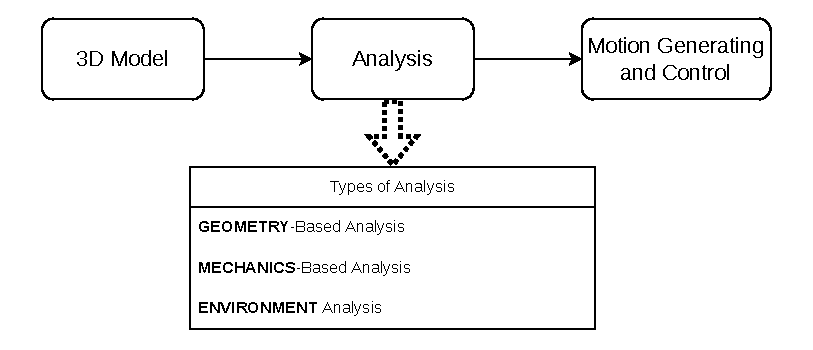
\includegraphics[width=.95\linewidth]{fig//chp1/DoctoralThesis_TopFlow.drawio.pdf}
    \caption{The flow of proposed approach}
    \label{fig:topflow}
\end{figure}

本研究において「3Dモデル」とは，主にRGB-Dセンサから取得された点群データを指し，必要に応じてメッシュ化や幾何プリミティブへのフィッティング処理が施されたものを意味する．
このモデルに対し，以下の3つの観点から分析を行うことで，前述の課題を解決する．

\begin{enumerate}
    \item \textbf{幾何学的な分析：} 対象物の3D形状（法線，体積など）を解析し，その形状的特徴に合わせてロボットの軌道を生成する．これは「形状の多様性」への直接的な解となる．
    
    \item \textbf{力学的な分析：} 3Dモデル上で，切断時の反力，摩擦，モーメントの釣り合いを解析・シミュレーションする．これにより「複雑な力学的相互作用」における動的な安定性を実現する．
    
    \item \textbf{環境的な分析：} 食材単体ではなく，容器や刃物といった「環境（道具）」との幾何的・力学的関係性を解析する．これにより「環境・道具による拘束」を考慮した間接的な操作が可能となる．
\end{enumerate}

また，本アプローチでは，分析によって導出された動作計画を基本とし，必要に応じて力覚センサ等を用いたフィードバック制御を併用する．
すなわち，3Dモデル上の分析が大まかな「解」を与え，実世界での接触情報が微細な誤差を吸収するという階層的な構造をとることで，ロバストなタスク遂行を保証する．

本論文が提案するのは，あくまで「3Dモデル上の分析から動作パラメータを導出する」という設計アプローチであり，あらゆる料理タスクを全自動化する単一のシステムではない．
しかし，このアプローチは多様な物理的制約を持つタスクに対して汎用的に適用可能である．

\section{目的と検証タスクの選定}

\subsection{本論文の目的}

% 本論文の目的は，RGB-D点群から構築した3Dモデルにより作業環境および対象物を表現し，その幾何・物理的特徴に基づく推論を通じて，動作と制御の設計を行う汎化可能な操作設計のアプローチを提示することにある．
% 具体的には，未知の食材や道具に対しても，その場で取得した3Dモデルに対する物理的な整合性の分析を行うことで，適応的な行動則を導出できることを示す．
本論文の目的は，RGB-D点群から構築した3Dモデルを計算基盤として，対象物および作業環境の幾何・物理的特徴を分析し，その結果をタスク固有の動作生成および制御設計へ接続する操作設計アプローチを提示することにある．
さらに，物理的相互作用の性質が異なる複数の料理操作に本アプローチを適用し，その有効性と適用可能性を検証する．
具体的には，形状が事前に与えられていない（以降は「未知」とよぶ）食材や道具に対しても，その場で取得した3Dモデルの幾何・物理的な特徴を分析することにより，対象に適応したロボットの動作生成および制御設計が可能であることを示す．

\subsection{検証タスクの選定}

提案する「分析主導型」アプローチの有効性を実証するため，本論文では物理的相互作用の特性が大きく異なる以下の3つのタスクを選定した．
これらは，料理作業における代表的な物理対象（流体・固形食材・道具）を含み，さらに状態変化（不可逆変形・破壊）と接触/環境制約を主要な観点としてカバーするように設計した．

% \begin{table}[htbp]
%   \centering
%   \caption{検証タスクと適用される分析手法の対応}
%   \label{tab:tasks}
%   \begin{tabular}{@{}cccc@{}}
%     \toprule
%     検証タスク & 1. 幾何学的な分析 & 2. 力学的な分析 & 3. 環境的な分析 \\
%     \midrule
%     \textbf{タスク1：皮むき} &  法線・軌道 & 実行中接触圧維持 & ------ \\
%     \addlinespace
%     \textbf{タスク2：注ぐ} &  容積・形状 & ------ &  容器間関係 \\
%     \addlinespace
%     \textbf{タスク3：安定把持} &  把持点探索 &  力学解析 &  道具拘束 \\
%     \bottomrule
%   \end{tabular}
% \end{table}
\begin{table}[htbp]
  \centering
  \caption{Correspondence between validation tasks and applied types of analysis}
  \label{tab:tasks}
  
  \scriptsize
  \setlength{\tabcolsep}{4pt}
  \renewcommand{\arraystretch}{0.95}
  \begin{tabularx}{.95\textwidth}{@{}cccc@{}}
    \toprule
    Validation Task & 1. Geometric Analysis & 2. Mechanics-Based Analysis & 3. Environmental Analysis \\
    \midrule
    \textbf{1st: Peeling} & Surface Normals and Trajectory & Contact Pressure Maintenance & ------ \\
    \addlinespace
    \textbf{2nd: Pouring} & Volume and Shape & ------ & Inter-Container Relationship \\
    \addlinespace
    \textbf{3rd: Holding} & Holding Point Search & Mechanics-Based Evaluation & Tool Constraints \\
    \bottomrule
  \end{tabularx}
\end{table}

\begin{enumerate}
    \item \textbf{タスク1：皮むき動作（不規則形状への幾何的適応と接触維持）} \\
    このタスクは，個体差の大きい「不規則な曲面形状」への適応能力を検証する．3Dモデルを用いた\textbf{「幾何学的な分析」}により最適な刃の軌道を生成し，実行時の力制御でモデル誤差を吸収することで，形状の不確実性に対応できることを示す．
    
    \item \textbf{タスク2：注ぎ動作（容器という「環境」を利用した流体操作）} \\
    このタスクは，直接把持できない「流体」の操作能力を検証する．対象物そのものではなく，容器の3Dモデルに対する\textbf{「環境的な分析」}（容積推定や流出特性の解析）と\textbf{「幾何学的な分析」}を行うことで，外部計量器具なしに定量的な操作が可能であることを示す．
    
    \item \textbf{タスク3：安定把持（外力に抗する力学的・環境的推論）} \\
    このタスクは，切断という「大きな外力」および包丁という「道具」が存在する状況下での高度な推論能力を検証する．3Dモデル上で想定される切断力や摩擦力をシミュレーションする\textbf{「力学的な分析」}と，包丁やまな板との関係を考慮する\textbf{「環境的な分析」}を統合し，最適な把持戦略を導出できることを示す．
\end{enumerate}

\subsection{本論文の寄与}

本論文の主な寄与は，アプローチの提案，タスク固有アルゴリズムの開発，および実ロボットシステムでの実証という観点から，以下の3点に要約される．

\begin{enumerate}

\item \textbf{アプローチの確立（3Dモデルベースの分析主導型設計）} \\
非構造化環境における料理タスク群に対し，RGB-D点群から構築した3Dモデルを物理世界の「計算代理」と位置づけ，そこでの幾何学的・力学的・環境的な分析を通じて適応的な動作と制御パラメータを導出する「分析主導型」の操作設計アプローチを提案した．これにより，従来多く用いられてきた発見的ルールや事前ティーチングに依存する方法に対し，物理法則に基づく動作設計のための体系的な設計指針を与える．

\item \textbf{具体的アルゴリズムの開発（料理操作における代表的物理相互作用への適用）} \\
提案する設計手法を，物理的特性が大きく異なる3つの料理タスク（皮むき，注ぐ，切断把持）に適用し，それぞれのタスクを解決するための具体的なアルゴリズムを開発した．具体的には，(a) 不規則形状の食材に対する幾何学的軌道生成と力覚制御を統合した皮むき手法，(b) 未知容器の3D幾何および環境推論に基づく定量注液手法，(c) 包丁からの外力と環境拘束を考慮した力学解析による安定把持点探索手法を提案した．

\item \textbf{実機実験による検証（実ロボットによる未知対象操作の検証）} \\
開発した手法を双腕ロボットシステムに実装し，事前の精密なCADモデルを与えられていない未知の食材や容器に対しても提案手法が適用可能であることを実験により確認した．

\end{enumerate}

\section{本論文の構成}


本論文は全7章で構成される．
第2章では，調理ロボットに関連する先行研究を概観する．
産業用ロボットのアプローチと，家庭用ロボットに求められる非構造化環境への適応に関する研究動向を整理し，本研究の立ち位置を明確にする．
第3章では，本研究の基礎となる3Dモデルの取得手法，および実験プラットフォームの構築について述べる．
RGB-Dセンサを用いた点群取得，前処理，モデル化のプロセスと，その精度検証について詳述する．
第4章では，「皮むく」タスクを通じ，3Dモデルの表面幾何解析による軌道生成と力覚フィードバックの統合手法について論じ，その有効性を検証する．
第5章では，「注ぐ」タスクを通じ，容器の3Dモデルを用いた幾何学的推論（容積計算）に基づく流体操作手法について論じ，その有効性を検証する．
第6章では，「安定把持」タスクを通じ，包丁からの外力に対する力学解析と環境解析を統合した把持計画手法について論じ，その有効性を検証する．
最後に第7章において，本論文を総括し，今後の展望を述べる．
以上の構成により，第3章で三つのタスクに共通する計測・モデリング基盤を示し，第4章から第6章で，皮むき，定量注ぎ，および切断中の安定把持という三つの研究課題を順に検証する．
各検証章では，第1章で示した「3Dモデル，分析，動作計画・制御」の関係を同一の観点から整理し，最終章で得られた知見と適用範囲を総括する．





	\chapter{関連研究}
\revise{本章では，家庭用料理ロボットの操作実行層における本研究の位置づけを明確にするため，先行研究を形状，力学，環境・道具という三つの分析観点と，三つの検証タスクから整理する．まず，料理ロボット全体の研究動向を概観し，レシピ理解やタスク計画と，それらが決定された後の物理操作実行との境界を確認する．次に，各分析観点に関する研究を整理し，最後に皮むき，定量注ぎ，および切断中の安定把持に関連する研究と本論文のタスク固有手法を比較する．}

\section{料理ロボットの研究}
料理ロボットに求められる汎化能力と物理的相互作用の観点について，Sochackiら\cite{Sochacki2024PracticalChefReview}は料理ロボットに関する包括的なレビューを行い，家庭環境での調理では対象物の状態変動と複雑な接触相互作用が支配的であり，単純なピックアンドプレースだけではタスクが成立しないことを指摘している．

調理タスクにおける道具媒介操作と計画の観点では，家庭環境の複雑さに対応するため，Bolliniら\cite{Bollini2013RecipesCookingRobot}やZhangら\cite{Zhang2024RealWorldCookingFromRecipes}は，自然言語のレシピ指示からロボットの行動計画を生成し，統合システム上で実行するアプローチを提案している．
また，Kümpelら\cite{Kumpel2025CookingActions}は調理タスクを特定の操作カテゴリに写像するための知識表現を提案し，Beetzら\cite{Beetz2011CRAM}やPauliusら\cite{PauliusSun2019CookingSurvey}は認知ロボットアーキテクチャや知識表現に基づく計画の重要性を論じている．
さらに，Beckerら\cite{Becker2011KitchenContainers}はキッチン環境でのモバイルマニピュレーションを実装した．
\revise{これらの研究はタスクレベルの計画や論理表現を主眼とするため，計画された個々の操作について，対象物の個体形状や接触条件から軌道，操作量，把持位置，力などを決定する実行層の問題は，別途解く必要がある．}
また近年，Welteら\cite{Welte2025DexterousILSurvey}やWangら\cite{Wang2025EmbodiedVisualPerceptionSurvey}がレビューするように，模倣学習やエンボディドAIに基づく視覚と操作の統合も盛んである．
しかし，料理における道具を介した操作には厳密な物理制約が存在する．
\revise{本論文は，操作目的，使用する道具，および基本条件が決定された後の「動作と制御パラメータの導出」に焦点を当てる．3Dモデルはそのための入力表現であり，形状だけでなく，タスクごとに既知または計測可能な物理条件と組み合わせて用いる．}

\section{幾何学的な分析に基づく操作設計}
家庭環境の多様な形状に適応するための3Dモデル化と環境認識について，ロボットビジョンにおける3D再構成技術は，RGB-Dセンサの発展とともに成熟してきた．
Newcombeら\cite{Newcombe2011KinectFusion}が提案したKinectFusionは，TSDF（Truncated Signed Distance Function）を用いてリアルタイムな密3D再構成を実現した古典的かつ強力な手法である．
その後，Whelanら\cite{Whelan2015ElasticFusion}によるElasticFusionやDaiら\cite{Dai2017BundleFusion}によるBundleFusionにより，非剛体整合やグローバル整合の最適化が進展した．
また，近年の屋内3Dモデリングの動向\cite{Yuan2021RGBDIndoorSurvey}や，計算効率を高めたTSDF融合手法\cite{Li2024RGBTSDF}，さらにはGaussian Splattingを用いたオンラインマッピング\cite{GSFusion2024}やNeRFとRGB-Dを組み合わせた表面再構成\cite{Lee2024InFusionSurf}など，より高品質なモデル化手法が提案されている．
これらの技術は，本研究が前提とする「計算代理としての3Dモデル」を構築するための不可欠な基盤となる．

幾何特徴抽出と軌道生成に関して，取得した点群から，法線や曲率などの幾何特徴を抽出することは，操作設計の第一歩である．
NguyenとLe\cite{Nguyen2013PointCloudSegSurvey}は点群セグメンテーションの包括的なサーベイを提供し，Martínez-Otzetaら\cite{MartinezOtzeta2022RANSACSurvey}はRANSACを用いた平面やモデルの推定の有用性を整理した．
さらに，これらの幾何情報を直接利用した軌道生成として，Yuら\cite{Yu2021PointCloudSlicingRobotica}やZhangら\cite{Zhang2025ContourParallelToolpathPointCloud}は，点群をスライスして断面輪郭を抽出し，ツールパスを生成するアルゴリズムを提案している．
Zengら\cite{Zeng2024ShapeFollowingLaserCleaning}も3D点群表面に基づく形状追跡軌道の計画を行っている．
本論文における「皮むき」タスクの軌道設計は，これらの断面抽出アプローチと軌を一つにするが，さらに力学的接触の維持を統合する点に特徴がある．

\section{力学的な分析に基づく操作設計}
調理操作における対象物の変形や破壊を伴う接触タスクと基本制御について，ロボットが環境と接触する際の制御理論として，Hogan\cite{Hogan1985ImpedanceControl}のインピーダンス制御や，RaibertとCraig\cite{RaibertCraig1981Hybrid}のハイブリッド位置/力制御が広く知られている．
これらの古典的枠組みは，拘束方向と自由方向を分離・管理する上で現在も極めて有効である．

外力が加わる状況下の安定性解析と外乱耐性に関して，切断や保持において外力が加わる場合，把持の安定性評価が必要不可欠である．
Bicchi\cite{Bicchi1995Closure}は力学的なClosure特性を統一的に論じ，FerrariとCanny\cite{FerrariCanny1992OptimalGrasps}はWrench空間に基づく把持の品質指標（Grasp quality measures）を提案した．
RoaとSuárez\cite{RoaSuarez2014GraspQualityReview}はこれらの指標を総括し，外乱に対する抵抗力がタスクの成否を分けることを示している．
本論文の「安定把持」タスクは，まさに切断反力を抵抗する適切な把持点の探索問題である．

食品の切断モデルと把持の近年方向について，食品切断の力学は非常に複雑である．
Mitsioniら\cite{Mitsioni2021FoodCuttingDynamics}は切断ダイナミクスをRNNで学習し制御に組み込んだ．
Muら\cite{Mu2019RoboticCutting}やJamdagniら\cite{Jamdagni2019FractureMechanicsCutting}は，破壊力学に基づき切断過程の摩擦と破断力をモデル化している．
また，Zhouら\cite{Zhou2006PressingSlicingCutting_1, Zhou2006PressingSlicingCutting_2}は，押し込みとスライスを組み合わせた生体材料の切断メカニズムを分析した．
一方，近年の把持研究においては，Songら\cite{Song2025DexterousGraspingOverview}が学習ベースの把持を総覧し，Srinivasら\cite{Srinivas2025GraspFactory}は外乱下での把持ロバスト性を考慮したデータセットを構築している．
本論文は，これらの切断力学モデルを外力として取り込み，把持品質の解析的評価関数に組み込むことで，安定した切断中の把持を実現する．

\section{環境分析に基づく操作設計}
環境拘束の積極的な利用とタスク・モーションプランニングに関して，Garrettら\cite{Garrett2021TAMPSurvey}やZhaoら\cite{Zhao2024OptTAMPSurvey}のレビューが示す通り，離散タスクと連続運動の統合計画において，幾何的制約と衝突回避は中核的な課題である．
Stilman\cite{Stilman2011ConstrainedManipulation}は環境拘束下での操作計画を定式化し，Görnerら\cite{Gorner2019MoveItTaskConstructor}はこれらを実装可能なフレームワークとして提供している．
さらに，Nakatsuruら\cite{Nakatsuru2023EnvironmentSupport}は，壁や机などの環境支持を積極的に利用する計画手法を提案し，
Ard{\'o}nら\cite{Ardon2021AffordanceReview}も環境と対象の相互作用可能性を表現するアフォーダンス関係の学習・表現についても，設計選択と汎化の観点から体系的な整理が進められている．

不確実性の高いキッチン環境における能動知覚と環境モデリングについて，Bohgら\cite{Bohg2016InteractivePerception}が提唱するインタラクティブ知覚のように，ロボット自身の行動を通じて観測を改善するアプローチが重要となる．
本論文におけるモデルの計測方針は，対象周囲の複数視点からの点群取得に加え，必要に応じて対象を把持して底面側を観測し，取得した点群を統合することで不完全観測を低減するという実践的なアプローチとして位置づけられる．

\section{タスクごとの先行研究}
本節では，本論文で検証タスクとして取り上げる「注ぐ」「皮むき」「安定把持」の各操作に関する個別研究を整理し，提案手法の有効性を明らかにする．

\subsection{皮むきに関する研究}
皮むき動作は，不規則な曲面に対する幾何学的な軌道追跡と，接触力を維持する力制御の統合が必要なタスクである．
Houら\cite{Hou2022PeelingPlanning}は自動皮むきのための幾何的な経路設計問題を整理した．
また，マルチモダルな情報とインピーダンス制御を用いた単腕皮むきシステム\cite{Arxiv2024MultimodalPeeling}や，対象物の再配向を伴う拘束付き巧緻操作としての皮むき\cite{Arxiv2024ConstrainedDexterousPeeling}も実機実装として報告されている．

剥皮を成立させる前提となる手内操作（In-hand manipulation）能力については，Rojasら\cite{Rojas2016GR2}の劣駆動機構による手内平面操作，Maら\cite{Ma2017WholeHandCaging}のCagingによるロバスト把持，McCannとDollar\cite{McCann2017StewartHand}のパラレルメカニズム型ハンド，Mnyusiwallaら\cite{Mnyusiwalla2016BioInspiredInsideHand}の生体模倣指などが提案されている．
さらにLiarokapisとDollarは，手内操作のプリミティブ抽出\cite{Liarokapis2017Primitives}やタスク特化モデルの学習\cite{Liarokapis2016TaskSpecificModels}を論じている．
微小力センシングの観点では，網膜手術などの医療分野における微小力フィードバック研究\cite{Balicki2010MicroForcePeeling}が，接触力管理の設計思想として参考になる．
\revise{本論文の皮むき操作は，食材ごとの形状から到達可能な軌道を生成し，表面法線に基づく領域分割と既処理境界に基づく食材回転を行い，さらに力覚フィードバックで点群誤差と表面凹凸を補償する点に特徴がある．}

\subsection{注ぐに関する研究}
ロボットによる注ぎ操作は，液体モデルの複雑さと容器の多様性から多くの研究がなされてきた．
Rozoら\cite{Rozo2013PouringForceBased}は力覚に基づく模倣学習を，Chenら\cite{Chen2019RNNMPCPouring}はRNNとMPCを組み合わせた注ぎ制御を提案した．
また，López-Guevaraら\cite{LopezGuevara2017NotToSpill}は近似流体モデルを用いた強化学習を行い，衝突回避を含めた注ぎの動作計画\cite{AAAI2023PouringPlanning}も提案されている．
Reyes-Montiel\cite{ReyesMontiel2026PouringReview}の最新のレビューやHuangら\cite{Huang2021SelfSupervisedPouring}の自己教師あり学習の事例は，流体操作における学習ベース手法の隆盛を示している．

一方，解析的なアプローチとして，DoとBurgard\cite{DoBurgard2018AccuratePouring}やSchenckとFox\cite{SchenckFox2017ClosedLoopPouring}，Kennedyら\cite{Kennedy2017Dispensing}は，RGB-Dカメラや視覚フィードバックを用いた高精度な閉ループ制御を報告している．
容器の幾何形状に着目した研究としては，Brandlら\cite{Brandl2014WarpedPouring}のワーピングによる一般化や，Mottaghiら\cite{Mottaghi2017GlassHalfFull}の画像からの容積推定がある．
液面知覚に関しては，ステレオ視による流動観測\cite{YamaguchiAtkeson2016StereoFlow}，深層学習による液体知覚\cite{SchenckFox2016LiquidsISER}，RGB-Dを用いた確率的液面推定\cite{Do2016ProbLiquidLevel}などが提案されており，失敗からの回復を学習に組み込む試み\cite{Langsfeld2014FailureToSuccessPouring}も存在する．
\revise{本論文の注ぎ操作は，事前登録した容器形状や制御用の外部計量器具に依存せず，対象容器の3D点群から液面高さと体積の関係，または容器角度と流出量の関係を導出し，指定量に対応する制御目標へ変換する点に特徴がある．}

\subsection{切断時の安定把持に関する研究}
切断における把持安定化の研究は，切断自体の制御と把持計画の融合領域に位置する．
切断制御の古典としてZengとHemami\cite{ZengHemami1997Cutting}やJungとHsia\cite{JungHsia1999Cutting}による適応制御があり，近年では視覚ベース切断の課題整理\cite{Singh2025VisionBasedCuttingSurvey}や，前述の学習動力学\cite{Mitsioni2021FoodCuttingDynamics}が提案されている．
切断力学に基づく刃物の運動最適化については，MuとJia\cite{MuJia2022PropertyKnifeOpt}の物性推定や，Zhouらの詳細な応力分布・力学モデル\cite{Zhou2006PressSliceI, Zhou2006PressSliceII}，Atkinsら\cite{Atkins2004CheddarSalami}の柔軟材料における押し引き切断の分析が重要である．
視覚と力覚を統合した柔軟物切断制御\cite{Long2014ForceVisionCutting}も存在する．

外力に対する安定把持計画の基礎としては，Millerら\cite{Miller2003ShapePrimitives}の形状プリミティブ近似，MirtichとCanny\cite{MirtichCanny1994OptGrasps}の実用的最適把持計算，Pelossofら\cite{Pelossof2004SVMGrasping}のSVMを用いた学習把持，Nguyen\cite{Nguyen1988ForceClosure}のForce-Closureの幾何的構成法が挙げられる．
多指ハンドにおける力の分離については，YoshikawaとNagai\cite{YoshikawaNagai1987Forces}の操作力と把持力の概念や，Donnerら\cite{Donner2018WrenchDecomposition}の物理的に妥当なWrench分解手法が強力な理論的背景となる．
さらに，拘束環境下での衝突を考慮した把持\cite{Lou2021CollisionAwareGrasping}や，重心と力覚に基づく姿勢適応\cite{Kanoulas2018CoMGraspAdapt}など，環境制約と外乱を同時に扱う技術が進展している．
\revise{本論文では，形状から衝突しない把持点を選ぶだけでなく，既知の包丁軌道に沿って時間変化する切断Wrenchを推定し，摩擦および力・モーメントの釣合いとともに把持安定性評価へ組み込む点に特徴がある．}

\section{まとめ}
以上の関連研究は，大きく次の三つのアプローチとして整理できる．
第一に，RGB-D等のセンシングに基づく3Dモデリングと幾何学的解析を基盤とし，対象形状の推定や表面特徴量の抽出を通じて，軌道生成や作業パラメータの導出へ接続する方向性である
\cite{Yuan2021RGBDIndoorSurvey,Li2024RGBTSDF,GSFusion2024,Lee2024InFusionSurf,Nguyen2013PointCloudSegSurvey,MartinezOtzeta2022RANSACSurvey,Yu2021PointCloudSlicingRobotica,Zhang2025ContourParallelToolpathPointCloud,Zeng2024ShapeFollowingLaserCleaning}．
第二に，接触を伴う操作を安定化するための力制御・インピーダンス制御，および切断や把持に関する力学モデル・評価指標を整備し，外力や接触状態の変動に対してロバストな実行を目指す方向性である
\cite{Hogan1985ImpedanceControl,RaibertCraig1981Hybrid,Bicchi1995Closure,FerrariCanny1992OptimalGrasps,RoaSuarez2014GraspQualityReview,Mu2019RoboticCutting,Jamdagni2019FractureMechanicsCutting,Zhou2006PressingSlicingCutting,Long2014ForceVisionCutting,Mitsioni2021FoodCuttingDynamics,MuJia2022PropertyKnifeOpt}．
第三に，道具や作業台を含む環境との相互作用を前提とし，拘束条件の明示化，能動的な再計測，および相互作用可能性（アフォーダンス）の表現を通じて，ツール媒介操作を成立させる方向性である
\cite{Bohg2016InteractivePerception,Ardon2021AffordanceReview,Stilman2011ConstrainedManipulation,Nakatsuru2023EnvironmentSupport,Mottaghi2017GlassHalfFull}．

\begin{revisionblock}
これらの研究により，形状認識，接触制御，環境利用に関する知見はそれぞれ蓄積されてきた．
一方，皮むき，注ぎ，切断中の把持では，3Dモデルから求める量も，最終的な動作・制御パラメータも異なるため，一般的な「計測，分析，動作生成」の流れだけでは各操作は成立しない．
本論文の位置づけは，形状，力学，環境・道具という共通の観点で相補的な事例を選び，皮むきでは表面追従と力制御，注ぎでは容器幾何と操作量，安定把持では切断Wrenchと接触力という，タスク固有の対応関係を構成して実機で検証する点にある．
次章では，これらに共通して必要となるロボットシステムとRGB-D点群の取得・処理・評価方法を示す．
\end{revisionblock}









	\chapter{システム構成と3Dモデルの取得}
\label{ch:system}

本章では，本論文で扱う三つの料理マニピュレーション研究に共通する基盤として，ロボットシステムの構成と，対象物および作業環境の3Dモデル取得方法を述べる．
以下では，第1章の3Dモデルのうち，主に点群表現を用いるため，3D点群モデルまたは点群モデルと呼ぶ．
\revise{本章で扱う3Dモデルは，三つのタスクに共通する計測表現である．ただし，その取得処理自体を単一の操作アルゴリズムとはみなさず，各タスクでは点群から異なる量を抽出し，固有の動作生成，力学解析，または制御設計へ用いる．}
このため，各タスク実現するための詳細なアルゴリズムを述べる前に，それらの前提となる共通の計測・モデリング過程を明確にしておく必要がある．

本論文で扱うタスクは，皮むき作業，液体を注ぐ作業，および切断時の安定把持である．
これらは対象物の物理特性や要求される制御方式こそ異なるものの，いずれも対象物の三次元形状や作業空間の幾何情報を把握し，そこから操作に必要な量を計算するという点で共通している．
具体的には，注ぐ操作では容器内部形状から容積や液面検出に必要な情報を得る必要があり，皮むき操作では食材表面形状から軌道を生成する必要があり，切断する時の把持では食材表面上で把持点候補を生成し，把持安定性を評価する必要がある．

% なお，システムの一部（ロボットアーム，ソフトウェアフレームワーク）は研究の進行に伴い変更が生じたが，3Dモデル取得・処理のアルゴリズムは全研究で一貫しており，本章後半で述べる点群処理パイプラインは制御方式には依存しない共通基盤として位置づけられる．

このような観点から，本章ではまず各研究で用いたロボットシステムを整理し，次にRGB-Dカメラを用いた多視点撮影による3Dモデル生成手順を述べる．
さらに，生成した3Dモデルから抽出される幾何情報と，各タスクにおけるその利用方法をまとめる．
最後に，3Dモデル取得の精度評価について述べ，本章で構築する基盤の妥当性を示す．

\section{システム構成：ハードウェア}
\label{sec:system:hardware}

本研究では，料理マニピュレーションの実装と評価に用いる実験プラットフォームとして，二種類の双腕ロボットシステムを構成した．
一つは，三菱重工製PA10-7Cを二台用いた双腕ロボットシステムであり，注ぐ動作，皮むき動作，および安定把持の検証に用いた．
もう一つは，DENSO製VS-050を二台用いた双腕ロボットシステムであり，安定把持の実機検証に用いた．
いずれのシステムにおいても，RGB-Dカメラ，力覚センサ，タスク固有のエンドエフェクタを組み合わせ，対象物の3Dモデル取得とロボット動作生成を行う構成とした．

本節では，まず各プラットフォームのロボットアーム構成を述べ，続いて力覚センサ，視覚センサ，座標系定義，カメラキャリブレーション，およびエンドエフェクタ設計について説明する．

\begin{revisionblock}
\subsection{ハードウェア設計方針}
本研究のハードウェアは，対象物を操作する機能と，操作に必要な形状・接触情報を計測する機能とが相互に妨げないことを方針として設計した．
具体的には，双腕構成により対象物・道具の保持と操作を分担し，交換可能なエンドエフェクタによりピーラー，容器，包丁，食材への接触機能を与えた．
さらに，手首力覚センサを道具とアームの間に配置して接触力を直接計測し，RGB-Dカメラを手先側に配置して視点を能動的に変更できるようにした．

エンドエフェクタについては，道具を確実に固定する側では剛性と再現性を優先し，食材へ接触する側では指先を小さな点接触として扱える形状と到達長を優先した．
カメラと指の配置は，指先が対象表面へ到達できることに加え，計測時の自己遮蔽を抑え，必要に応じて対象を持ち上げたまま下面を観測できることを条件とした．
この設計により，操作用機構を追加しても3D計測領域をできるだけ維持し，計測と操作を同じシステム内で反復できる．
なお，本章の装置は手法検証用の実験プラットフォームであり，寸法や設置形態をそのまま家庭へ導入することを意図したものではない．
\end{revisionblock}


\subsection{ロボットシステム}
\label{sec:system:hardware:robot-system}

\paragraph{PA10-7Cを用いた双腕ロボットシステム}

\begin{figure}[ht]
    \centering
    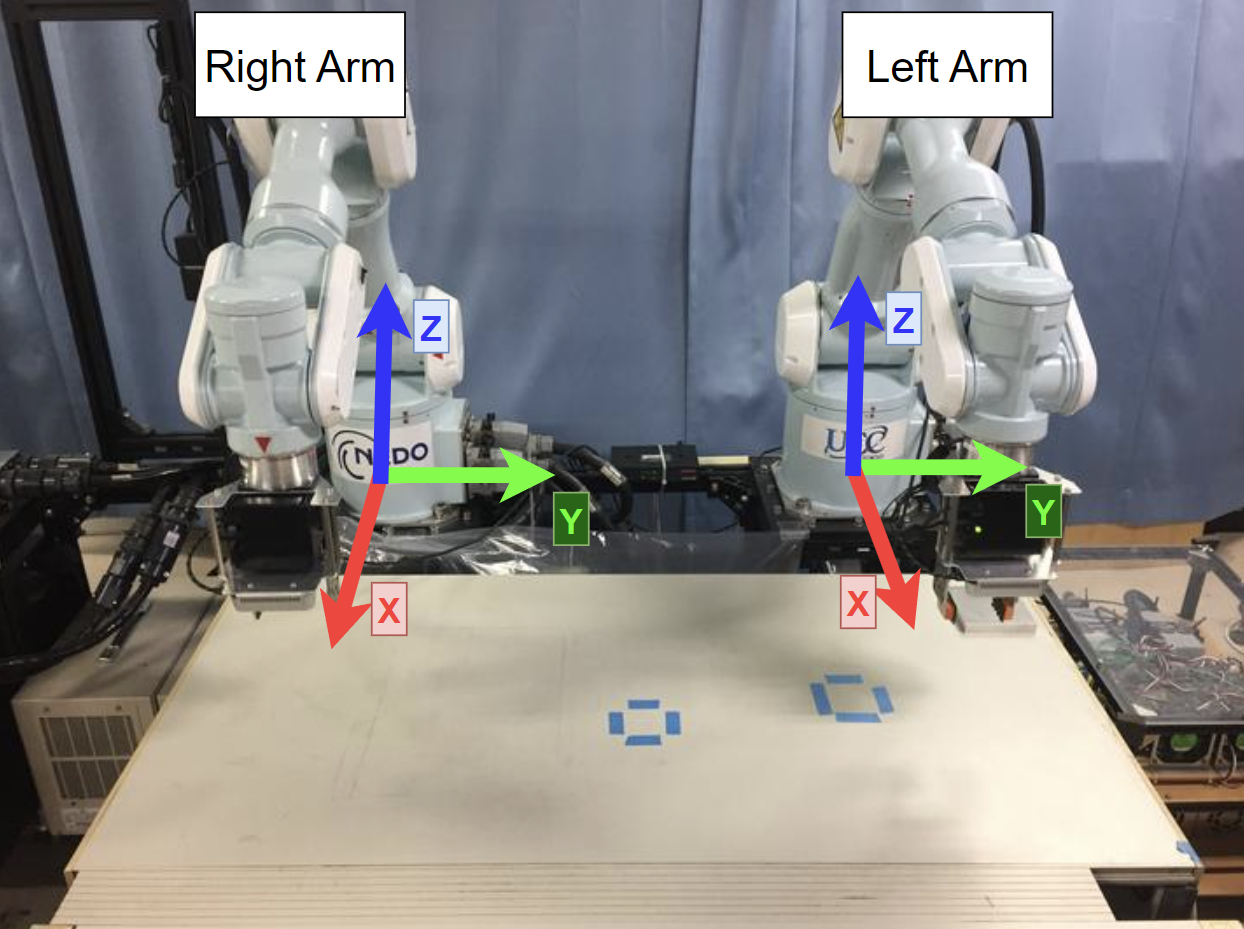
\includegraphics[width=0.8\linewidth]{fig/chp3/chp3_old_robot_coordinate.drawio.png}
    \caption{The coordinate system of PA10-7C.}
    \label{fig:system:robot-env-pa10}
\end{figure}

PA10-7Cを用いたロボットシステムでは，三菱重工製の7自由度マニピュレータPA10-7Cを2台用いた（図\ref{fig:system:robot-env-pa10}）．
両アームは卓上作業に適するよう床面から約700\,mmの高さに設置し，各アームのベース座標系の原点は各アームの底の中央に設定した．
この構成では，左右のアームを独立に制御しながら，片腕で対象物または道具を保持し，他方の腕で操作を実行する双腕協調作業を行う．

\paragraph{DENSO VS-050を用いた双腕ロボットシステム}

\begin{figure}[ht]
    \centering
    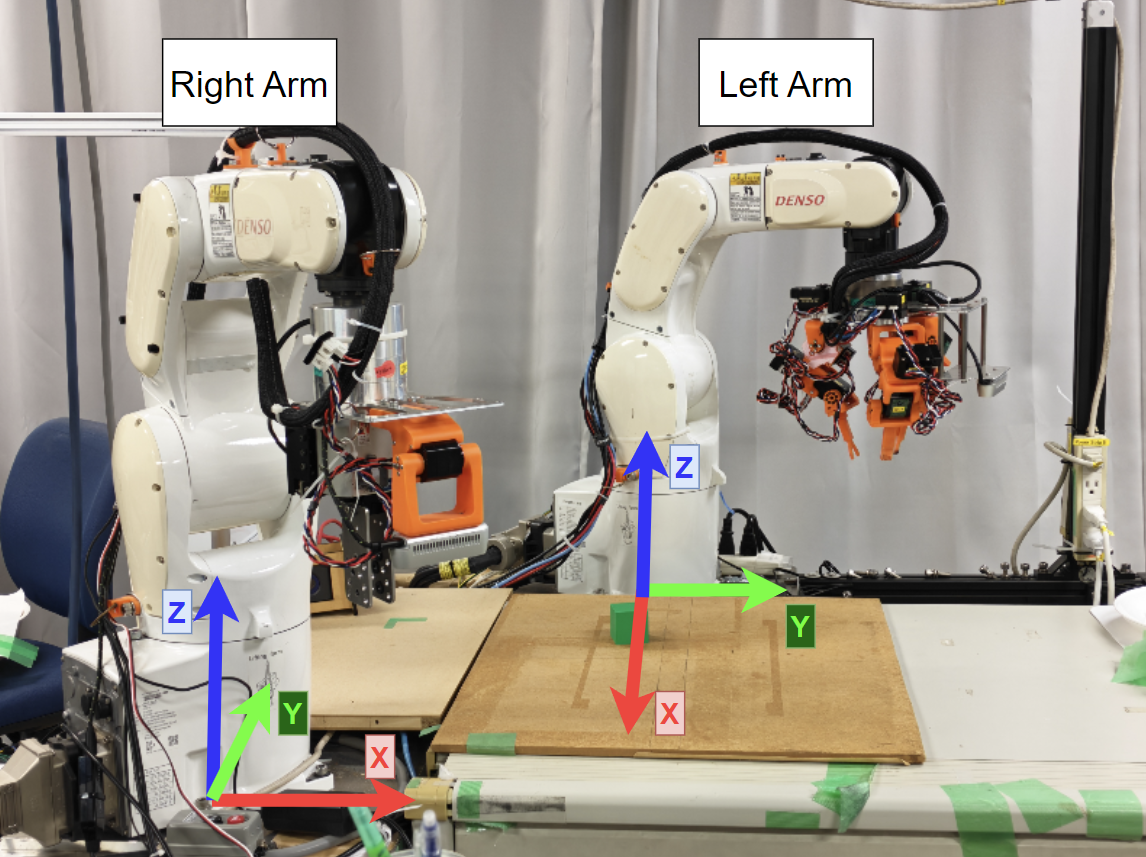
\includegraphics[width=0.8\linewidth]{fig/chp3/chp3_new_robot_coordinate.drawio.png}
    \caption{The coordinate system of DENSO VS-050.}
    \label{fig:system:robot-env-denso}
\end{figure}

DENSO VS-050を用いたロボットシステムでは，6軸の多関節ロボットVS-050を2台用いた（図\ref{fig:system:robot-env-denso}）．
VS-050は可搬質量4\,kg，位置繰り返し精度$\pm 0.02$\,mmの性能を有する．
本研究ではPA10-7Cの場合と同様に双腕構成として使用し，手先フランジ中心を基準としたツール座標系を定義した．
また，世界座標系は左アームのベース座標系に設定し，右アームで取得・計算される点群および操作点も同一の世界座標系上で扱えるようにした．

PA10-7CとDENSO VS-050では，アームの自由度や制御インタフェースが異なるため，ロボット固有の制御命令はそれぞれのロボットシステムに合わせて実装した．
一方，RGB-Dカメラから得られた点群を世界座標系へ変換し，3Dモデルとして後段の分析処理に渡すという処理の流れは共通である．

\subsection{力覚センサ}
\label{sec:system:hardware:force-sensor}
ロボットと対象物との接触を伴う操作を安定に実現するため，双腕の手首部には Leptrino 製の6軸力覚センサ PFS080YA501U6S を装備した（図\ref{fig:system:force-sensor-install}）．
このセンサはUSB経由で制御用PCに接続し，作業中に発生する力およびモーメントを計測する．

\begin{figure}[ht]
    \centering
    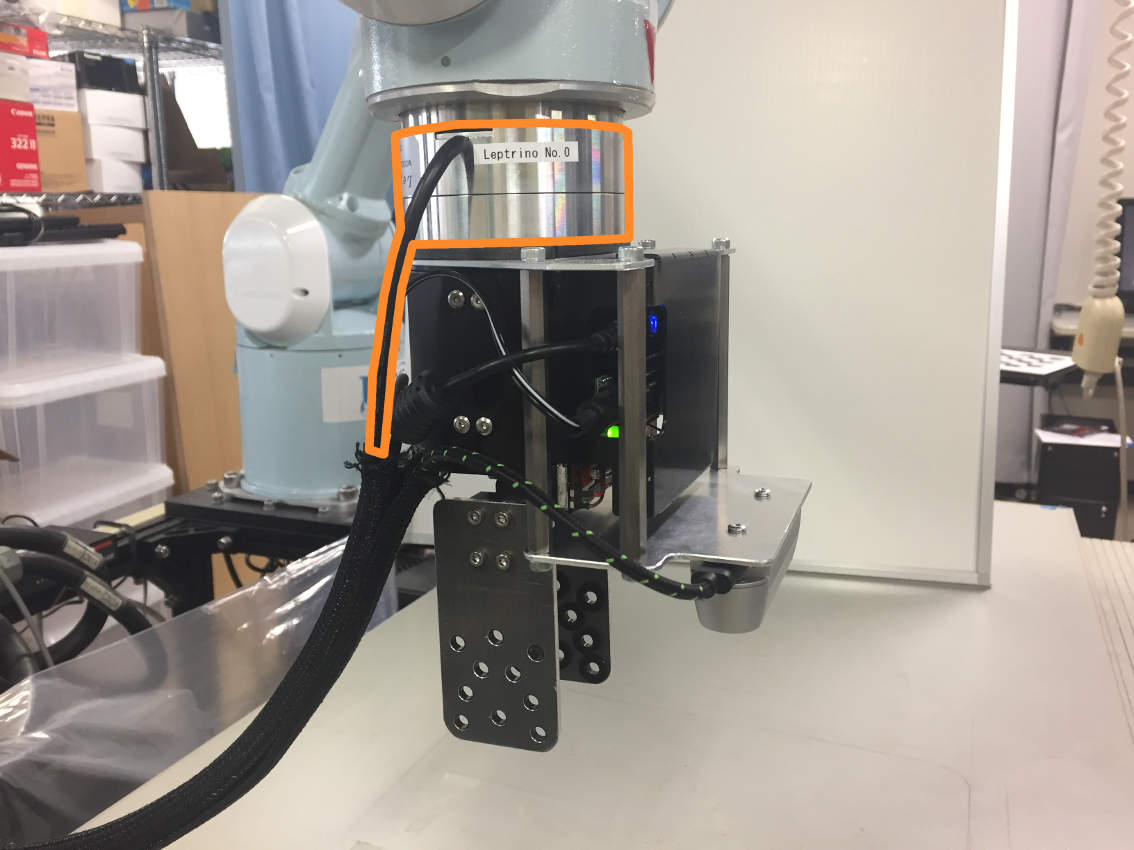
\includegraphics[width=.7\linewidth]{fig/chp3/ForceSensor.jpg}
    \caption{Six-axis Leptrino force sensor mounted on the wrist.}
    \label{fig:system:force-sensor-install}
\end{figure}

本センサの性能パラメータを表\ref{tab:system:force-sensor-spec}に示す．
データシートに基づき，本センサの力の分解能は以下の通り計算される：

\begin{equation}
\begin{split}
\text{分解能} &= \text{定格荷重} \times \text{分解能} \\
&= 500\;\mathrm{N} \times (1 / 4000) \\
&= 0.125\;\mathrm{N}
\end{split}
\end{equation}

% \begin{figure}[ht]
%     \centering
%     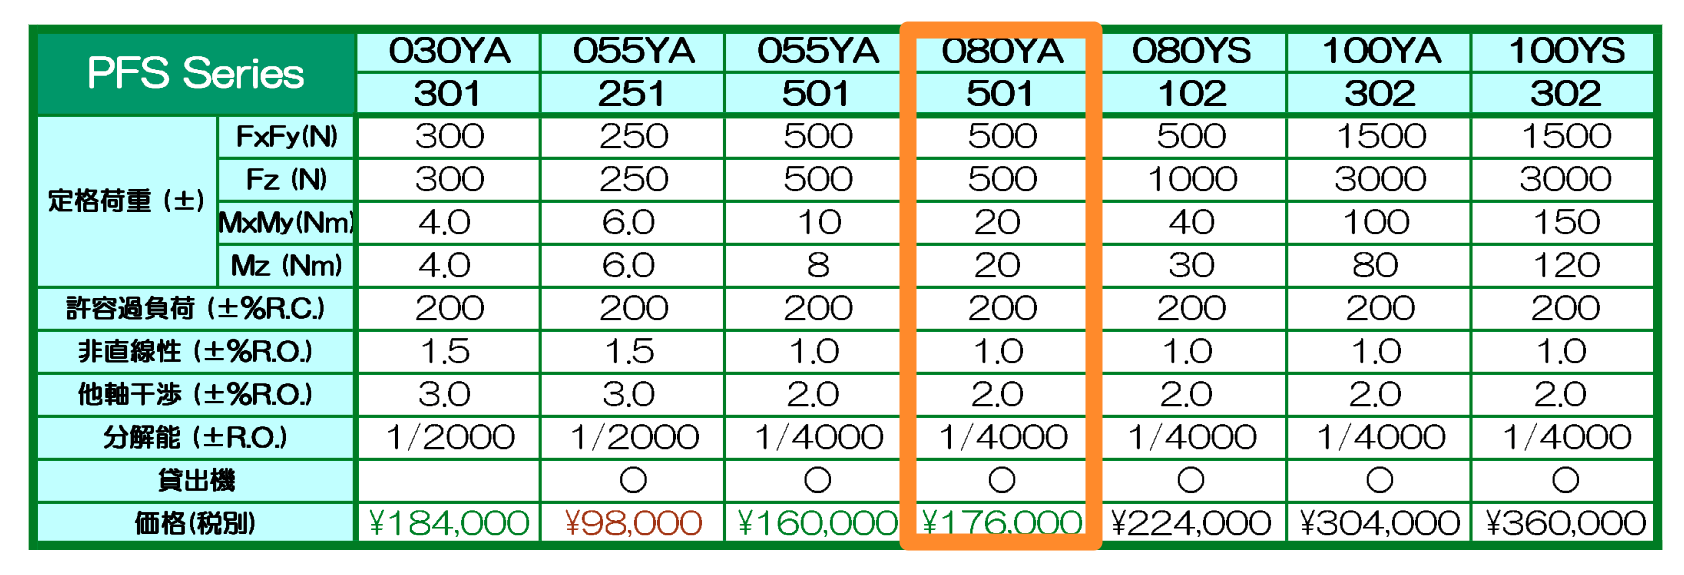
\includegraphics[width=1\linewidth]{fig/chp3/ForceSensor-performence.png}
%     \caption{Specification sheet of the PFS080YA501U6S.}
%     \label{fig:system:force-sensor-spec}
% \end{figure}
\begin{table}[ht]
  \centering
  \caption{Main specifications of the PFS080YA501U6S \cite{leptrino_6axis_force_sensor}.}
  \label{tab:system:force-sensor-spec}
  \begingroup
  \footnotesize
  \setlength{\tabcolsep}{4pt}
  \renewcommand{\arraystretch}{0.8}
  \begin{tabular}{@{}ll@{}}
    \toprule
    Item & Specification \\
    \midrule
    % Model & PFS080YA501U6 \\
    Rated force capacity ($F_x$, $F_y$, $F_z$) & $\pm 500$ N \\
    Rated moment capacity ($M_x$, $M_y$, $M_z$) & $\pm 20$ N$\cdot$m \\
    % Allowable overload & $\pm 200\%$ R.C. \\
    % Nonlinearity & $\pm 1.0\%$ R.O. \\
    % Inter-axis interference & $\pm 2.0\%$ R.O. \\
    Resolution & $1/4000$ \\
    \bottomrule
  \end{tabular}
  \endgroup
\end{table}

% 力覚情報は，特にツールと対象表面との接触が重要となる皮むき動作において有効であり，接触状態の確認および制御入力の設計に用いた．
% また，本論文では，3Dモデルに基づく幾何学的解析に加えて，接触に伴う力学的な情報も操作設計の一部として扱うため，力覚センサはそのための共通計測基盤として位置づけられる．
力覚情報は，皮むき動作では接触状態の監視と力フィードバック制御の入力として，把持研究では把持安定性の評価の補助情報として用いた．
このように，力覚センサは3Dモデルを補完する計測手段として，接触を伴うタスクにおいて重要な役割を担う．

\subsection{視覚センサ}
\label{sec:system:hardware:vision-sensor}

対象物および作業環境の3D情報取得には，Intel RealSense D435 を用いた．
\begin{revisionblock}
本センサはRGB画像と深度画像を同時に取得できるRGB-Dカメラである．
本研究では，軌道，把持候補，容積を計算するための三次元幾何に加え，皮むき済み領域の識別などに色情報も必要となるため，両者を同一装置，同一視点で取得できるRGB-D方式を採用した．
レーザスキャナ等は条件によってより高精度な距離計測が可能であるが，色情報を得る別カメラとセンサ間校正が必要になり，家庭用システムで重視される小型性，構成の簡潔さ，およびコストの面で不利となる．
一方，RGB-D方式にも，鏡面反射，透明・半透明物体，液面，遮蔽および距離条件による欠測・ノイズがある．
そこで，本研究では反射面を含めて常に安定に計測できるとは仮定せず，多視点計測，外れ値除去，および後述する精度評価を組み合わせ，対象範囲で利用可能な点群を得る．
\end{revisionblock}
図\ref{fig:system:robot-camera}のように，カメラは主としてグリッパ前面に取り付け，ロボットアームの動作により視点を変化させることで，複数視点から点群を取得した．
同時に異なる角度から点群を撮影する目的で，RealSense D435を両アームに取り付けた．

\begin{figure}[ht]
    \centering
    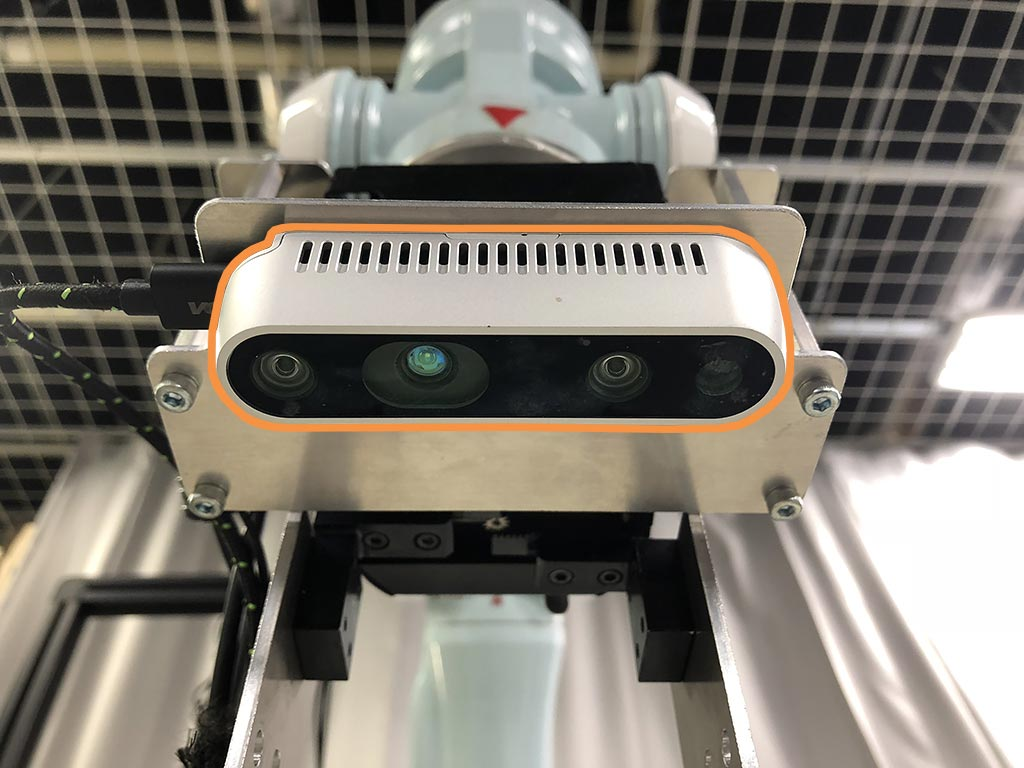
\includegraphics[width=.7\linewidth]{fig/chp3/Realsense.jpg}
    \caption{Intel RealSense D435 mounted on the wrist.}
    \label{fig:system:robot-camera}
\end{figure}

取得した点群は，各時刻におけるロボット姿勢とカメラの取り付け関係に基づいて世界座標系へ変換し，合成した3Dモデルとして利用する．
この3Dモデルは，注ぐ動作では容器内部形状の推定と容積計算に，皮むき動作では食材表面形状の取得とツール軌道生成に，安定把持では接触候補点の生成と把持安定性評価に用いられる．



\subsection{座標系定義とカメラキャリブレーション}
\label{sec:system:camera_calibration}

%%%%%
% \subsection{座標系定義とカメラキャリブレーション}
\label{sec:system:pointcloud:acquisition:calibration}

\paragraph{座標系の定義と接続関係}
\label{sec:system:hardware:coordinate-system}

本システムでは，RGB-Dカメラで取得した点群，ロボット手先の位置姿勢，
および各タスクにおけるツール先端位置を同一の基準で扱うため，複数の座標系を定義する．
各ロボットベース座標系の軸方向は，ロボット前方を$x$軸，
ロボットから見て左方向を$y$軸，鉛直上方を$z$軸とした．
回転の表現には$x$-$y$-$z$軸周りのオイラー角を用い，
各回転角度を$\alpha,\beta,\gamma$と表す．
正の回転方向は，各回転軸に対する右手系の正方向に従うものとする．

本論文では，以下の座標系を用いる．

\begin{enumerate}
  \item \textbf{ロボットベース座標系} $\Sigma_{B}$（Base）：
  各ロボットの基座中央を原点とする座標系である．
  双腕構成では，左腕のベース座標系を$\Sigma_{B_L}$，
  右腕のベース座標系を$\Sigma_{B_R}$と表す．
  各ロボットの関節角から得られる順運動学は，まず各ベース座標系を基準として計算される．

  \item \textbf{世界座標系} $\Sigma_{W}$（World）：
  本論文で扱う全タスクの共通基準座標系であり，
  左腕ロボットのベース座標系$\Sigma_{B_L}$と一致させる．
  すなわち，$\Sigma_W \equiv \Sigma_{B_L}$である．
  取得した点群，操作対象物，ツール先端位置，および左右腕の動作目標は，
  最終的にこの世界座標系上で記述する．

  \item \textbf{ロボット手先座標系} $\Sigma_{H}$（Hand）：
  ロボットアームの手首先端または手先フランジに固定された座標系であり，
  ロボットの移動指令およびツール座標系設定の基準となる．
  左腕と右腕を区別する場合は，それぞれ$\Sigma_{H_L}$，$\Sigma_{H_R}$と表す．

  \item \textbf{カメラ座標系} $\Sigma_{C}$（Camera）：
  RGB-Dカメラの光学中心を原点とし，
  カメラの光学軸を$z$軸とする座標系である．
  深度画像から復元された点群は，まずこの座標系で表される．

  \item \textbf{ツール座標系} $\Sigma_{T}$（Tool）：
  各タスクで使用するツールやエンドエフェクタの操作を容易にするため，
  ユーザが必要に応じて定義する座標系である．
  原点は，ピーラーの刃先，容器把持点，指先中心，包丁刃先など，
  作業において制御したい点に設定する．
  姿勢はツールの機能方向に合わせて定義し，
  手先座標系$\Sigma_H$に対する固定変換として与える．
\end{enumerate}

これらの座標系は，世界座標系$\Sigma_W$を基準として接続される．
左腕については，$\Sigma_W$と$\Sigma_{B_L}$が一致するため，
左腕手先の世界座標系における姿勢は順運動学から直接得られる．
一方，右腕については，右腕ベース座標系$\Sigma_{B_R}$から
左腕ベース座標系$\Sigma_{B_L}$への変換を介して，
右腕手先の姿勢を世界座標系へ変換する．

双腕ロボットの二つのベース座標系間の変換は，
同一位置に固定したChArUcoボードを左右のカメラから観測することで同定した．
これにより，左右のロボットで計算された手先位置，
左右のカメラで取得された点群，および各タスクの操作点を，
同一の世界座標系$\Sigma_W$上で扱うことができる．
% PA10-7Cを用いた構成では，両腕のベース座標系間の距離は$Y$軸方向に804\,mmであり，
% DENSO VS-050を用いた構成のベース配置については
% \ref{sec:system:configuration-changes:hardware}節で述べる．

手先座標系は，各ロボットの関節角と順運動学により，
親となるベース座標系に対する姿勢が得られる．
カメラ座標系は，カメラキャリブレーションにより，
手先座標系，ツール座標系，または1軸サーボカメラアームの関節座標系に対する
取り付け関係として決定される．
また，ツール座標系は，各タスクのツールやエンドエフェクタに応じてユーザが定義し，
手先座標系に対する固定変換として扱う．

手先に固定されたカメラで取得した点$\bm{p}$を同次座標で表すと，
カメラ座標系$\Sigma_C$から世界座標系$\Sigma_W$への変換は次式で記述される．

\begin{equation}
  {}^{W}\bm{p}
  =
  {}^{W}\bm{T}_{H}
  \cdot
  {}^{H}\bm{T}_{C}
  \cdot
  {}^{C}\bm{p}
  \label{eq:system:transform_chain}
\end{equation}

ここで，${}^{W}\bm{T}_{H}$は手先座標系から世界座標系への同次変換行列である．
左腕では順運動学により直接得られ，右腕ではベース間変換を含めて計算される．
${}^{H}\bm{T}_{C}$は手先座標系に対するカメラ座標系の取り付け位置姿勢，
${}^{C}\bm{p}$はカメラ座標系における点の位置ベクトルである．
なお，カメラがツールまたは1軸サーボカメラアームを介して取り付けられる場合には，
式\eqref{eq:system:transform_chain}中の${}^{H}\bm{T}_{C}$を，
該当する取り付け変換に置き換えて用いる．

同様に，ツール先端の姿勢は次式で表される．

\begin{equation}
  {}^{W}\bm{T}_{T}
  =
  {}^{W}\bm{T}_{H}
  \cdot
  {}^{H}\bm{T}_{T}
  \label{eq:system:tool_transform}
\end{equation}

ここで，${}^{H}\bm{T}_{T}$は各タスクで定義される
手先座標系からツール座標系への固定変換である．
ツール座標系を用いることで，ロボットの手先フランジではなく，
実際に作業を行うツール先端を目標位置・姿勢へ直接誘導できる．
例えば，ピーラーでは刃先位置，注ぎ作業では容器把持部または容器姿勢，
安定把持では指先接触点や包丁の刃先位置を基準として動作を記述できる．
PA10-7Cでは三菱重工が提供するPAライブラリを用いて手先の位置姿勢を制御するため，
ロボット手先に対するツール座標系$\Sigma_T$の位置・姿勢を
プログラム上で調整可能とした．
PA10-7Cにおけるツール座標系の設定例を図\ref{fig:system:tool-coordinate}に示す．

\begin{figure}[ht]
    \centering
    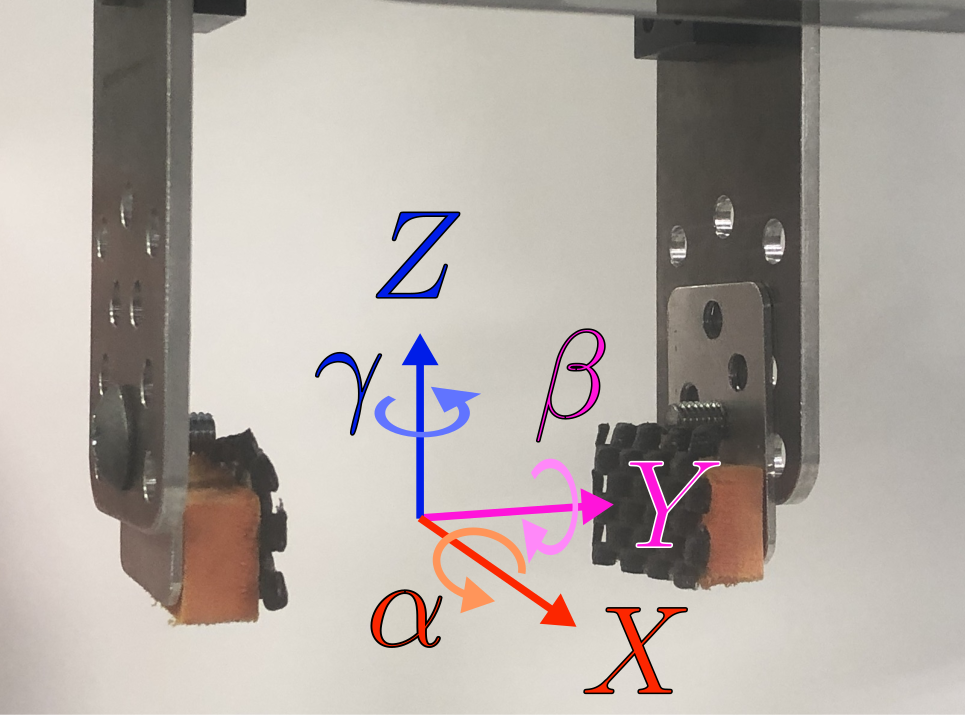
\includegraphics[width=0.7\linewidth]{fig/chp3/ToolCoordinate.png}
    \caption{Tool coordinate system.}
    \label{fig:system:tool-coordinate}
\end{figure}

\paragraph{カメラキャリブレーションと外部パラメータ}


RGB-Dカメラから取得した点群を多視点で合成するためには，
深度画像から復元された各点を，各撮影時のカメラ姿勢に基づいて
世界座標系へ変換する必要がある．
本研究では，カメラ内部パラメータ，手先座標系に対するカメラの取り付け位置姿勢，
左右アームのベース座標系間の変換，およびDENSO VS-050で用いた
1軸サーボカメラアームの角度依存変換を事前に同定した．

カメラ内部パラメータは，キャリブレーションボードを用いた通常の
カメラキャリブレーションにより取得し，深度画像からカメラ座標系の点群へ
逆投影する際に用いた．
以下では，多視点点群合成に直接関係する外部パラメータについて述べる．

\paragraph{ハンドアイキャリブレーション}
\label{sec:system:hand_eye}

手先に固定したカメラを用いる構成では，ロボット手先座標系 $\Sigma_H$ に対する
カメラ座標系 $\Sigma_C$ の固定変換 ${}^{H}\bm{T}_{C}$ を
ハンドアイキャリブレーションにより求めた．
具体的には，ChArUcoボードを作業空間内に静置し，ロボット手先を複数姿勢に
移動させながらボードを撮影した．
各画像から得られるボードとカメラの相対姿勢，およびロボットの順運動学から得られる
手先姿勢を用いて，OpenCVの
\texttt{calibrateRobotWorldHandEye} により
${}^{H}\bm{T}_{C}$ を推定した．
得られた変換は環境設定ファイルに保存し，実行時にはロボットの手先姿勢と合成して，
カメラ座標系で得られた点群を世界座標系へ変換する．

また，双腕ロボットでは左右アームのベース座標系を統一する必要がある．
本論文では左アームのベース座標系を世界座標系 $\Sigma_W$ として定義し，
同一のChArUcoボードを左右アームから観測することで，右アームのベース座標系
$\Sigma_{B_R}$ から左アームのベース座標系 $\Sigma_{B_L}$ への変換を求めた．
左右の観測から得られるボード姿勢をそれぞれ
${}^{B_L}\bm{T}_{\mathrm{cb}}$，
${}^{B_R}\bm{T}_{\mathrm{cb}}$ とすると，ベース座標系間の変換は次式で表される．

\begin{equation}
  {}^{B_L}\bm{T}_{B_R}
  =
  {}^{B_L}\bm{T}_{\mathrm{cb}}
  \left({}^{B_R}\bm{T}_{\mathrm{cb}}\right)^{-1}
  \label{eq:system:base_to_base}
\end{equation}

これにより，左右のカメラで取得した点群，および各アームで計算された操作点を，
同一の世界座標系上で扱うことが可能となる．

\paragraph{1軸サーボカメラアームのキャリブレーション}
\label{sec:system:servo_cam_calib}

\begin{figure}[ht]
  \centering
  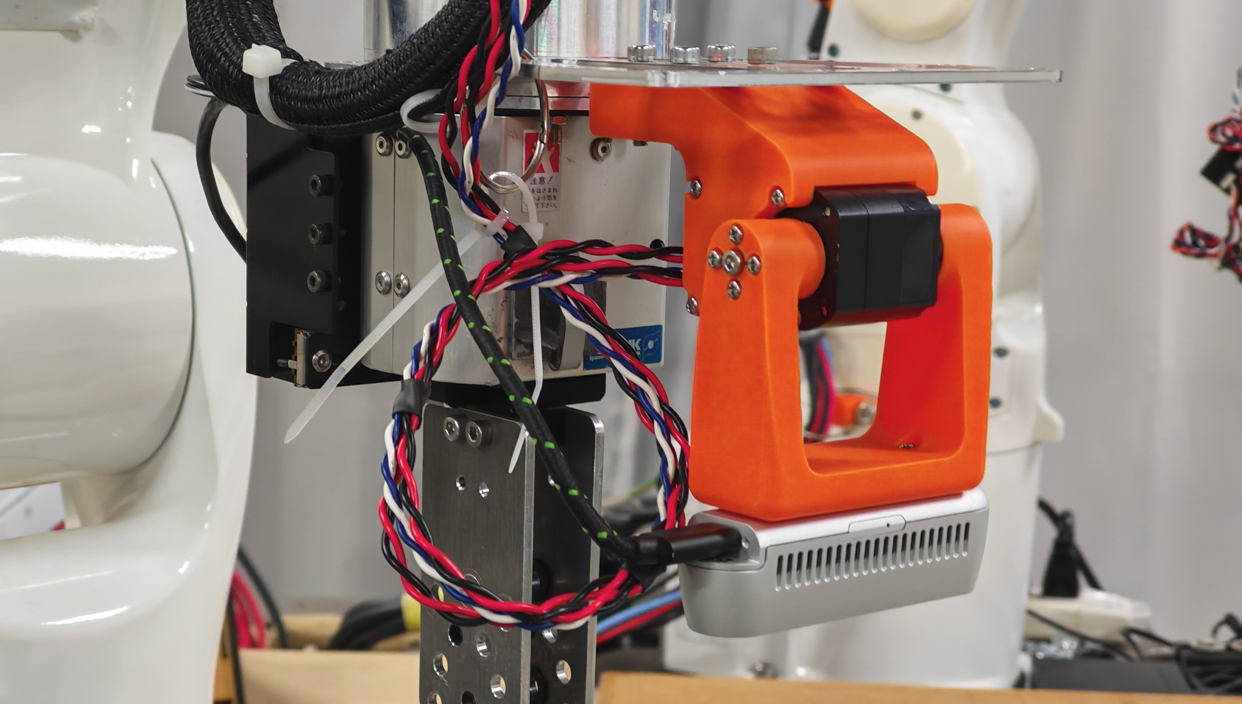
\includegraphics[width=.7\linewidth]{fig/chp3/chp3_new_robot_camera_arm.png}
  \caption{The camera arm for DENSO VS-050.}
  \label{fig:system:robot-camera-arm-denso}
\end{figure}

DENSO VS-050を用いたロボットシステムでは，ロボットの可動範囲の制約を補うため，
RGB-Dカメラを1軸サーボアームに取り付けた
（図\ref{fig:system:robot-camera-arm-denso}）．
このカメラアームはロボット手先に固定されているため，カメラ姿勢は手先座標系
$\Sigma_H$ を上位座標系として，サーボ角 $\theta$ に応じて変化する．
したがって，固定カメラ構成で用いた一定値の ${}^{H}\bm{T}_{C}$ ではなく，
角度依存の変換 ${}^{H}\bm{T}_{C}(\theta)$ を用いる．

本研究では，サーボカメラアームを1自由度の回転関節としてモデル化した．
手先座標系 $\Sigma_H$ からカメラ座標系 $\Sigma_C$ への変換は，
サーボ関節座標系 $\Sigma_J$ を介して次式で表される．

\begin{equation}
  {}^{H}\bm{T}_{C}(\theta)
  =
  {}^{H}\bm{T}_{J}
  \begin{bmatrix}
    R(\bm{a},\,\theta) & \bm{0} \\
    \bm{0}^{\top} & 1
  \end{bmatrix}
  {}^{J}\bm{T}_{C}
  \label{eq:system:servo_camera_model}
\end{equation}

ここで，$\bm{a}$ はサーボ関節座標系における回転軸，
$\theta$ はサーボ関節角である．
また，${}^{H}\bm{T}_{J}$ は手先座標系からサーボ関節座標系への固定変換，
${}^{J}\bm{T}_{C}$ はサーボ関節座標系からカメラ座標系への固定変換である．

これらのパラメータは，複数のサーボ角 $\theta$ においてChArUcoボードを観測し，
各角度で得られたカメラ姿勢と式\eqref{eq:system:servo_camera_model}の予測値が
最も一致するように，非線形最小二乗法により推定した．

実行時には，現在のサーボ角 $\theta$ から ${}^{H}\bm{T}_{C}(\theta)$ を計算し，
ロボットの順運動学により得られる手先姿勢と合成することで，
世界座標系におけるカメラ姿勢を求める．

\begin{equation}
  {}^{W}\bm{T}_{C}(\theta)
  =
  {}^{W}\bm{T}_{H}
  {}^{H}\bm{T}_{C}(\theta)
  \label{eq:system:world_camera_servo}
\end{equation}

以上のキャリブレーションにより，固定カメラ構成および1軸サーボカメラアーム構成の
いずれにおいても，RGB-Dカメラで取得した点群を世界座標系へ変換し，
多視点点群として合成できる．




\subsection{エンドエフェクタ設計}
\label{sec:system:hardware:end-effector}

\subsubsection{平行グリッパ}
\label{sec:system:hardware:parallel-gripper}
力覚センサの先端には，三菱電機製の平行グリッパ1E-HM01 HANDを取り付けた（図\ref{fig:system:parallel-gripper}）．
本グリッパの指先に取り付けられたアルミ板には，様々な姿勢でツールを装着できるように多数の穴が設けられており，各研究の要件に応じてエンドエフェクタを交換可能な構造となっている．

\begin{figure}[ht]
    \centering
    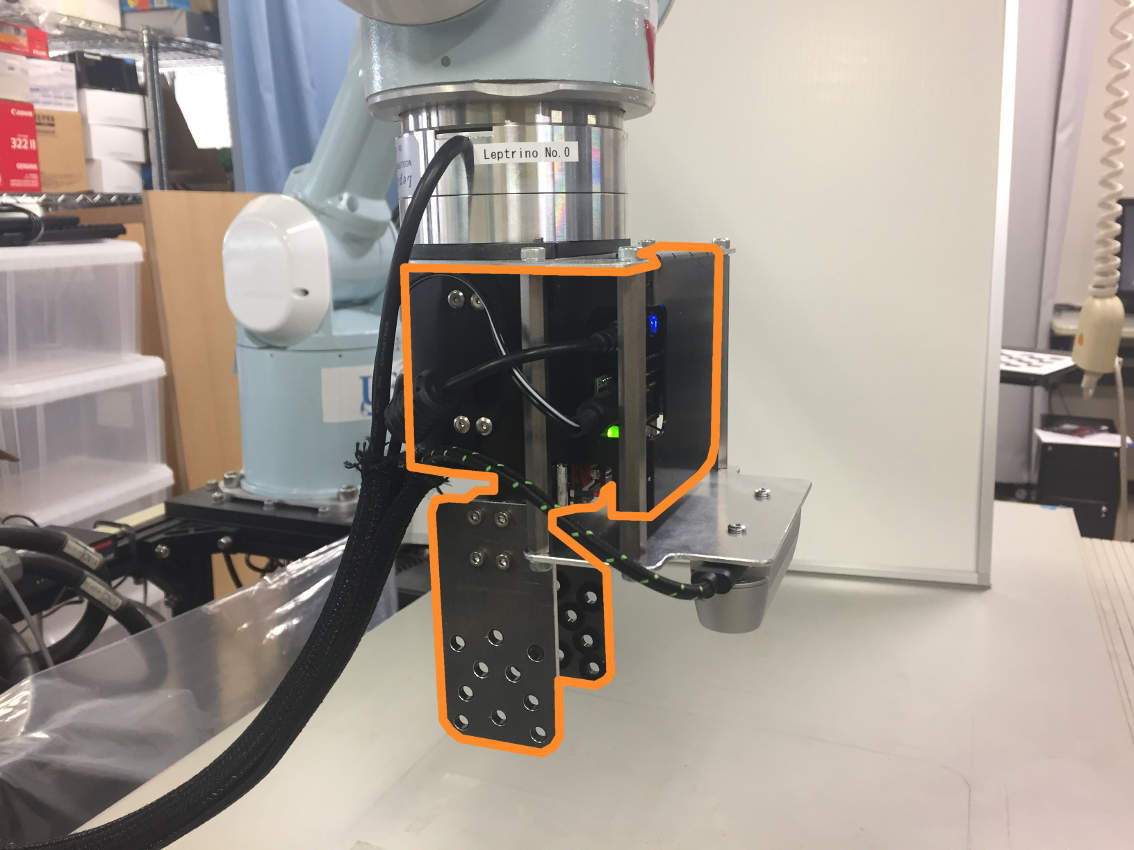
\includegraphics[width=.7\linewidth]{fig/chp3/Gripper.jpg}
    \caption{Parallel gripper indicated by the orange frame.}
    \label{fig:system:parallel-gripper}
\end{figure}

本論文では，この平行グリッパを，タスクに応じたエンドエフェクタを取り付けるための共通インタフェースとして用いた．
注ぎ用エンドエフェクタでは，指先アルミ板に容器把持用の接触部を取り付け，容器の縁部または外周部を把持した．
皮むき用エンドエフェクタでは，ピーラー固定部および食材固定用の$V$字溝部を同じ取付穴列に固定し，道具先端および食材固定位置を再現性よく設定した．
安定把持用エンドエフェクタでは，右腕側の平行グリッパを包丁固定用の高剛性把持部として利用し，左腕側は食材表面への接触点を柔軟に選択するため指型ハンドに置き換えた．


\subsubsection{皮むき用エンドエフェクタ}
\label{sec:system:hardware:peeling-end-effector}
皮むき動作では，片方の腕でピーラーを操作し，もう片方の腕で食材を固定する必要がある．
このため，両アームとも平行グリッパを基盤としつつ，役割に応じて異なるエンドエフェクタを装着した．

ツール側のエンドエフェクタ（図\ref{fig:system:peeling-end-effector-peeler}）としては，ピーラーをロボット手先へ固定するためのパーツを設計した．
このパーツにより，ピーラーの刃先位置と姿勢をツール座標系として明確に定義でき，食材表面形状に基づいて生成した軌道に従って刃先を安定に移動させることが可能となる．

\begin{figure}[ht]
    \centering
    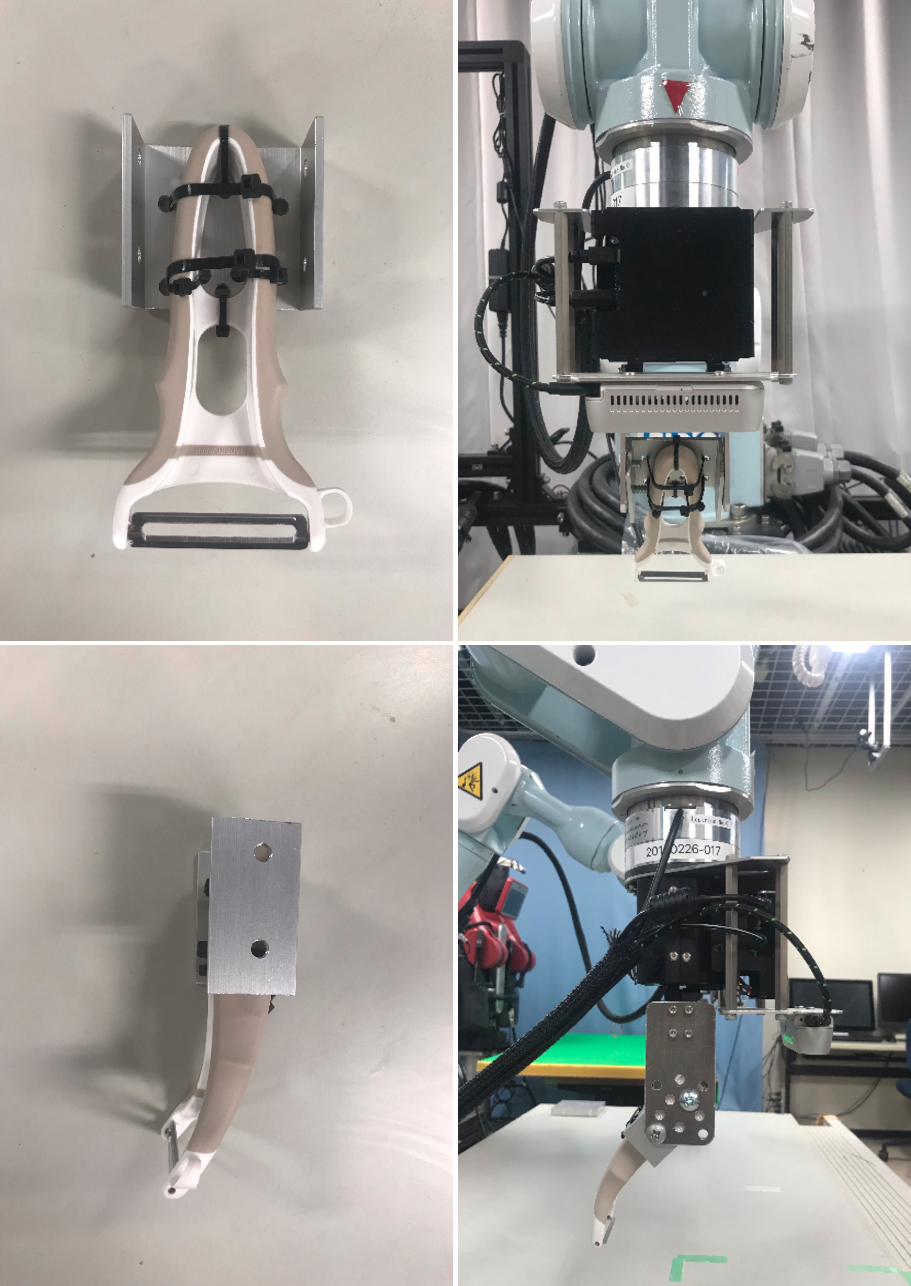
\includegraphics[width=.7\linewidth]{fig/chp3/PeelingEndeffector-2.pdf}
    \caption{Peeler-side end effector for the peeling task.}
    \label{fig:system:peeling-end-effector-peeler}
\end{figure}

食材固定側のエンドエフェクタとしては，食材に刺した串を安定に固定するための専用ぱパーツを用いた．
細長い串は通常の平行グリッパでは毎回同じ位置に保持することが難しいため，$V$字溝を有する把持部を設け，串が一定位置に自然に収まるように設計した（図\ref{fig:system:peeling-end-effector-food}）．
これにより，食材の姿勢再現性が向上し，皮むき軌道の安定な実行が可能となる．

\begin{figure}[ht]
    \centering
    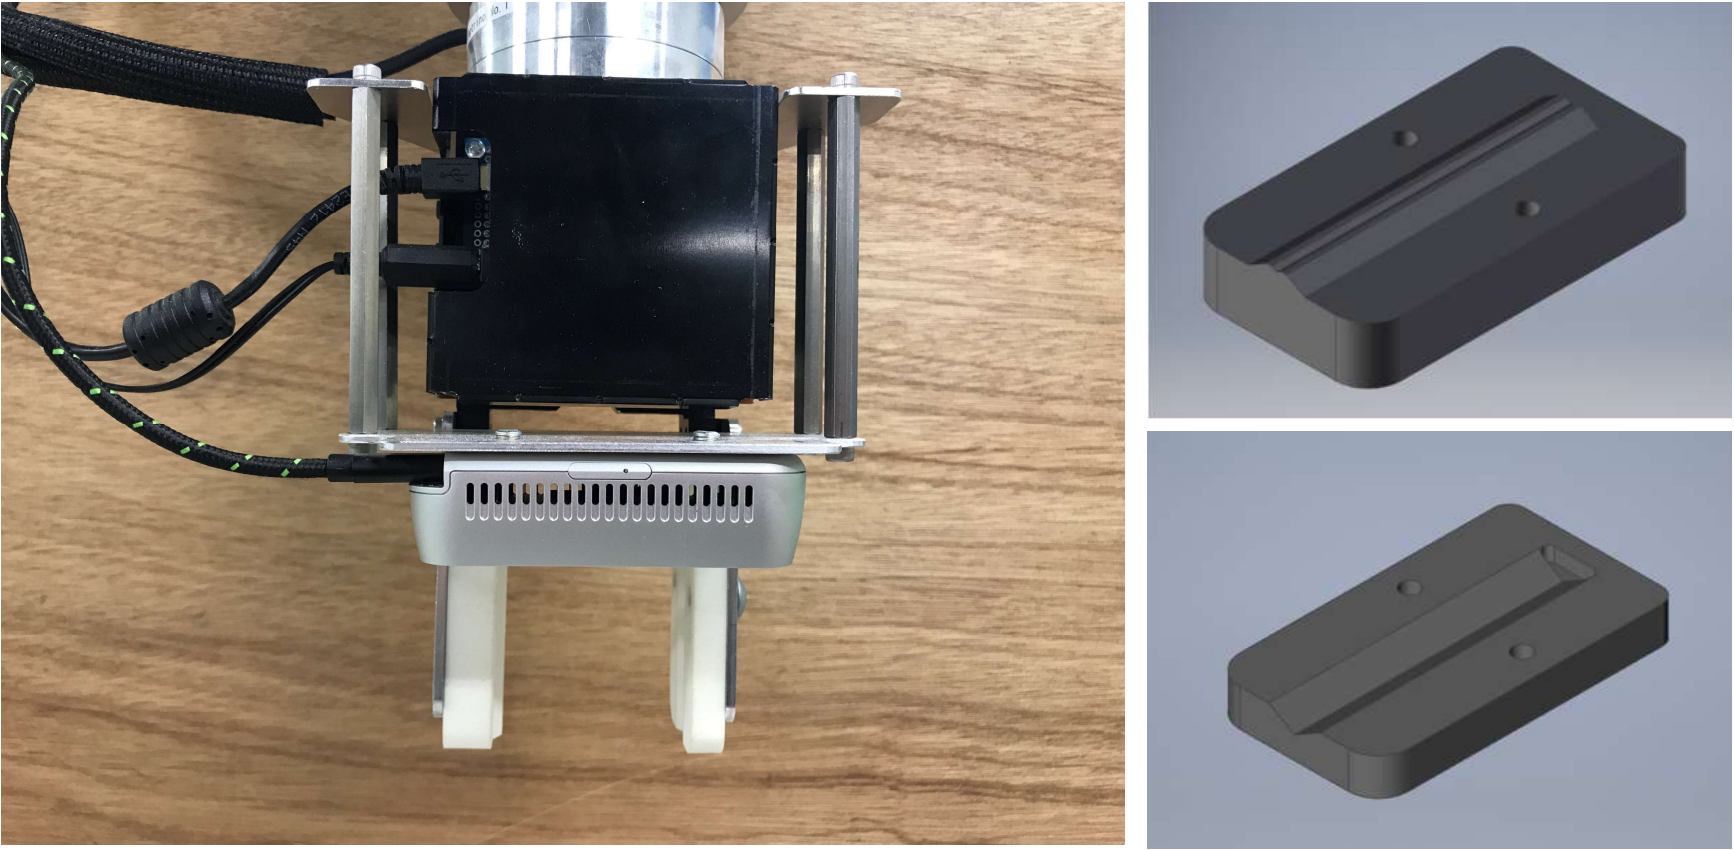
\includegraphics[width=.5\linewidth]{fig/chp3/PeelingEndeffector-1.png}
    \caption{Food-fixation end effector for the peeling task.}
    \label{fig:system:peeling-end-effector-food}
\end{figure}

\subsubsection{注ぎ用エンドエフェクタ}
\label{sec:system:hardware:pouring-end-effector}
注ぐ動作では，各種容器を安定に把持し，必要に応じて持ち上げ，傾ける必要がある．
そこで，平行グリッパを基盤とし，その指先アルミ板に容器把持用のエンドエフェクタを取り付けた．
本研究では，対象容器の形状差に対応するため，2種類のエンドエフェクタを用いた．

第1のエンドエフェクタ（図\ref{fig:system:pouring-end-effector-1}）は，ボウルやカップのように開口縁を有する容器を対象としたものである．
平行グリッパの開口幅（最大10\,cm）のみでは把持が困難な場合を想定し，容器本体ではなく縁部を把持できるように設計した．
また，把持時の摩擦力を高めるため，接触面には小型のスポンジを取り付けた．

\begin{figure}[ht]
    \centering
    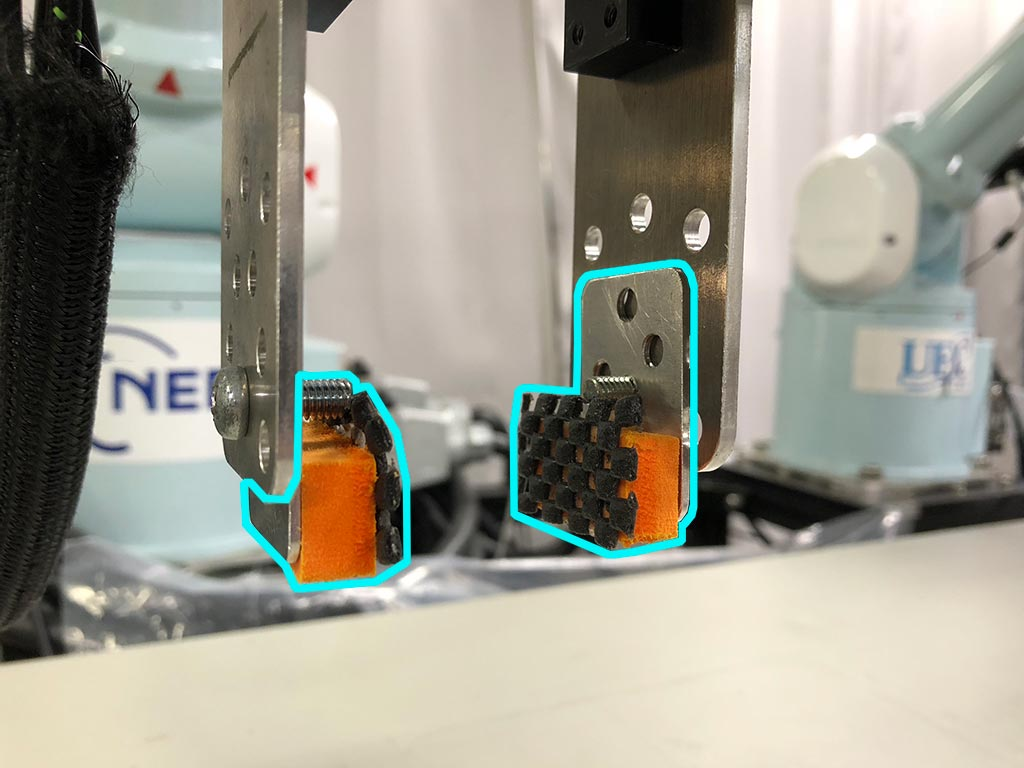
\includegraphics[width=.7\linewidth]{fig/chp3/PourEndFactor-1.jpg}
    \caption{End effector 1 for the pouring task.}
    \label{fig:system:pouring-end-effector-1}
\end{figure}

第2のエンドエフェクタ（図\ref{fig:system:pouring-end-effector-2}）は，外形寸法が比較的小さく，グリッパ開口幅内に収まる容器を確実に把持することを目的としたものである．
こちらも把持安定性向上のため，接触面に薄いスポンジを取り付けた．
このように，注ぐ動作におけるエンドエフェクタ設計では，容器形状の多様性に対して，把持を切り替えられることを重視した．

\begin{figure}[ht]
    \centering
    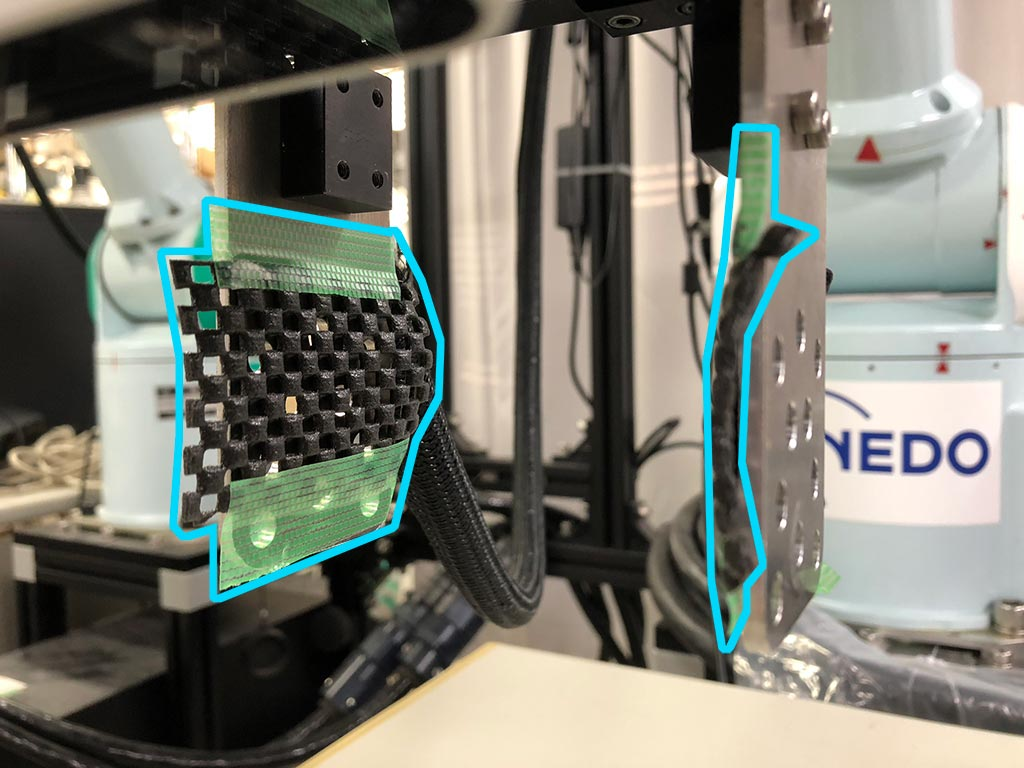
\includegraphics[width=.7\linewidth]{fig/chp3/PourEndFactor-2.jpg}
    \caption{End effector 2 for the pouring task.}
    \label{fig:system:pouring-end-effector-2}
\end{figure}

\subsubsection{安定把持用エンドエフェクタ}
\label{sec:system:hardware:holding-end-effector}
安定把持の研究では，左腕に食材把持用の指型ハンドを，右腕に包丁固定用の高把持力平行グリッパを装着した．
右アーム側の平行グリッパは，包丁をロボットへ剛結合することを目的としており，切断するときに発生する外力を安定に伝達できるようにした．
左アーム側では，食材形状に応じて接触点を柔軟に選択できることが重要であるため，多関節の指型ハンドを用いた．

食材把持用ハンドとしては，3軸2指のサーボハンドを用いた（図\ref{fig:system:finger-hand}）．
各指には FUTABAのサーボ RS405CB を使用し，最大トルクは48.0\,$\mathrm{kgf \cdot cm}$，角度分解能は0.1\,degである．
各指の関節構成は $z$-$y$-$y$-tip とし，指先位置を制御するために，ヤコビアンに基づく指関節のみの逆運動学を用いた．
この構成により，食材表面上に生成した候補接触点へ指先を誘導し，把持安定性の評価に基づいて適切な接触配置を実現できる．
\revise{指先は把持安定性の計算で仮定する点接触に近づけるため，食材に対する接触面を小さくした．また，包丁軌道と干渉せずに食材上面・側面の候補点へ届く指長と関節配置を採用し，カメラ観測時には指同士および指と食材による遮蔽が固定化しないよう，対象の提示姿勢を変更できる構成とした．}

\begin{figure}[ht]
    \centering
    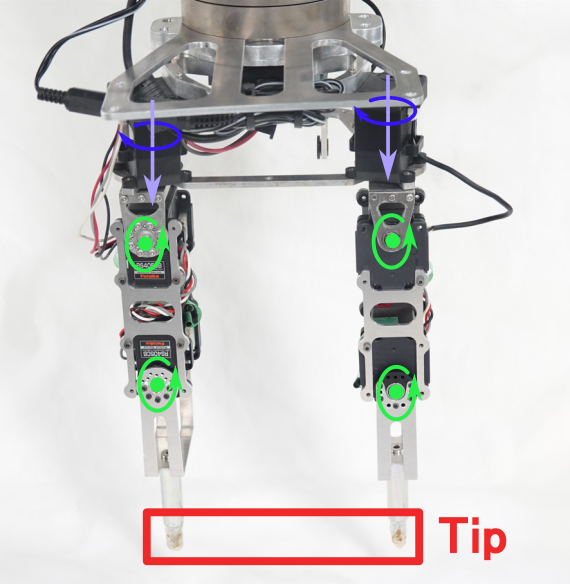
\includegraphics[width=.5\linewidth]{fig/chp3/ICRA_RobotHand.png}
    \caption{Finger hand used for holding.}
    \label{fig:system:finger-hand}
\end{figure}

このように，切断する時に把持におけるエンドエフェクタ設計では，包丁側には高剛性な固定機構を，食材側には形状適応性を有する多指ハンドを使用することで，切断時の外力と把持安定性の両立を図った．

% \subsection{座標系定義}
% \label{sec:system:hardware:coordinate-system}

% 各軸の向きはロボット前方を$x$軸，ロボットから見て左方向を$y$軸，鉛直上方を$z$軸とした．

% 双腕共同作業を統一的に記述するため，世界座標系を定義した．
% 世界座標系の原点は左アームのベース座標系と一致させ，各軸の向きも左アームのベース座標系と同様に設定した．
% 回転の表現には$x$-$y$-$z$軸周りのオイラー角を用い，各回転角度を$\alpha,\beta,\gamma$と表す．プラス回転方向は各回転軸に対して逆時計回りとした．

% また，各アームがお互いの動作を妨害せずに共同作業を可能とするため，両アームのベース座標系間の距離を$Y$軸方向に804\,mmとした．
% % Relative base transforms:
% % robot.denso.middle.base -> robot.denso.right.base (XYZABC, ABC in deg, Euler order XYZ):
% %   [0.433713, 0.759744, 0.064421, 1.607230, -0.778746, -92.196446]
% % robot.denso.right.base -> robot.denso.middle.base (XYZABC, ABC in deg, Euler order XYZ):
% %   [0.777336, -0.404764, -0.037188, -0.716564, -1.635894, 92.197139]

% \begin{figure}[ht]
%     \centering
%     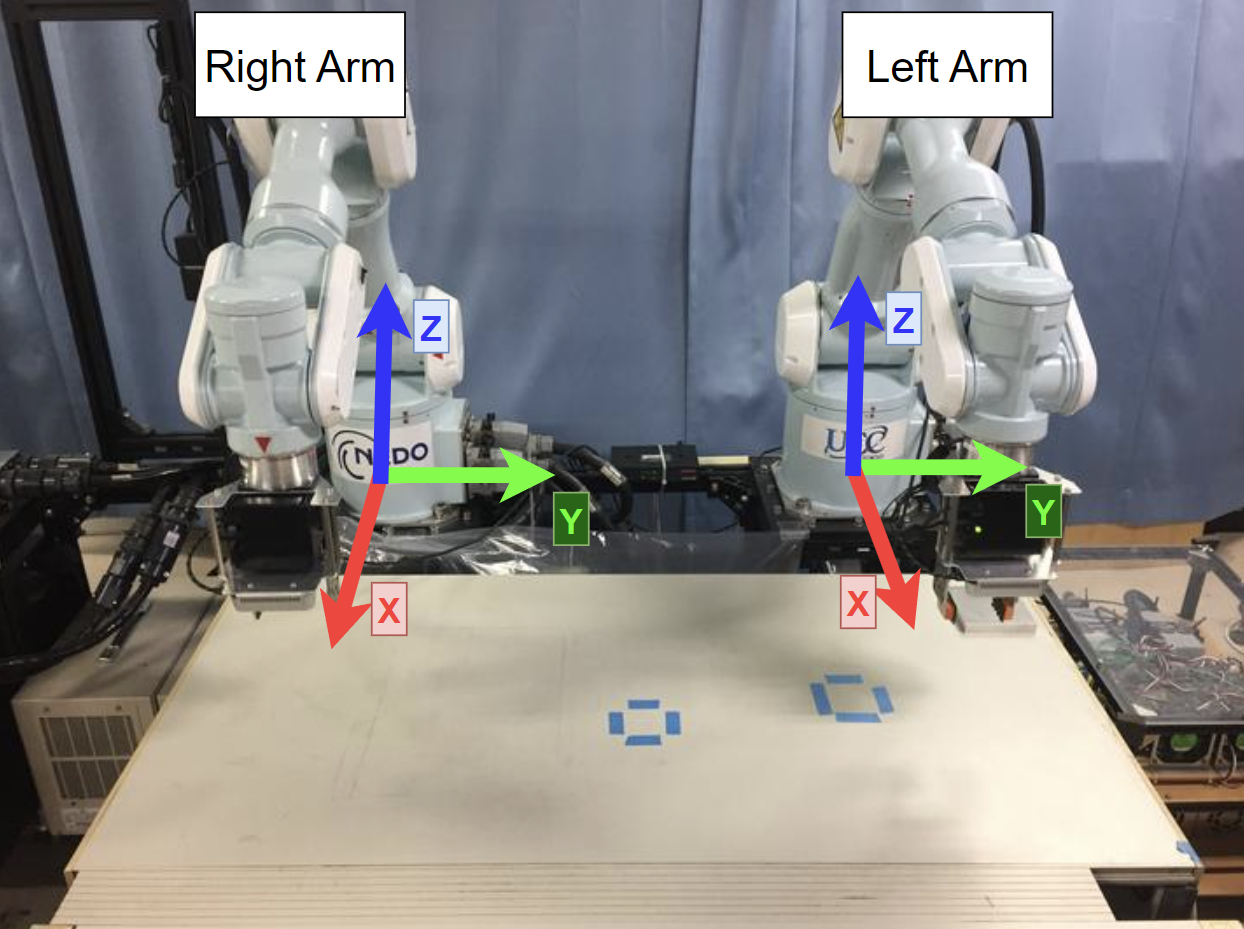
\includegraphics[width=0.8\linewidth]{fig/chp3/chp3_old_robot_coordinate.drawio.png}
%     \caption{The coordinate system of PA10-7C.}
%     \label{fig:system:robot-env-pa10}
% \end{figure}
% \begin{figure}[ht]
%     \centering
%     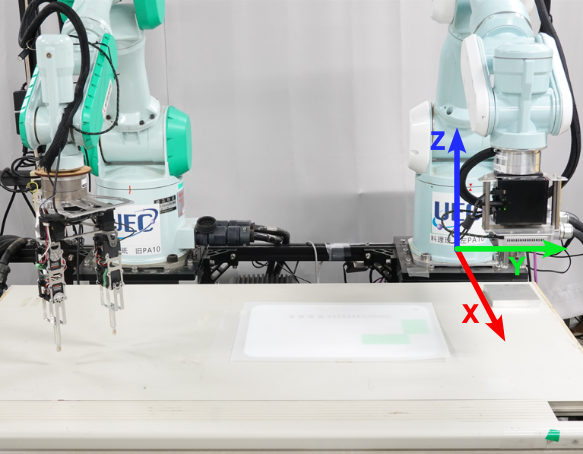
\includegraphics[width=.8\linewidth]{fig/chp3/ICRA_RobotEnv.png}
%     \caption{The coordinate system of PA10-7C. Right side robot is called [Left Arm]}
%     \label{fig:system:robot-env-pa10-alternative}
% \end{figure}
% \begin{figure}[ht]
%     \centering
%     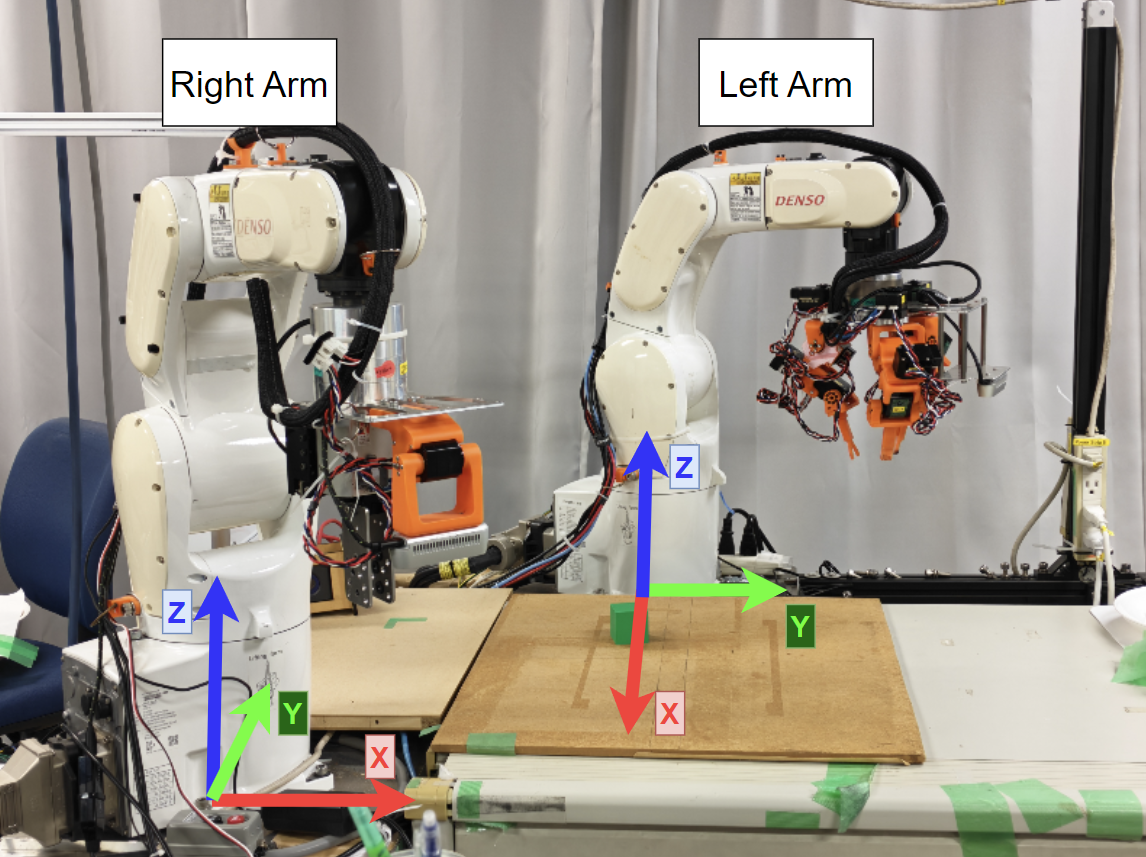
\includegraphics[width=.8\linewidth]{fig/chp3/chp3_new_robot_coordinate.drawio.png}
%     \caption{The coordinate system of DENSO VS-050.}
%     \label{fig:system:robot-env-denso-alternative}
% \end{figure}

% \paragraph{ツール座標系}

% ツール座標系は，ロボットが操作する道具の座標系である．
% 道具を目標の位置・姿勢へ誘導する際，ロボットの手先座標系を直接制御するよりも，道具先端に設定した座標系を制御するほうが直感的かつ高精度な動作記述が可能となる．

% PA10-7Cでは三菱重工が提供するPAライブラリを用いて手先の位置姿勢を制御する．
% 本研究では，ロボット手先にツールを装着した状態で各種作業を実行するため，以下のようにツール座標系を定義した．
% PA10手先座標系の原点は手先フランジの中心に位置し，姿勢はベース座標系に対して$Y$軸周りに180度回転させた姿勢である．
% ツール座標系の原点は装着したツールの中心（ピーラーであれば刃先，把持用エンドエフェクタであれば指先中心）に設定し，姿勢はPA10手先座標系から$Y$軸周りに180度回転させた姿勢，すなわちベース座標系と同一方向となるように定義した（図\ref{fig:system:tool-coordinate}）．
% 各種ツールに対応するため，ツール座標系の位置・姿勢はプログラム上で調整可能とした．

% \begin{figure}[ht]
%     \centering
%     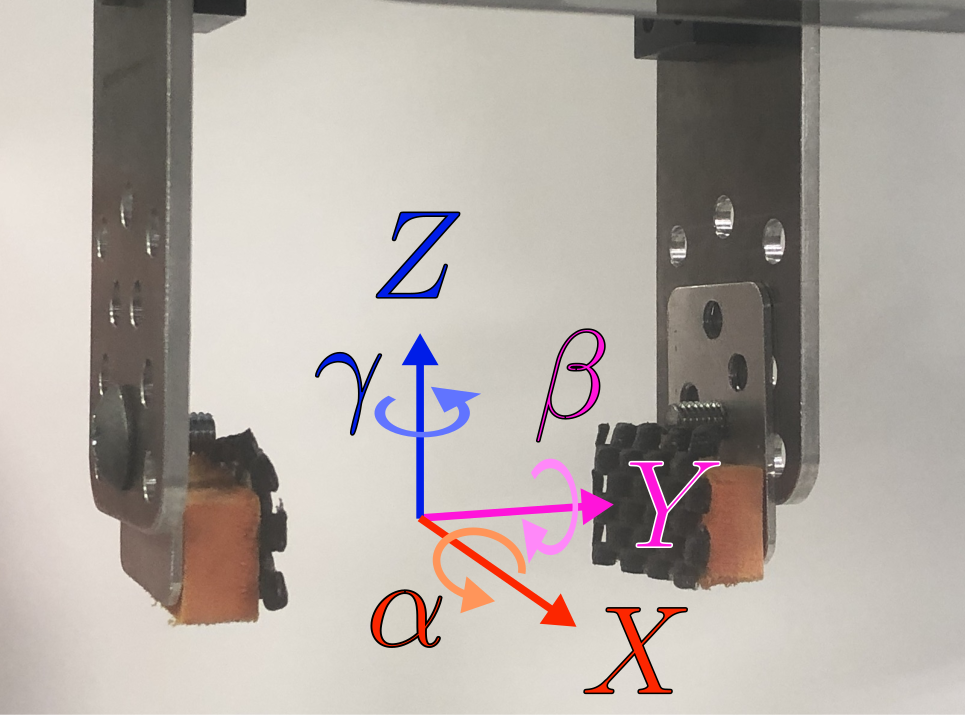
\includegraphics[width=0.7\linewidth]{fig/chp3/ToolCoordinate.png}
%     \caption{Tool coordinate system.}
%     \label{fig:system:tool-coordinate}
% \end{figure}

\section{システム構成：ソフトウェア}
\label{sec:system:software}

本研究を構成する三つの研究では，実施時期や要件の変化に伴い，ソフトウェア構成に段階的な変更が生じた．
しかし，点群処理アルゴリズムの本質（処理順番・パラメータ・出力仕様）は全研究で一貫している．
本節では，主に注ぐ・皮むきの研究で用いたOpenRTMベースのRTC統合アーキテクチャについて述べ，最後の把持の研究におけるソフトウェア構成の変更点を整理する．

\subsection{使用ライブラリ}
\label{sec:system:software:libraries}

\paragraph{librealsense}

librealsenseはIntel社がRealSenseシリーズのカメラを操作するために提供するクロスプラットフォームSDKである．
C++のほか，Python，MATLABなど複数のプログラミング言語に対応しており，PCLやOpenCV等のライブラリへのデータ受け渡しも容易である．
本ライブラリは，カメラに搭載された各種センサのデータ取得に加え，深度画像から点群データへの変換，カラー画像と深度画像の合成などのデータ処理機能を提供する．
本研究ではlibrealsense 2.11を用いた．

\paragraph{PCL（Point Cloud Library）}

\label{sec:system:software:pcl}

PCL（Point Cloud Library）は2次元・3次元の点群データを処理するためのオープンソースライブラリである\cite{PCL}．
フィルタリング，特徴量抽出，点群位置合わせ（Registration），近傍探索（KD-Tree），セグメンテーション，可視化など，点群処理に必要な機能がモジュール化されており，最新の研究手法を実装可能な拡張性を有する．
本研究ではPCL 1.8.0を用い，本章後半で述べる点群処理パイプラインの実装基盤とした．

\subsection{OpenRTMに基づくソフトウェアフレームワーク}
\label{sec:system:software:openrtm}
本研究では，RT-Middlewareの実装のひとつであるOpenRTM-aist\cite{RTM-aist}を用いてコンポーネント指向のロボット操作システムを構築した．
各ハードウェアをRT-Component（ハードウェアを操作するための独立プログラム，以下RTCとよぶ）として作成し，RTC-handle\cite{rtc_handle}を用いてこれらを接続することで，システム全体を統括した．
Pythonのメインスクリプトから関数をコールすることで，RTC-handleを介して各RTCに指令を送る構成とした．

\paragraph{システム全体の接続構成}

図\ref{fig:system:overall-connection-architecture}にシステム全体の接続構成を示す．
図のPA10 PCはロボット制御に特化した専用PCであり，その他の処理は共通PC上で実行される．

% TODO:这软件张图需要修复
\begin{figure}[ht]
    \centering
    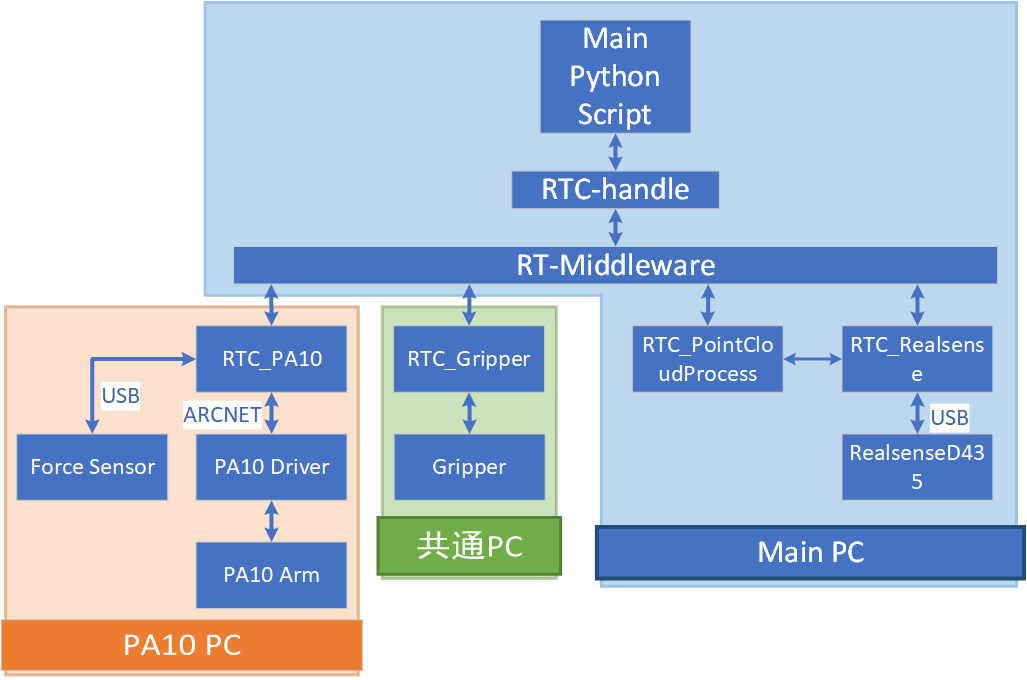
\includegraphics[width=0.9\linewidth]{fig/chp3/AllConnection.png}
    \caption{Overall connection architecture.}
    \label{fig:system:overall-connection-architecture}
\end{figure}

\paragraph{RTC\_PA10}

RTC\_PA10はPA10を操作するためのRTCである．
このRTCは専用PC（図\ref{fig:system:overall-connection-architecture}のPA10 PC）上で常時実行され，三菱重工が提供するPAライブラリを用いてARCNET経由でPA10のドライバと通信し，PA10ロボットを制御する．
リアルタイムの力のフィードバック制御を実現するため，力覚センサの操作メソッドも本RTCに組み込まれている．
RTC\_PA10のポート構成を図\ref{fig:system:rtc-pa10}に示す．

\begin{figure}[ht]
    \centering
    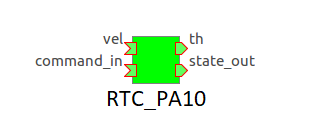
\includegraphics[width=0.4\linewidth]{fig/chp3/PA10Diag.png}
    \caption{Port configuration of RTC\_PA10.}
    \label{fig:system:rtc-pa10}
\end{figure}

\paragraph{RTC\_Gripper}

RTC\_Gripperは手先のグリッパを制御するためのRTCであり，グリッパの開閉動作を制御する．
保守性を考慮し，各腕のグリッパ用RTCはPA10 PC上ではなく，共通PC上で実行する構成とした．
RTC\_Gripperのポート構成を図\ref{fig:system:rtc-gripper}に示す．

\begin{figure}[ht]
    \centering
    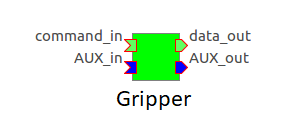
\includegraphics[width=0.4\linewidth]{fig/chp3/GripperDiag.png}
    \caption{Port configuration of RTC\_Gripper.}
    \label{fig:system:rtc-gripper}
\end{figure}

\paragraph{RTC\_Realsense}

RTC\_Realsenseは，librealsenseを用いてRealSense D435からカラー画像，赤外線画像，深度画像を取得し，RTC\_PointCloudProcessに送信するためのRTCである．
センサから取得したデータをRTCのデータ型に変換して出力するほか，深度画像から点群への変換，カラー画像の点群へのマッピング，深度画像のノイズ（librealsenseの内蔵フィルタ機能によるもので，\ref{sec:system:pointcloud:processing:pipeline}節で述べる点群処理パイプラインとは独立した前処理である）処理の各機能をRTC内に実装した．

データ処理とセンサ読込の速度差を吸収するため，各データチャネル（カラー，赤外線2系統，深度）にキューを設置した．
キューは常に最新データを末端に追加し，キューが満杯の際は最も古いデータ（先端）を破棄するリングバッファ方式とし，データ遅延を最小化するためキューサイズは5とした．
RTC\_Realsenseのポート構成を図\ref{fig:system:rtc-realsense}に示す．

\begin{figure}[ht]
    \centering
    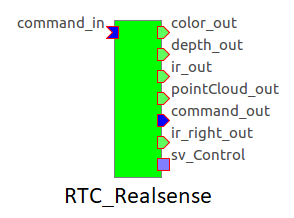
\includegraphics[width=0.4\linewidth]{fig/chp3/RealsenseDiag.png}
    \caption{Port configuration of RTC\_Realsense.}
    \label{fig:system:rtc-realsense}
\end{figure}

\paragraph{RTC\_PointCloudProcess}

RTC\_PointCloudProcessは，\ref{sec:system:software:pcl}節で述べたPCLを用いて，RTC\_Realsenseから受信した点群データを処理するRTCである．
処理の基本的な流れは以下の通りである：

\begin{enumerate}
    \item Pythonのメインスクリプトがサービスポートを通じて処理命令とパラメータをRTC\_PointCloudProcessに送信する．
    \item RTC\_PointCloudProcessがデータポートから点群を読み出す．
    \item \ref{sec:system:pointcloud:processing:pipeline}節で詳述するアルゴリズムにより点群を処理する．
    \item 処理結果をサービスポート経由でメインスクリプトに返す．
\end{enumerate}


RTC\_PointCloudProcessのポート構成を図\ref{fig:system:rtc-pointcloud-process}に，RTC全体の接続状況を図\ref{fig:system:rtc-overall-connections}に示す．

\begin{figure}[ht]
    \centering
    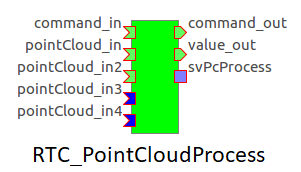
\includegraphics[width=0.4\linewidth]{fig/chp3/PointCloudProcessDiag.png}
    \caption{Port configuration of RTC\_PointCloudProcess.}
    \label{fig:system:rtc-pointcloud-process}
\end{figure}

\begin{figure}[ht]
    \centering
    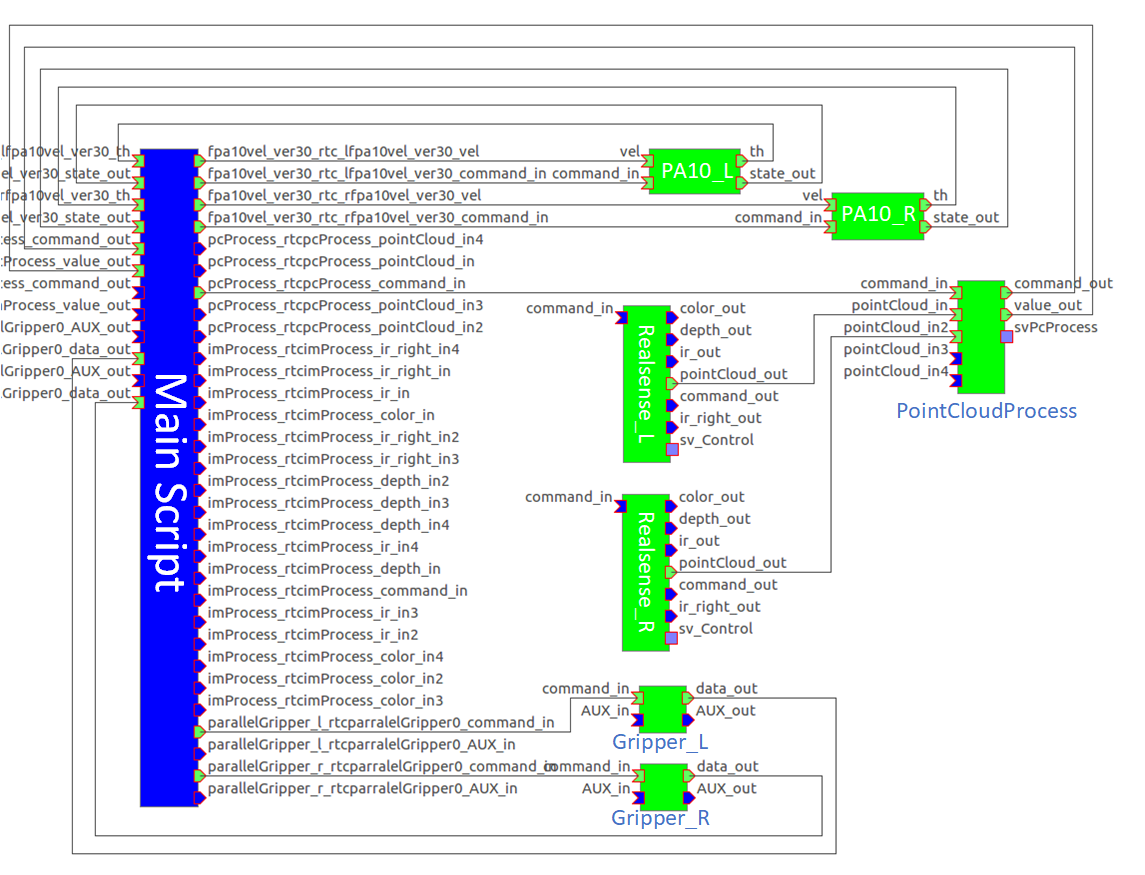
\includegraphics[width=0.9\linewidth]{fig/chp3/SystemDiag.png}
    \caption{Overall RTC connections.}
    \label{fig:system:rtc-overall-connections}
\end{figure}


\section{3D点群モデルの位置づけと全体パイプライン}
\label{sec:system:pointcloud:overview}

\subsection{本論文における点群モデルの役割}
\label{sec:system:pointcloud:role}
% TODO：RGB-Dカメラなどの深度センサにより非接触で取得可能である．这句话为什么要写？
\revise{本論文では，液体の注ぎ，食材の皮むき，および切断中の安定把持という三つの物体操作について，3次元点群モデルを共通の入力表現として用いる．}
点群モデルとは，対象物体表面の3次元座標点の集合であり，RGB-Dカメラなどの深度センサにより非接触で取得可能である．

具体的には，以下の各タスクにおいて点群モデルが中心的な役割を果たす：

\begin{enumerate}
  \item \textbf{食材の皮むき軌道生成}：皮むきタスクでは，食材表面の点群から法線ベクトルを計算し，皮むき軌道の事前生成および回転角度の算出に利用する．
  \item \textbf{容器の形状モデリング}：液体注ぎタスクでは，注ぐ容器および注ぎ先容器の内部形状を点群モデルとして取得し，容積計算することおよび液面高さから注いた量を計算するために用いる．
  \item \textbf{食材の表面形状取得}：食材把持タスクでは，食材の3次元形状を点群として取得し，把持位置探索のための幾何学的入力とする．
\end{enumerate}

これらのタスクに共通して，点群モデルは「対象物の幾何学的情報を計算機上で扱うための中間表現」として機能する．
点群表現を採用する理由は以下の通りである．
第一に，RGB-Dカメラの出力が深度画像（すなわちピクセル単位の3次元座標の集合）であり，点群表現がセンサ出力との親和性に最も優れること．
第二に，メッシュなどの表現と比較して，データ構造が単純であり，フィルタリング，ダウンサンプリング，領域分割といった処理の計算コストが低いこと．
第三に，容器の口縁検出，食材曲面追跡，把持点の探索などといった本研究が扱うタスクのいずれにおいても，物体表面の離散的なサンプリング点集合で十分な情報が得られることである．

各タスク固有の処理へ進む前に，共通する処理パイプラインを経由することで，後続のアルゴリズムへの入力品質を保証する設計となっている．

\subsection{点群取得・処理パイプラインの概要}
\label{sec:system:pointcloud:pipeline-overview}
本論文における3D点群モデル取得の共通処理パイプラインを図\ref{fig:system:pointcloud-pipeline}に示す．
パイプラインは大きく「点群取得」と「点群処理」の2段階に分けられる．

\begin{figure}[t]
  \centering
  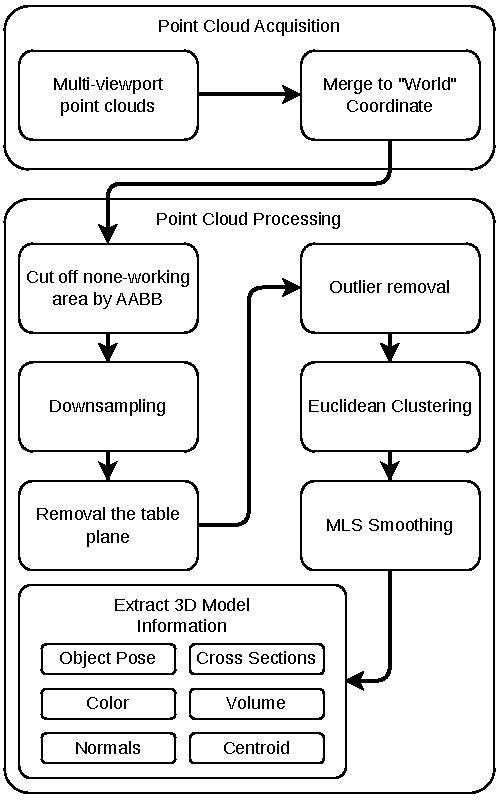
\includegraphics[width=0.6\linewidth]{fig/chp3/chp3_algo_flowchart.drawio.pdf}
  \caption{The pipeline for 3D point cloud model acquisition.}
  \label{fig:system:pointcloud-pipeline}
\end{figure}

\textbf{点群取得}では，RGB-Dカメラを用いて多視点から撮影した点群を，座標変換により合成し，対象物体の全周的な3次元形状を復元する．
この段階では，カメラキャリブレーション，座標系定義，多視点合成が主要な処理となる．

\textbf{点群処理}では，合成された点群に対して，作業領域の切り出し，ダウンサンプリング，作業台平面の除去，外れ値除去，クラスタリング，平滑化および法線ベクトル推定を順次適用し，後段のタスクに適した点群モデルを生成する．
この処理順序には必然性がある．
まず粗い空間フィルタ（作業領域切り出し）で計算負荷を低減し，次に密度均一化（ダウンサンプリング）により，この後の処理のパラメータは点群データの密度に依存させずに設定可能とする．
その上でテーブル平面除去，統計的なノイズ除去（外れ値除去），クラスタリングを経て，最後に表面の平滑化と法線推定を行う．

\section{3D点群モデルの取得}
\label{sec:system:pointcloud:acquisition}

\subsection{RGB-Dカメラによる点群取得}
\label{sec:system:pointcloud:acquisition:rgbd}
\ref{sec:system:hardware:vision-sensor}節で述べたRGB-Dカメラ（Intel RealSense D435）を用いて，対象物体の点群を撮影する．
本サブセクションでは，深度画像から3次元点群への変換メカニズムを述べる．

RealSense D435はアクティブステレオ方式により深度情報を取得し，RGB画像と深度画像を同時に出力する．
得られた深度画像とカメラ内部パラメータ（焦点距離 $f_x, f_y$，光学中心 $c_x, c_y$）から，ピンホールカメラモデルに基づく逆投影により，各ピクセルの3次元座標を計算する：

\begin{equation}
  \begin{bmatrix} X_C \\ Y_C \\ Z_C \end{bmatrix}
  = d \cdot
  \begin{bmatrix}
    \frac{1}{f_x} & 0 & -\frac{c_x}{f_x} \\
    0 & \frac{1}{f_y} & -\frac{c_y}{f_y} \\
    0 & 0 & 1
  \end{bmatrix}
  \begin{bmatrix} u \\ v \\ 1 \end{bmatrix}
  \label{eq:system:back_projection}
\end{equation}

ここで，$(u, v)$ は画像座標，$d$ は対応する深度値，$(X_C, Y_C, Z_C)$ はカメラ座標系 $\Sigma_C$ における3次元座標である．
カメラ座標系の原点はカメラの光学中心，$Z_C$ 軸は光学軸方向に設定する．

RGB-Dカメラの単一視点からの撮影では，対象物体の自己遮蔽や環境遮蔽により不可視となる領域が生じる．
このため，ロボットアームを動作させてカメラ姿勢を変更し，複数視点から点群を取得する必要がある．



\subsection{座標変換と多視点点群の合成}
\label{sec:system:pointcloud:acquisition:multi-view-fusion}
複数視点からの点群を合成する手順を以下に示す：

\begin{enumerate}
  \item ロボットアームを制御し，カメラが対象物体を取り囲むように複数の姿勢へ移動させる．
  \item 各姿勢においてRGB-Dカメラで点群を撮影し，カメラ座標系での点群 $\mathcal{P}_{C}^{(i)}$ を得る．
  \item 式(\ref{eq:system:transform_chain})に従い，各カメラ座標系の点群を世界座標系へ変換する：
  \begin{equation}
    \mathcal{P}_{W}^{(i)} = \left\{ {}^{W}\bm{T}_{H}^{(i)} \cdot {}^{H}\bm{T}_{C} \cdot \bm{p} \;|\; \bm{p} \in \mathcal{P}_{C}^{(i)} \right\}
  \end{equation}
  \item 全視点の点群を合成し，1つの点群 $\mathcal{P}_{\mathrm{all}}$ を得る：
  \begin{equation}
    \mathcal{P}_{\mathrm{all}} = \bigcup_{i=1}^{N_v} \mathcal{P}_{W}^{(i)}
  \end{equation}
  ここで，$N_v$ は視点数である．
\end{enumerate}

多視点合成により，対象物体の全周的な点群モデルが得られるが，重複領域の密度が不均一になる点や，位置姿勢誤差の蓄積による多重像が生じる点に留意する必要がある．

% \subsection{底面点群の取得}
% \label{sec:system:pointcloud:acquisition:bottom-surface}
% \paragraph{本章における位置づけ}

% 前節で述べた多視点点群合成処理により，対象物体のほぼ全周的な3次元形状が取得される．
% しかし，机上に置かれた物体を上方および側方からスキャンする構成では，底面（作業台との接触面付近）は不可視領域となる．
% 本節では，ロボットの把持機能を活用して物体を持ち上げ，底面を含む全周点群を取得する手法について述べる．

% \paragraph{卓上スキャンにおける不可視領域}

% 図\ref{fig:system:occlusion}に示すように，作業台上に静置された物体をRGB-Dカメラで多視点からスキャンしても，物体底面および作業台との接触部近傍の点群は原理的に取得不可能である．
% この不可視領域は，以下に起因する：

% \begin{enumerate}
%   \item 物体と作業台の接触による物理的遮蔽
%   \item カメラの俯角限界（アームの可動範囲制約）
%   \item 物体側面のオーバーハング形状による自己遮蔽
% \end{enumerate}

% \begin{figure}[t]
%   \centering
%   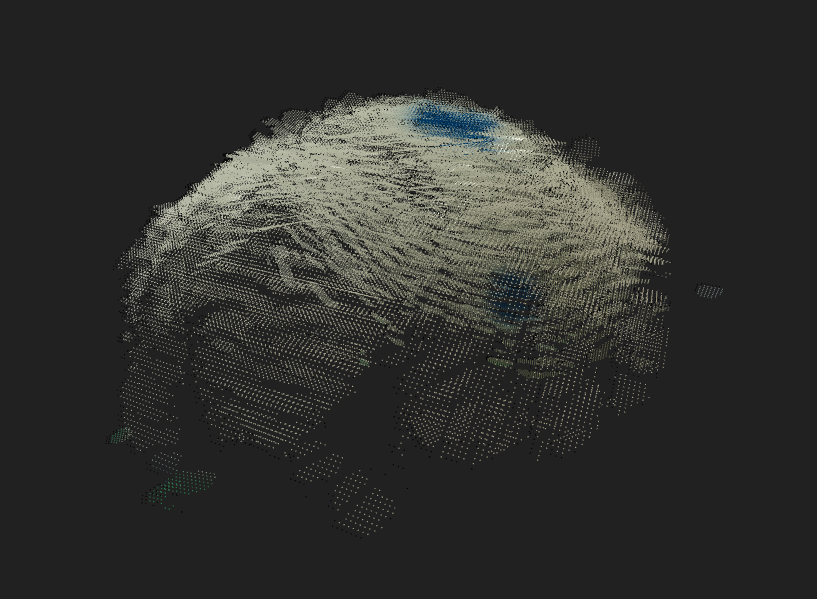
\includegraphics[width=0.70\linewidth]{fig/chp3/pointalgo_occlusion.png}
%   \caption{Invisible region in tabletop scanning.}

%     \label{fig:system:occlusion}
% \end{figure}

% % 底面情報の欠落は，特に容器の体積計算精度に重大な影響を及ぼす．
% % 例えば，深くて細い容器では底面付近の形状復元が不完全となるため，式(\ref{eq:volume_integral})の積分下限付近の誤差が累積し，全体の体積誤差が増大する．

% \paragraph{計算}

% ロボットハンドにより物体を把持して持ち上げた状態で，物体底面をカメラで撮影する．
% このとき，把持後の物体は手先座標系に対して固定されているため，撮影された底面点群は以下の座標変換により世界座標系の既存点群と合成される：

% \begin{equation}
%   \mathcal{P}_{\mathrm{bottom}}^{(W)} = \left\{ {}^{W}\bm{T}_{H}^{(g)} \cdot {}^{H}\bm{T}_{C} \cdot \bm{p} \;|\; \bm{p} \in \mathcal{P}_{\mathrm{bottom}}^{(C)} \right\}
%   \label{eq:system:bottom_transform}
% \end{equation}

% ここで，${}^{W}\bm{T}_{H}^{(g)}$ は底面撮影時のロボット手先の順運動学解，$\mathcal{P}_{\mathrm{bottom}}^{(C)}$ はカメラ座標系における底面点群である．

% 既存の点群モデル $\mathcal{P}_{\mathrm{obj}}$ と底面点群 $\mathcal{P}_{\mathrm{bottom}}^{(W)}$ の合成は，ICP（Iterative Closest Point）アルゴリズムによる精密位置合わせの後に実施する：

% \begin{equation}
%   \mathcal{P}_{\mathrm{full}} = \mathcal{P}_{\mathrm{obj}} \cup \mathcal{P}_{\mathrm{bottom}}^{(W, \mathrm{aligned})}
%   \label{eq:system:full_model}
% \end{equation}

% \paragraph{手順}

% 把持を利用した底面点群取得の手順を以下に示す：

% \begin{enumerate}
%   \item \textbf{三指把持による対象物の持ち上げ}：
%   事前に計画された把持位置に基づき，ロボットハンドの3指で対象物体を把持し，作業台から十分な高さ（約150\,mm）まで持ち上げる．
%   持ち上げ高さは，カメラの最小撮影距離と作業台の映り込み回避を考慮して決定する．

%   \item \textbf{底面点群の撮影と座標変換}：
%   持ち上げ状態で，カメラを物体の下方に向け，底面の点群を撮影する．
%   必要に応じてハンドのリストロール軸を回転させ，複数の底部視点を取得する．
%   撮影された各底面点群は，式(\ref{eq:system:bottom_transform})により世界座標系へ変換する．

%   \item \textbf{既存点群との位置合わせと合成}：
%   底面点群と既存の物体点群モデルの重複領域（側面下部）を用いてICPによる精密位置合わせを行う．
%   位置合わせ後，式(\ref{eq:system:full_model})により両者を合成し，底面を含む完全な物体モデルを生成する．
% \end{enumerate}

\subsection{底面点群の取得}
\label{sec:system:bottom_acquisition}

\ref{sec:system:pointcloud:acquisition:multi-view-fusion}節で述べた多視点合成により，対象物の上面および側面の大部分は取得できる．
しかし，対象物が作業台上に置かれている限り，作業台との接触面およびその近傍は，カメラ視線が到達しない不可視領域として残る．
この欠落は，対象物の外表面点群を全周モデルとして扱う処理に影響する．
\revise{卓上スキャンのみで得られる点群は，上面および側面のみの観測であり，底面側の点，法線，および外形の完全性が欠落する．}
そのため，食材や不定形物体の外形モデルを用いた把持候補生成，幾何学的重心の近似，および外形再構成精度の評価では，観測方向に依存した偏りが生じる可能性がある．
\begin{revisionblock}
この問題に対し，本研究では対象物を把持して作業台から持ち上げ，底面側を観測可能な状態へ能動的に変換した後，複数の提示姿勢で点群を取得する．
平面上に置かれた不規則形状物体の下面は，卓上カメラの視点数を増やすだけでは原理的に取得できない．
ロボットの把持動作を視点生成手段として利用し，持ち上げ前後の手先姿勢から点群を元の物体姿勢へ戻して統合する点は，後続タスクのための単なる前処理にとどまらず，不可視面を補完する本研究の計測上の寄与である．
\end{revisionblock}
% 本手法のポイントは，対象物を把持して提示姿勢を変化させるだけでなく，同一の把持姿勢および同一の提示姿勢列に対して，ハンドのみの点群と対象物を含む点群を対で取得する点にある．
% これにより，ロボットハンドのCADモデルを明示的に用いずに，観測点群からハンド領域を除去し，対象物表面のみを抽出できる．


% \subsubsection{底面点群取得の方針}
% \label{sec:system:bottom_acquisition_policy}

% テーブル上に置いた物体を上および側面から撮影する方法では，物体とテーブル平面が接触しているため，底面は観測できない領域として残る．
% 本研究では，この観測できない領域を補完するため，対象物をサーボハンドで把持してテーブル平面から持ち上げ，底面側をRGB-Dカメラから観測可能な状態にする．
% % TODO:少了一句核心的复原到底面位置，删除手指才是顺带的．
% ただし，持ち上げた状態で取得した点群には，対象物だけでなくサーボハンドも含まれる．
% そのため，本手法では，サーボハンドのみを撮影した点群を用いてハンド領域を除去し，得られた底面側点群をテーブル上に置かれていたときの姿勢へ復元する．

% 本節では，点群を以下の三種類に分けて扱う．
% テーブル上に置いた物体の可視部分の点群を$\mathcal{P}_{\mathrm{top}}$，対象物を持ち上げた姿勢で取得した底面側の点群を${}^{}\mathcal{P}_{\mathrm{bot1}}$，それをテーブル上の姿勢へ復元した点群を$\mathcal{P}_{\mathrm{bot2}}$と表す．

% この復元では，把持中に対象物とロボットの手先の相対姿勢が変化しないと仮定する．
% すなわち，対象物の点群は，ロボットの手先座標系$\Sigma_H$から見ると同じ位置にあるとみなす（すなわち，${}^{H1}\mathcal{P}_{\mathrm{bot1}}={}^{H2}\mathcal{P}_{\mathrm{bot2}}$）．
% この仮定に基づき，持ち上げた姿勢で得られた底面側点群を，ロボットの手先姿勢を用いてテーブル上の姿勢へ変換する．

% \subsubsection{底面点群取得の処理の流れ}
% \label{sec:system:bottom_acquisition_flow}

% \paragraph{把持の関節角度の記録}
% まず，対象物をテーブル上に置いた状態でサーボハンドを閉じ，対象物に安定接触（末端サーボのトルクが閾値以上）した時点の各サーボ関節の角度を保存する．
% 対象物なしでサーボハンドのみを撮影する場合と，対象物を把持して撮影する場合とで同じ把持の関節角度を用いることで，ハンド形状をできるだけ一致させる．
% また，このときのロボットの手先姿勢を，テーブル上の基準姿勢として記録する．
% この手先姿勢を${}^{W}\bm{T}_{H2}^{\mathrm{}}$とする．
% ここで，${}^{W}\bm{T}_{H2}^{\mathrm{}}$はテーブル上の基準姿勢における手先座標系から世界座標系への変換である．

% \paragraph{可視部分${}^{W}\mathcal{P}_{\mathrm{top}}$の取得}
% 次に，対象物をテーブル上に置いた状態で，上方および側方から撮影を行い，可視部分の点群${}^{W}\mathcal{P}_{\mathrm{top}}$を取得する．
% % この点群には，上面および側面の多くが含まれる一方で，底面およびテーブル平面との接触部近傍は含まれない．

% \paragraph{底面側点群の取得}
% 続いて，保存した把持の関節角度を用いて対象物を把持し，テーブル平面から持ち上げる．
% この状態で，RGB-Dカメラにより底面および下部側面を撮影する．
% 得られた点群は，\ref{sec:system:camera_calibration}節で述べたカメラ外部パラメータと撮影時のロボット姿勢に基づき，世界座標系へ変換される．
% この点群を${}^{W}\mathcal{P}_{\mathrm{bot1}}$とする．
% また，この撮影時の手先姿勢を${}^{W}\bm{T}_{H}^{\mathrm{lift}}$とする．

% \paragraph{ハンド領域の除去}
% 持ち上げ状態で取得した点群には，対象物表面だけでなくサーボハンド表面の点も含まれる．
% そこで，同じ把持の関節角度を対象物なしで再現し，サーボハンドのみの点群を取得する．
% 対象物を把持した点群とサーボハンドのみの点群は，同じ手先姿勢および同じ把持の関節角度で取得されるため，サーボハンド表面に対応する点はほぼ同じ空間位置に現れる．
% このため，対象物を把持した点群のうち，サーボハンドのみの点群に近い点をハンド領域として除去する．
% この処理により，サーボハンドのCADモデルを用いずに，底面側の対象物点群${}^{W}\mathcal{P}_{\mathrm{bot1}}$を抽出する．

% \paragraph{テーブル上の姿勢への復元と統合}
% ${}^{W}\mathcal{P}_{\mathrm{bot1}}$は世界座標系で表されているが，対象物は持ち上げられた姿勢にある．
% したがって，この点群をそのまま${}^{W}\mathcal{P}_{\mathrm{top}}$に加えることはできない．
% そこで，把持中に対象物と手先座標系$\Sigma_H$との相対姿勢が変化しないという仮定に基づき，${}^{W}\mathcal{P}_{\mathrm{bot1}}$をテーブル上の姿勢へ復元する．

% 持ち上げ状態で観測された底面側の点を${}^{W}\bm{p}_{\mathrm{bot1}}$，テーブル上の姿勢へ復元した点を${}^{W}\bm{p}_{\mathrm{bot2}}$とすると，両者の関係は次式で表される．

% % \begin{equation}
% %   {}^{W}\bm{p}_{\mathrm{bot2}}
% %   =
% %   {}^{W}\bm{T}_{H}^{\mathrm{table}}
% %   \left(
% %     {}^{W}\bm{T}_{H}^{\mathrm{lift}}
% %   \right)^{-1}
% %   {}^{W}\bm{p}_{\mathrm{bot1}}
% %   \label{eq:system:bottom_restore_point}
% % \end{equation}
% \begin{equation}
% \begin{aligned}
%   {}^{W}\bm{p}_{\mathrm{bot2}}
%   &=
%   {}^{W}\bm{T}_{H2}
%   \,
%   {}^{H2}\bm{p}_{\mathrm{bot2}}
%   \\
%   &=
%   {}^{W}\bm{T}_{H2}
%   \,
%   {}^{H1}\bm{p}_{\mathrm{bot1}}
%   \\
%   &=
%   {}^{W}\bm{T}_{H2}
%   \,
%   {}^{H1}\bm{T}_{W}
%   \,
%   {}^{W}\bm{p}_{\mathrm{bot1}}
% \end{aligned}
% \label{eq:system:bottom_restore_point}
% \end{equation}

% この式は，持ち上げ状態の点を一度手先座標系$\Sigma_H$へ戻し，その後，テーブル上の基準姿勢における手先姿勢へ変換することを表す．
% 式\ref{eq:system:bottom_restore_point}の1-2行の${}^{H1}\mathcal{P}_{\mathrm{bot1}}$を${}^{H2}\mathcal{P}_{\mathrm{bot2}}$に入れ替われるのは\ref{sec:system:bottom_acquisition_policy}節最後の段落の${}^{H1}\mathcal{P}_{\mathrm{bot1}}={}^{H2}\mathcal{P}_{\mathrm{bot2}}$の仮定です．

% 最後に，上方および側方から撮影して得られた可視部分${}^{W}\mathcal{P}_{\mathrm{top}}$と，テーブル上の姿勢へ復元された底面側点群${}^{W}\mathcal{P}_{\mathrm{bot2}}$を統合する．

% \begin{equation}
%   {}^{W}\mathcal{P}_{\mathrm{full}}
%   =
%   {}^{W}\mathcal{P}_{\mathrm{top}}
%   \cup
%   {}^{W}\mathcal{P}_{\mathrm{bot2}}
%   \label{eq:system:bottom_full_cloud}
% \end{equation}

% ここで得られる${}^{W}\mathcal{P}_{\mathrm{full}}$は，テーブル上に置いた状態で観測できる上面・側面点群に，持ち上げ撮影によって得られた底面および下部側面を加えた外表面点群である．
% この点群は，対象物外形の補完，法線推定，幾何学的重心の近似，および把持候補生成のために用いる．




















\subsubsection{底面点群取得の方針}
\label{sec:system:bottom_acquisition_policy}

テーブル上に置いた物体を上方および側方から撮影する方法では，物体とテーブル平面が接触しているため，底面は観測できない領域として残る．
本研究では，この観測できない領域を補完するため，対象物をサーボハンドで把持してテーブル平面から持ち上げ，底面側をRGB-Dカメラから観測可能な状態にする．
本手法の中心は，持ち上げた姿勢で得られた底面側点群を，ロボットの手先姿勢の変化に基づいて，物体がテーブル上に置かれていたときの姿勢へ復元する点にある．
ただし，持ち上げた状態で取得した点群には対象物だけでなくサーボハンドも含まれるため，復元の前にサーボハンドに由来する点を除去する．

本節では，点群を以下の三種類に分けて扱う．
テーブル上に置いた物体の可視部分の点群を${}^{W}\mathcal{P}_{\mathrm{top}}$，対象物を持ち上げた姿勢で取得した底面側の点群を${}^{W}\mathcal{P}_{\mathrm{bot1}}$，それをテーブル上の姿勢へ復元した点群を${}^{W}\mathcal{P}_{\mathrm{bot2}}$と表す．
左上の$W$は，点群が世界座標系$\Sigma_W$で記述されていることを示す．
また，持ち上げ撮影時の手先座標系を$\Sigma_{H_1}$，テーブル上の基準姿勢における手先座標系を$\Sigma_{H_2}$とする．

復元では，把持中に対象物とロボットの手先の相対姿勢が変化しないと仮定する．
したがって，同じ対象物表面点は，$\Sigma_{H_1}$から見ても$\Sigma_{H_2}$から見ても同じ手先座標値を持つとみなせる．
この関係を用いて，持ち上げ姿勢で得られた${}^{W}\mathcal{P}_{\mathrm{bot1}}$を，テーブル上の姿勢に対応する${}^{W}\mathcal{P}_{\mathrm{bot2}}$へ変換する．

\subsubsection{底面点群取得の処理の流れ}
\label{sec:system:bottom_acquisition_flow}

\paragraph{把持の関節角度と基準姿勢の記録}
まず，対象物をテーブル上に置いた状態でサーボハンドを閉じ，対象物に安定接触した時点の各サーボ関節の角度を保存する．
ここで保存する把持の関節角度は，対象物なしでサーボハンドのみを撮影する場合と，対象物を把持して撮影する場合とで，ハンド形状を一致させるために用いる．
また，このときのロボットの手先姿勢を，テーブル上の基準姿勢として記録する．
この手先姿勢を${}^{W}\bm{T}_{H_2}$とする．
ここで，${}^{W}\bm{T}_{H_2}$は，テーブル上の基準姿勢における手先座標系$\Sigma_{H_2}$から世界座標系$\Sigma_W$への変換である．

\paragraph{可視部分${}^{W}\mathcal{P}_{\mathrm{top}}$の取得}
次に，対象物をテーブル上に置いた状態で，上方および側方から撮影を行い，可視部分の点群${}^{W}\mathcal{P}_{\mathrm{top}}$を取得する．
この点群には，物体の上面および側面が含まれるが，底面およびテーブル平面との接触部近傍は含まれない．

\paragraph{底面側点群の取得}
続いて，保存した把持の関節角度を用いて対象物を把持し，テーブル平面から持ち上げる．
この状態で，RGB-Dカメラにより底面および下部側面を撮影する．
得られた点群は，\ref{sec:system:camera_calibration}節で述べたカメラ外部パラメータと撮影時のロボット姿勢に基づき，世界座標系へ変換される．
また，この撮影時の手先姿勢を${}^{W}\bm{T}_{H_1}$とする．
ここで，${}^{W}\bm{T}_{H_1}$は，持ち上げ撮影時の手先座標系$\Sigma_{H_1}$から世界座標系$\Sigma_W$への変換である．

\paragraph{ハンド領域の除去}
持ち上げ状態で取得した点群には，対象物表面だけでなくサーボハンド表面の点も含まれる．
そこで，同じ把持の関節角度を対象物なしで再現し，サーボハンドのみの点群を取得する．
対象物を把持した点群のうち，サーボハンドのみの点群に近い点をハンド領域として除去し，残った点群を持ち上げ姿勢における底面側点群${}^{W}\mathcal{P}_{\mathrm{bot1}}$とする．
この処理により，サーボハンドのCADモデルを用いずに，対象物の底面側点群を抽出できる．

\paragraph{テーブル上の姿勢への復元と統合}
${}^{W}\mathcal{P}_{\mathrm{bot1}}$は世界座標系で表されているが，対象物は持ち上げられた姿勢にある．
したがって，この点群をそのまま${}^{W}\mathcal{P}_{\mathrm{top}}$に加えることはできない．
そこで，手先姿勢${}^{W}\bm{T}_{H_1}$および${}^{W}\bm{T}_{H_2}$を用いて，${}^{W}\mathcal{P}_{\mathrm{bot1}}$をテーブル上の姿勢へ復元する．

持ち上げ状態で観測された底面側の点を${}^{W}\bm{p}_{\mathrm{bot1}}$，テーブル上の姿勢へ復元した点を${}^{W}\bm{p}_{\mathrm{bot2}}$とすると，両者の関係は次式で表される．

\begin{equation}
\begin{aligned}
  {}^{W}\bm{p}_{\mathrm{bot2}}
  &=
  {}^{W}\bm{T}_{H_2}
  \,
  {}^{H_2}\bm{p}_{\mathrm{bot2}}
  \\
  &=
  {}^{W}\bm{T}_{H_2}
  \,
  {}^{H_1}\bm{p}_{\mathrm{bot1}}
  \\
  &=
  {}^{W}\bm{T}_{H_2}
  \left(
    {}^{W}\bm{T}_{H_1}
  \right)^{-1}
  {}^{W}\bm{p}_{\mathrm{bot1}}
\end{aligned}
\label{eq:system:bottom_restore_point}
\end{equation}

式\eqref{eq:system:bottom_restore_point}の1行目は，復元後の点${}^{W}\bm{p}_{\mathrm{bot2}}$を，テーブル上の基準姿勢における手先座標${}^{H_2}\bm{p}_{\mathrm{bot2}}$から世界座標系へ変換することを表す．
2行目では，把持中に対象物と手先の相対姿勢が変化しないという仮定を用い，${}^{H_2}\bm{p}_{\mathrm{bot2}}$を持ち上げ撮影時の手先座標${}^{H_1}\bm{p}_{\mathrm{bot1}}$に置き換えている．
3行目では，持ち上げ状態で世界座標系に表されている点${}^{W}\bm{p}_{\mathrm{bot1}}$を，$\left({}^{W}\bm{T}_{H_1}\right)^{-1}$により手先座標系$\Sigma_{H_1}$へ変換している．
したがって，式\eqref{eq:system:bottom_restore_point}は，持ち上げ状態の底面側点群を一度手先座標系へ戻し，その後，テーブル上の基準姿勢における手先姿勢へ写す変換である．

点群全体に式\eqref{eq:system:bottom_restore_point}を適用することで，テーブル上の姿勢へ復元された底面側点群${}^{W}\mathcal{P}_{\mathrm{bot2}}$を得る．
最後に，上方および側方から撮影して得られた可視部分${}^{W}\mathcal{P}_{\mathrm{top}}$と，復元された底面側点群${}^{W}\mathcal{P}_{\mathrm{bot2}}$を統合する．

\begin{equation}
  {}^{W}\mathcal{P}_{\mathrm{full}}
  =
  {}^{W}\mathcal{P}_{\mathrm{top}}
  \cup
  {}^{W}\mathcal{P}_{\mathrm{bot2}}
  \label{eq:system:bottom_full_cloud}
\end{equation}

ここで得られる${}^{W}\mathcal{P}_{\mathrm{full}}$は，テーブル上に置いた状態で観測できる上面・側面点群に，持ち上げ撮影によって得られた底面および下部側面を加えた外表面点群である．
この点群は，対象物外形の補完，法線推定，幾何学的重心の近似，および把持候補生成のために用いる．








































\section{3D点群モデルの処理}
\label{sec:system:pointcloud:processing}

\subsection{処理パイプライン}
\label{sec:system:pointcloud:processing:pipeline}

合成後の点群 $\mathcal{P}_{\mathrm{all}}$ には，対象物体以外の点（作業台，背景，センサノイズなど）が含まれるため，以下の処理パイプラインを適用して対象物体の点群モデルを抽出する．
% 本処理は，表\ref{tab:system:configuration-diff}に示したいずれのアーキテクチャにおいても同一のアルゴリズムを用いて実装した（PCL\cite{PCL}，Open3D，または自作PCL-Pythonラッパー経由）．

\paragraph{作業領域の切り出し}

まず，ロボットの作業範囲外の不要な点を除去するため，世界座標系における3次元矩形領域（Axis-Aligned Bounding Box; AABB）を指定し，領域外の点をフィルタリングする．
具体的には，作業台上面を基準とした $x, y, z$ 各軸方向の範囲 $[x_{\min}, x_{\max}] \times [y_{\min}, y_{\max}] \times [z_{\min}, z_{\max}]$ を経験的に設定し，Pass-Throughフィルタを適用する．

\begin{equation}
  \mathcal{P}_{\mathrm{roi}} = \left\{ \bm{p} \in \mathcal{P}_{\mathrm{all}} \;|\; \bm{p} \in [x_{\min}, x_{\max}] \times [y_{\min}, y_{\max}] \times [z_{\min}, z_{\max}] \right\}
  \label{eq:system:roi}
\end{equation}

これにより，後段処理の計算負荷が低減されるとともに，背景領域の誤検出が抑制される．

\paragraph{ダウンサンプリング}

多視点合成後の点群は高密度であり，後段の処理を効率化するため，Voxel Gridフィルタを用いてダウンサンプリングを行う．

Voxel Gridフィルタでは，3次元空間を一辺 $l_v$ のボクセル格子に分割し，各ボクセル内の点群をその重心位置で代表する：

\begin{equation}
  \mathcal{P}_{\mathrm{ds}} = \left\{ \frac{1}{|\mathcal{V}_k|} \sum_{\bm{p} \in \mathcal{V}_k} \bm{p} \;|\; \mathcal{V}_k \neq \emptyset \right\}
\end{equation}

ここで，$\mathcal{V}_k$ は $k$ 番目のボクセルに含まれる点の集合，$|\mathcal{V}_k|$ はその点数を表す．
本論文では，ボクセルサイズ $l_v = 1.0$\,mm を基本値とし，タスクに応じて調整する．
ダウンサンプリングにより，点群の密度が均一化され，かつ計算量が大幅に削減される．

\paragraph{作業台平面の除去}

作業領域内には，対象物体に加えて作業台平面が含まれている．
作業台平面は Random Sample Consensus（RANSAC）\cite{PCL-RANSAC} を用いて検出・除去する．

RANSACによる平面検出では，以下の処理を反復する：
% TODO: 3点？PCL是这样么
\begin{enumerate}
  \item 点群から3点をランダムに選択し，それらが定義する平面モデル $ax + by + cz + d = 0$ を生成する．
  \item 全点に対して，平面モデルからの距離が閾値 $\epsilon_p$ 以内の点をインライアとして集計する．
  \item 十分な反復回数の後，最多のインライア数を得た平面モデルを採用する．
\end{enumerate}

採用された平面モデルに対するインライア点を点群から除去することで，作業台平面を除外する：

\begin{equation}
  \mathcal{P}_{\mathrm{noplanar}} = \mathcal{P}_{\mathrm{ds}} \setminus \left\{ \bm{p} \in \mathcal{P}_{\mathrm{ds}} \;|\; \mathrm{dist}(\bm{p}, \Pi) \leq \epsilon_p \right\}
  \label{eq:system:plane_removal}
\end{equation}

ここで，$\Pi$ は検出された平面，$\mathrm{dist}(\bm{p}, \Pi)$ は点 $\bm{p}$ と平面 $\Pi$ の直交距離である．
本論文では $\epsilon_p = 2.0$\,mm を用いた．

\paragraph{外れ値除去}

センサノイズや多重像に起因する疎な外れ値点を除去するため，Statistical Outlier Removalフィルタを適用する．
本フィルタでは，各点について $k$ 近傍点までの平均距離 $\bar{d}_i$ を計算し，全点の平均距離分布に基づいて外れ値を判定する：

\begin{equation}
  \mathcal{P}_{\mathrm{filtered}} = \left\{ \bm{p}_i \in \mathcal{P}_{\mathrm{noplanar}} \;|\; \bar{d}_i \leq \mu_d + \alpha \sigma_d \right\}
\end{equation}

ここで，$\mu_d$ は全点の近傍平均距離の平均，$\sigma_d$ は標準偏差，$\alpha$ は許容度パラメータである．
本研究では $k = 50$，$\alpha = 1.0$ を標準的に用いる．

また，PCLに実装されているRadius Outlier Removal\cite{PCL-method}も併用し，半径 $r_r$ 内に存在する近傍点数が閾値 $n_{\min}$ 未満の点を孤立点として除去する．

\paragraph{クラスタリングによる対象物抽出}

平面除去および外れ値除去後の点群には，対象物体に加えて作業台上の他の物体や残留ノイズが含まれる可能性がある．
そこで，Euclidean Clustering\cite{PCL-method}を適用し，空間的に連続する点群を個別のクラスタに分割する．

Euclidean Clusteringでは，点間のユークリッド距離が閾値 $d_{\mathrm{th}}$ 未満の場合に同一クラスタとみなす：

\begin{equation}
  \mathrm{cluster}(\bm{p}_i, \bm{p}_j) = \begin{cases}
    \text{同じクラスタ} & \text{if } \|\bm{p}_i - \bm{p}_j\| \leq d_{\mathrm{th}} \\
    \text{異なるクラスタ} & \text{otherwise}
  \end{cases}
\end{equation}

各クラスタに対して，点数 $N_{\mathrm{cluster}}$ および重心位置の評価により対象物体を同定する．
具体的には，閾値 $N_{\min}$ 以上の点数を有し，かつ重心が作業領域内の適切な位置にあるクラスタを対象物体の点群 $\mathcal{P}_{\mathrm{obj}}$ として選択する．

\paragraph{平滑化と法線ベクトル推定}

クラスタリングにより抽出された対象物体の点群 $\mathcal{P}_{\mathrm{obj}}$ に対し，Moving Least Squares（MLS）法\cite{PCL-MLS}による平滑化と法線ベクトル推定を同時に適用する．

MLS法では，各点 $\bm{p}_i$ の近傍点群に対して局所的な多項式曲面をフィッティングし，再サンプリングすることで平滑化された点群 $\mathcal{P}_{\mathrm{smooth}}$ を得る．
同時に，フィッティングされた局所曲面の法線方向として，各点の法線ベクトル $\bm{n}_i$ が計算される：

\begin{equation}
  \bm{n}_i = \frac{\partial \mathcal{S}}{\partial x} \times \frac{\partial \mathcal{S}}{\partial y} \Big|_{\bm{p}_i}
\end{equation}

ここで，$\mathcal{S}$ は局所近似曲面である．
法線ベクトルは，後段のタスク（把持位置探索，皮むき軌道生成，表面領域分割など）において必須の幾何学情報となる．

なお，MLS法の局所近似半径 $r_{\mathrm{mls}}$ は，点群密度に依存するパラメータであり，本研究では経験的に $r_{\mathrm{mls}} = 3.0$\,mm を用いる．

\subsection{点群処理パラメータ}
\label{sec:system:pointcloud:processing:parameters}
表\ref{tab:system:pointcloud-parameters}に，本章で用いる標準的な点群処理パラメータをまとめる．
これらの値は，使用するRGB-Dカメラの特性，対象物体のサイズ，および作業環境に応じて調整される．

\begin{table}[t]
  \centering
  \caption{Standard parameters for point cloud processing.}
  \label{tab:system:pointcloud-parameters}
  \begin{tabular}{lcl}
    \toprule
    \textbf{Processing step} & \textbf{Parameter} & \textbf{Standard value} \\
    \midrule
    Voxel Grid downsampling & Voxel size $l_v$ & 1.0\,mm \\
    RANSAC plane removal & Distance threshold $\epsilon_p$ & 2.0\,mm \\
    Statistical Outlier Removal & Number of neighbors $k$ & 50 \\
    Statistical Outlier Removal & Tolerance $\alpha$ & 1.0 \\
    Radius Outlier Removal & Search radius $r_r$ & 5.0\,mm \\
    Radius Outlier Removal & Minimum number of neighbors $n_{\min}$ & 10 \\
    Euclidean Clustering & Cluster distance threshold $d_{\mathrm{th}}$ & 3.0\,mm \\
    Euclidean Clustering & Minimum cluster size $N_{\min}$ & 500 \\
    MLS smoothing & Local approximation radius $r_{\mathrm{mls}}$ & 3.0\,mm \\
    \bottomrule
  \end{tabular}
\end{table}

\subsection{点群モデルから得られる基礎情報}
\label{sec:system:pointcloud:basic-information}
前処理を経て得られた点群モデル $\mathcal{P}_{\mathrm{obj}}$ から，後段のタスクを遂行するために以下の基礎情報が抽出される．

\paragraph{位置姿勢と範囲}

点群モデルのAABBや主成分を計算することにより，世界座標系における物体の位置姿勢や範囲を取得する．この情報は，ロボットアームの到達可能性判定，衝突回避，およびカメラの再撮影時の視点計画に利用される．

\paragraph{色情報}

RGB-Dカメラからは各点の3次元座標に加えて色情報（RGB値）が取得される．
色情報は主に特定色の抽出による対象領域を識別するために用いる．

\paragraph{法線ベクトル}

MLS平滑化により推定された法線ベクトル $\{ \bm{n}_i \}$ は，以下のタスクにおいて中心的役割を果たす：

\begin{enumerate}
  \item 把持位置の力学的評価（力の釣り合い解析の幾何学的入力）
  \item 物体表面の曲率評価
\end{enumerate}

% TODO：把第五章的断面面积的计算拿到这里

\paragraph{断面と体積計算}

物体の幾何学的特性を定量化するため，点群モデルから断面情報を抽出する．
容器モデルの場合，以下の手順で体積計算が可能である：

\begin{enumerate}
  \item 点群モデルを $z$ 軸方向に一定間隔 $\Delta h$（本論文では $\Delta h = 1$\,mm）でスライスする．
  \item 各スライス高さ $h_k$ において，スライス平面から閾値以内の点群を当該断面の点集合とする．
  \item 断面点群をスライス面に投影し，投影点群の凸包を Quickhull アルゴリズム\cite{PCL-Convex}により計算する．
  \item 凸包の面積 $A(h_k)$ を断面積として算出する．
  \item 全スライスの断面積を高さ方向に積分することで，任意の液面高さ $H$ までの体積 $V(H)$ を求める：
  \begin{equation}
    V(H) = \int_{0}^{H} A(h)\, dh \approx \sum_{k:\,h_k \leq H} A(h_k) \cdot \Delta h
    \label{eq:system:volume_integral}
  \end{equation}
\end{enumerate}

\revise{この断面積分法により，本研究で扱う開口容器について，個々の容器形状から体積を計算できる（図\ref{fig:system:cross-section}）．ただし，凹部や内部遮蔽によって内面点群が欠落する容器では近似誤差が生じる．}

\begin{figure}[t]
  \centering
  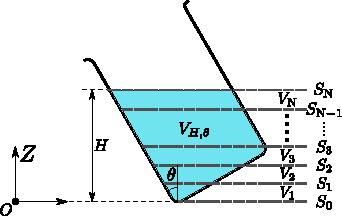
\includegraphics[width=0.75\linewidth]{fig/chp_pouring/ParametersV4.pdf}
  \caption{Conceptual diagram of point-cloud slicing and cross-sectional area calculation.}
  \label{fig:system:cross-section}
\end{figure}

\paragraph{重心}

物体の幾何学的重心 $\bm{g}$ は，点群の全点の座標平均として近似計算される：

\begin{equation}
  \bm{g} = \frac{1}{|\mathcal{P}_{\mathrm{obj}}|} \sum_{\bm{p} \in \mathcal{P}_{\mathrm{obj}}} \bm{p}
  \label{eq:system:centroid}
\end{equation}

重心位置は，把持の力学的安定性評価における重要な入力であり，特に食材把持タスクでは，食品の密度が比較的均一であるとの仮定の下，幾何学的重心を質量中心の近似値として使用する．

\paragraph{表面領域と指先位置候補}

点群モデルから，物体表面の各点を指先把持位置の候補として利用する．
具体的には，$\mathcal{P}_{\mathrm{obj}}$ の各点 $\bm{p}_i$ を指先位置候補とし，対応する法線ベクトル $\bm{n}_i$ を指先の接近方向として扱う．
これにより，多数の把持候補（最大で $K = |\mathcal{P}_{\mathrm{obj}}|$ 個）が生成される．
計算効率の観点から，事前に点群をダウンサンプリングして候補点数を制限する（例：実験では約150〜200点に制限）．

\paragraph{後続章における利用}

上記の基礎情報は，後続する各章において以下のように利用される：

\begin{enumerate}
  \item \textbf{第4章-皮むき作業}：物体表面の法線ベクトルに基づく皮むき軌道の事前生成，法線角度変化に基づく軌道セグメント化，および皮むきエッジの色情報抽出．
  \item \textbf{第5章-液体を注ぐ作業}：容器の断面積データを用いた注いだ体積計算，および液面検出のためのAABBによる領域制限．
  \item \textbf{第6章-切断時の安定把持}：表面点群を把持の探索空間とし，法線ベクトルと重心位置を用いた把持のスコア計算．
\end{enumerate}

% ============================================================
% TODO：通过程序生成


\section{3D点群モデル取得の精度評価実験}
\label{sec:system:pointcloud:evaluation}

本節では，前節までに述べた多視点点群取得，座標変換，点群処理，および基礎幾何情報抽出の精度を，実験により評価する．
本論文で用いる3D点群モデルは，後続章において皮むき軌道生成，容器容積計算，および把持点探索の入力となる．
したがって，評価では単に点群が見た目として対象物を再現できているかではなく，タスクで利用される幾何量がどの程度安定に得られるかを確認する必要がある．
この目的のため，本節では以下の三種類の実験を行った．
第一に，球および円柱という幾何学的形状が既知の標準物体を撮影し，プリミティブフィッティングにより得られる半径，軸方向，および位置の誤差を評価した．
第二に，3Dプリンタで作製した形状の異なる5種類の容器を撮影し，容積計算精度およびCADモデルに対する表面形状誤差を評価した．
第三に，卓上観測では欠落しやすい底面側の点群を把持・持ち上げによって補完する手法について，CADモデルとの距離誤差により評価した．

\subsection{評価指標}
\label{sec:system:pointcloud:evaluation:metrics}

本節の評価では，対象物と実験目的に応じて，プリミティブパラメータ誤差，点群から参照モデルへの距離誤差，および容積誤差を用いる．

\paragraph{プリミティブパラメータ誤差}

球および円柱のように幾何学的モデルが明確な標準物体では，取得点群に対して球または円柱をフィッティングし，得られたパラメータを参照値と比較する．
球体では半径$r$および中心位置$\bm{c}$を評価し，円柱では半径$r$，軸方向$\bm{v}$，および上面中心位置$\bm{c}_{\mathrm{top}}$を評価する．
推定値を$\hat{\cdot}$，参照値を下付き$\mathrm{GT}$で表すと，半径誤差，中心位置誤差，および軸方向誤差は次式で表される．

\begin{equation}
  e_r = \hat{r}-r_{\mathrm{GT}}, \quad
  \bm{e}_{c} = \hat{\bm{c}}-\bm{c}_{\mathrm{GT}}, \quad
  \bm{e}_{v} = \hat{\bm{v}}-\bm{v}_{\mathrm{GT}}.
  \label{eq:system:primitive_error}
\end{equation}

円柱軸の向きについては，ベクトル成分の誤差に加え，必要に応じて以下の角度誤差としても評価できる．

\begin{equation}
  e_{\theta}=\cos^{-1}\left(\left|\hat{\bm{v}}\cdot\bm{v}_{\mathrm{GT}}\right|\right).
  \label{eq:system:axis_angle_error}
\end{equation}

ここで絶対値を用いるのは，円柱軸の正負方向が幾何学的には同一の軸を表すためである．

\paragraph{点群--モデル間距離誤差}

3Dプリンタ製物体のように自由曲面を含む対象では，CADモデルまたは高精度に取得した参照モデルを真値形状として用いる．
まず，取得点群$P=\{\bm{p}_i\}_{i=1}^{N}$を参照モデル$M$にICPで位置合わせし，変換後の各点から参照モデル表面までの最短距離を計算する．

\begin{equation}
  d_i=\min_{\bm{q}\in M}\left\|\bm{T}_{\mathrm{ICP}}\bm{p}_i-\bm{q}\right\|.
  \label{eq:system:point_to_model_distance}
\end{equation}

この距離集合$\{d_i\}$に対して，平均値，分散，標準偏差，およびRMSEを以下のように定義する．

\begin{align}
  \bar{d} &= \frac{1}{N}\sum_{i=1}^{N}d_i, \\
  \sigma_d^2 &= \frac{1}{N}\sum_{i=1}^{N}(d_i-\bar{d})^2, \\
  \mathrm{RMSE} &= \sqrt{\frac{1}{N}\sum_{i=1}^{N}d_i^2}.
  \label{eq:system:distance_statistics}
\end{align}

実験結果の表では，分散そのものではなく，解釈しやすい標準偏差$\sigma_d$を併記する．

\paragraph{容積誤差}

容器形状の評価では，式(\ref{eq:system:volume_integral})により点群モデルから計算した容積$V_{\mathrm{estimated}}$と，水充填法により得た実測容積$V_{\mathrm{GT}}$を比較する．
絶対誤差および相対誤差を次式で定義する．

\begin{equation}
  e_{\mathrm{vol}} = V_{\mathrm{estimated}}-V_{\mathrm{GT}},
  \label{eq:system:vol_error}
\end{equation}

\begin{equation}
  e_{\mathrm{vol,rel}} = \frac{|V_{\mathrm{estimated}}-V_{\mathrm{GT}}|}{V_{\mathrm{GT}}}\times100\;[\%].
  \label{eq:system:vol_error_rel}
\end{equation}

符号付き誤差$e_{\mathrm{vol}}$は，推定値が真値に対して過大であるか過小であるかを考察するために用い，相対誤差は容器サイズが異なる場合の比較に用いる．

\subsection{標準物体の撮影実験}
\label{sec:system:pointcloud:evaluation:standard-objects}

\paragraph{実験目的と参照値}

まず，提案した点群取得・処理パイプラインの基本的な幾何精度を確認するため，形状が単純でパラメータ化しやすい標準物体を撮影した．
対象物は，3Dプリンタで作製した円柱および球体である．
直接測定による真値として，球体の直径は57.25\,mm，円柱の高さは52.5\,mm，直径は45.0\,mmであった．
さらに，ロボット手先に針を固定し，工具座標系を針先端に一致させた後，針先端を対象物表面に接触させて接触時の工具座標系姿勢を記録した．
この接触点群を用いて標準物体をフィッティングし，カメラ計測値を比較するための参照パラメータを得た．
円柱については，参照半径は22.133\,mm，軸方向は$[-0.001817, -0.004072, 0.999990]^{\mathrm{T}}$，上面中心は$[0.328219, 0.000324, 0.173146]^{\mathrm{T}}$\,mであった．
球体については，参照中心は$[0.334752, 0.003555, 0.149030]^{\mathrm{T}}$\,m，参照半径は28.147\,mmであった．

\paragraph{撮影条件と処理方法}

RGB-Dカメラと対象物との距離を150，170，190，210，250\,mmの5条件に設定し，各距離で5回ずつ撮影を行った．
撮影姿勢は，対象物の前後左右方向から内部または側面が観測できるように，10--60$^{\circ}$の範囲で斜め方向の視点を設定した．
取得した各視点点群は世界座標系へ変換した後に統合し，第\ref{sec:system:pointcloud:processing}節で述べた共通処理パイプラインを適用した．
球体については処理後の点群に球フィッティングを行い，中心および半径を推定した．
円柱については，共通処理に加えてRANSACにより上面と円柱側面を分割し，側面点群から半径および軸方向を，上面点群から上面中心位置を推定した．

\paragraph{結果}

表\ref{tab:system:standard-cylinder}に，円柱標準物体に対する距離別のフィッティング誤差を示す．
表中の半径誤差および上面中心誤差はmm単位で示し，軸方向誤差は単位ベクトルの各成分の差で示す．

\begin{table}[!t]
  \centering
  \caption{Fitting errors of the cylindrical standard object at different camera distances.}
  \label{tab:system:standard-cylinder}
  \scriptsize
  \resizebox{0.85\textwidth}{!}{%
  \begin{tabular}{llrrrrrrr}
    \toprule
    \textbf{Dist. [mm]} & \textbf{Stat.} & \textbf{Radius err. [mm]} & \multicolumn{3}{c}{\textbf{Axis direction err. [-]}} & \multicolumn{3}{c}{\textbf{Top-center err. [mm]}} \\
    \cmidrule(lr){4-6}\cmidrule(lr){7-9}
     & & & \textbf{X} & \textbf{Y} & \textbf{Z} & \textbf{X} & \textbf{Y} & \textbf{Z} \\
    \midrule
    250 & Avg. & -0.552 & 0.001787 & -0.006661 & 0.000000 & -0.881 & 0.112 & -0.001 \\
        & Std. &  0.170 & 0.000856 &  0.000785 & 0.000004 &  0.149 & 0.116 &  0.001 \\
    210 & Avg. & -0.882 & 0.004268 & -0.002733 & 0.000010 & -1.542 & 0.077 & -0.002 \\
        & Std. &  0.156 & 0.000392 &  0.001104 & 0.000002 &  0.191 & 0.058 &  0.000 \\
    190 & Avg. & -0.704 & 0.003425 & -0.005729 & 0.000005 & -0.985 & -0.069 & 1.682 \\
        & Std. &  0.149 & 0.000665 &  0.000508 & 0.000004 &  0.197 &  0.094 & 0.202 \\
    170 & Avg. & -0.660 & 0.003636 & -0.010245 & 0.000024 & -1.354 & -0.066 & 1.411 \\
        & Std. &  0.146 & 0.000453 &  0.000551 & 0.000004 &  0.249 &  0.202 & 0.802 \\
    150 & Avg. & -0.785 & 0.012453 & -0.010729 & 0.000114 & -1.267 & 0.046 & -0.002 \\
        & Std. &  0.098 & 0.000784 &  0.000285 & 0.000012 &  0.179 & 0.059 &  0.000 \\
    \midrule
    All & Avg. & -0.716 & 0.005114 & -0.007220 & 0.000031 & -1.206 & 0.020 & 0.617 \\
        & Std. &  0.175 & 0.003884 &  0.003100 & 0.000044 &  0.305 & 0.132 & 0.849 \\
    \bottomrule
  \end{tabular}%
  }
\end{table}

\paragraph{考察}

円柱半径の誤差は，すべての距離で負の値となった．
全条件平均では$-0.716$\,mmであり，標準偏差は0.175\,mmであった．
これは，取得点群から推定される円柱側面が参照半径よりもわずかに内側に寄る傾向を示している．
主な要因として，RGB-Dカメラの深度値の系統誤差，MLS平滑化による外周部の丸め込み，およびRANSACによる円柱面抽出時に外周付近の点が外れ値として除去されたことが考えられる．
一方で，各距離における半径誤差の標準偏差は0.10--0.17\,mm程度に収まっており，同一条件内での再現性は高かった．

軸方向については，$z$成分の誤差がほぼ0であり，推定された円柱軸は参照軸と同様に鉛直方向をよく保持していた．
$x$および$y$成分の誤差から近似した角度誤差は，全条件平均で約0.5$^{\circ}$であり，円柱軸の推定は十分安定であった．
ただし，150\,mm条件では$x$成分および$y$成分の誤差が他の距離より大きく，近距離撮影では深度画像の局所的な歪みや視野端での欠損が軸推定に影響しやすいことが分かる．
この結果から，本システムで標準物体や容器を撮影する場合，150\,mmのような近距離よりも，190--250\,mm程度の距離の方が安定した形状推定を行いやすいと考えられる．

上面中心位置については，$x$方向に平均$-1.206$\,mmの系統的なずれが見られた．
一方，$y$方向の平均誤差は0.020\,mmと小さく，左右方向の位置合わせは良好であった．
$z$方向では190\,mmおよび170\,mm条件で1--2\,mm程度の正の誤差が生じたが，他の距離ではほぼ0に近かった．
このことから，上面中心の位置誤差はランダムノイズだけでなく，カメラ外部パラメータ，ロボット姿勢，および上面分割の安定性に由来する成分を含むと考えられる．
後続タスクでは，数mm程度の位置誤差は力覚フィードバックや再観測により補償可能であるが，容器の縁や注ぎ口のような局所特徴を利用する場合には，撮影距離と視点配置を適切に選ぶ必要がある．

球体については，中心および半径のみを評価対象とした．
球は円柱と異なり軸方向や上面中心を持たず，RANSACによる上面・側面分割を必要としないため，処理手順は比較的単純である．
その一方で，球面の周辺部ではカメラ視線と表面法線のなす角が大きくなり，深度欠損や外れ値が生じやすい．
したがって，球体実験は曲率を有する表面の取得安定性を確認する役割を持ち，多視点合成および外れ値除去が曲面物体のモデル化に有効であることを確認するための基礎評価として位置づけられる．

\subsection{3Dプリンタ製物体の撮影実験}
\label{sec:system:pointcloud:evaluation:3d-printed-object}

\paragraph{実験目的と対象物}

\begin{figure}[!t]
    \centering
    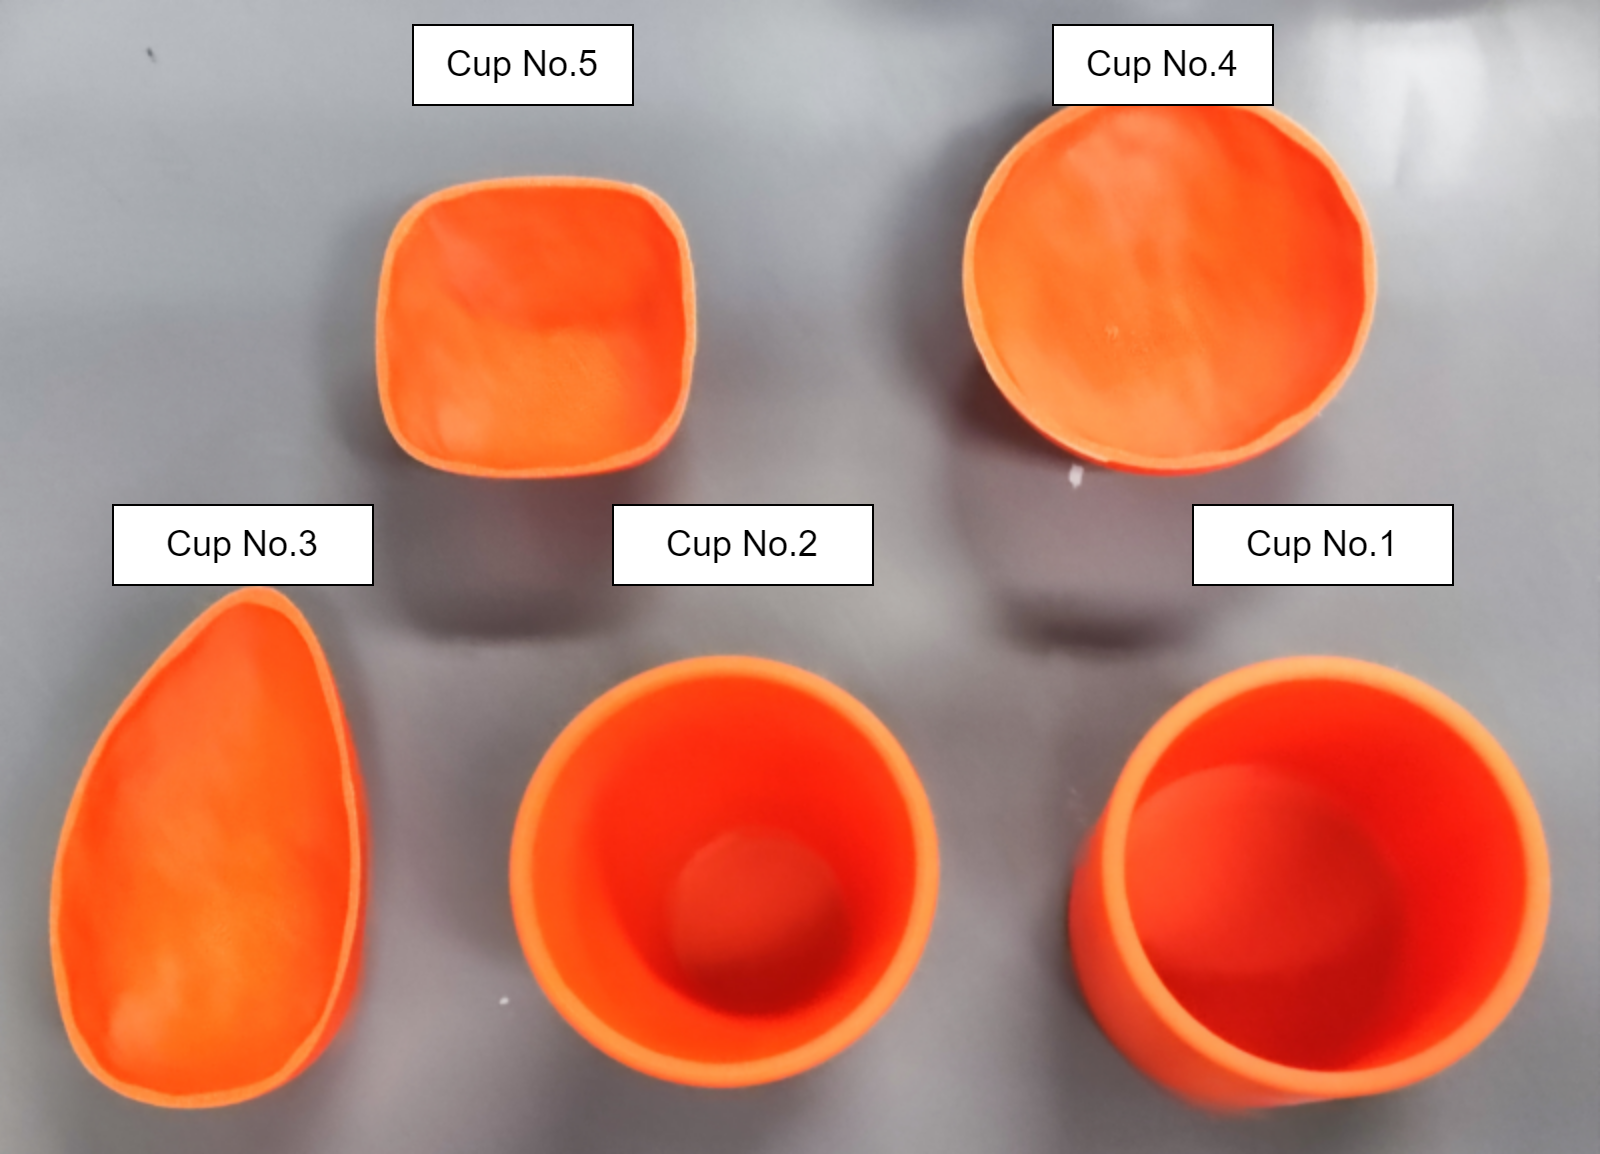
\includegraphics[width=0.7\linewidth]{fig/chp3/chp3_cups.drawio.png}
    \caption{The 3D-Printed cups used in experiment section \ref{sec:system:pointcloud:evaluation:3d-printed-object}.}
    \label{fig:system:pointcloud:evaluation:3d-printed-object}
\end{figure}

次に，標準物体よりも複雑な形状をもつ対象に対して，提案パイプラインがタスクに必要な幾何情報を抽出できるかを評価した．
対象物は，図\ref{fig:system:pointcloud:evaluation:3d-printed-object}で示した，3Dプリンタで作製した5種類の容器であり，それぞれCup 1-5と呼ぶ．
これらは開口部形状，側面曲率，底面形状，および傾斜部の有無が異なるため，容器モデル取得における典型的な形状差を含んでいる．
評価は，容積計算精度と表面形状誤差の二つの観点から行った．

\paragraph{容積計算の評価}

容積の真値は，容器に水を満たし，液面を容器上端と一致させた状態で水の重量を測定し，水の密度を用いて体積へ換算することで得た．
各容器について6回の測定を行い，その平均値を真値$V_{\mathrm{GT}}$とした．
カメラ計測値は，第\ref{sec:system:pointcloud:basic-information}節で述べた$z$方向スライスに基づく断面積分により計算した．
各スライスでは，断面点群を平面に投影し，Convex Hullの面積を断面積として求めた後，隣接スライス間の体積を台形近似で積算した．

表\ref{tab:system:container-volume}に容積計算結果を示す．
表中の設計容積は参考値であり，誤差計算には水重量測定の平均値を真値として用いた．

\begin{table}[t]
  \centering
  \caption{Volume estimation results for 3D-printed containers.}
  \label{tab:system:container-volume}
  \small
  \begin{tabular}{lrrrrr}
    \toprule
    \textbf{Object} & \textbf{Design} & \textbf{GT} & \textbf{Estimated} & \textbf{Error} & \textbf{Rel. err.} \\
     & \textbf{[$\mathrm{cm}^3$]} & \textbf{[$\mathrm{cm}^3$]} & \textbf{[$\mathrm{cm}^3$]} & \textbf{[$\mathrm{cm}^3$]} & \textbf{[\%]} \\
    \midrule
    Cup 1 & 575.48 & $569.92\pm0.97$ & 574.10 &  4.18 & 0.73 \\
    Cup 2   & 366.13 & $362.00\pm0.55$ & 374.48 & 12.48 & 3.45 \\
    Cup 3 & 194.70 & $193.38\pm0.56$ & 184.40 & -8.98 & 4.65 \\
    Cup 4 & 221.05 & $218.92\pm0.39$ & 217.88 & -1.04 & 0.47 \\
    Cup 5 & 140.83 & $141.63\pm0.70$ & 138.45 & -3.18 & 2.25 \\
    \bottomrule
  \end{tabular}
\end{table}

5種類の容器に対する平均絶対誤差は5.97\,$\mathrm{cm}^3$，平均相対誤差は2.31\%であった．
Cup 1およびCup 4では相対誤差が1\%未満であり，提案した点群取得と断面積分により，単純な円筒形状だけでなく曲面を含む容器でも高い精度で容積を推定できることが分かった．
一方，Cup 2では推定値が真値より12.48\,$\mathrm{cm}^3$大きく，Cup 3では8.98\,$\mathrm{cm}^3$小さかった．
この差は，断面積をConvex Hullで近似することによる影響と，容器内部の点群密度の偏りによる影響が大きいと考えられる．
特に，凹部やくびれを含む断面ではConvex Hullが実際の内側形状より広い領域を囲むため，体積が過大評価される可能性がある．
反対に，深い容器や角部を持つ容器では，内壁の一部が視線方向に対して隠れ，断面点群が不足することで断面積が過小評価される場合がある．
Cup 5のように開口部や側面に傾斜を含む容器では，スライスの上端判定と縁付近の点群欠損が体積誤差に影響する．
以上より，本手法は5\%以内の相対誤差で容積を推定できる一方，非凸断面や深い内壁を持つ容器では，Convex Hull近似だけでなく断面輪郭の凹形状を保持する処理を導入することで，さらなる精度向上が期待できる．

\paragraph{表面形状誤差の評価}

同じ5種類の3Dプリンタ製物体について，点群モデルの表面形状再現性を評価した．
真値形状として設計時のCADモデルを用い，取得点群に対してMLS平滑化を適用した後，CADモデルとICPで位置合わせした．
その後，式(\ref{eq:system:point_to_model_distance})に従い，各点からCADモデル表面までの最短距離を計算し，平均値，標準偏差，およびRMSEを求めた．
撮影姿勢は，対象物の周囲$-180^{\circ}$から$+180^{\circ}$まで10$^{\circ}$刻みで設定し，斜め上方から容器内部が見える姿勢を用いた．

表\ref{tab:system:container-surface-error}に表面形状誤差の結果を示す．

\begin{table}[t]
  \centering
  \caption{Surface distance errors between scanned point clouds and CAD models.}
  \label{tab:system:container-surface-error}
  \small
  \begin{tabular}{lrrr}
    \toprule
    \textbf{Object} & \textbf{Avg. [mm]} & \textbf{Std. [mm]} & \textbf{RMSE [mm]} \\
    \midrule
    Cup 1 & 1.952 & 2.931 & 3.522 \\
    Cup 2   & 1.066 & 0.945 & 1.424 \\
    Cup 3 & 1.929 & 1.465 & 2.422 \\
    Cup 4 & 1.482 & 1.201 & 1.907 \\
    Cup 5 & 2.723 & 1.954 & 3.352 \\
    \bottomrule
  \end{tabular}
\end{table}

表面距離誤差の平均値は1.066--2.723\,mm，RMSEは1.424--3.522\,mmであった．
5物体全体の平均RMSEは2.53\,mmであり，取得点群はCADモデルに対して数mm程度の範囲で整合していることが分かる．
最も小さい誤差を示したCup 2では，平均誤差が1.066\,mm，RMSEが1.424\,mmであり，多視点合成とMLS平滑化が有効に働いた．
一方，Cup 1およびCup 5ではRMSEが3\,mmを超えた．
Cup 1の誤差が大きくなった原因としては，容器サイズが大きく，視点間の重複領域における微小な位置合わせ誤差が全体に蓄積したことが考えられる．
また，Cup 5は傾斜面を含むため，視線入射角が大きい領域で深度欠損が発生しやすく，局所的な点群密度低下がRMSEを増加させたと考えられる．

これらの結果は，提案パイプラインが単純な標準物体だけでなく，容器のような自由曲面を含む対象にも適用可能であることを示している．
ただし，CADモデルとの誤差には，RGB-Dカメラの計測誤差だけでなく，3Dプリント時の造形誤差，表面反射，点群平滑化による細部形状の丸め込みも含まれる．
したがって，本結果はカメラ単体の深度精度ではなく，本論文で用いる「撮影--統合--処理--モデル化」全体の実用的な形状再現精度を表すものとして解釈するべきである．

\subsection{底面点群取得の評価}
\label{sec:system:pointcloud:evaluation:bottom-surface}

\paragraph{実験条件}

第\ref{sec:system:bottom_acquisition_flow}節で述べた把持利用型の底面点群取得手法を評価した．
通常の卓上撮影では，対象物と作業台が接触する底面側はカメラから観測できない．
そこで，まず対象物を把持しない状態でサーボハンドの関節角を記録し，次にその関節角を再現してハンドのみの点群を撮影した．
その後，対象物を把持して持ち上げ，$-180^{\circ}$から$+180^{\circ}$まで30$^{\circ}$刻みの視点から底面側を撮影した．
さらに，手指によって遮蔽される領域を減らすため，対象物を一度置き直し，ハンドを$z$軸周りに90$^{\circ}$回転させた状態で同じ手順を繰り返した．
得られた点群からハンドのみの点群を差し引き，式(\ref{eq:system:bottom_restore_point})に基づいてテーブル上の基準姿勢へ復元した後，上面・側面点群と統合した．

\begin{figure}[!t]
    \centering
    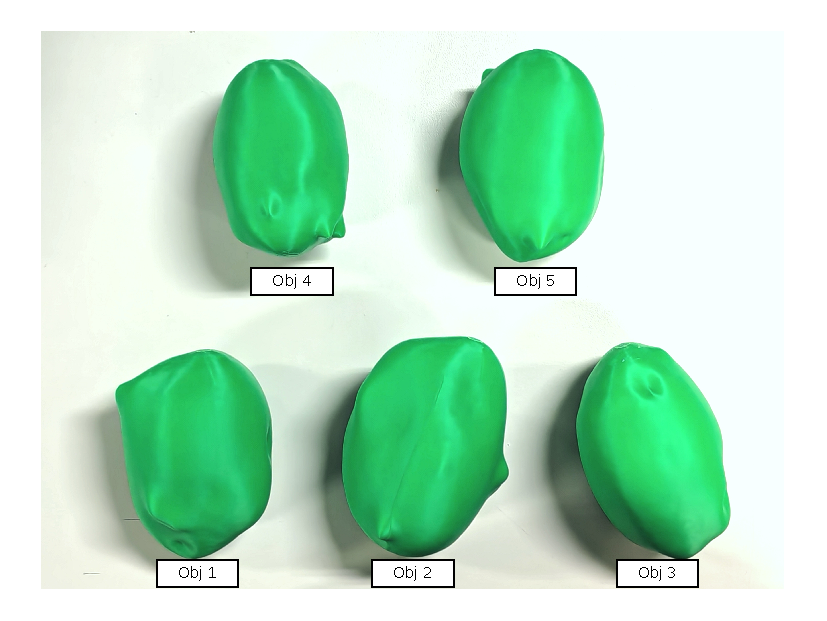
\includegraphics[width=0.8\linewidth]{fig/chp3/chp3_random_potato.drawio.pdf}
    \caption{The 3D-Printed objects used in experiment section \ref{sec:system:pointcloud:evaluation:bottom-surface}.}
    \label{fig:system:pointcloud:evaluation:bottom-surface}
\end{figure}
評価対象は，図\ref{fig:system:pointcloud:evaluation:bottom-surface}に示した，3Dプリンタで作製した5種類の物体である．
真値形状には各物体のCADモデルを用い，ICP位置合わせ後に各点からCADモデルまでの最短距離を計算した．
評価指標は，距離誤差の平均値，標準偏差，およびRMSEである．

\paragraph{結果と考察}

表\ref{tab:system:bottom-pointcloud}に底面点群を含めて取得したモデルの距離誤差を示す．

\begin{table}[t]
  \centering
  \caption{Distance errors of point clouds including bottom-surface acquisition for each object in figure.\ref{fig:system:pointcloud:evaluation:bottom-surface}.}
  \label{tab:system:bottom-pointcloud}
  \small
  \begin{tabular}{lrrr}
    \toprule
    \textbf{Object} & \textbf{Avg. [mm]} & \textbf{Std. [mm]} & \textbf{RMSE [mm]} \\
    \midrule
    Obj 1 & 4.769 & 3.056 & 5.715 \\
    Obj 2 & 4.890 & 3.567 & 6.091 \\
    Obj 3 & 5.095 & 4.446 & 6.768 \\
    Obj 4 & 5.238 & 3.419 & 6.327 \\
    Obj 5 & 4.910 & 4.673 & 6.789 \\
    \bottomrule
  \end{tabular}
\end{table}

5物体の平均距離誤差は4.98\,mm，平均RMSEは6.34\,mmであった．
物体間で平均誤差の差は小さく，最小値はObj 1の4.769\,mm，最大値はObj 4の5.238\,mmであった．
このことから，提案した底面点群取得手順は，対象形状が異なっても同程度の精度で底面側を補完できることが分かる．
一方，表面形状誤差の評価（表\ref{tab:system:container-surface-error}）と比較すると，底面点群を含む場合のRMSEは大きい．
この増加には，持ち上げ時の把持による対象物姿勢の微小変化，ハンド点群除去時の残留点，手指遮蔽による局所的欠損，および持ち上げ姿勢からテーブル上姿勢へ復元する際のロボット手先姿勢誤差が影響していると考えられる．

それでも，底面点群を取得する意義は大きい．
卓上撮影だけでは，底面側は完全に欠落し，点群モデルは上面および側面に偏った開いた形状となる．
これに対して，本手法では把持・持ち上げ・再撮影を用いることで，底面および下部側面を含む閉じた外形に近い点群を得ることができる．
この情報は，物体の幾何学的重心の近似，把持候補点の生成，および安定把持における接触可能領域の評価に有効である．
したがって，底面取得では局所的な誤差は増加するものの，対象物全体の幾何情報を補完するという目的に対しては有効であると考えられる．

\subsection{本セクションのまとめ}

以上の三種類の評価実験から，提案した3D点群モデル取得パイプラインは，標準物体に対しては半径1\,mm未満，位置1--2\,mm程度の誤差で幾何プリミティブを推定できることが確認された．
また，3Dプリンタ製容器に対しては，平均相対誤差2.31\%で容積を推定でき，CADモデルに対する表面RMSEは1.424--3.522\,mmであった．
底面点群取得では，RMSEが5.715--6.789\,mmと大きくなるものの，卓上撮影では取得できない底面側の幾何情報を補完できることを確認した．
これらの結果は，本章で構築した点群取得・処理パイプラインが，後続章の皮むき，注ぎ，および安定把持に必要な幾何情報を提供できることを示している．

\section{まとめ}
\label{sec:system:summary}

本章では，本論文におけるロボットシステムの構成と3D点群モデル取得の共通処理パイプラインについて述べた．
本章の主要な内容を以下に要約する：

\begin{enumerate}
  \item \textbf{ロボットシステムの構成}：双腕ロボット（PA10-7C / DENSO VS-050），力覚センサ，平行グリッパ，RGB-Dカメラからなるハードウェア基盤を構築した．また，三つのタスクそれぞれに適切なエンドエフェクタを設計・実装した．

  \item \textbf{点群取得}：RGB-Dカメラを用いた多視点点群撮影，座標系定義（世界・カメラ・手先の3階層），Hand-Eyeキャリブレーションによる外部パラメータ同定，座標変換による多視点点群合成の手順を確立した．これにより，単一視点では不可視となる領域を含む全周的な物体形状の取得が可能となった．

  \item \textbf{点群処理}：作業領域切り出し，Voxel Gridダウンサンプリング，RANSACによる平面除去，Statistical/Radius Outlier Removalによる外れ値除去，Euclidean Clusteringによる対象物抽出，MLS平滑化と法線ベクトル推定からなる標準処理パイプラインを構築した．これにより，ノイズや作業台平面を除外した高品質な物体点群モデルが得られることを確認した．

  \item \textbf{基礎情報の抽出}：前処理後の点群モデルから，位置姿勢（AABB），色情報，法線ベクトル，断面積と体積（Quickhull凸包＋断面積分），重心，表面領域と指先位置候補を抽出する手法を示した．これらの情報は，後続章における液体注ぎ制御，食材把持位置探索，皮むき軌道生成の基盤となる．

  \item \textbf{底面点群の取得}：机上スキャンで不可視となる底面情報を，把持による持ち上げと再撮影により取得する手法を提案した．さらに，手指遮蔽を低減するためにハンドを$z$軸周りに90$^{\circ}$回転させて再撮影する手順を導入し，底面を含む外形点群を構成できることを確認した．

  \item \textbf{精度評価}：標準物体，3Dプリンタ製容器，および底面点群取得の評価実験により，点群取得・処理パイプラインの実用的な精度を確認した．円柱標準物体では半径誤差が全条件平均で$-0.716\pm0.175$\,mmであり，3Dプリンタ製容器では容積推定の平均相対誤差が2.31\%，CADモデルに対する表面RMSEが1.424--3.522\,mmであった．底面点群を含むモデルではRMSEが5.715--6.789\,mmとなり，底面補完に伴う誤差増加と全体形状補完の効果を確認した．
\end{enumerate}

\begin{revisionblock}
以上の結果から，本章で構築したロボットシステムと点群取得・処理パイプラインは，後続章の三タスクについて必要な幾何情報を供給できることを確認した．
ただし，RGB-D計測には反射・透明表面や遮蔽による欠測があり，底面を含むモデルでは誤差も増加するため，本結果から物体操作一般に対する十分な精度または汎用性を主張するものではない．
家庭用システムへの展開には，装置の小型化，計測時間の短縮，およびキッチンに存在する反射・透明物体に対する追加のロバスト化が必要である．
\end{revisionblock}

	\chapter{タスク1：皮むき作業}
\label{ch:peeling}

本章では，第\ref{ch:introduction}章で設定した第一の研究課題である皮むき動作を扱う．
第\ref{ch:system}章で構築した3D点群モデル取得の共通基盤の上に，食材の皮むき動作を実現するための具体的なアルゴリズムと制御手法を述べる．
皮むき動作は，第1章で述べた「分析主導型」アプローチにおける「幾何学的な分析」の代表的な適用例であり，3D点群モデルから抽出した表面の法線や曲率といった幾何特徴に基づいて動作軌道を生成し，実行時には力覚フィードバックにより接触状態を維持するという，幾何と力学の統合が求められるタスクである．

本章で扱う皮むき動作は，一方のロボットアームがピーラーを把持し，他方のロボットアームが食材を支える双腕共同作業として構成される．
対象とする食材の表面形状には個体差が大きく，事前のCADモデルが利用できないため，その場で取得した3D点群モデルから動作計画に必要な幾何情報を抽出することが必須となる．
また，ピーラーの刃先を食材表面に沿って移動させる際には，単なる位置制御では点群計測誤差や表面の凹凸に対応できないため，力覚フィードバックによる接触力の維持が不可欠である．

以下では，まず皮むき動作の問題設定と全体手順を整理し，続いて幾何情報に基づく軌跡生成・分割・回転角計算の手法を述べ，さらにそれらを用いた動作計画と力覚フィードバック制御の統合について論じる．
最後に，複数種類の食材を用いた実機実験により，提案手法の有効性を検証する．

% 数字番号は，章・節タイトルではなく，上位節の中で説明する処理手順を表す．
% 本章では，第3章で得られた食材表面の3D点群モデルを入力とし，
% 点群取得，座標変換，多視点統合，平滑化，法線推定などの共通処理は繰り返して述べない．
% 符号は一括して冒頭に列挙せず，各処理の説明の中で必要に応じて定義する．

\section{皮むき動作の概要}  %% TODO整体的构成不太好
\label{sec:peeling_phase_overview}

本節では，本章で扱う皮むき動作の問題設定，作業全体の流れ，および使用する点群情報を整理する．
ここでは，アルゴリズムの詳細には入らず，本章全体の見取り図を与える．

\subsection{問題設定}
{
% TODO: 这两段说如何简化这个课题，真的可以么;这部分内容 感觉不像问题设定
皮むき動作では，一方のロボットアームがピーラーを把持し，他方のロボットアームが食材を支える双腕構成をとる．
本研究では調理器具として包丁ではなくピーラーを採用する．この選択には以下の二つの理由がある．

第一に，ピーラーの刃には切り込み深さを制限するリミッター（刃の間隔が固定する構造）が備わっている．
このリミッターにより，ピーラーを食材表面に一定の力で接触させ，目的の皮むき方向へ移動させるだけで，適切な深さの皮むきが実現される．
すなわち，包丁のように刃の角度や押し込み量を精密に制御する必要がなく，接触力の維持のみで皮むき動作が成立する．

第二に，ピーラーを用いることで，皮むき作業が「ピーラーを動かして一部の皮を剥く操作」と「食材を回転させて皮むき位置を変える操作」の二つに明確に分離される．
包丁では両手の協調動作が常時必要となるが，ピーラーではピーラー側の腕と食材固定側の腕の役割が時間的に独立するため，各操作の計画と制御が容易になる．

このような理由から，本タスクではピーラーを用い，対象とする食材の表面形状を $S$ とし，食材は串に固定されて回転軸 $\mathbf{v}_{\mathrm{rot}}$ 周りに回転できるものとする．
ピーラー側の腕は，食材表面に沿って刃先を移動させることで一部の皮を剥く「一回皮むき動作」を実行する．
食材固定側の腕は，一回皮むき動作が終了した後，未処理領域がピーラー側に来るように食材を回転させる「食材の回転操作」を実行する．
}

本章で解く問題は，以下のように整理できる．

\begin{enumerate}
  \item 食材表面の3D点群モデルから，ピーラーが倣うべき基準軌跡を生成する．
  \item 食材表面の法線変化に基づき，基準軌跡を実行しやすい複数の軌跡区間へ分割する．
  \item ピーラーと食材表面の接触を維持するため，力覚フィードバックを用いて刃先位置を補正する．
  \item 非皮領域の境界を検出し，次回の食材回転角を決定する．
  \item 皮むき動作と食材回転を反復し，終了条件を満たすまで皮むき範囲を拡大する．
\end{enumerate}

この問題設定は，人間がピーラーを用いて食材表面を一方向に剥き，その後食材を回して隣接領域を剥く手順を，双腕ロボット上で実現することに相当する．
人間は，食材の形状を視覚で捉えながらピーラーの刃先を表面に沿って滑らせ，適宜食材を回転させて未処理領域へと作業範囲を拡大していく．
本研究では，これらの機能を3D点群モデルに基づく幾何解析と力覚フィードバック制御の組み合わせにより工学的に実現する．

本タスクでは，以下の三つの仮定を置く．

\begin{enumerate}
  \item 対象食材は一つの代表的な中心軸を有し，その軸を基準として回転操作が可能であるものとする．この中心軸を食材の回転軸 $\mathbf{v}_{\mathrm{rot}}$ とし，皮むき軌跡の生成および皮むき後の食材回転に用いる．
  \item 食材は作業台 $\mathcal{P}_T$ 上に置かれており，作業台平面の法線ベクトル $\mathbf{n}_{\mathrm{ct}}$ は世界座標系の $z$ 軸方向と常に一致する．
  \item 一回皮むき動作で剥かれる領域は，幅が一定の矩形形状となる．すなわち，剥かれた皮の幅は軌跡上の全位置で同一である．
\end{enumerate}

これらの仮定のもとで，提案手法は食材の個体差（形状，大きさ，表面曲率）に対して適応的に皮むき動作を生成することを目指す．

\subsection{皮むき動作の全体手順}

皮むき作業は，「一回皮むき動作」と「食材の回転操作」の反復として構成する．
ここで，一回皮むき動作とは，ピーラーを食材表面に接触させ，あらかじめ生成した軌跡に沿って移動させる処理である．
食材の回転操作とは，一回皮むき動作の後に，次に剥くべき領域がピーラー側へ向くように食材を回転させる処理である．

全体手順は以下のように整理できる（図\ref{fig:peeling_sequence}）．

\begin{enumerate}
  \item 第3章の手順により得られた食材表面のRGB点群 $P_{\mathrm{all}}$ を入力する．
  \item 食材の回転軸 $\mathbf{v}_{\mathrm{rot}}$ を含む断面抽出平面を用いて，食材断面を抽出する．
  \item 断面輪郭から，到達困難な下側部分を除去し，到達可能な基準軌跡 $L$ を得る．
  \item 基準軌跡 $L$ 上の法線変化を用いて，軌跡を複数のセグメント $s_j$ に分割する．
  \item 各セグメントに沿ってピーラーを移動させ，力覚フィードバックにより接触力を維持する（一回皮むき動作の実行）．
  \item 一回皮むき動作の後，RGB情報を用いて非皮領域とその境界 $L_p$ を抽出する．
  \item 境界近傍の平均法線 $\mathbf{n}_{\mathrm{avg}}$ から，食材の回転角 $\alpha$ を計算する．
  \item 食材を $\mathbf{v}_{\mathrm{rot}}$ 周りに $\alpha$ だけ回転させ，次の一回皮むき動作へ移る．
  \item 終了判定を満たすまで，必要に応じて点群を再取得しながら，ステップ2〜8を反復する．
\end{enumerate}

% TODO：图的位置不对
% \begin{figure}[t]
%     \centering
%     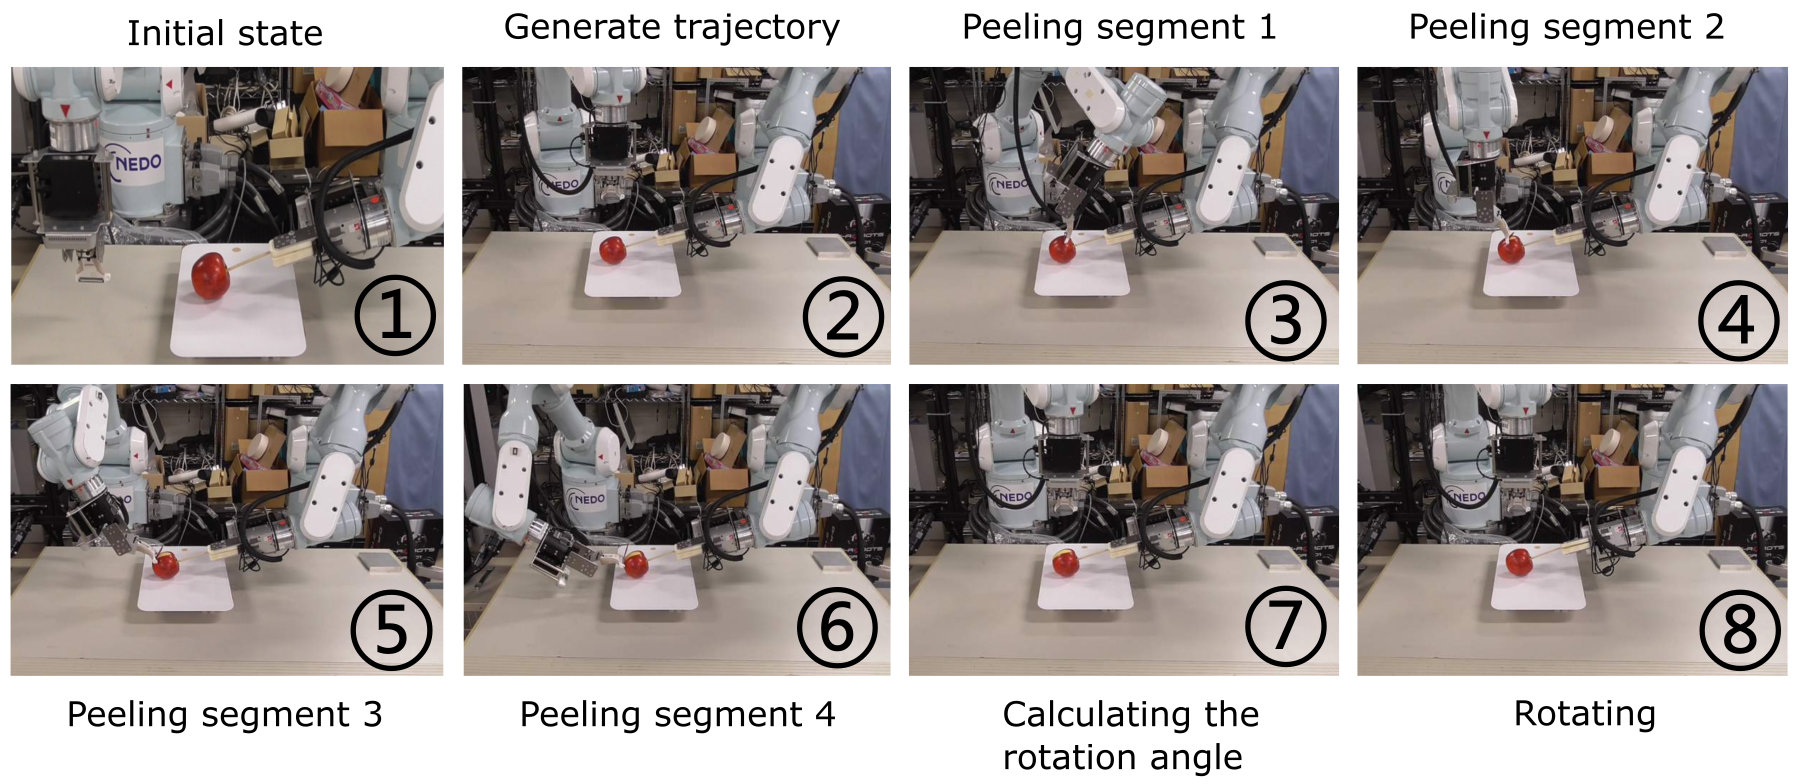
\includegraphics[width=0.7\textwidth]{fig/chp_peeling/sequence.png}
%     \caption{提案する皮むき手法の全体シーケンス．終了条件を満たさなければ，Step~8 の後 Step~2 へ戻る．}
%     \label{fig:ch4_sequence}
% \end{figure}

ここでは，$P_{\mathrm{all}}$，$L$，$s_j$，$L_p$，$\alpha$ などの符号を，全体手順の中で必要な順に導入する．
以降の節では，これらの量をどのように求め，ロボットの動作へ接続するかを述べる．

\subsection{使用する点群情報}

本章で使用する点群情報は，第3章で述べた3Dモデル取得手順により得られたものである．
具体的には，以下の情報を用いる．

\begin{enumerate}
  \item \textbf{食材表面点群 $P_{\mathrm{all}}$} \\
  食材全体の外表面を表すRGB点群であり，基準軌跡の抽出，非皮領域の検出，終了判定に用いる．
  $P_{\mathrm{all}}$ は，第3章の共通処理パイプライン（多視点撮影，座標変換，統合，ダウンサンプリング，外れ値除去，クラスタリング，MLS平滑化）を経て得られたものであり，各点は3次元座標 $(x, y, z)$，RGB色情報，および法線ベクトル $\mathbf{n}_i$ を有する．
  法線ベクトルはMLS（Moving Least Squares）法\cite{PCL-MLS}により計算され，食材の外側を向くよう統一されている．

  \item \textbf{表面点 $\mathbf{p}_i$ と法線 $\mathbf{n}_i$} \\
  点群中の各点を $\mathbf{p}_i$，その法線を $\mathbf{n}_i$ とする．
  法線情報は，軌跡分割，ピーラー姿勢の決定，食材回転角の計算に用いる．

  \item \textbf{RGB情報} \\
  皮と非皮領域の色差を利用し，非皮領域および境界 $L_p$ を抽出するために用いる．
  具体的には，RGB色空間からHSV色空間への変換を行い，事前に定義されたHSV範囲に基づいて非皮領域を識別する．

  \item \textbf{作業台平面と回転軸} \\
  作業台平面を $\mathcal{P}_T$，その法線を $\mathbf{n}_{\mathrm{ct}}$ とする．
  作業台平面の法線 $\mathbf{n}_{\mathrm{ct}}$ は，第3章で述べたRANSAC法\cite{PCL-RANSAC}により点群から自動抽出される．
  また，食材の回転軸を $\mathbf{v}_{\mathrm{rot}}$ とする．これは食材の中心軸として人手により指定される．
  これらは，断面抽出と食材回転を記述する基準として用いる．
\end{enumerate}

これらの点群情報は，いずれも第3章の共通処理パイプラインを経て取得されるため，本章では個々の取得手順を繰り返し述べることはせず，必要に応じて第3章の該当節を参照する形で記述を進める．

\section{幾何情報による皮むき動作の分析}
\label{sec:peeling_phase_geo}

本節では，食材表面の3D点群モデルから，皮むき動作に必要な幾何情報を抽出する方法を述べる．
具体的には，断面輪郭に基づく基準軌跡の抽出，表面法線による軌跡分割，および非皮領域境界に基づく回転角の計算を扱う．
これらの処理は，本論文の「分析主導型」アプローチにおける「幾何学的な分析」の中核をなすものであり，物理的な接触を伴わない事前の計算段階で，食材形状に適応した動作パラメータを導出することを目的とする．

\subsection{軌跡の抽出}
\label{sec:peeling_trajectory}

一回皮むき動作では，ピーラーの刃先が食材表面に沿って移動する必要がある．
食材の形状は個体ごとに異なるため，あらかじめ固定された軌跡を用いることはできず，その場で取得した食材表面点群から基準軌跡を抽出する必要がある．
仮定より，食材は回転軸 $\mathbf{v}_{\mathrm{rot}}$ 周りのみに回転するため，各回の皮むきで最大の剥き幅を得るには，刃先を表面に沿って，かつ回転軸 $\mathbf{v}_{\mathrm{rot}}$ に「平行」に滑らせるのが最も単純かつ効果的な方法である．

そこで，以下の手順により基準軌跡を生成する．

\subsubsection{断面抽出平面1による断面輪郭の抽出}

まず，食材の回転軸 $\mathbf{v}_{\mathrm{rot}}$ を含み，作業台平面 $\mathcal{P}_T$ に垂直な平面を断面抽出平面 $\mathcal{P}_{c1}$ として定義する．
$\mathcal{P}_{c1}$ は，食材の回転軸に沿った鉛直断面を切り出すための平面である．

この断面抽出平面 $\mathcal{P}_{c1}$ により食材形状 $\mathrm{S}$ を切断し，断面領域 $A_c$ と断面輪郭 $L_c$ を得る．
実際の処理では，食材表面点群 $P_{\mathrm{all}}$ から $\mathcal{P}_{c1}$ に近い点（点と平面の距離が閾値以内の点）を抽出し，それらを断面輪郭 $L_c$ の離散表現とする．
今回の実験では，この閾値を0.3\,mmとした．この値は，使用する点群の密度に依存して定められる．

\subsubsection{到達可能軌跡の抽出}

断面輪郭 $L_c$ の全体がロボットにとって実行可能な軌跡になるわけではない．
食材の下側部分，すなわち作業台に近い領域は，作業台やロボットアーム，串固定部との干渉により到達が困難である．
そのため，到達可能性を判定するための到達可能性判定平面2 $\mathcal{P}_{c2}$ を導入し，$L_c$ のうち到達困難な部分を除去する．

$\mathcal{P}_{c2}$ は，回転軸 $\mathbf{v}_{\mathrm{rot}}$ を通り，その法線 $\mathbf{n}_{c2}$ が以下の条件を満たす平面として定義される．

\begin{align}
  \mathbf{n}_{c2} &= \mathbf{r} \times \mathbf{n}_p \label{eq:peeling_cut_plane_2}
\end{align}

ここで，$\mathbf{n}_p$ は以下の条件を満たすベクトルである．

\begin{equation}
  \mathbf{n}_p \cdot \mathbf{n}_{\mathrm{ct}} = 0,\quad
  \mathbf{n}_p \cdot \mathbf{v}_{\mathrm{rot}} = 0,\quad
  \mathbf{n}_p \cdot \mathbf{n}_{\mathrm{ct}} \ge 0
\end{equation}

すなわち，$\mathbf{n}_p$ は $\mathcal{P}_{c2}$ 上にあり，回転軸 $\mathbf{v}_{\mathrm{rot}}$ と作業台平面の法線 $\mathbf{n}_{\mathrm{ct}}$ の両方に直交するベクトルである．

断面輪郭 $L_c$ の各点 $\mathbf{p}_i$ に対して，以下の条件を満たす点を到達困難点として除去する．

\begin{equation}
  \mathbf{v}_i \cdot \mathbf{n}_{c2} > 0
  \label{eq:peeling_point_removal}
\end{equation}

ここで，$\mathbf{v}_i$ は世界座標系の原点から点群 $P_{\mathrm{all}}$ 中の点 $\mathbf{p}_i$ へ向かうベクトルである．
除去後に残った輪郭を，到達可能な基準軌跡 $L$ とする．
基準軌跡 $L$ の点群を $P_L$ と表記する．
この処理を図\ref{fig:peeling_trajectory}に示す．

\begin{figure}[t]
    \centering
    \begin{subfigure}[t]{.45\textwidth}
    	\centering
    	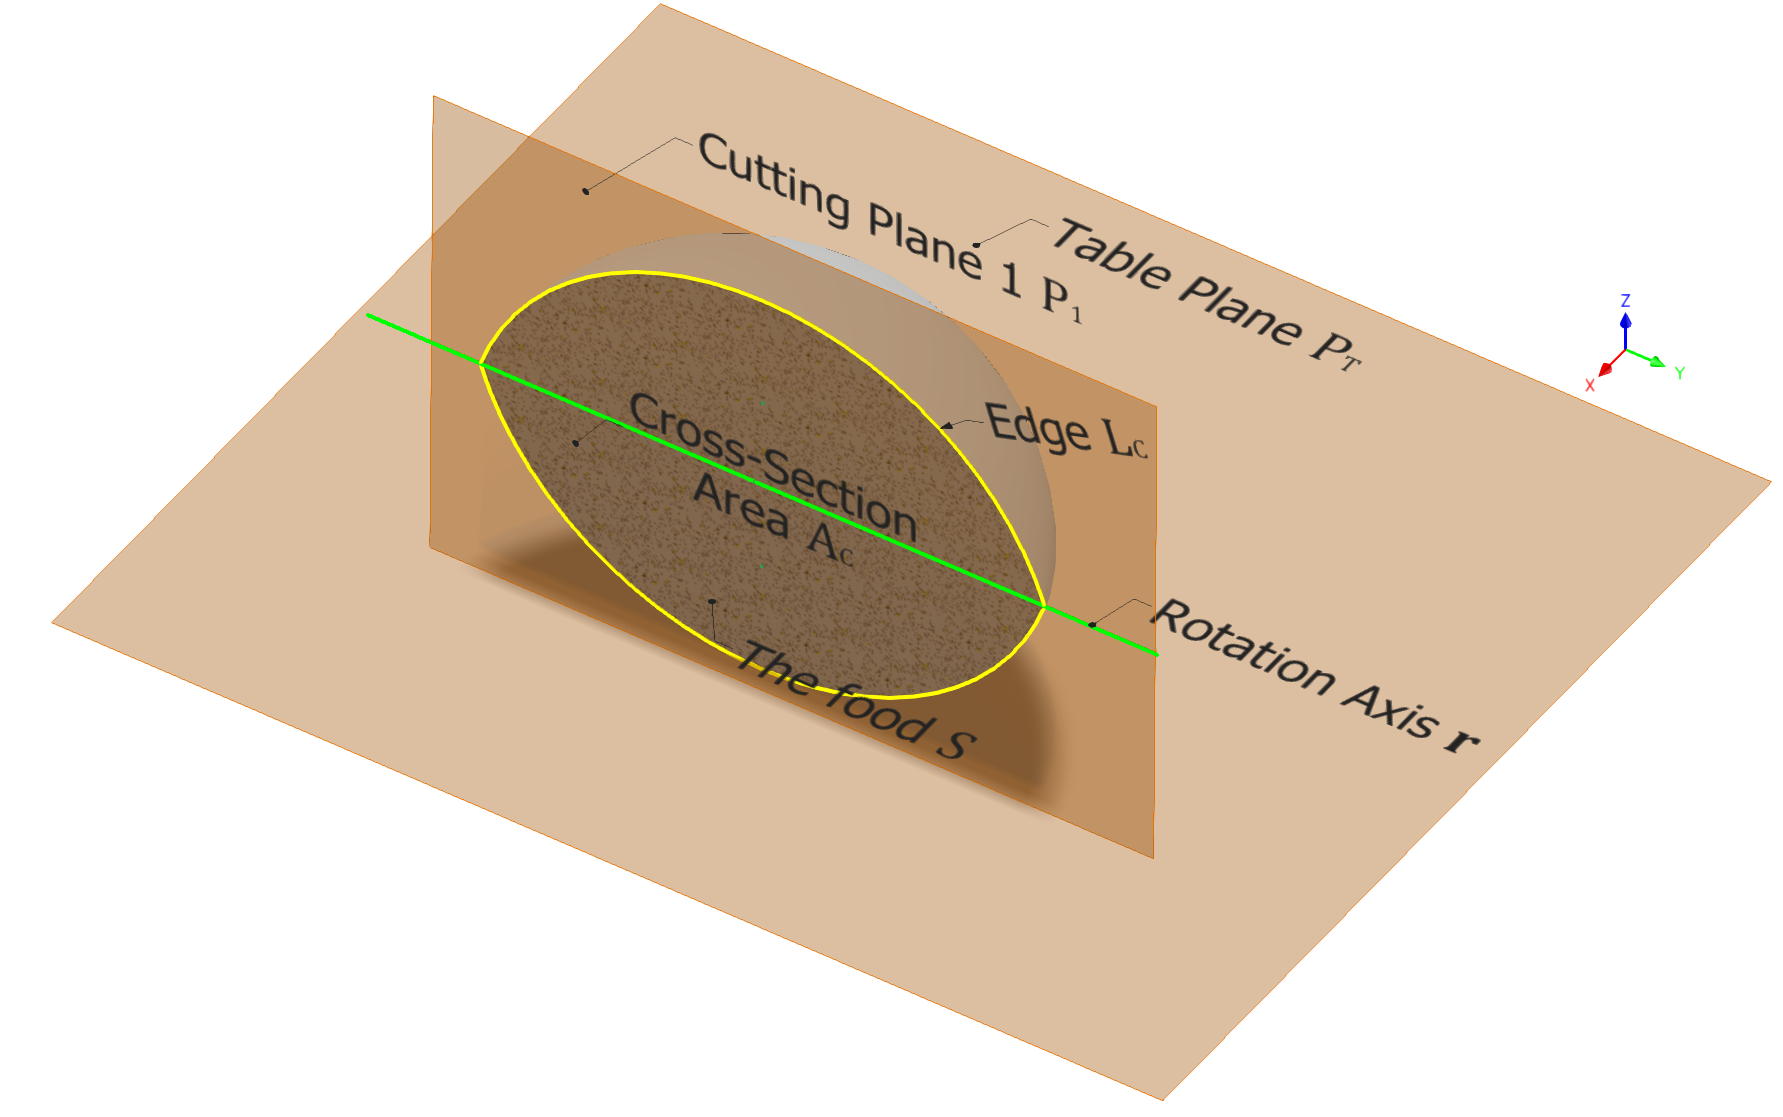
\includegraphics[width=1\textwidth]{fig/chp_peeling/Trajectory_cutting.png}
    	\caption{The cross-section area $\mathrm{A_c}$ that is cut by the cutting plane 1 $\mathcal{P}_\mathrm{c1}$. The yellow line $L_\mathrm{c}$ is the edge of the cross-section area.}
    	\label{fig:peeling_trajectory.sub1}
    \end{subfigure}
    \begin{subfigure}[t]{.45\textwidth}
    	\centering
    	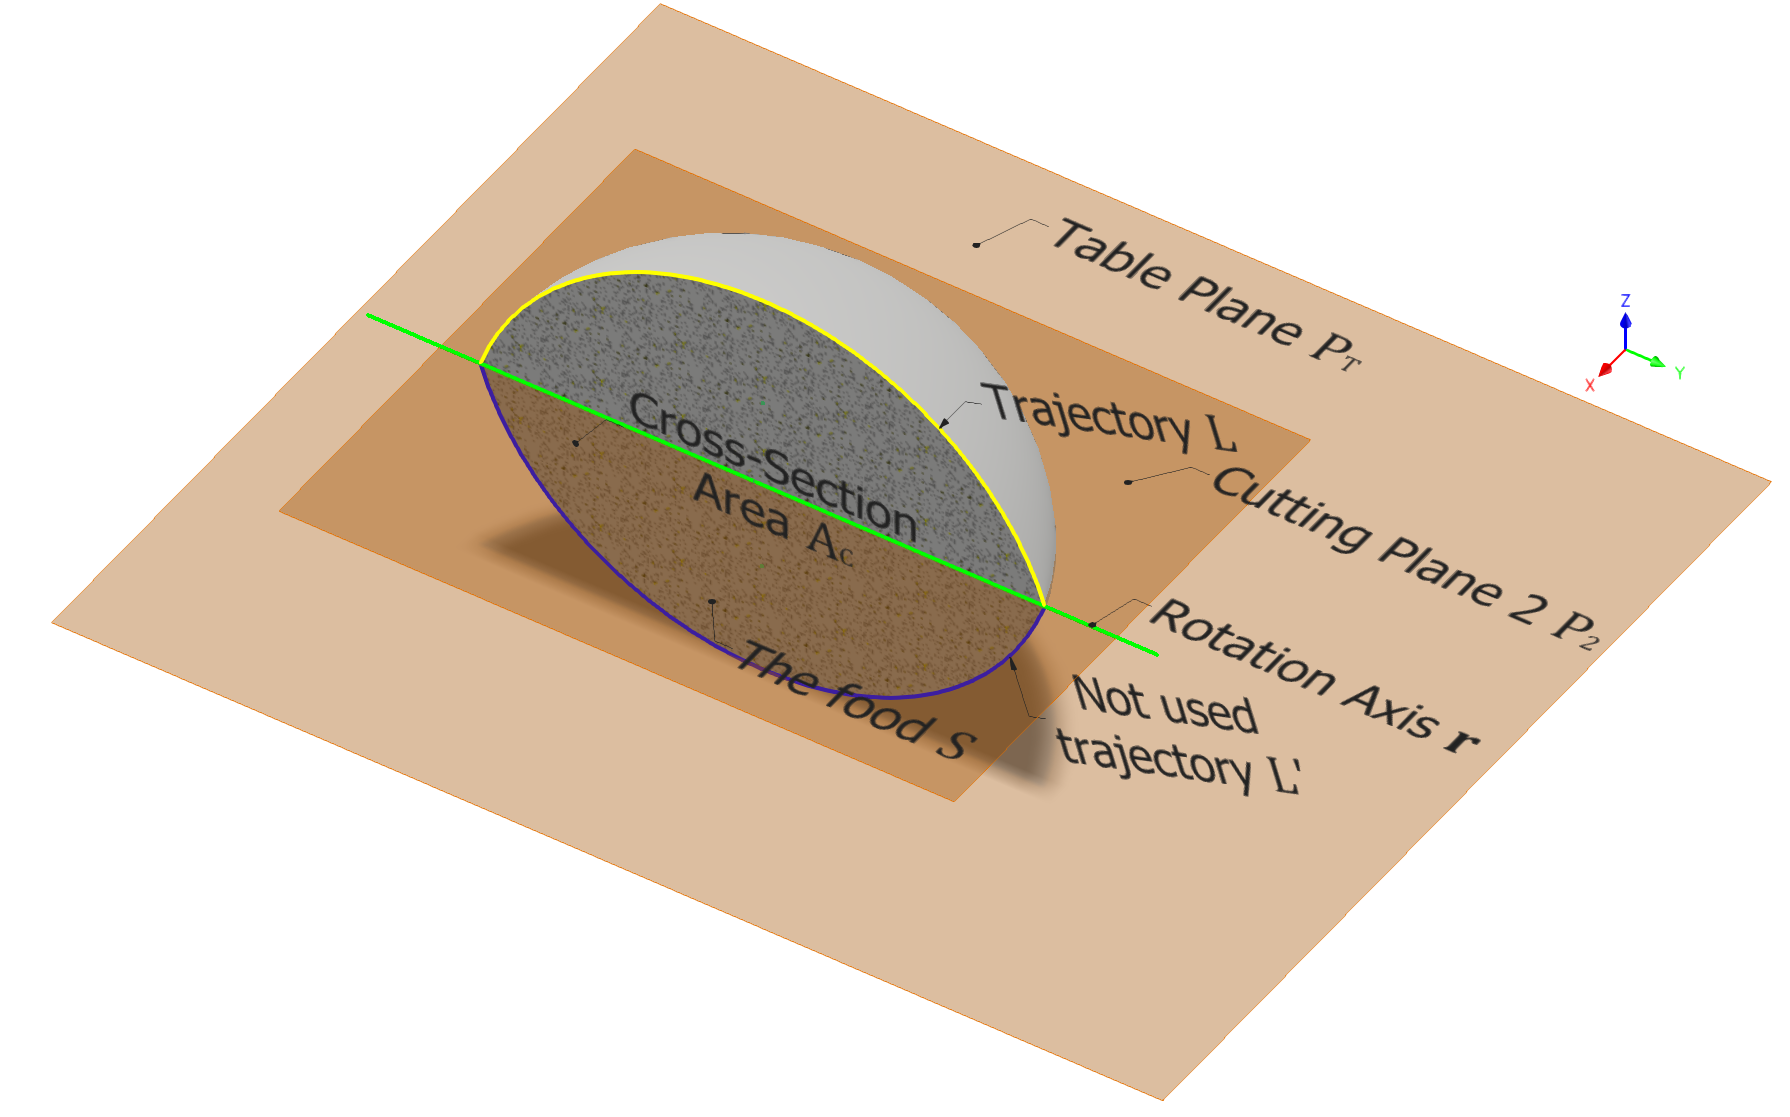
\includegraphics[width=1\textwidth]{fig/chp_peeling/Trajectory.png}
    	\caption{The result of creating the reference trajectory. The yellow line is the final trajectory $L$. The blue line $L'$ (bottom side of the food) is the trajectory that is not used.}
    	\label{fig:peeling_trajectory.sub2}
    \end{subfigure}
    \caption{The gray object is the shape of the food $\mathrm{S}$, which we is subject to peel. The largest plane with orange color is the table plane $\mathcal{P}_T$. The small plane on the left side of the images with orange color, perpendicular to the table plane, is the cutting plane 1 $\mathcal{P}_\mathrm{c1}$. The small plane on the right side of the images with orange color, parallel to the table plane, is the cutting plane 2 $\mathcal{P}_\mathrm{c2}$. The green line is the rotation axis $\mathbf{v_\mathrm{rot}}$ that is determined by human}
    \label{fig:peeling_trajectory}
\end{figure}


以上の処理をまとめると，軌跡抽出の手順は以下の通りである．

\begin{enumerate}
  \item $\mathcal{P}_{c1}$ を，$\mathbf{v}_{\mathrm{rot}}$ を含み，$\mathcal{P}_T$ に垂直な平面として定義する．
  \item $P_{\mathrm{all}}$ から，$\mathcal{P}_{c1}$ への距離が閾値0.3\,mm以内の点を抽出し，断面輪郭 $L_c$ とする．
  \item 式(\ref{eq:peeling_cut_plane_2})により $\mathcal{P}_{c2}$ の法線 $\mathbf{n}_{c2}$ を決定する．
  \item 式(\ref{eq:peeling_point_removal})により $L_c$ から下側部分を除去し，到達可能軌跡 $L$（点群 $P_L$）を得る．
\end{enumerate}

このようにして得られた基準軌跡 $L$ は，食材の回転軸を含む断面輪郭のうち，ロボットアームがピーラーを安全に到達させられる上半分の曲線となる．
本節では基準軌跡 $L$ の生成に焦点を当て，点群の取得，合成，平滑化，および法線推定の詳細は第3章で扱っているため，ここでは繰り返さない．

\subsection{法線による軌跡分割}
\label{sec:peeling_trajectory_segmentation}

抽出された基準軌跡 $L$ は，食材表面の曲率に従う3次元曲線である．
一方，ピーラーの刃は食材表面に対して受動的に回転できる構造を有しているため，ピーラーの持ち手（ハンドル）の姿勢によらず，刃先は自動的に表面に接する方向をとることができる．
この性質により，曲線全体の厳密な追跡は不要であり，軌跡を複数の直線セグメントに分割して逐次実行することが可能となる．
なお，実行時には力覚フィードバックが併用されるため，実際のロボットの移動経路は厳密な直線にはならない．

$P_L$ 上の点を実行順に $\mathbf{p}_1, \mathbf{p}_2, \ldots, \mathbf{p}_N$，対応する法線を $\mathbf{n}_1, \mathbf{n}_2, \ldots, \mathbf{n}_N$ とする．
ここで，点群の実行順への並べ替えは以下のように行う．
まず，$P_L$ の中で $z$ 座標が最大となる点を基準点とする．
基準点よりも右側の点群は，$z$ 座標が最小の点を始点として $z$ 座標の小さい順に並べる．
左側の点群は，基準点を始点として $z$ 座標の大きい順に並べる．
最後に，左右の点列を結合することで，軌跡に沿った順序の点列を得る．

軌跡分割の処理は，以下の手順で行う．

まず，軌跡 $L$ の先端の点 $\mathbf{p}_1$ を現在のセグメントの開始点 $\mathbf{p}_{\mathrm{st}}$ とし，その法線 $\mathbf{n}_1$ を参照法線 $\mathbf{n}_{\mathrm{ref}}$ とする．
次に，点の順番に走査し，各点 $\mathbf{p}_n$ の法線 $\mathbf{n}_n$ と $\mathbf{n}_{\mathrm{ref}}$ のなす角$\theta_n$を計算する．

% \[
% \theta_n = \arccos\left(\frac{\mathbf{n}_n \cdot \mathbf{n}_{\mathrm{ref}}}{\|\mathbf{n}_n\| \cdot \|\mathbf{n}_{\mathrm{ref}}\|}\right)
% \]

このなす角の角度 $\theta_n$ が閾値 $\theta_{\mathrm{th}}$ を超えた場合，$\mathbf{p}_{\mathrm{st}}$ から $\mathbf{p}_{n-1}$ までを一つのセグメント $s_j$ とする．
そして，$\mathbf{p}_n$ を新しいセグメントの開始点 $\mathbf{p}_{\mathrm{st}}$ に設定し，同様の処理を軌跡の終端まで反復する．

今回の実験では，$\theta_{\mathrm{th}} = 30^\circ$ を閾値として用いた．
各セグメント $s_j$ に対して，セグメント内の全点の法線ベクトルを平均したものを $\mathbf{a}_j$ とし，これを当該セグメントにおけるピーラー姿勢の参照方向とする．

処理手順は以下の通りである．

\begin{enumerate}
  \item 基準軌跡 $L$ 上の点群 $P_L$ を実行順に並べる．
  \item 先端の点 $\mathbf{p}_1$ をセグメント開始点 $\mathbf{p}_{\mathrm{st}}$，その法線を $\mathbf{n}_{\mathrm{ref}}$ とする．
  \item 点列に沿って各点 $\mathbf{p}_n$ の法線 $\mathbf{n}_n$ と $\mathbf{n}_{\mathrm{ref}}$ の角度差 $\theta_n$ を計算する．
  \item $\theta_n > \theta_{\mathrm{th}}$ を満たした場合，$\mathbf{p}_{\mathrm{st}}$ から $\mathbf{p}_{n-1}$ までを一つのセグメント $s_j$ とする．
  \item $\mathbf{p}_n$ を新たな $\mathbf{p}_{\mathrm{st}}$ とし，ステップ3〜4を軌跡終端まで反復する．
  \item 得られた各セグメント $s_j$ の平均法線 $\mathbf{a}_j$ をピーラー姿勢決定に用いる．
\end{enumerate}

この軌跡分割により，曲率の大きな食材（例：りんご）では多くのセグメントに分割され，曲率の小さな食材（例：きゅうり，なす）では少数のセグメントとなる．
この適応的な分割が，食材形状の多様性に対する本手法の幾何学的適応能力の一端を担っている．

\subsection{非皮領域境界に基づく回転角の計算}
\label{sec:peeling_rotation_calc}

一回皮むき動作の後，次に剥くべき領域をピーラー側へ向けるためには，食材を適切な角度だけ回転させる必要がある．
仮定より，回転操作は固定された回転軸 $\mathbf{v}_{\mathrm{rot}}$ 周りのみに行われるが，その回転角は皮むきの度に適切に決定されなければならない．
回転角が大きすぎると剥き残しが生じ，小さすぎると既剥き領域を重複して剥くことになり作業効率が低下する．
そこで，一回皮むき動作で実際に非皮領域の境界を検出し，その幾何情報から次回の回転角を計算する手法をとる．

\subsubsection{非皮領域の抽出}

一回皮むき動作の後，ピーラー側の腕を食材の上方へ移動させ，RGB-Dカメラにより食材上面のRGB点群（以下，元RGB点群と呼ぶ）を取得する．
この元RGB点群から，第3章で述べた共通処理を適用し，食材表面のRGB点群 $P_{\mathrm{all}}$ を得る．
さらに，各点の法線ベクトルを計算する．

次に，$P_{\mathrm{all}}$ の各点の色情報をRGB色空間からHSV色空間に変換し，事前に定義された非皮領域のHSV範囲に基づいて，非皮領域の点群を抽出する．
この色範囲は人間が事前に指定する．
抽出された非皮領域点群に対してクラスタリングを適用し，最大クラスタを非皮領域 $P_{\mathrm{cluster}}$ とする．
各食材の非皮領域抽出に用いるHSV範囲の例を表\ref{tab:peeling_hsv_range}に示す．

\begin{table}[ht]
  \centering
  \caption{The HSV color range of the peeled area extraction for each food}
  \label{tab:peeling_hsv_range}
  \begin{tabular}{@{}lccc@{}}
    \toprule
    Food & H [0, 180] & S [0, 256] & V [0, 256] \\
    \midrule
    Apple & [10, 156] & --- & --- \\
    Cucumber & [30, 60] & [30, 256] & [30, 256] \\
    Eggplant & [0, 125], [155, 180] & [60, 256] & --- \\
    Potato & [20, 25] & [64, 112] & [221, 256] \\
    \bottomrule
  \end{tabular}
\end{table}

なお，にんじんのように皮と中身の色差が小さい食材では，HSV色空間による非皮領域の識別が困難である．
このような場合には，回転角計算によらず，固定回転角を用いる代替手法を適用する（4.3.3項参照）．

\subsubsection{境界の検出と回転角の計算}

非皮領域点群 $P_{\mathrm{cluster}}$ から，$x$ 座標と $z$ 座標がともに最大となる点 $\mathbf{p}_{\mathrm{pe}}$ を抽出する．
この点 $\mathbf{p}_{\mathrm{pe}}$ の $x$ 座標を $X_{\mathrm{pe}}$ とする．
次に，{元のRGB点群 $P_{\mathrm{all}}$}（非皮領域のみを抽出する前の点群）から，$x$ 座標が $[X_{\mathrm{pe}}, X_{\mathrm{pe}} + d]$ の範囲に含まれる点群を抽出する．
これらを非皮領域の境界点群 $L_p$ とする．
今回の実験では，$d = 1$\,mm とした．

境界点群 $L_p$ の各点の法線ベクトル $\mathbf{n}_{\mathrm{pe}}$ を用いて，平均法線 $\mathbf{n}_{\mathrm{avg}}$ を以下の式で計算する．

\begin{equation}
  \mathbf{n}_{\mathrm{avg}} = \frac{1}{N_{\mathrm{pe}}} \sum \mathbf{n}_{\mathrm{pe}}
  \label{eq:peeling_avg_normal}
\end{equation}

ここで，$N_{\mathrm{pe}}$ は境界近傍で用いた法線の数である．

次に，食材座標系を設定する．
食材座標系の $Z$ 軸（鉛直上向き）方向の単位ベクトルを基準ベクトル $\mathbf{v}_{\mathrm{ref}}$ とする．
この基準ベクトル $\mathbf{v}_{\mathrm{ref}}$ と平均法線 $\mathbf{n}_{\mathrm{avg}}$ のなす角を，次回の食材回転角 $\alpha$ として用いる．


処理手順は以下の通りである．

\begin{enumerate}
  \item 一回皮むき動作の後，食材上面の元RGB点群 $P_{\mathrm{all}}$ を取得し，各点の法線を計算する．
  \item $P_{\mathrm{all}}$ をHSV色空間に変換し，事前定義された色範囲でフィルタリングして非皮領域点群 $P_{\mathrm{cluster}}$ を得る．
  \item $P_{\mathrm{cluster}}$ から，$x$ 座標と $z$ 座標がともに最大となる点 $\mathbf{p}_{\mathrm{pe}}$ を抽出する．
  \item $\mathbf{p}_{\mathrm{pe}}$ の $x$ 座標 $X_{\mathrm{pe}}$ を基準に，{元のRGB点群 $P_{\mathrm{all}}$} から $x$ 座標が $[X_{\mathrm{pe}}, X_{\mathrm{pe}} + d]$ の範囲の点群を抽出し，境界点群 $L_p$ とする．
  \item $L_p$ 近傍の法線を式(\ref{eq:peeling_avg_normal})により平均し，$\mathbf{n}_{\mathrm{avg}}$ を得る．
  \item $\mathbf{n}_{\mathrm{avg}}$ と $\mathbf{v}_{\mathrm{ref}}$ のなす角 $\alpha$ を回転角として求める．
\end{enumerate}

この回転角計算は，非皮領域の境界を法線情報から定量化し，次の皮むき位置を決定する「幾何学的な分析」の一部として位置づけられる．
食材の多様な曲率に対しても，境界近傍の法線平均を用いることで，局所的な形状変動に安定な回転角が得られる．

\section{皮むき動作計画・制御}
\label{sec:peeling_phase_motion}

本節では，4.2で得られた幾何情報を用いて，実際のロボット動作を生成し，実行中の接触力を制御する方法を述べる．
具体的には，一回皮むき動作の計画，接触力フィードバック制御，食材回転操作，および反復実行と終了判定を扱う．
ここでは，幾何学的な分析で得られた軌跡・法線情報を動作指令へ変換する「動作生成」の段階と，実行中に力覚情報を用いて接触状態を維持する「制御」の段階が統合される．

\subsection{一回皮むき動作の計画}
\label{sec:peeling_one_peel_motion}

一回皮むき動作では，基準軌跡 $L$ を分割して得られた各セグメント $s_j$ に対して，ピーラーの接近動作，皮むき動作，離脱動作を生成する．

\ref{sec:peeling_trajectory_segmentation}で述べたように，ピーラーの刃は食材表面に対して受動的に回転できるため，ハンドルの姿勢によらず刃先が自動的に表面に接する．
したがって，曲線全体を厳密に追跡する必要はなく，各セグメント $s_j$ を直線軌跡として扱うことができる．

各セグメント $s_j$ は，始点 $\mathbf{p}_{\mathrm{st},j}$ と終点 $\mathbf{p}_{\mathrm{end},j}$ をもつ．
ピーラーの刃先位置は，この始点から終点へ向かって移動する．
ピーラーの姿勢は，セグメント内の平均法線 $\mathbf{a}_j$ に基づいて決定する．
具体的には，ピーラーのツール座標系の $z$ 軸方向（刃先を食材に押し付ける方向）が平均法線 $\mathbf{a}_j$ と平行になるように姿勢を設定する．

処理手順は以下の通りである．

\begin{enumerate}
  \item 分割済み軌跡 $s_1, s_2, \ldots, s_M$ を入力する．
  \item 各セグメント $s_j$ の始点 $\mathbf{p}_{\mathrm{st},j}$ と終点 $\mathbf{p}_{\mathrm{end},j}$ を求める．
  \item セグメント $s_j$ の平均法線 $\mathbf{a}_j$ から，ピーラー姿勢を決定する．
  \item セグメント開始点の手前（食材表面から法線方向に一定距離離れた位置）に接近点を設定する．
  \item 接近点から始点へ移動し，ピーラー刃先を食材表面に接触させる．
  \item 始点から終点まで，力覚フィードバック制御（4.3.2項）を用いながらピーラーを移動させる．
  \item 終点到達後，法線方向に沿って離脱点へ移動し，次のセグメントへ移る．
  \item 全セグメント $s_1$ から $s_M$ まで，ステップ2〜7を繰り返す．
\end{enumerate}

このように，一回皮むき動作は，幾何軌跡をそのまま再生するのではなく，実機で安定に実行できるセグメント列として計画される．
各セグメントは独立した直線動作として扱われるため，セグメント間での位置誤差の累積が回避される利点がある．

\subsection{接触力フィードバック制御}
\label{sec:peeling_force_feedback}

3D点群モデルから生成した基準軌跡 $L$ は，食材の表面上の軌跡である．
しかし，実際に皮を剥くためには，ピーラーの刃先を食材表面に一定の力で押し付け，表面からわずかに内側へ切り込ませる必要がある．
単なる軌跡追跡では皮むきが成立しない理由として，以下の二つを挙げている．

\begin{enumerate}
  \item 事前生成された軌跡は食材の表面情報から得られたものであるが，皮むき動作では刃先を表面よりわずかに「内側」に入れる必要がある．そのため，表面軌跡をそのまま追跡してもピーラーは空振りする．
  \item 仮に軌跡を表面より内側にオフセットしたとしても，点群計測には不可避の誤差が含まれるため，位置制御のみではピーラーが食材表面から離れたり，逆に過大な力で押し込みすぎたりする可能性がある．
\end{enumerate}

そこで，本研究では幾何軌跡に力覚フィードバックを重ね，接触力を能動的に維持する制御手法を採用する．
ピーラーの刃には切り込み深さを制限するリミッターが備わっているため，接触力の維持さえできれば，適切な深さの皮むきが実現される．

\subsubsection{制御の基本構造}

力覚フィードバック制御では，接触力の方向は食材表面の法線方向と平行であるべきという前提に基づき，ピーラーのツール座標系の $z$ 軸方向（食材表面の法線方向）についてのみ力制御を行い，残りの5軸（$x$，$y$ 方向の位置および3軸周りの姿勢）については位置制御を行う．
このハイブリッド制御構造は，RaibertとCraig\cite{RaibertCraig1981Hybrid}のハイブリッド位置/力制御の考え方に基づくものであり，拘束方向（法線方向）と自由方向（接線方向）を分離して管理することを可能とする．

目標接触力を $f_c$，力覚センサの計測値を $f_s$ とし，接触力誤差 $f_e$ を以下で定義する．

\begin{equation}
  f_e = f_c - f_s
  \label{eq:peeling_force_error}
\end{equation}

この誤差 $f_e$ をゼロに収束させるように，接触方向（ツール座標系の $z$ 軸方向）の補正速度 $v_z$ を以下の式で決定する．

\begin{equation}
  v_z = a\,|f_e|\,\left(\frac{1}{1 + e^{-b f_e}} - \frac{1}{2}\right)
  \label{eq:peeling_vz}
\end{equation}

ここで，$a$ は力誤差 $f_e$ に対する感度を，$b$ は誤差がゼロ付近にある場合のデッドゾーン幅を表すパラメータである．
\begin{figure}[!t]
  \centering
  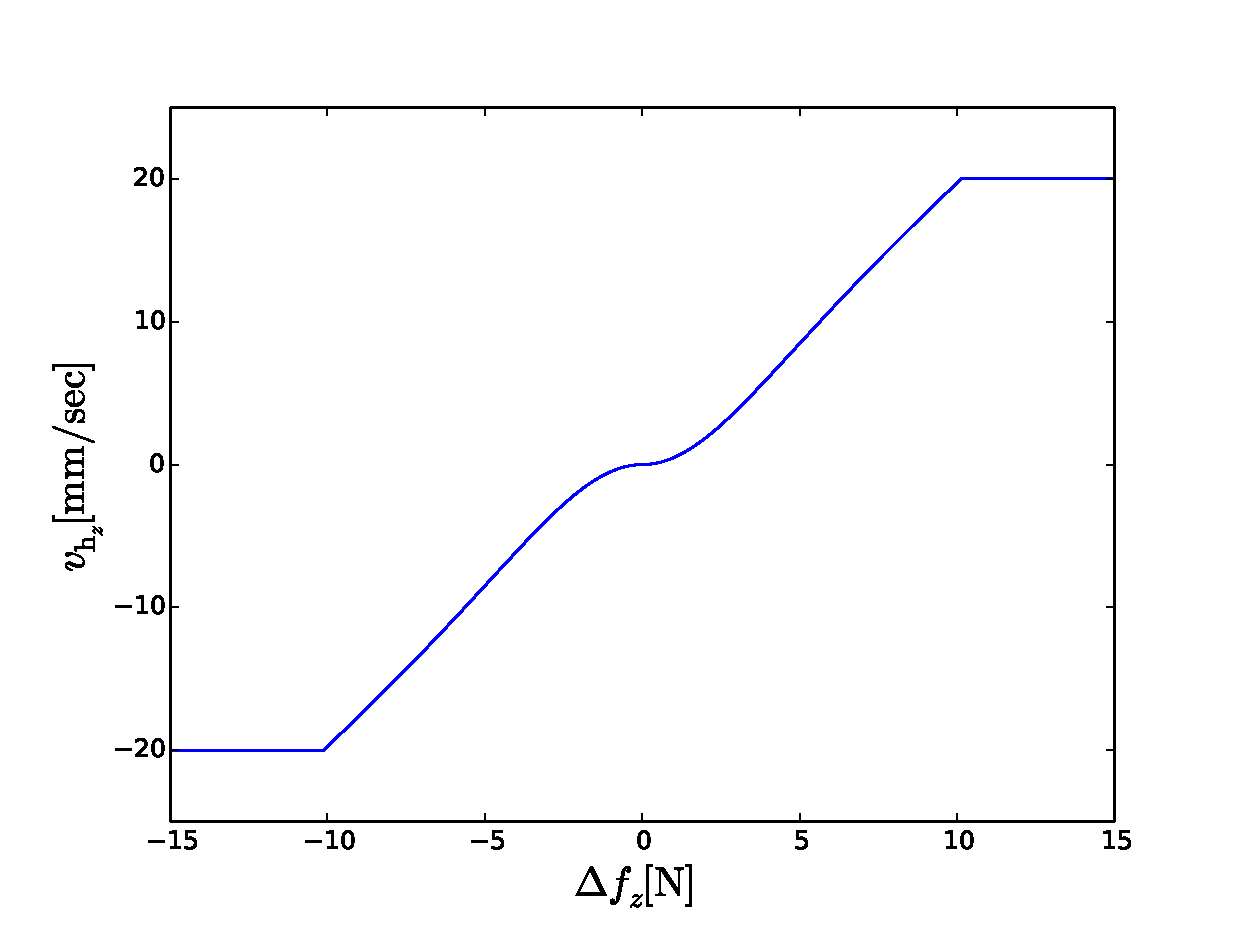
\includegraphics[width=0.75\linewidth]{fig/chp_peeling/vz_fz.eps}
  \caption{The graph of force feedback equation \ref{eq:peeling_vz}}
  \label{fig:peeling_force_feedback_graph}
\end{figure}
図\ref{fig:peeling_force_feedback_graph}で示したように，式(\ref{eq:peeling_vz})の関数の形は，基本的に $v_z$ と $f_e$ の間に線形に近い関係を持たせつつ，$f_e \approx 0$ 付近で不感帯を形成するように設計されている．
この不感帯により，微小な力計測ノイズに対する敏感な速度変動が抑制される．

\subsubsection{最低速度の設定}

実装上の課題として，式(\ref{eq:peeling_vz})では $f_e$ がゼロに近づくにつれて $v_z$ もゼロに接近するため，出力速度がロボットの動作下限を下回り，誤差が完全に収束しない現象が生じうる．
この問題を回避するため，出力速度の絶対値に最低速度 $v_{\mathrm{lim}}$ を設定する．

\begin{equation}
  v_{fz} = 
  \begin{cases}
    v_z, & \text{if}\; v_z = 0 \\[4pt]
    \mathrm{sign}(v_z)\,\max(|v_z|, v_{\mathrm{lim}}), & \text{otherwise}
  \end{cases}
  \label{eq:peeling_vz_limit}
\end{equation}

ここで，$\mathrm{sign}(v_z) = v_z / |v_z|$ は $v_z$ の符号を表す．

残りの5軸（$x$, $y$ 方向の並進および $\alpha$, $\beta$, $\gamma$ の回転）については，以下の比例制御により目標速度を生成する．

\begin{equation}
  v_i = k\,(x_{i,\mathrm{target}} - x_i),\quad i \in \{x, y, \alpha, \beta, \gamma\}
  \label{eq:peeling_position_control}
\end{equation}

ここで，$x_{i,\mathrm{target}}$ は目標位置・姿勢，$x_i$ は現在の位置・姿勢，$k$ は比例ゲインである．

\subsubsection{制御パラメータ}

今回の実験で用いられた力覚フィードバック制御のパラメータを表\ref{tab:peeling_force_params}に示す．

\begin{table}[ht]
  \centering
  \caption{The parameters of force feedback control}
  \label{tab:peeling_force_params}
  \begin{tabular}{@{}lcl@{}}
    \toprule
    Parameters & Notation & Value \\
    \midrule
    Contact force & $f_c$ & 5.0\,N \\
    Error sensitivity & $a$ & 10.0 \\
    Range of dead-zone & $b$ & 0.05 \\
    Speed min & $v_{\mathrm{lim}}$ & 0.1\,mm/s \\
    Speed max & $v_{\mathrm{max}}$ & 20.0\,mm/s \\
    \bottomrule
  \end{tabular}
\end{table}

この制御により，基準軌跡は食材形状に応じた移動方向を与え，力覚フィードバックはモデル誤差や局所的な表面凹凸を吸収する役割を担う．
すなわち，3Dモデル上の幾何学的な分析がマクロな「解」を提供し，実世界での力覚情報が微小な誤差を補償するという階層的な構造が，本手法のロバスト性の本質である．

\subsection{食材の回転操作とループ実行}
\label{sec:peeling_loop_peel_motion}

\subsubsection{食材の回転操作}

一回皮むき動作が終了し，\ref{sec:peeling_rotation_calc}で述べた手順により回転角 $\alpha$ が計算された後，食材固定側の腕が食材を回転軸 $\mathbf{v}_{\mathrm{rot}}$ 周りに角度 $\alpha$ だけ回転させる．
この回転操作により，非皮領域の隣接部がピーラー側に向き，次の一回皮むき動作の対象となる．

回転操作は，食材固定側のエンドエフェクタの回転軸周りの角度制御により実現される．
串を介して食材に回転が伝達されるため，食材と串の固定が不十分な場合には滑りが生じる可能性があるが，本実験で用いた専用エンドエフェクタ（第3章参照）により，安定した回転伝達が確保されている．

にんじんのように非皮領域の色認識が困難で，\ref{sec:peeling_rotation_calc}の回転角計算が適用できない食材については，固定回転角 $\alpha = 20^\circ$ を用いる．
この固定値は，他の食材（りんご，きゅうり，なす，じゃがいも）における回転操作回数が17〜19回の範囲に収束した実験結果に基づいて定められたものである．
すなわち，18回程度の回転で全周（$360^\circ$）をカバーするとして，$360^\circ / 18 = 20^\circ$ を固定値として採用した．

\subsubsection{終了判定}

皮むき作業の終了は，現在の食材側面における非皮領域の割合に基づいて判定する．
具体的には，非皮領域の点数 $N_{\mathrm{pe}}$ と，対象側面の全表面点数 $N_{\mathrm{side}}$ の比 $r_s$ を以下のように定義する．

\begin{equation}
  r_s = \frac{N_{\mathrm{pe}}}{N_{\mathrm{side}}}
  \label{eq:peeling_stop_ratio}
\end{equation}

この値が閾値 $r_{\mathrm{th}}$ 以上となった場合，当該側面の皮むきは十分に完了したと判断し，皮むき作業全体を終了する．

\begin{equation}
  r_s \ge r_{\mathrm{th}}
  \label{eq:peeling_stop_condition}
\end{equation}

今回の実験では，$r_{\mathrm{th}} = 0.9$ とした．

\subsubsection{反復手順}

皮むき作業の反復手順は以下の通りである．

\begin{enumerate}
  \item 食材表面点群 $P_{\mathrm{all}}$ を取得する（第3章の共通処理パイプラインによる：多視点撮影，統合，法線計算）．
  \item \ref{sec:peeling_phase_geo}節の手順により，基準軌跡 $L$ を抽出し，セグメント $s_1, s_2, \ldots, s_M$ に分割する．
  \item \ref{sec:peeling_one_peel_motion}，\ref{sec:peeling_force_feedback}項の手順により，各セグメントに沿って力覚フィードバック制御を用いながら皮むき動作を実行する（一回皮むき動作）．
  \item ピーラー側の腕を食材の上方へ移動させ，上のRGB点群を取得する．
  \item \ref{sec:peeling_rotation_calc}項の手順により，回転角 $\alpha$ を計算し，食材を回転させる（食材の回転操作）．
  \item 式(\ref{eq:peeling_stop_condition})により終了判定を行う．条件を満たさない場合は，ステップ1へ戻り，次の反復を開始する．
  \item 条件を満たした場合，皮むき作業を終了する．
\end{enumerate}

\begin{figure*}[t]
    \centering
    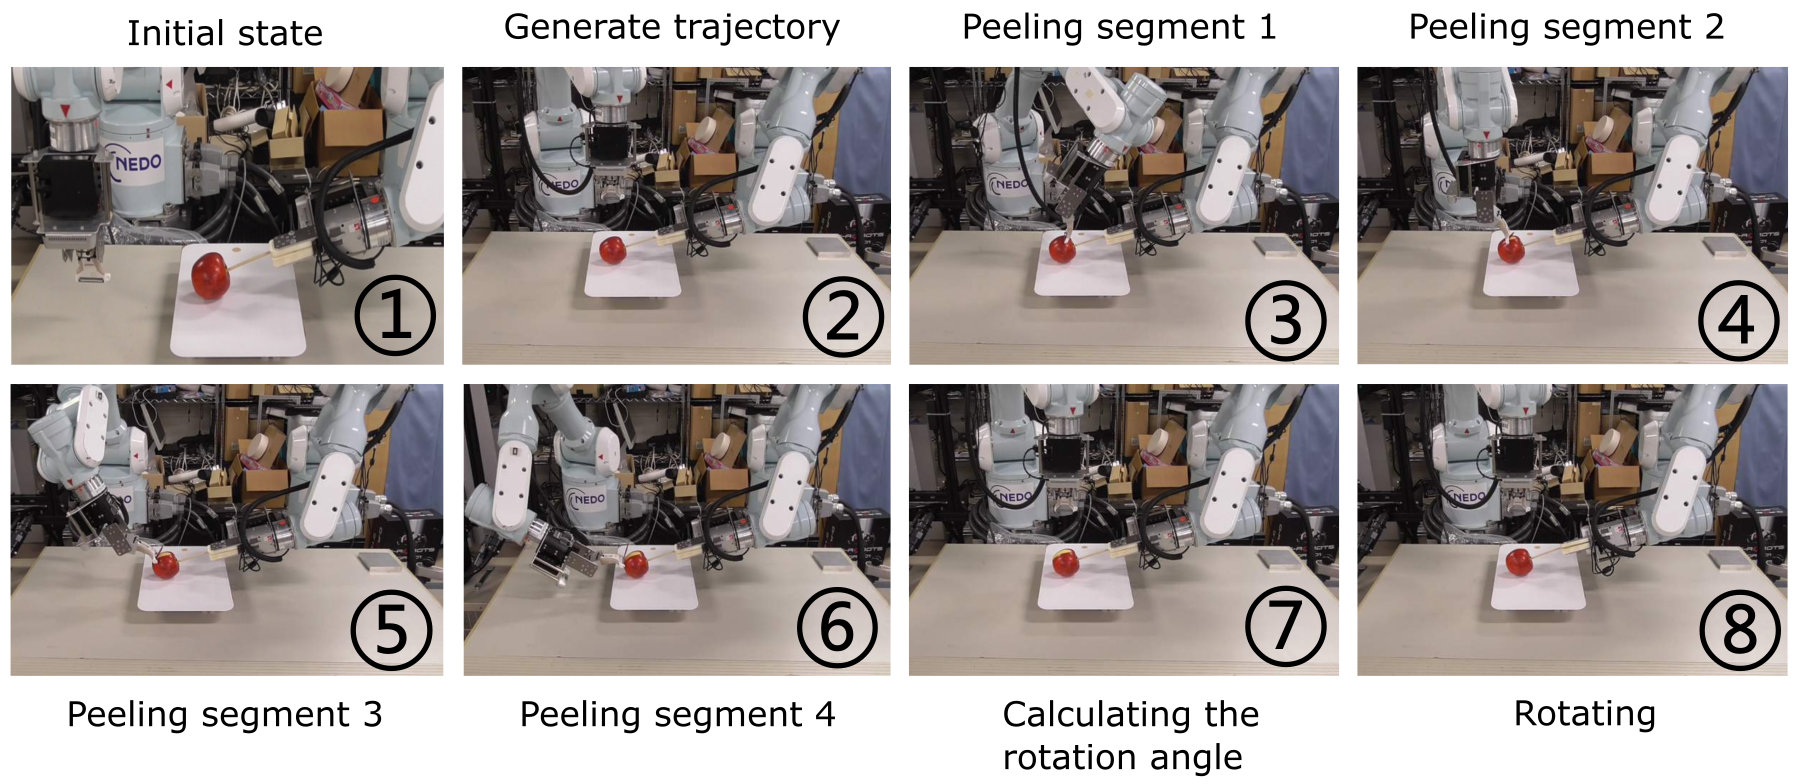
\includegraphics[width=0.95\textwidth]{fig/chp_peeling/sequence.png}
    \caption{The sequence of the proposed method. Note that if the stop condition is not satisfied, the procedure returns to step 2 while the step 8 was done.}
    \label{fig:peeling_sequence}
\end{figure*}

\section{実験}
\label{sec:peeling_phase_exp}

本節では，提案した皮むき動作生成手法を双腕ロボットシステムに実装し，複数の食材に適用する実験について述べる．

\subsection{概要}

本実験の目的は，食材表面の3D点群モデルに基づく幾何解析と，力覚フィードバック制御を組み合わせることで，形状や表面性状の異なる食材に対して皮むき動作を実現できるかを確認することである．

実験では，曲率，表面粗さ，色特徴が異なる5種類の食材を用いる．
具体的には，りんご，きゅうり，なす，じゃがいも，にんじんを対象とする．
それぞれの食材は，以下の観点から選定した．

\begin{enumerate}
  \item \textbf{りんご}：表面曲率が大きく，法線方向の変化が顕著な食材である．幾何情報に基づく軌跡生成と軌跡分割の有効性を確認する対象となる．実験では，大きさの異なる3種類（大・中・小）を各3個，計9個を用いた．りんごのサイズを表\ref{tab:peeling_apple_sizes}に示す．

  \item \textbf{きゅうり，なす}：表面曲率が比較的小さく，法線変化が緩やかな食材である．軌跡分割後のセグメント実行と接触維持の安定性を確認する対象となる．各1個を用いた．
  
  \item \textbf{じゃがいも}：表面が粗く凹凸があり，点群モデルと実表面のずれが生じやすい食材である．力覚フィードバックによる補正の有効性を確認する対象となる．1個を用いた．

  \item \textbf{にんじん}：皮と中身の色が類似しており，非皮領域の色認識が難しい食材である．RGB情報に基づく境界検出の限界を確認し，固定回転角による代替手法の有効性を検証する対象となる．1個を用いた．
\end{enumerate}

\begin{table}[ht]
  \centering
  \caption{The size of apple for experiment.}
  \label{tab:peeling_apple_sizes}
  \begin{tabular}{@{}lcc@{}}
    \toprule
    Apple & Width [mm] & Length [mm] \\
    \midrule
    Big 1 & 95.45 & 82.50 \\
    Big 2 & 95.15 & 84.40 \\
    Big 3 & 94.50 & 81.35 \\
    Medium 1 & 80.50 & 68.50 \\
    Medium 2 & 80.25 & 74.35 \\
    Medium 3 & 79.05 & 69.85 \\
    Small 1 & 53.95 & 48.85 \\
    Small 2 & 53.90 & 52.25 \\
    Small 3 & 55.05 & 46.60 \\
    \bottomrule
  \end{tabular}
\end{table}

実験では，右腕にピーラーを装着し，食材に串を刺した状態で左腕のエンドエフェクタに取り付けた．
食材の回転は，左腕の $z$ 軸周りの回転により実現した．
制御パラメータは，目標接触力 $f_c = 5.0$\,N，力誤差感度 $a = 10.0$，デッドゾーン幅 $b = 0.05$，軌跡分割閾値 $\theta_{\mathrm{th}} = 30^\circ$ とした．

ロボット本体，視覚センサ，力覚センサ，ピーラー側エンドエフェクタ，食材固定側エンドエフェクタの詳細仕様は第3章で述べているため，本節では実験目的と条件に必要な範囲に限定して記述する．

\subsection{評価指標}

皮むき結果は，非皮領域面積比 $r$ によって評価する．
実際には，面積を直接計算する代わりに点群中の点数を用いる．
これは，食材の複雑な曲面に対する面積計算を回避し，点群という本手法の基盤表現と整合的な評価を実現するためである．

評価用の点群取得にあたっては，皮むき後の食材を1視点から撮影するだけでは不可視領域のために全体の皮むき状態を把握できない．
そこで，以下の手順で評価用点群を取得する．

\begin{enumerate}
  \item 皮むき後の食材を二つに切断し，A部分・B部分とする．
  \item A部分を計測場所に置き，カメラを下方に向けて一方の側面のRGB点群 $P_A$ を取得する（点数 $N_A$）．
  \item 食材を人手で回転させ，もう一方の側面のRGB点群 $P_B$ を取得する（点数 $N_B$）．
  \item \ref{sec:peeling_rotation_calc}項と同様に，事前定義された色情報を用いて，$P_A$ から非皮領域点群 $P_{fA}$（点数 $N_{fA}$），$P_B$ から非皮領域点群 $P_{fB}$（点数 $N_{fB}$）を抽出する．
\end{enumerate}

これらの点数を用いて，皮むき率 $r$ を以下の式で計算する．

\begin{equation}
  r = \frac{N_{fA} + N_{fB}}{N_A + N_B}
  \label{eq:peeling_ratio}
\end{equation}

ここで，$r$ は非皮領域（非皮領域）の点数の，全表面点数に対する比率を表す．
すなわち，$r = 1.0$ が完全な皮むきを意味する．

\subsection{実験結果}

\begin{figure}[t]
    \centering
    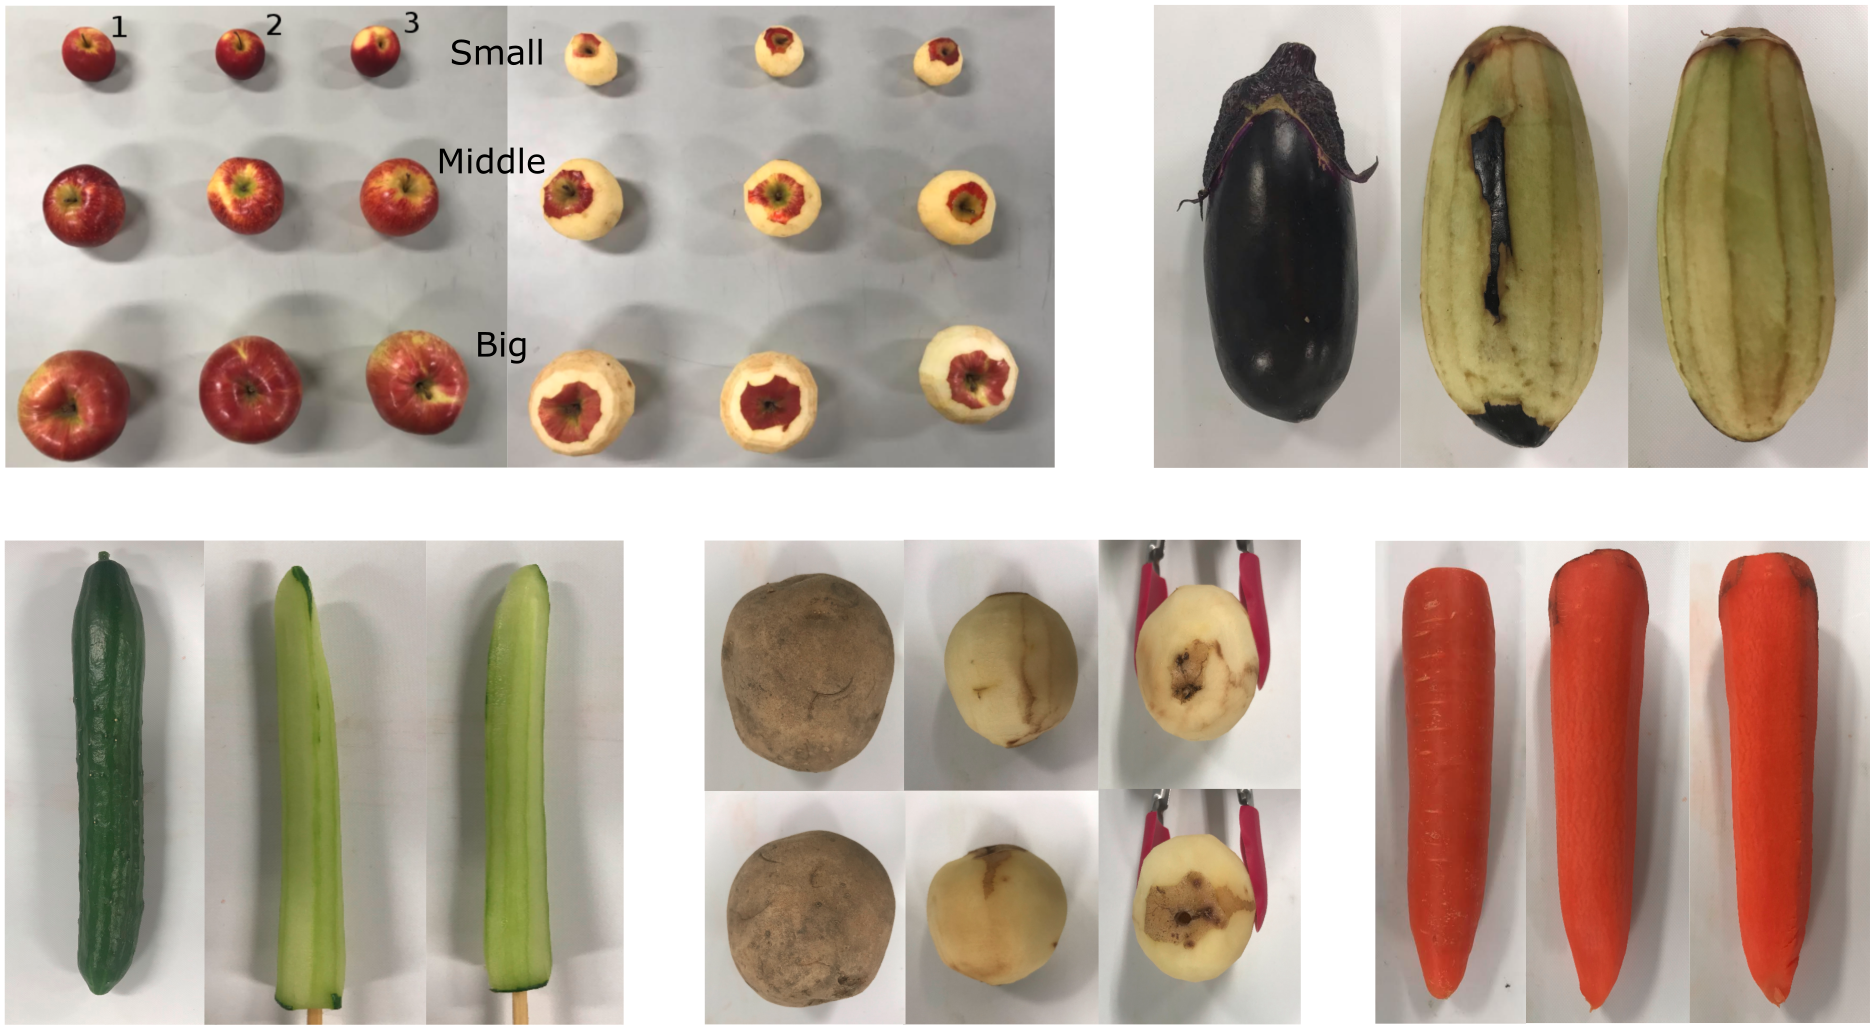
\includegraphics[width=0.7\textwidth]{fig/chp_peeling/result.png}
    \caption{The result of peeling experiment．Top left: Apples (large, medium, small); Top right: Cucumbers; Bottom left: Eggplants; Bottom middle: Potatoes; Bottom right: Carrots.}
    \label{fig:peeling_result}
\end{figure}

\subsubsection{りんご}

りんご9個（大3，中3，小3）の皮むき実験結果を図\ref{fig:peeling_result}と表\ref{tab:peeling_apple-result}に示す．

\begin{table}[t]
\centering
\caption{Peeling results for apple.}
\begin{tabular}{cccc}
	\hline
	\multirow{2}{*}{Trails} & \multicolumn{3}{c}{Ratio of the peeled area {[}\%{]}} \\ \cline{2-4} 
	& Large size     & Medium size     & Small size     \\ \hline
	1                       & 78.01          & 88.85           & 85.93          \\
	2                       & 79.83          & 84.25           & 90.93          \\
	3                       & 82.69          & 84.11           & 88.62          \\ \hline
\end{tabular}
\label{tab:peeling_apple-result}
\end{table}

りんごの結果から，全ての試行で皮むき率78\%以上を達成し，提案手法が曲率の大きな食材に対しても有効であることが確認された．
りんごの両端のくぼんだ部分は，形状的にピーラーでの皮むきが困難であり，また串に近い領域はロボットアームやエンドエフェクタとの干渉により剥きにくい．
これらの領域は，人間がりんごの皮を剥く場合にも，食べやすいサイズに切った後の段階で処理されることが多く，ピーラーで剥くことが可能な部分については提案手法で皮むきが十分に可能であることが確認された．

\subsubsection{きゅうり，なす}

きゅうり，なすの皮むき実験結果を図\ref{fig:peeling_result}と表\ref{tab:peeling_others-result}に示す．

\begin{table}[t]
\centering
\caption{Peeling results of other food. Note that the result for carrot were estimated by human eyes.}
\begin{tabular}{ccccc}
	\hline
	\multirow{2}{*}{Trails} & \multicolumn{4}{c}{Ratio of peeled area {[}\%{]}} \\ \cline{2-5} 
	& Cucumber    & Eggplant    & Potato    & Carrot    \\ \hline
	1                       & 94.31       & 90.23       & 88.72     & 95.00     \\ \hline
\end{tabular}
\label{tab:peeling_others-result}
\end{table}

きゅうり，なすのような表面の法線方向の変化が小さい食材では，りんごよりも法線のばらつきが小さいため，90\%以上の高い皮むき率が達成された．
法線変化が小さいため軌跡分割数が少なく，一つのセグメントで広範囲を安定して剥くことができたことが高い皮むき率につながったと考えられる．

なすの結果において一部の皮領域が残されたのは，終了判定のパラメータが $r_s \ge r_{\mathrm{th}} = 90\%$ と設定されており，非皮領域比率が閾値をわずかに超えた時点で作業が終了したためである．
このことから，終了判定の閾値設定が最終的な皮むき率に直接影響を与えることが確認された．

\subsubsection{じゃがいも}

じゃがいも，表面に凹凸があり，皮と中身の色が近いという二重の困難を有する食材である．
じゃがいもの結果は図\ref{fig:peeling_result}に示した．
88.72\%の皮むき率が達成されたが，芽の部分やくぼんだ部分では皮むきが十分に行われなかった．
これらの領域は，局所的に表面法線が大きく変化するため，直線セグメントによる近似では追跡しきれなかったことが原因として考えられる．

一方，表面の凹凸による点群モデルと実表面の誤差は，力覚フィードバック制御によって吸収され，全体的な接触維持は達成された．
この結果は，幾何軌跡のみでは対応できない表面粗さに対し，力覚フィードバックが有効に機能することを示している．

\subsubsection{にんじん}

にんじんは，皮と中身が同じような色をしているため，HSV色空間による非皮領域の識別が困難であった．
そのため，\ref{sec:peeling_rotation_calc}の回転角計算に代えて，固定回転角 $\alpha = 20^\circ$ を用いた．

皮むき率の評価も画像処理による自動抽出が困難であったため，目視により推定した結果，約95\%の皮むき率が得られた．
にんじんの結果は図\ref{fig:peeling_result}に示した．
固定回転角を用いた場合でも高い皮むき率が達成されたことは，$\alpha = 20^\circ$ が他の食材の回転操作回数（17〜19回）から導かれた経験的に妥当な値であることを示している．
一方で，固定回転角を用いる手法は，食材の形状や一回皮むき動作で実際に剥ける幅の変動に適応できないため，より精緻な境界認識手法の開発が今後の課題として残る．

\subsubsection{食材回転操作の回数}

各食材の皮むき作業における回転操作の回数を表\ref{tab:peeling_rotation_times}に示す．

\begin{table}[ht]
  \centering
  \caption{The times of rotation motion for each food}
  \label{tab:peeling_rotation_times}
  \begin{tabular}{@{}lcc@{}}
    \toprule
    Food &  & Rotation Times \\
    \midrule
    & Big 1 & 18 \\
    & Big 2 & 18 \\
    & Big 3 & 17 \\
    & Medium 1 & 18 \\
Apple & Medium 2 & 19 \\
    & Medium 3 & 18 \\
    & Small 1 & 18 \\
    & Small 2 & 18 \\
    & Small 3 & 17 \\
    \midrule
    Cucumber &  & 17 \\
    Eggplant &  & 18 \\
    Potato &  & 19 \\
    \bottomrule
  \end{tabular}
\end{table}

全ての食材において，回転操作回数は17〜19回の範囲に収束した．
この結果は，食材の種類や大きさによらず，一回皮むき動作で剥かれる幅と食材の全周長の比が比較的一定であることを示唆している．
この知見が，にんじんに対する固定回転角 $\alpha = 20^\circ$ の設定根拠となっている．

\subsection{考察}

考察では，結果を単に食材ごとに説明するのではなく，本章で提案した構成要素ごとに評価する．

\subsubsection{幾何情報に基づく軌跡生成の有効性}

りんごのように曲率が大きい食材では，断面輪郭に基づいて食材ごとに個別の軌跡を生成することの必要性が明確に示された．
一方，きゅうりやなすでは，法線変化が小さいため，軌跡分割後のセグメント実行が安定しやすく，94.31\%，90.23\%という高い皮むき率が達成された．

軌跡分割の閾値 $\theta_{\mathrm{th}} = 30^\circ$ は，全食材に対して共通の値で良好な結果を得たが，曲率が極端に大きい領域（例：りんごの上下端のくぼみ）では，より細かな分割が必要となる可能性がある．
適応的な閾値設定は，今後の改善方向の一つである．

\subsubsection{力覚フィードバック制御の有効性}

じゃがいものように表面が粗い食材では，点群モデルから得た軌跡と実際の接触状態の差が大きくなりやすい．
この差を力覚フィードバックが補正することで，接触を維持しながら皮むき動作を実行できた．
この結果は，本論文の「分析主導型」アプローチにおいて，幾何学的な分析（3Dモデル上の軌跡生成）と力学的制御（力覚フィードバック）の統合が有効であることを実証するものである．

なお，今回の実験では全食材に同一の制御パラメータ（$f_c = 5.0$\,N）を用いたが，食材の硬さに応じて目標接触力を調整することが，皮むき品質のさらなる向上につながると考えられる．

\subsubsection{非皮領域境界に基づく回転角計算の有効性と制限}

非皮領域を色情報により認識できる場合（りんご，きゅうり，なす），境界 $L_p$ と平均法線 $\mathbf{n}_{\mathrm{avg}}$ に基づいて次の回転角を決定する手法は有効に機能した．
特に，食材の曲率に応じて回転角が自動調整される点が，固定回転角を用いる手法に対する優位性である．

一方，にんじんのように皮と中身の色差が小さい食材では，HSV色空間による境界抽出が困難となる．
この問題に対しては，色情報以外のモダリティ（例：表面のテクスチャ変化，深層学習による領域識別）の活用が考えられる．

\subsubsection{システム上の制約と今後の課題}

串に近い領域は，ロボットアームやエンドエフェクタとの干渉により剥きにくいという構造的な制約が存在する．
これは，双腕ロボットの動作計画における到達可能性の問題であり，より多様なアプローチ方向からの皮むきや，食材把持方法の工夫が解決策として考えられる．

また，今回の実験では，皮むき作業全体の処理時間は1食材あたり約1時間を要した．
この処理時間の大部分は，点群の法線計算に費やされている．
処理時間の短縮は，実用化に向けた重要な課題である．

終了判定の閾値 $r_{\mathrm{th}} = 0.9$ によって，最大で約10\%の皮領域が残る可能性がある（なすの結果で確認された）．
この点については，終了判定基準の多角化が改善策として挙げられる．

さらに，じゃがいものような不規則形状の食材に対しては，今回の「一回皮むき＋一回回転」という反復構造では剥き残しが生じやすい．
表面法線情報に基づいて，認識された皮領域を一度に全て剥きあげた後に回転操作を実行する，といった作業構造の見直しも有効と考えられる．

\section{本章のまとめ}
\label{sec:peeling_phase_summary}

本章では，皮むき動作を対象として，第3章で得られた食材表面の3D点群モデルを入力とし，幾何情報に基づく軌跡生成と力覚フィードバック制御を統合する手法を提案・実装し，実験によりその有効性を検証した．

本章の主要な成果を以下に要約する．

\begin{enumerate}
  \item \textbf{皮むき動作の定式化}：ピーラー操作が「一回皮むき動作」と「食材の回転操作」に自然に分解されることに着目し，皮むき動作を双腕ロボット上で実装可能な形に定式化した．

  \item \textbf{幾何情報に基づく軌跡生成}：食材の回転軸を含み作業台平面に垂直な断面抽出平面 $\mathcal{P}_{c1}$ により断面輪郭 $L_c$ を抽出し，到達可能性判定平面 $\mathcal{P}_{c2}$ により下側部分を除去することで，到達可能な基準軌跡 $L$ を生成した．さらに，表面法線の変化に基づいて軌跡を複数のセグメント $s_j$ に分割し，ピーラー刃の受動的回転機能と相まって，実機での安定な直線実行を可能とした．

  \item \textbf{力覚フィードバック制御の統合}：軌跡追跡のための位置制御と，接触維持のための力制御を統合したハイブリッド制御構造を採用した．力制御には，目標接触力 $f_c$ と実測値 $f_s$ の誤差に基づく速度補正式（式(\ref{eq:peeling_vz})）を用い，最低速度 $v_{\mathrm{lim}}$ の設定により誤差収束の停滞を防止した．これにより，最終的にロバストな皮むき動作が実現された．

  \item \textbf{非皮領域に基づく回転角の計算}：RGB情報とHSV色空間を用いて非皮領域を抽出し，その境界 $L_p$ 近傍の平均法線 $\mathbf{n}_{\mathrm{avg}}$ と基準ベクトル $\mathbf{v}_{\mathrm{ref}}$ のなす角から次回の回転角 $\alpha$ を計算する手法を提案した．この手法により，食材の曲率に応じた適応的な回転角の決定が可能となった．色認識が困難な食材に対しては，固定回転角 $\alpha = 20^\circ$ による代替手法を併用した．

  \item \textbf{実機実験による検証}：りんご（9個），きゅうり，なす，じゃがいも，にんじんの合計13個の食材を用いた実機実験を実施し，全ての食材で皮むき率78\%以上を達成した．特に，きゅうり（94.31\%），なす（90.23\%），にんじん（95.00\%）では90\%以上の高い皮むき率が得られ，提案手法が形状，曲率，表面粗さ，および色特徴の異なる対象に対して適用可能であることを検証した．
\end{enumerate}

以上の結果から，3D点群モデルに基づく幾何学的な分析と力覚フィードバック制御の統合が，個体差の大きい食材の皮むき動作に対して有効なアプローチであることが示された．
本成果は，第1章で提案した「分析主導型」アプローチの具体的な実証例として位置づけられる．

次章では，対象表面へ直接工具を接触させる本章の操作から，直接把持できない液体を容器を介して操作する課題へ移る．容器の3D幾何から体積と注ぎ角度を計算することで，環境的な分析と幾何学的な分析を動作制御へ接続する．
	\chapter{タスク2：液体を注ぐ作業}
\label{ch:pour}
% ============================================================================

本章では，第\ref{ch:introduction}章で示した形状および環境・道具の分析観点を，
料理作業において高い頻度で現れる「注ぐ」動作に適用する．
注ぎ作業は，直接把持できない液体を対象とし，容器という環境を介して間接的に操作する点に
特徴がある．したがって，本作業は第\ref{ch:introduction}章の表\ref{tab:tasks}に示した
「容器間関係（環境的な分析）」と「容積・形状（幾何学的な分析）」の検証に位置づけられる．

本章では，第\ref{ch:system}章で構築した容器の3D点群モデルを基盤とし，
幾何学的な分析による注いだ体積の推定と，動作制御による精密な注ぎ実行を統合することで，
\revise{事前登録していない形状の容器に対して，容器形状を液体量または目標角度へ変換し，制御中に計量カップや秤を用いない定量注ぎを実現する二つのタスク固有手法を提案する．}

本章の構成は以下の通りである．
まず\ref{sec:pour_problem_overview}節で注ぎ作業の問題設定と提案手法の全体像を述べる．
次に\ref{sec:pour_analysis}節では，本手法のコアとなる幾何学的な分析として，
液面検出による注いだ体積の推定，注ぎ口形状の認識，および注ぎ角度と注いだ量の関係の計算について
述べる．
\ref{sec:pour_control}節では，分析結果に基づく動作制御として，
注いだ液体の量でフィードバックし，注ぐ容器の回転角速度のPD制御と注ぐ容器の回転角度のP制御
の2つの制御手法を述べる．
\ref{sec:pour_experiment}節では，形状特性の異なる複数容器を用いた実験により
提案手法の有効性を検証する．
最後に\ref{sec:pour_summary}節で本章を総括する．


% ============================================================================
\section{問題設定と提案手法の概要}
\label{sec:pour_problem_overview}
% ============================================================================

\begin{revisionblock}
\subsection{想定する状況，目的および適用条件}
本章は，家庭の調理中に，水，牛乳，だし等の低粘性液体を一つの開口容器から別の開口容器へ指定量だけ移す状況を想定する．
ロボットには注ぐ操作，使用する二容器，目標体積 $V_{\mathrm{tar}}$，および把持方法が与えられており，対象容器の形状に応じた液量または傾斜角度が未決定である．
液体・容器の選択，レシピからの目標量抽出，容器の初期配置，こぼれ後の清掃，および複数工程の切替えは対象外とする．

手法1では注ぎ先容器の内面と注ぎ中の液面を観測できること，手法2では注ぐ容器の形状と初期液体体積が得られることを前提とする．
両手法とも，容器を剛体，液体を水・牛乳程度の低粘性流体とし，注ぎ先への流れが遮られない状況を扱う．
本章の達成目標は，容器ごとの事前登録モデルなしに，その場で得た容器形状から液面高さ・体積関係または傾斜角度・流出量関係を求め，設定した条件下で指定量を注ぐことである．
\end{revisionblock}

\subsection{注ぎ作業の定式化と技術的課題}

料理作業において，注ぎ作業は液体調味料（酢，醤油など）の投入や水の添加など，
高い頻度で現れる基本操作である．
レシピに示された分量通りに定量的に注がなければ，料理の味や食感が変わってしまうため，
注ぐ量の定量性は調理の成否に直結する．

人間が定量的な注ぎを行う場合，計量カップ，計量スプーン，あるいは秤を用いて
液体の体積を計量するのが一般的である．
しかし，このような道具を用いる方法では，正確な分量を計量できる反面，
計量作業を別途実施しなければならないという問題がある．
例えば，水を複数のコップに均等に分ける場合，容器ごとに体積を計量する必要があるため，
作業時間が増大する．
\begin{revisionblock}
ロボットが容器形状を直接計測して液体体積を計算できれば，計量専用容器への移替え，追加の把持・搬送，および使用後の洗浄を省き，注ぎ先容器へ直接移すことができる．
また，同一液体を複数容器へ分配する場合には，各容器を秤へ移動することなく連続して作業できる．
一方，計量カップや秤は既に簡便で高精度な手段であり，本研究はそれらが不要であることを主張するものではない．
本手法の利点は，既存の視覚・操作系だけで容器形状を制御量へ変換し，補助器具と作業工程を減らせる点にあり，必要精度，観測可能性，清掃性に応じて従来の計量手段と使い分けるべきである．
\end{revisionblock}

したがって，本研究で解決すべき課題は次のように定式化される：

\begin{quote}
  事前に形状が未知である注ぐ容器から，
  同じく形状が未知である注ぎ先容器へ，
  計量カップや秤などの外部計測道具を用いることなく，
  指定された目標体積 $V_{\mathrm{tar}}$ の液体を精密に注ぐこと．
\end{quote}

この課題を実現するためには，以下の2つの中核的課題を解決する必要がある：

\begin{description}
  \item[課題1] 注いだ体積の測定．
    注いだ体積が不明であれば「定量的」とは言えない．
    したがって，注いだ体積の測定は本研究の中心であり，
    \revise{対象容器ごとの事前モデルに依存せず，その場で計測した形状から体積を求められる方法が必要となる．}
  \item[課題2] 注ぎ動作の制御．
    注いだ体積が推定できたとしても，注ぎ動作の制御が高精度に行えなければ，
    液体がこぼれたり，一気に大量の液体が注いだりする可能性がある．
    これは誤差の原因となるため，注いでいる間における注ぐ容器の傾き角度の制御が重要である．
\end{description}


\subsection{提案手法の概要}

上記の2つの課題に対し，注ぎ作業には注ぐ容器と注ぎ先容器の2つの容器が関連することから，
本研究ではそれぞれの容器に着目した2つの方法論を提案する．

\begin{enumerate}
  \item \textbf{手法1：注ぎ先容器に注目} 
    　注ぎ先容器の3Dモデルと，注いでいる間にリアルタイム検出される液面高さから
    現在注いだ体積を推定する．その体積誤差に基づくPD制御により
    注ぐ容器の傾き角速度を操作する方法である．
    この手法の利点は，注ぐ容器の状態や形状が未知であっても正確に注げる点にあるが，
    注ぎ先容器の内部形状が計測できない場合には適用できない．
  
  \item \textbf{手法2：注ぐ容器に注目} 
    　注ぐ容器の3Dモデルと初期液体の量から注ぎ口形状を認識し，
    容器の傾き角度と注いだ体積の関係を事前に計算する．
    この関係に基づき，目標体積に対応する目標角度まで注ぐ容器を回転させる
    P制御により注ぎを実行する方法である．
    この手法は手法１の欠点（注ぎ先容器の内部計測不能時）を補完できる一方，
    注ぐ容器の形状と初期液体の量が計測できない場合には適用できない．
\end{enumerate}

2つの手法を合わせて使用することで，注ぐ容器か注ぎ先容器のどちらか一方の
3Dモデルが取得可能であれば，注いだ体積の測定と動作制御が可能となる．

両手法に共通する基盤として，第\ref{ch:system}章で述べた手順により
容器の3D点群モデルを事前に取得する．
また，容器モデルからの部分容積計算についても第\ref{ch:system}章の
スライス断面積積分に基づく手法を前提とするが，
本章では特に，任意の液面高さ $H$ および容器姿勢 $\theta$ における
容器下部の体積 $V_{H,\theta}$ を，

\begin{equation}
  V_{H,\theta} = \int_{0}^{H} S(h,\theta)\,dh
  \label{eq:pour_volume_integral}
\end{equation}

と表す．
ここで $S(h,\theta)$ は，容器モデルを高さ $h$ の水平面で切断したときの断面積であり，
容器の傾き角度 $\theta$ に依存する関数である．
式(\ref{eq:pour_volume_integral})の離散化計算は，
モデルを $z$ 軸に沿って高さ $h_\delta$ の $N$ 個の部分に分割し，
各部分の体積 $V_n$ を上下断面積の台形近似により求め，
それらの総和として計算する：

\begin{equation}
  V_n \approx \frac{(S_{n-1} + S_n)\,h_\delta}{2}, \quad
  V_{H,\theta} = \sum_{n=1}^{N} V_n
  \label{eq:pour_volume_discrete}
\end{equation}

ここで $h_\delta = H/N$，$S_n = S(h_\delta \cdot n,\;\theta)$ である．
各断面の面積 $S_n$ は，スライス断面に含まれる点群をスライス平面に投影した後，
ConvexHull を用いて計算する．

% -------------------- IROS2019 Fig. ParametersV4 --------------------
\begin{figure}[t]
	\vspace{3mm}
	\centering
	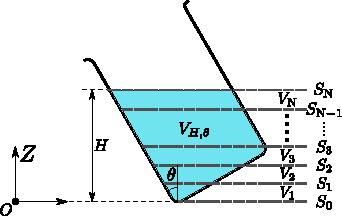
\includegraphics[width=.8\linewidth]{fig/chp_pouring/ParametersV4.pdf}
	\caption{
		$V_H$ is the volume that we want to calculate.
		$H$ is the height, and can be set between the bottom of the model and top of the model.
		To calculate the integration, $S_0, S_1, S_2, \dots, S_N$ are the areas of each cross-sectional plane. $V_1, V_2, V_3, \dots, V_N$ are the volumes of each slice part.}
	\label{fig:pour_ParametersV4}
\end{figure}
% -------------------------------------------------------------------


% ============================================================================
\section{注ぎ作業のための幾何学的な分析}
\label{sec:pour_analysis}
% ============================================================================

本節では，提案手法の幾何学的な分析として，
注ぎ先容器を対象とした液面検出に基づく注いだ体積のリアルタイム推定
（\ref{sec:pour_liquid_level}節），
注ぐ容器を対象とした注ぎ口形状の認識（\ref{sec:pour_edge_point}節），
注ぎ角度と注いだ体積の関係計算（\ref{sec:pour_angle_volume}節）
について述べる．

% ---------------------------------------------------------------------------
\subsection{液面による注いだ体積の推定}
\label{sec:pour_liquid_level}
% ---------------------------------------------------------------------------

手法1では，注いでいる間に注ぎ先容器内の液面をリアルタイムで検出し，
その高さから現在注いだ体積を推定する必要がある．
醤油や酢，油などの料理によく使われる液体は流動性が高く，
大きな外力が加わらない限り液面は常に水平面と平行になる．
この特性を利用し，注ぎ先容器モデルの底面から液面までの間の体積を
注がれた液体の体積とみなす．

\subsubsection{RANSAC による液面検出}

液面検出は，注いでいる間にカメラから取得される各フレームの点群に対して
以下の手順で行う．

\begin{enumerate}
  \item 事前に計算した注ぎ先容器のAABBを用いて，
        PassThroughフィルタにより容器外部の点を除去し，
        容器内部近傍の点群のみを抽出する．
  \item 抽出された点群に対し，RANSACを適用し，
        最も多くのインライアが得られる平面を検出する．
  \item 検出された平面を液面とみなし，その高さ $H_{\mathrm{liquid}}$ を
        容器底面を基準とする座標系での $z$ 座標値として取得する．
\end{enumerate}

RANSAC による平面検出を用いれば，液面以外の構造（容器側壁，底面，ノイズ点）が
混在する点群からでも，液面を安定に抽出できるため，本作業に適している．

\subsubsection{液面高さから注いだ体積への変換}

検出された液面高さ $H_{\mathrm{liquid}}$ を用いて，
現在注いだ体積 $V_{\mathrm{pour}}$ は式(\ref{eq:pour_volume_integral})により
以下のように計算される：

\begin{equation}
  V_{\mathrm{pour}} = V_{H_{\mathrm{liquid}},\,\theta_{\mathrm{target}}}
  = \int_{0}^{H_{\mathrm{liquid}}} S(h,\theta_{\mathrm{target}})\,dh
\end{equation}

ここで $\theta_{\mathrm{target}}$ は注ぎ先容器の傾き角度であり，
注いでいる間は一定と仮定する．
これにより，各制御ステップにおいて現在注いだ体積 $V_{\mathrm{now}}$ が得られ，
目標体積 $V_{\mathrm{tar}}$ との誤差

\begin{equation}
  V_{\mathrm{error}} = V_{\mathrm{tar}} - V_{\mathrm{now}}
  \label{eq:pour_verror}
\end{equation}

がPD制御への入力として用いられる．

% ---------------------------------------------------------------------------
\subsection{注ぐ容器の注ぎ口形状の認識}
\label{sec:pour_edge_point}
% ---------------------------------------------------------------------------

手法2では，注ぐ容器を傾けた際に液体が流出する「注ぎ口」の幾何学的特徴を
事前に求める必要がある．
注ぎ口の認識は，(a) 注ぎ縁の検出と，(b) 注ぐポイントの検出，
の2段階で構成される．

\subsubsection{注ぎ縁の検出}

注ぎ縁とは，容器内部から外部へと通じる開口部の縁である．
容器をスライスしたとき，注ぎ縁を含む断面には必ず不連続な部分が生じる．
この不連続部分の端点を集めることで，注ぎ縁を検出できる．

具体的な検出手順を以下に示す．

\begin{enumerate}
  \item 容器モデルに対し，複数の変換行列 $\mathbf{T}_k\;(k=1,\dots,K)$ を適用し，
        異なる姿勢での点群を生成する．
  \item 各姿勢において，モデルを $z$ 軸方向に1\,mm間隔でスライスし，
        各スライス断面の点群を取得する．
  \item 各断面点群に対し，PCL の ConvexHull モジュールを用いて凸包を計算する．
        ConvexHull の結果は順序付けられた配列で得られるため，
        断面形状に沿った隣接点関係が定まる．
  \item ConvexHull 上の隣接する2点に対し，
        その2点を結ぶ直線から半径 $r = 2.5\,\mathrm{mm}$ 以内にある
        内部点を抽出し，直線上に投影する．
  \item 投影点間の距離を計算し，距離が閾値 $D_T = 2.5\,\mathrm{mm}$ より
        大きい点対を不連続部分の端点として検出する．
  \item 検出された端点群を逆変換 $\mathbf{T}_k^{-1}$ により
        元のモデル座標系へ戻し，全姿勢の結果を統合して注ぎ縁点群を得る．
\end{enumerate}

% -------------------- IROS2019 Fig. pour-edge-1 and pour-edge-2 --------------------
\begin{figure}[t]
	\vspace{3mm}
	\centering
	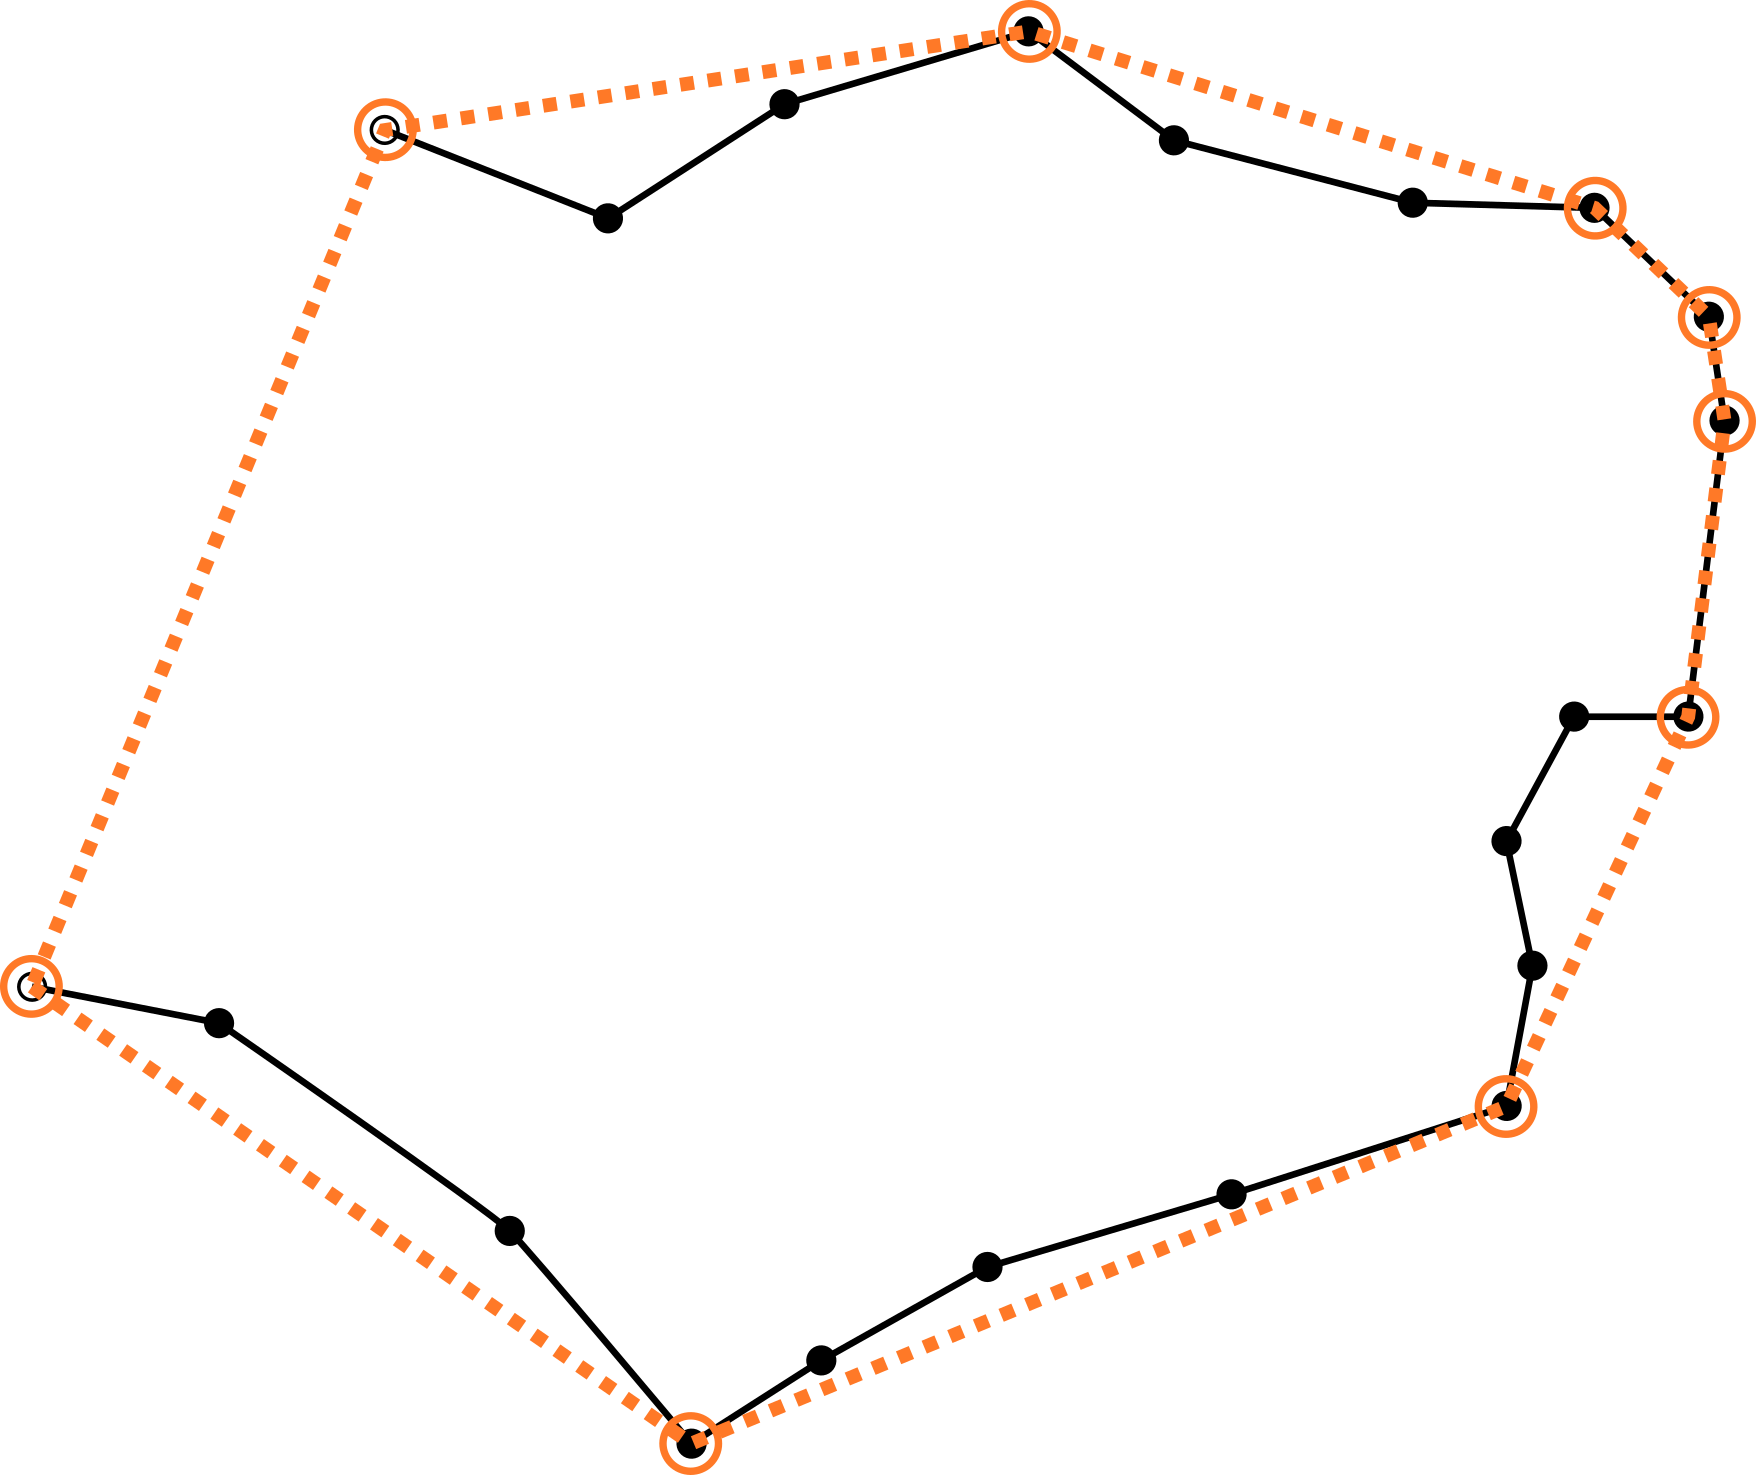
\includegraphics[width=0.57\linewidth]{fig/chp_pouring/PourEdgeConvexHull.png}
	\caption{
		Black points are the cross-sectional point set.
		Black circles mark the endpoints that need to be found.
		Points surrounded by orange circles are the results of \cite{PCL-Convex}, and these points are stored in an ordered array (marked with an orange broken line).
	}
	\label{fig:pour_pour-edge-1}
\end{figure}

\begin{figure}[t]
	\vspace{3mm}
	\centering
	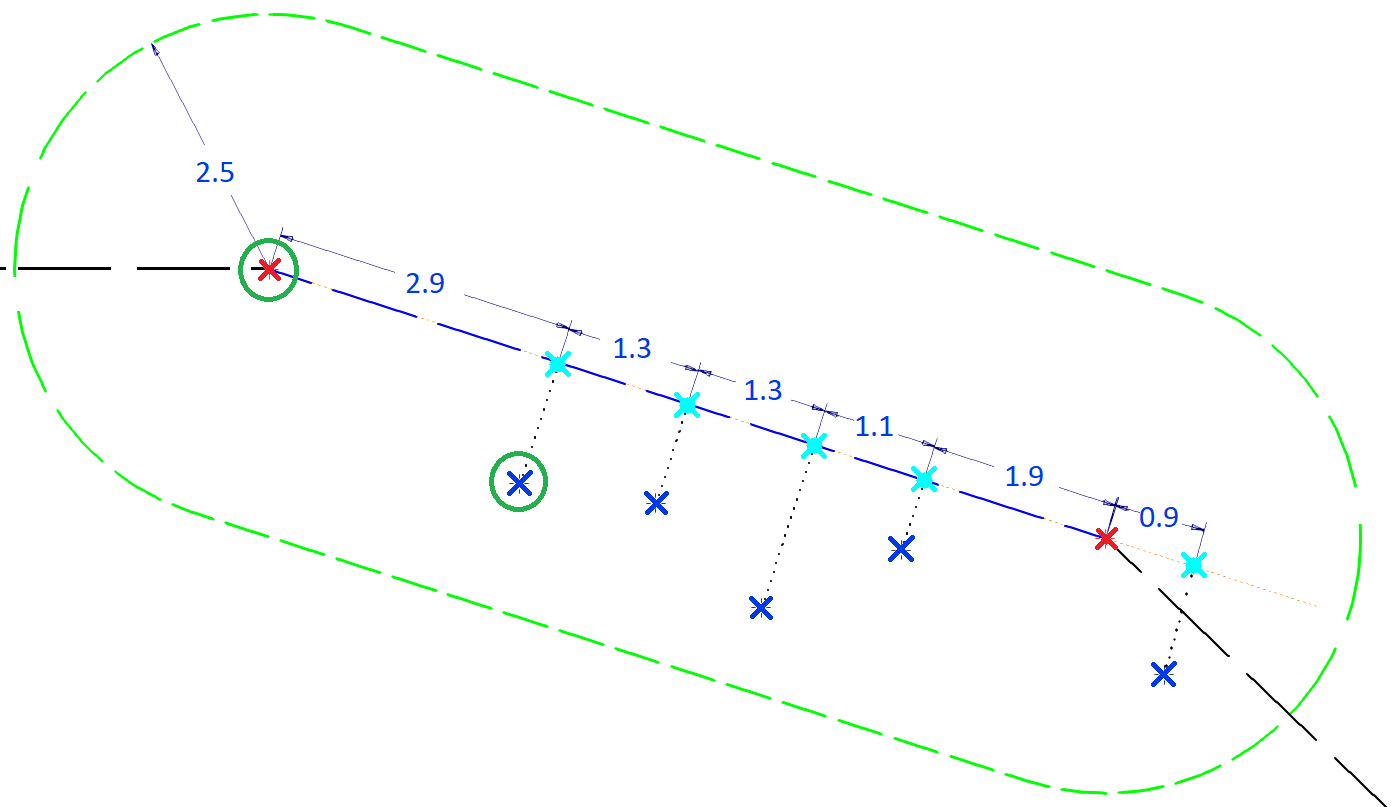
\includegraphics[width=0.9\linewidth]{fig/chp_pouring/pour-edge-2.png}
	\caption{
		This figure shows the point and its neighbor on the convex hull.
		Blue and black broken lines and red crosses are the results of the convex hull. Black broken lines are not related to the endpoints analysis.
		The green broken line is the border of points that will be analyzed.
		Deep blue crosses mark the inner points of the cross-sectional shape.
		Cyan crosses mark the inner points that will be projected onto the line defined by the two red crosses.
		Two points surrounded by deep green circles are the resulting endpoints.}
	\label{fig:pour_pour-edge-2}
\end{figure}
% --------------------------------------------------------------------------------

検出された注ぎ縁にはノイズが含まれるため，
PCLのEuclideanClusterExtractionを用いてクラスタリングし，
平均高さと点数が最大のクラスタを最終的な注ぎ縁として採用する．

\subsubsection{注ぐポイントの検出}

注ぎ縁が得られた後，実際に液体が流出する「注ぐポイント」$\mathbf{P}_{\mathrm{pour}}$
を検出する．
凸形状容器において，注ぐポイントは注ぎ縁の最下点として定義される．

検出手順は以下の通りである：

\begin{enumerate}
  \item 注ぎ縁点群を $x$ 軸回りに複数の傾き角度に回転変換し，
        各姿勢における最下点（$z$ 座標が最小の点）を抽出する．
  \item 全姿勢から得られた最下点群を変換行列により統合する．
  \item 統合された点群に Euclidean クラスタリングを適用し，
        平均高さが最も低いクラスタの重心をもって
        注ぐポイント $\mathbf{P}_{\mathrm{pour}}$ とする．
\end{enumerate}

このように，複数姿勢からの投票に基づく手法により，
単一視点では判断が難しい注ぎ口の最下点を安定して検出できる．

% ---------------------------------------------------------------------------
\subsection{注ぎ角度と注いだ体積の関係計算}
\label{sec:pour_angle_volume}
% ---------------------------------------------------------------------------

注ぐポイント $\mathbf{P}_{\mathrm{pour}}$ が検出されると，
注ぐ容器の傾き角度 $\theta$ と注いだ体積 $V_{\mathrm{pour}}$ の関係を計算できる．
本計算では以下の仮定をおく：

\begin{enumerate}
  \item 注ぎの過程で液こぼれはなし（注いだ液体はすべて注ぎ先容器に注いだ）．
  \item 注ぐ容器内の初期液体体積 $V_{\mathrm{init}}$ は既知である．
  \item $V_{\mathrm{init}} > V_{\mathrm{tar}}$，すなわち初期液体体積は目標体積より十分に大きい．
  \item 液体の粘性は低く（水，ミルク程度），液体は容器の形状に沿って変形する．
  \item 表面張力の影響はここでは無視できるものとする．
\end{enumerate}

% -------------------- IROS2019 Fig. Pouring --------------------
\begin{figure}[t]
	\vspace{3mm}
	\centering
	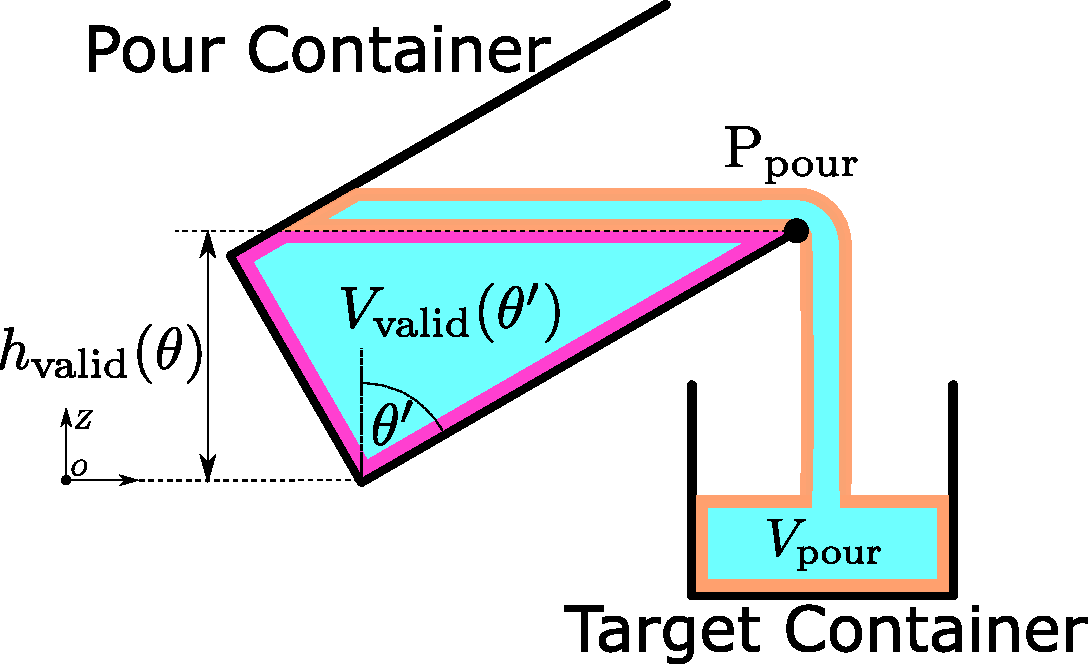
\includegraphics[width=0.7\linewidth]{fig/chp_pouring/Pouring.pdf}
	\caption{
		This figure depicts the pouring scenario when the angle of the pouring container $\theta$ is $\theta^\prime$.
		$\theta^\prime$ is the angle at which the liquid pours out from the pouring container, so $V_\mathrm{valid}(\theta^{\prime})$ (purple frame) is the volume that rests in the pouring container.
		$h_\mathrm{valid}(\theta)$ is defined as the height between the pouring point $\mathrm{P}_\mathrm{pour}$ and the bottom of pouring container.
		$V_\mathrm{pour}$ is the poured volume.
	}
	\label{fig:pour_Pouring}
\end{figure}
% ------------------------------------------------------------

注ぐポイント $\mathbf{P}_{\mathrm{pour}}$ から容器モデル最下点までの
$z$ 軸方向距離を $h_{\mathrm{valid}}(\theta)$ と定義する．
これは傾き角度 $\theta$ の関数であり，$\theta$ における注ぎ口の有効高さを表す．

注ぎ開始前（$\theta = 0^\circ$）の時点では，
$V_{\mathrm{valid}}(0^\circ)$ は容器の最大容積を表し，
$V_{\mathrm{init}}$ はこの容器内に実際に存在する液体の体積である．

注いでいる間の任意の傾き角度 $\theta$ において，
容器内に残された液体の体積 $V_{\mathrm{rest}}$ は常に
$V_{\mathrm{valid}}(\theta)$ と一致する．
すなわち：
\begin{equation}
  V_{\mathrm{valid}}(\theta) = \int_{0}^{h_{\mathrm{valid}}(\theta)} S(h,\theta)\,dh
  = V_{\mathrm{rest}}
\end{equation}

また，注いでいる間，注ぐ容器の液面高さと注ぐポイントの高さは等しく，
かつ注ぐ容器から流出した体積はすべて注ぎ先容器に注がれた体積に等しいという
2つの条件から，
$V_{\mathrm{init}}$，$V_{\mathrm{rest}}$，$V_{\mathrm{pour}}$ の関係は：

\begin{equation}
  V_{\mathrm{init}} = V_{\mathrm{rest}} + V_{\mathrm{pour}}
  = V_{\mathrm{valid}}(\theta) + V_{\mathrm{pour}}
  \label{eq:pour_volume_relation}
\end{equation}

と表される．

したがって，傾き角度 $\theta$ における注いだ体積 $V_{\mathrm{pour}}(\theta)$ は，
以下の式で与えられる：

\begin{equation}
  V_{\mathrm{pour}}(\theta) = 
  \begin{cases}
    0 & \bigl(V_{\mathrm{valid}}(\theta) > V_{\mathrm{init}}\bigr) \\[6pt]
    V_{\mathrm{init}} - V_{\mathrm{valid}}(\theta) & \text{その他}
  \end{cases}
  \quad (0^\circ \leq \theta \leq 180^\circ)
  \label{eq:pour_angle_volume_relation}
\end{equation}

一つ目の場合は，液面がまだ注ぐポイントに到達しておらず，
液体が流出していない状態に対応する．

% ---------------------------------------------------------------------------
\subsection{リアルタイム処理のための変換テーブル}
\label{sec:pour_transform_table}
% ---------------------------------------------------------------------------

\subsubsection{液面高さ→注いだ体積変換テーブル}

手法1の実行時，断面積積分をリアルタイムで毎回計算することは計算負荷が高い．
そこで，容器モデル取得時に，液面高さ $h$ から注いだ体積 $V$ への
変換テーブル $T(h)$ を事前に作成しておく．

具体的には，容器底面 $z_{\mathrm{min}}$ から上面 $z_{\mathrm{max}}$ まで
1\,mm 刻みで各高さ $h_i$ に対応する体積 $V_{h_i}$ を
式(\ref{eq:pour_volume_discrete})により計算し，テーブルとして格納する．
注いでいる間に液面高さ $h$ が検出された際には，テーブル参照と線形補間により
注いだ体積を得る：

\begin{equation}
  V_{\mathrm{output}} = T(\lfloor h \rfloor) 
  + \bigl(T(\lceil h \rceil) - T(\lfloor h \rfloor)\bigr)
  \cdot \bigl(h - \lfloor h \rfloor\bigr)
  \label{eq:pour_table_interp}
\end{equation}

これにより，注いでいる間の計算コストを大幅に低減し，
高い制御周期を維持することが可能となる．

\subsubsection{傾き角度→注いだ体積変換テーブルのノイズ処理}

手法2についても，\ref{sec:pour_angle_volume}節の方法で
傾き角度 $\theta$ から注いだ体積 $V_{\mathrm{pour}}$ への変換テーブルを作成する．
しかし，点群モデルのノイズの影響により，角度の増加に伴って
計算上の注いだ体積が一時的に減少する現象が生じる場合がある．
これは，実際には角度増加時に注いだ体積が減少することはありえないため，
誤差の原因となる．

この問題に対し，変換テーブルにおいて注いだ体積の減少が検出された区間では，
線形補間を用いてデータを補正する．
具体的には，減少開始点と減少終了点の間を直線で補間することで，
単調増加性を保証したテーブルを得る．

さらに，注ぎ実行時には目標体積から目標角度を逆引きする必要があるため，
注いだ体積から傾き角度への逆変換テーブルをバイナリサーチにより作成する．
これにより，目標体積 $V_{\mathrm{tar}}$ に対応する目標角度 $\theta_{\mathrm{tar}}$ が
$O(\log N)$ で探索可能となる．


% ============================================================================
\section{動作制御}
\label{sec:pour_control}
% ============================================================================

前節の幾何学的な分析により得られた注いだ体積の推定に基づき，
本節では2つの手法のための実際にロボットの注ぎ動作の制御について述べる．
いずれの手法においても，注ぎ動作は「傾き制御」と注ぎ停止後の「戻し動作」の
2つの段階で構成される．

% ---------------------------------------------------------------------------
\subsection{手法1の制御：注いだ体積積をフィードバックするPD制御}
\label{sec:pour_method1_pd_control}
% ---------------------------------------------------------------------------

手法1では，\ref{sec:pour_liquid_level}節で述べた液面検出により
リアルタイムに推定される注いだ体積をフィードバックとして，
注ぐ容器の傾き角速度 $\omega$ をPD制御により操作する．

\subsubsection{PD制御則の設計}

注ぎ作業において，一度注がれた液体は注ぐ容器に戻らないという特性がある．
このため，体積誤差 $V_{\mathrm{error}}$（式(\ref{eq:pour_verror})）の積分項は
常に増大し続け，目標値に達しても注ぎを継続する方向に作用してしまう．
したがって，I制御を含むPID制御は本作業に不向きであり，
積分項を省略したPD制御を採用する．

制御則は以下の通りである：

\begin{equation}
  \omega = k_p\,V_{\mathrm{error}} + k_d\,D_{\mathrm{error}}
  \label{eq:pour_pd_control}
\end{equation}

ここで $k_p$ は比例ゲイン，$k_d$ は微分ゲインであり，
$D_{\mathrm{error}}$ は注いだ体積の増加速度（体積誤差の時間微分）である．

また，$V_{\mathrm{error}}$ が大きい初期段階において，
式(\ref{eq:pour_pd_control})の $\omega$ をそのまま適用すると
一気に大量の液体が注がれてしまう可能性がある．
これを防止するため，角速度 $\omega$ に上下限制約を設ける．
本研究では $-2^\circ/\mathrm{s} \leq \omega \leq 2^\circ/\mathrm{s}$ と設定した．

\subsubsection{停止条件と戻し動作}

注ぎ動作の停止条件は，体積誤差がゼロ以下になった時点とする：

\begin{equation}
  V_{\mathrm{error}} \leq 0
  \label{eq:pour_stop_condition}
\end{equation}

停止条件が満たされた後，液体の増加を可能な限り速やかに停止させるため，
直ちに戻し動作を実行する．
戻し動作では，PDコントローラを停止し，手先座標系を $\omega$ の負の方向に回転させ，
注ぐ容器がテーブルに対して垂直になるまで戻す．
これにより，注ぎ口からの液体の流出を速やかに止め，
目標体積を超える量が注がれるのを防ぐ．

% ---------------------------------------------------------------------------
\subsection{手法2の制御：目標角度をフィードバックするP制御}
\label{sec:pour_method2_p_control}
% ---------------------------------------------------------------------------

手法2では，\ref{sec:pour_angle_volume}節で計算した「角度→注いだ体積」関係に基づき，
目標体積 $V_{\mathrm{tar}}$ に対応する目標角度 $\theta_{\mathrm{tar}}$ を
事前に計算し，この目標角度へのP制御により注ぎを実行する．

\subsubsection{P制御則の設計}

手法2の制御は，手法1よりも単純なP制御で実現される．
目標角度 $\theta_{\mathrm{tar}}$ と現在の傾き角度 $\theta$ の誤差

\begin{equation}
  \theta_{\mathrm{error}} = \theta_{\mathrm{tar}} - \theta
  \label{eq:pour_theta_error}
\end{equation}

に基づき，傾き角速度 $\omega$ を以下のP制御則により決定する：

\begin{equation}
  \omega = k_p\,\theta_{\mathrm{error}}
  \label{eq:pour_p_control}
\end{equation}

手法1と同様に，$\omega$ には上下限制約を設け，
過剰な角速度による液こぼれを防止する．

\subsubsection{停止条件と戻し動作}

制御の停止条件は，角度誤差がゼロ以下となった時点とする：

\begin{equation}
  \theta_{\mathrm{error}} \leq 0
  \label{eq:pour_theta_stop}
\end{equation}

制御停止条件が到達した後，注ぐポイントより高い残留液体が完全に流出するまで
注ぐ容器を現在の傾き角度に $t$ 秒間保持する．
この待機時間は液体の粘性と容器の材質に依存するが，本研究では経験的に設定した．
待機終了後，\ref{sec:pour_method1_pd_control}節と同様の戻し動作を実行し，
注ぎを完了する．


% ============================================================================
\section{実験による検証}
\label{sec:pour_experiment}
% ============================================================================

提案手法の有効性を検証するため，双腕ロボットシステムを用いて
以下に示す実験を実施した．
まず，提案手法の基盤となる容積計算の精度を評価し（\ref{sec:pour_exp_volume_cal}節），
続いて手法1（\ref{sec:pour_exp_method1}節）および
手法2（\ref{sec:pour_exp_method2}節）の注ぎ精度を検証した．
手法2については，表面張力が注ぎ精度に与える影響を別途評価した上で，
総合的な注ぎ精度を評価した．
最後に両手法の比較考察を行う（\ref{sec:pour_exp_discussion}節）．

% ---------------------------------------------------------------------------
\subsection{実験環境と評価指標}
\label{sec:pour_exp_setup}
% ---------------------------------------------------------------------------

\subsubsection{容器}

実験には，形状特性の異なる3種類の容器（図\ref{fig:pour_cups}）を用いた．

\begin{figure}[t]
	\vspace{3mm}
	\centering
	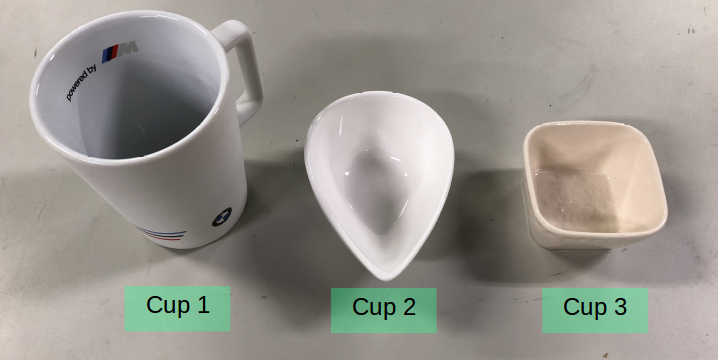
\includegraphics[width=0.8\linewidth]{fig/chp_pouring/Cups-v2.png}
	\caption{Containers used in experiment. Left container is Cup~1, middle is Cup~2, right is Cup~3.  
    % In the experience at Section~\ref{sec:exp0}, each cups had poured 20 times. In the experience of Method~1, each cups had poured 10 times. In the experience of Method~2, Cup~1 was not used, Cup~2 and Cup~3 were poured 15 times each in Section~\ref{sec:method-2-influence-of-surface-tension-on-method-2}, and 10 times each in Section~\ref{sec:Method2-expAll}.
    % TODO: Add right section ref
    }
	\label{fig:pour_cups}
\end{figure}

\begin{enumerate}
  \item \textbf{容器1：} 深さがあり底部が窄まった形状（最大容積 290\,ml）．
  \item \textbf{容器2：} 浅く広口の曲面形状（最大容積 120\,ml）．
  \item \textbf{容器3：} 角が丸い四角形の容器（最大容積 88\,ml）．
\end{enumerate}

手法1の実験では，注ぐ容器は内容量 1000\,ml の牛乳パックを，
注ぎ先容器は容器1--3のすべてをそれぞれ使用した．
手法2の実験では，注ぐ容器は容器1は平行グリッパでの安定把持が困難であったため
容器2および容器3のみを，注ぎ先容器には皿を使用した．


\subsubsection{液体および真値の取得}

実験で使用した液体は以下の通りである．
容積計算精度実験および手法1の実験ではミルクティー（液面検出しやすいため）を使用し，
あらかじめ実測した密度 $\rho = 1.0276\,\mathrm{g/cm^3}$ 
を用いて重量から体積に換算した．
手法2の実験では水道水（$\rho = 1.000\,\mathrm{g/cm^3}$）を使用した．

重量の計測には TANITA KD-320（3\,kg ロードセル）を用い，
測定範囲 0--300\,g では 0.1\,g，300--1500\,g では 0.5\,g の精度で
計測した．

評価指標としては，各試行における目標体積との誤差（注いだ体積 $-$ 目標体積）の
平均と標準偏差を用いる．

% ---------------------------------------------------------------------------
\subsection{容積計算精度の基礎評価}
\label{sec:pour_exp_volume_cal}
% ---------------------------------------------------------------------------

\subsubsection{実験方法}

提案手法の基礎となる容積計算の精度を評価するため，
各容器に対し，計量済みの液体を段階的に追加しながら，
液面検出に基づく容積計算を実施した．
容器1では 50\,ml 刻みで 50--250\,ml の5段階，5試行を実施した．
容器2では 25\,ml 刻み（25--100\,ml），容器3では 15\,ml 刻み（15--60\,ml）
の各4段階，各5試行の追加実験を実施した．
各試行で容器モデルを新規に構築し，液面検出を行った．

\subsubsection{実験結果}

% -------------------- IROS2019 Fig. result-VolumeCal --------------------
\begin{figure}[t]
	\centering
	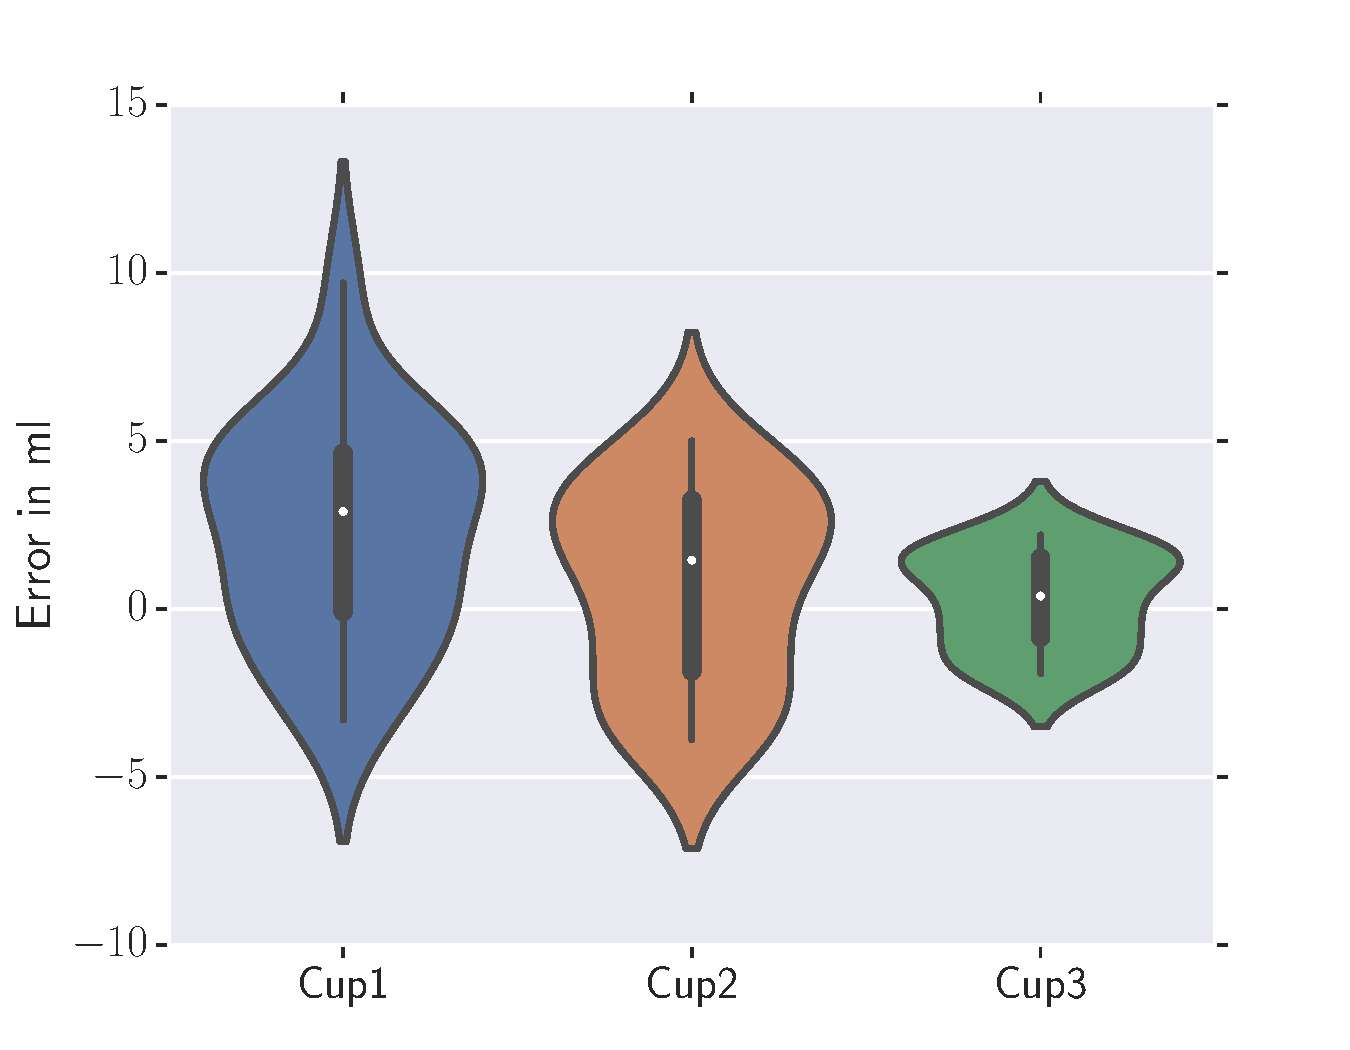
\includegraphics[width=0.8\linewidth]{fig/chp_pouring/VolumeCal.pdf}
	\caption{Results of volume-calculation accuracy. The horizontal axis is type of cup and it also represents the error distribution of each cup. The white dot is the median of errors. The thin black line is the 95\% confidence interval and the thick line is the interquartile range. }
	\label{fig:pour_result-VolumeCal}
\end{figure}
% ------------------------------------------------------------------------

\begin{table}[h]
	\vspace{3mm}
	\caption{The average (Avg.) and standard deviation (S.d.) of errors in volume calculation}
	\label{tab:pour_volume-calculation}
	\centering
	\begin{tabular}{cccc}
		\toprule
		& Cup 1 & Cup 2 & Cup 3 
		\\ \midrule
		Avg. (ml)            & 2.28  & 0.66  & 0.26  
		\\
		S.d. (ml) 			 & 3.29  & 2.94  & 1.44  
		\\ \bottomrule
	\end{tabular}
\end{table}

\subsubsection{考察}
本実験により，提案する体積計算手法の精度が容器形状に依存することが明らかとなった．
容器1では平均誤差2.28\,ml，標準偏差3.29\,mlと3種類中最大の誤差が生じたが，
これは底面が深く窄まった形状のためにカメラで底部まで十分な点群を取得できず，
モデル底面が不完全になることに起因する．
容器2では平均誤差0.66\,ml，標準偏差2.94\,mlであり，
浅く広口の曲面形状によって液面検出時のエッジに歪みが生じ，
RANSACで検出される液面高さが真値より過大評価される傾向が見られた．
一方，角が丸い四角形の容器3は点群取得・液面検出の双方で最も安定した結果を示し，
平均誤差0.26\,ml，標準偏差1.44\,mlという高い精度が得られた．
これらの3Dモデル誤差は，後述の注ぎ精度実験の結果を解釈するに使用する．

% ---------------------------------------------------------------------------
\subsection{手法1の注ぎ精度検証}
\label{sec:pour_exp_method1}
% ---------------------------------------------------------------------------

\subsubsection{実験方法}

手法1の注ぎ精度を評価するため，3種類の注ぎ先容器に対し
それぞれ2段階の目標体積を設定した（容器1：100, 200\,ml；
容器2：45, 90\,ml；容器3：30, 60\,ml）．
各条件で5回の注ぎを実施し，毎回注ぎ先容器のモデルを新規に構築した．

実験手順は以下の通りである：
\begin{enumerate}
  \item テーブル全体を撮影し，容器位置を認識する．
  \item 注ぎ先容器の内部点群を多視点から取得し，3Dモデルを構築する．
  \item 液面高さ--注いだ体積変換テーブルを作成し，容器のAABBを計算する．
  \item 左アームを，注ぎ動作に干渉せず容器内部を観測可能な位置に移動させる．
  \item 右アームで牛乳パックを把持し，注ぎ位置へ移動後，
        左アームのカメラで液面をリアルタイム検出しながら
        PD制御により注ぎを実行する．
  \item 停止条件到達後，戻し動作を実行する．
\end{enumerate}

\subsubsection{実験結果}

% -------------------- IROS2019 Fig. result-Method1 --------------------

\begin{figure}[t]
	\vspace{3mm}
	\centering
	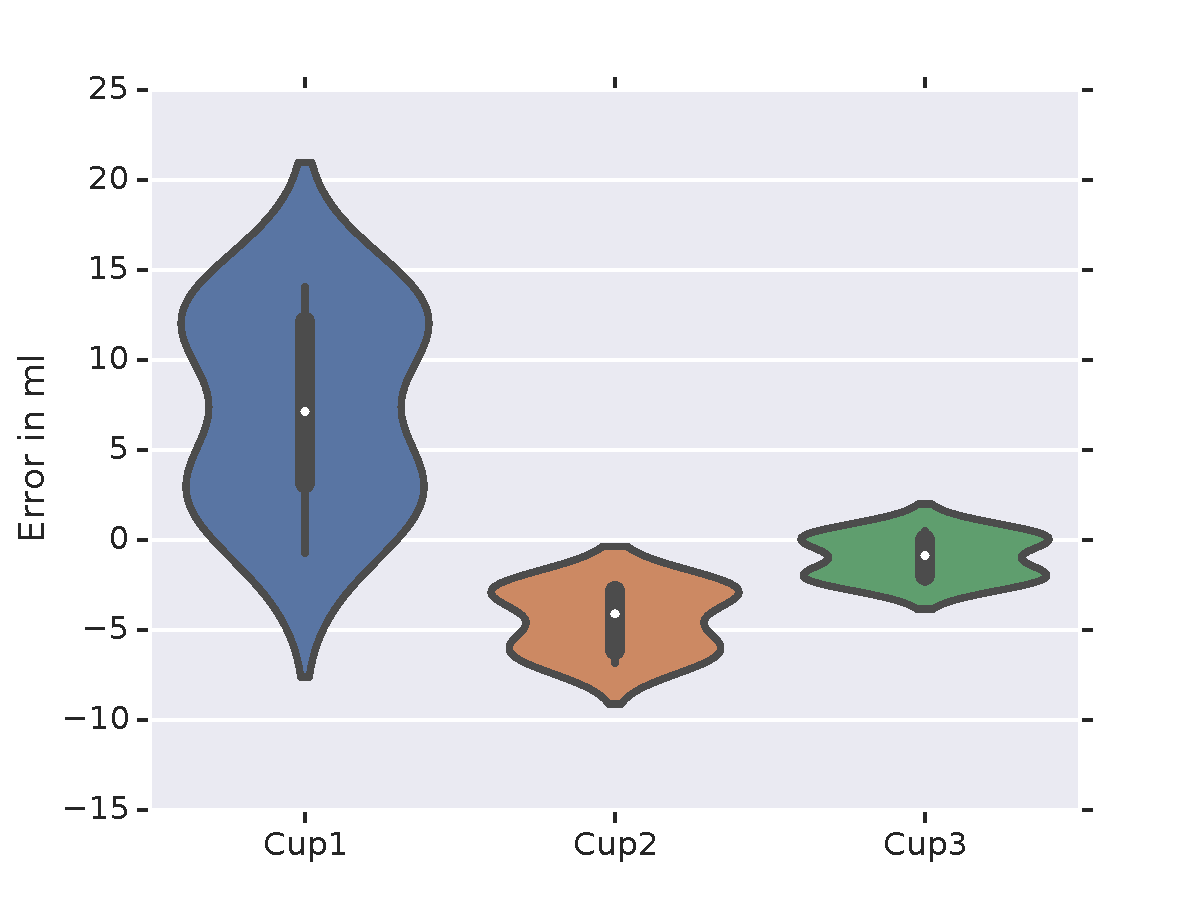
\includegraphics[width=0.8\linewidth]{fig/chp_pouring/Method1-Error.pdf}
	\caption{The accuracy of Method 1}
	\label{fig:pour_result-Method1}
\end{figure}
% ---------------------------------------------------------------------

\begin{table}[htbp]
  \centering
    \caption{The average (Avg.) and standard deviation (S.d.) of errors in  Method~1}
  \label{tab:pour_method1_error}
    \centering
    \begin{tabular}{cccc}
        \toprule
        & Cup 1 & Cup 2 & Cup 3 \\ \midrule
        Avg. (ml)            & 7.35  & -4.43  & -0.95  \\ 
        S.d. (ml) 			 & 5.45  & 1.79  & 1.16 
        \\ \bottomrule
    \end{tabular}
\end{table}

\subsubsection{考察}

手法1の注ぎ精度は容器形状によって大きく異なる結果となった．
容器1では平均誤差7.35\,ml，標準偏差5.45\,mlであり，
これは容積計算実験で確認された底部モデルの不完全性が直接的に影響したものである．
なお本実験では2種類の目標体積のみを設定したため，
図\ref{fig:pour_result-Method1}には二つのピークが現れており，
各ピークが各目標体積における注ぎ誤差の分布を表している．
容器2では平均誤差-4.43\,ml，標準偏差1.79\,mlと負の誤差が生じ，
注いだ液量が容器の容積に近づくにつれて液面と容器の縁が連結し，
液面エッジに歪みが生じて液面高さが高く評価され，
注ぎが早期に停止する現象が確認された．
\revise{容器3では平均誤差$-0.95$\,ml，標準偏差1.16\,mlと本実験中で最も小さい誤差を得た．ただし，この結果は内面と液面を安定に観測できる容器3と，本実験の低粘性・不透明液体に対するものであり，家庭調理全般に十分な性能を示すものではない．}
まとめると，手法1の誤差は容積計算精度実験と同程度の水準に収まっており，
システム全体の誤差は主として体積測定およびモデル精度に起因することが示唆される．


% ---------------------------------------------------------------------------
\subsection{手法2の注ぎ精度検証}
\label{sec:pour_exp_method2}
% ---------------------------------------------------------------------------

手法2では，まず表面張力が角度--注いだ体積関係の推測精度に及ぼす影響を評価し，
その評価を踏まえた上で手法2の注ぎ精度を検証した．

\subsubsection{表面張力の影響評価}
\label{sec:pour_exp_method2_st}

本実験では，\ref{sec:pour_angle_volume}節で提案した角度--注いだ体積関係の
推測アルゴリズムの精度を評価するとともに，表面張力が推測結果に与える
影響を調べた．

\textbf{実験方法：}
容器2および容器3を注ぐ容器とし，各々に初期液体体積を設定した．
容器2では 30, 60, 90\,ml，容器3では 22, 44, 66\,ml の3水準とした．
各初期液体体積に対し，容器を $0^\circ$ から注ぎ終わるまで $5^\circ$ 刻みで
$x$ 軸回りに回転させ，各角度における注いだ体積を秤で計測した．
各条件に対し5回の試行を実施し，毎回容器モデルを新規に取得した．
さらに，表面張力の影響を低減するため，容器の縁に洗剤を薄く塗布した条件
（表面張力なし条件）でも同様の計測を実施した．

\textbf{実験結果：}

% -------------------- IROS2019 Fig. method-exp1 (ST Cup2 and Cup3) --------------------
\begin{figure*}[t]
	\vspace{3mm}
	\centering
	\begin{subfigure}[t]{.45\textwidth}
		\centering
		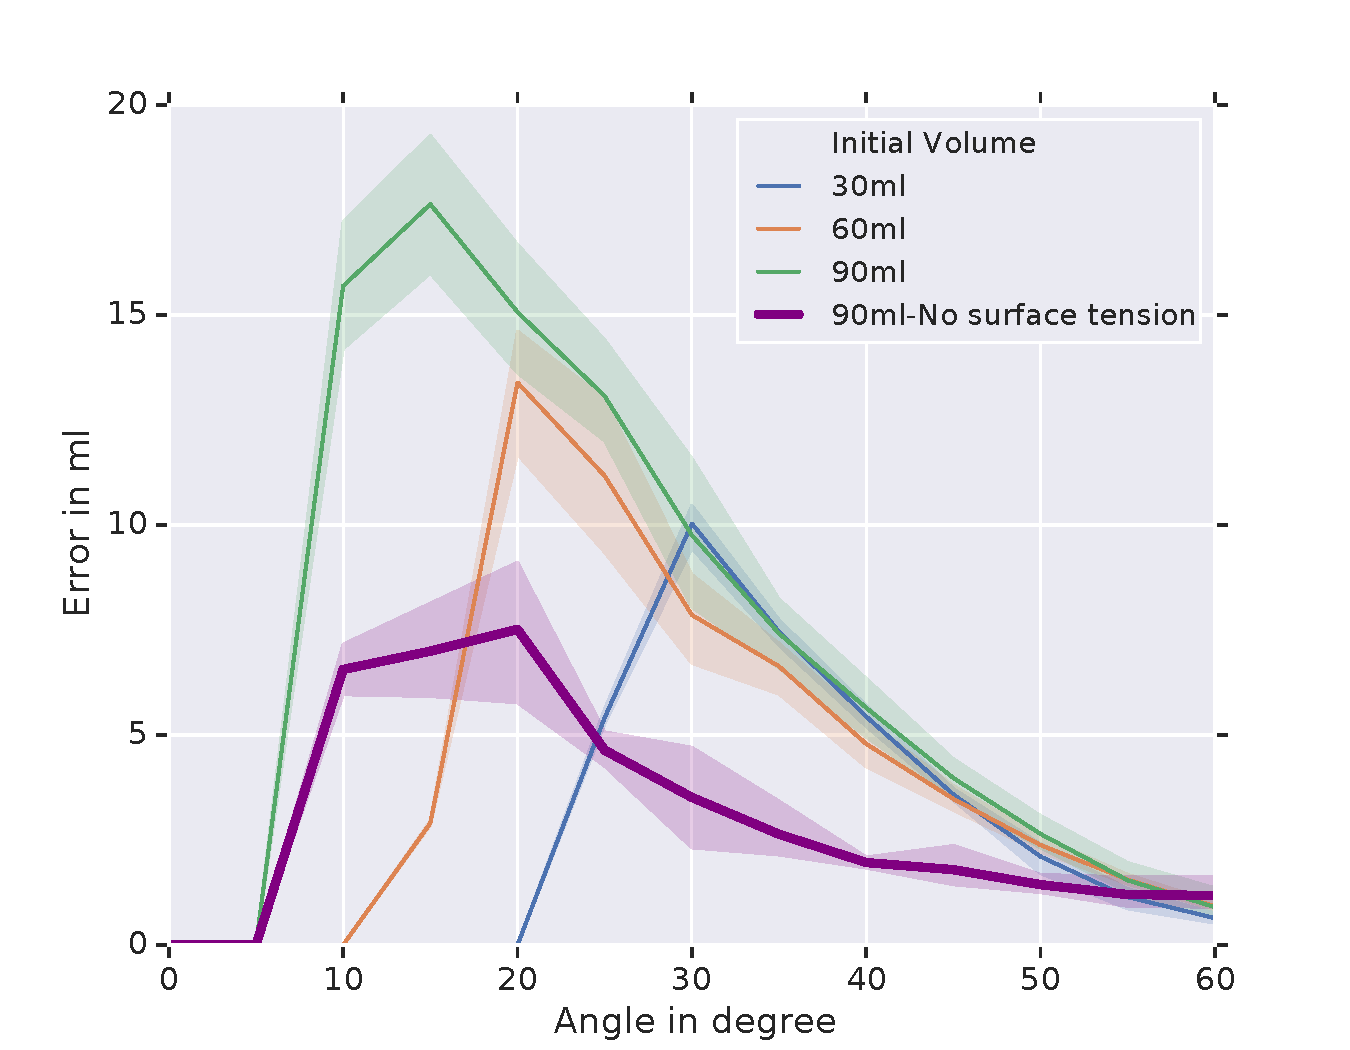
\includegraphics[width=1\textwidth]{fig/chp_pouring/Method2-ST-Cup2-Error.pdf}
		\caption{Errors with Cup~2.}
		\label{fig:pour_method-exp1.sub1}
	\end{subfigure}
	\hspace{1cm}
	\begin{subfigure}[t]{.45\textwidth}
		\centering
		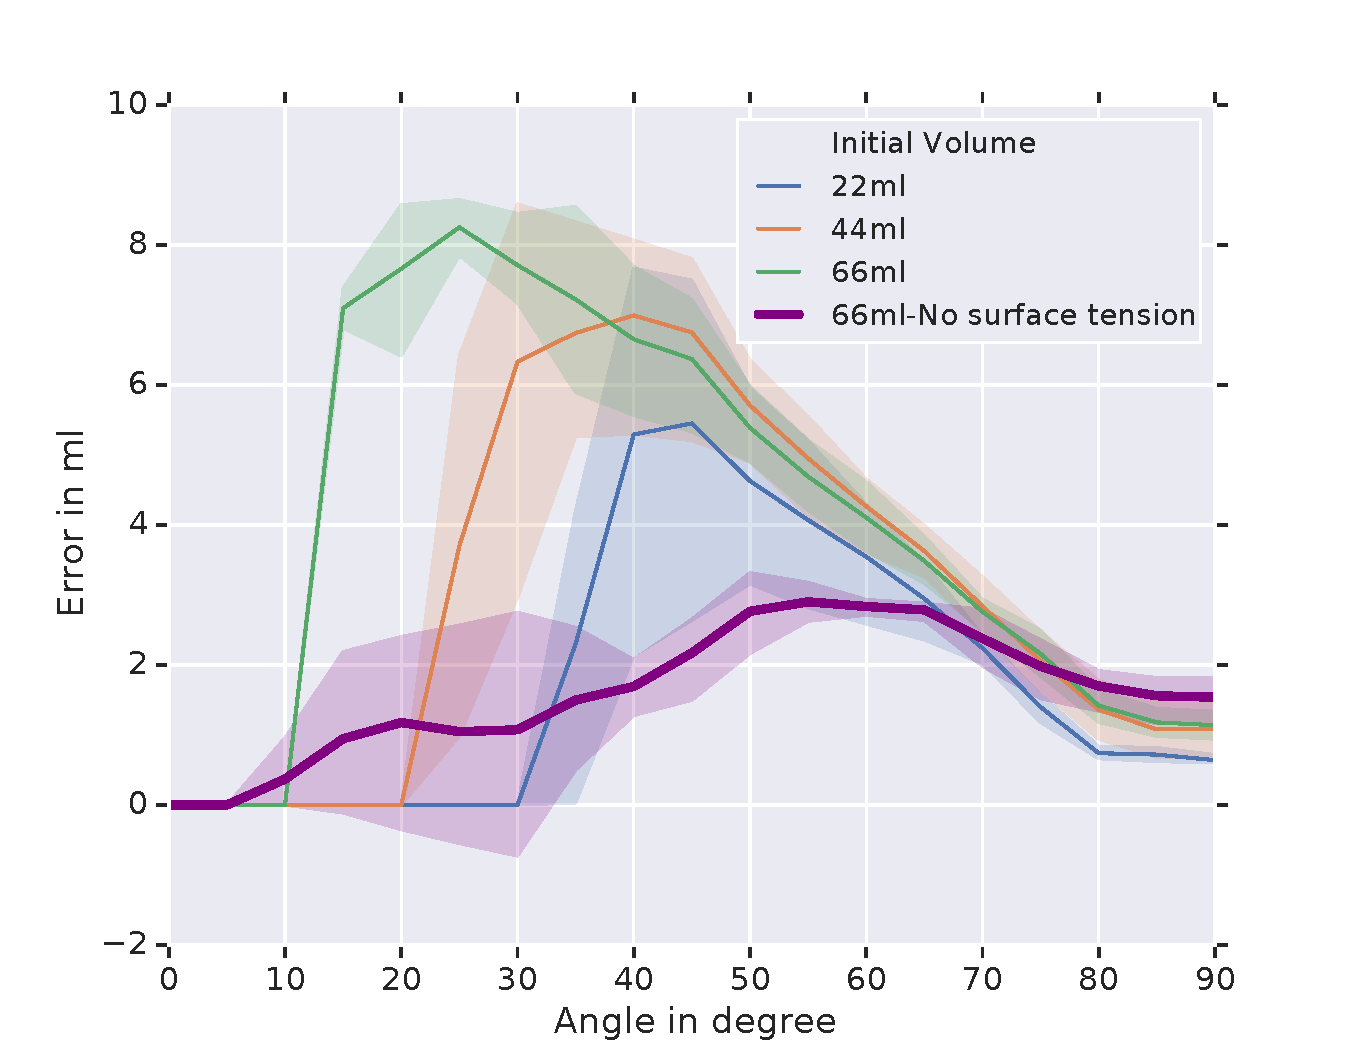
\includegraphics[width=1\textwidth]{fig/chp_pouring/Method2-ST-Cup3-Error.pdf}
		\caption{Errors with Cup~3}
		\label{fig:pour_method-exp1.sub2}
	\end{subfigure}
	\caption{Influence of Surface Tension on Method 2. In Figure \ref{fig:pour_method-exp1.sub1}, the blue, orange, and greeb lines show the results of Cup~2 with initial volumes of 30, 60, and 90\,ml, respectively. Cup~3 is 22, 44, and 66\,ml (Figure \ref{fig:pour_method-exp1.sub2}). The purple line shows the result with no surface tension and Cup~2 with an initial volume of 90\,ml.}
	\label{fig:pour_method-exp1}
\end{figure*}
% ------------------------------------------------------------------------------------

結果は図\ref{fig:pour_method-exp1}にしめした．
表面張力ありの条件では，注ぎ開始直後に $-10\,\mathrm{ml}$ から
$-5\,\mathrm{ml}$ の範囲に誤差が集中し，注ぎの進行とともに
誤差が減少する傾向が確認された．
一方，表面張力なし条件では，誤差の平均は 1.57\,ml，
標準偏差は 0.93\,ml まで大幅に低減した．

\textbf{考察：}
表面張力の有無による比較実験から，表面張力が注いだ体積積推定に与える影響が定量的に明らかとなった．
表面張力ありの条件では，注ぎ開始直後に$-10$\,mlから$-5$\,mlの範囲に誤差が集中し，
注ぎの進行とともに誤差が減少する傾向が認められた．
これは，注ぎ縁付近において液体と容器壁面の間に働く表面張力により液面が約3\,mm盛り上がるために，
実際に注がれた体積が推測値より小さくなることに起因する．
注ぎが進むにつれて液体と容器縁の接触面積が減少し，表面張力も徐々に弱まるため，誤差が収束する．
一方，容器の縁に洗剤を薄く塗布して表面張力を弱めた条件では，
容器2の最大誤差は約3\,ml，容器3の最大誤差は約7\,mlまで低減した．
ただし容器3では注ぎ開始直後に大量の水とともに洗剤が流れ出るため，
初期角度以降は表面張力低減効果が失われ，若干の誤差が残留した．
両条件の差から，表面張力の影響は容器3で最大約10\,ml程度と推定され，
容器2では約5\,mlとより小さいことが分かった．
これらの結果は，手法2において表面張力を考慮した補償の重要性を示している．


\subsubsection{手法2注ぎ精度の検証}
\label{sec:pour_exp_method2_all}

\textbf{実験方法：}  
表面張力の影響を含めた上で，手法2の総合的な注ぎ精度を評価した．  
実験には容器2および容器3を用いた．  
容器2では初期液体体積を100\,mlに，容器3では70\,mlに固定し，  
目標体積をそれぞれ0--95\,ml，0--65\,mlの範囲で5\,ml刻みに設定した．  
各目標体積につき4回の注ぎ試行を実施し，毎回新たに容器モデルを取得した．  
注ぎ動作は，\ref{sec:pour_angle_volume}節で求めた傾き角度と注いだ体積の関係に基づき，  
目標体積に対応する目標角度までP制御により容器を回転させる方法で行った．  
目標角度に到達後は残留液体の流出を待機し，戻し動作を実行した．

\textbf{実験結果：}  

% -------------------- IROS2019 Fig. Method2-ExpAll-Error --------------------
\begin{figure}[t]
	\centering
	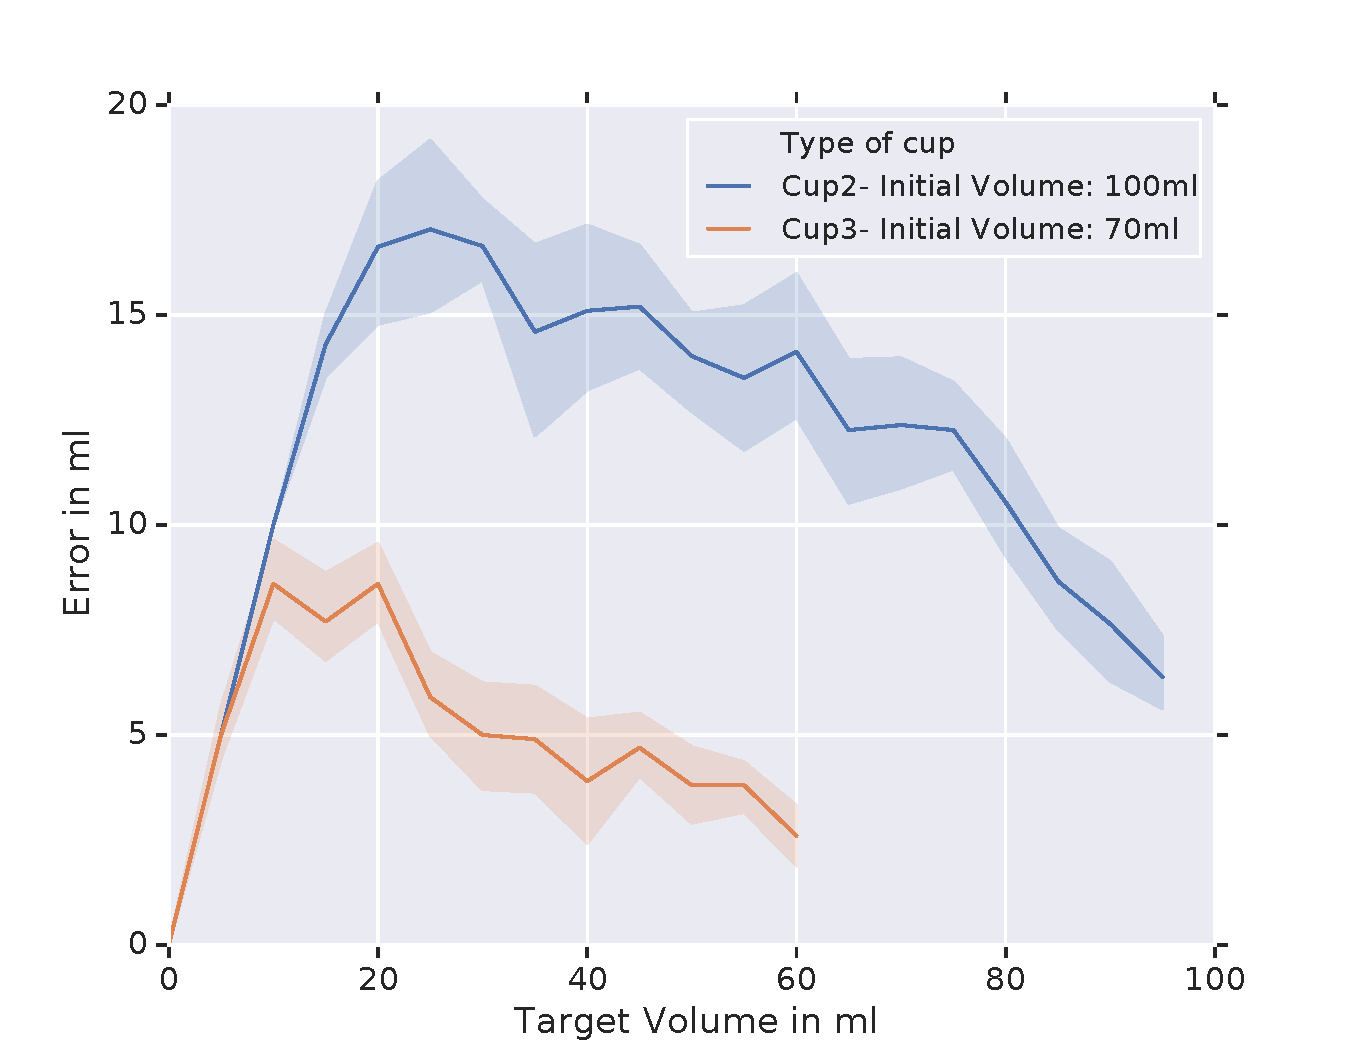
\includegraphics[width=0.9\linewidth]{fig/chp_pouring/Method2-ExpAll-Error.pdf}
	\caption{Errors of Method 2}
	\label{fig:pour_Method2-Cup2-Error}
\end{figure}
% ---------------------------------------------------------------------------

表\ref{tab:pour_method2_error}に誤差の平均と標準偏差を示す．

\begin{table}[h]
	\caption{The average (Avg.) and standard deviation (S.d.) of errors in  Method~2}
	\label{tab:pour_method2_error}
	\centering
	\begin{tabular}{ccc}
		\toprule 
		& Cup 2 & Cup 3 \\ 
		\midrule
		Avg. (ml)		& 11.88  & 4.96  \\ 
		S.D. (ml)		& 4.63  & 2.57 \\ 
		\bottomrule
	\end{tabular}
\end{table}
\textbf{考察：}
手法2の総合的な注ぎ精度は，容器2で平均誤差11.88\,ml，標準偏差4.63\,ml，
容器3で平均誤差4.96\,ml，標準偏差2.57\,mlとなり，手法1に比べて精度が劣ることが明らかとなった．
主な誤差要因は，注ぐ容器の内部点群が取得できないために外側点群からモデルを構築することによる
壁の厚さの影響と，表面張力の影響である．
容器2の最大誤差は約18\,mlに達しており，これは表面張力影響実験の結果と整合する．
また容器3では，表面張力の影響が最大約10\,mlと推定されることに加え，外側点群を用いることで
容器底部の厚さが容積計算に誤差をもたらしている．
手法2は注ぎ実行中の液面監視を必要とせず，カメラ配置の自由度が低い環境でも動作可能という
利点があるが，高精度が要求される場面では手法1の方が適していることが示された．

\subsection{両手法の比較考察}
\label{sec:pour_exp_discussion}

両手法の実験結果をまとめ，以下の比較考察が得られる．

% \begin{table}[t]
%   \centering
%   \caption{手法1 と 手法2 の比較}
%   \label{tab:pour_method_comparison}
%   \begin{tabular}{@{}p{0.28\textwidth}p{0.31\textwidth}p{0.31\textwidth}@{}}
%     \toprule
%     比較項目 & 手法1（注ぎ先容器基準） & 手法2（注ぐ容器基準） \\
%     \midrule
%     制御方式 & PD制御（注いだ体積積フィードバック） & P制御（角度追跡） \\
%     \midrule
%     精度（容器3） & 平均$-0.95\,\mathrm{ml}$ & 平均$4.96\,\mathrm{ml}$ \\
%     \midrule
%     主な誤差要因 & 液面検出精度 & 表面張力，容器壁の厚さ・変形 \\
%     \midrule
%     必要情報 & 注ぎ先容器内部形状 & 注ぐ容器形状＋初期液体体積 \\
%     \midrule
%     利点 & 高精度，注ぐ容器が未知でも可 &
%     注ぎ先容器の内部観測不要，実行中の液面監視不要 \\
%     \midrule
%     欠点 & 注いでいる間の液面観測必須 &
%     表面張力の影響が大きい，容器の個体差（壁の厚さ・変形）に敏感 \\
%     \bottomrule
%   \end{tabular}
% \end{table}

% TODO: 表格出去了。。。
\begin{table}[!t]
  \centering
  \caption{Comparison of Method 1 and Method 2}
  \label{tab:pour_method_comparison}
    \begingroup
  \footnotesize
  \setlength{\tabcolsep}{4pt}
  \renewcommand{\arraystretch}{0.95}
  \begin{tabularx}{.75\textwidth}{@{}p{0.28\textwidth}p{0.31\textwidth}p{0.31\textwidth}@{}}
    \toprule
    Item & Method 1 (target container based) & Method 2 (pouring container based) \\
    \midrule
    Control method & PD control (poured volume feedback) & P control (angle tracking) \\
    \midrule
    Accuracy (Cup 3) & Mean $-0.95\,\mathrm{ml}$ & Mean $4.96\,\mathrm{ml}$ \\
    \midrule
    Main error sources & Liquid level detection accuracy & Surface tension, container wall thickness \& deformation \\
    \midrule
    Required information & Internal shape of target container & Shape of pouring container and initial liquid volume \\
    \midrule
    Advantages & High accuracy; pouring container can be unknown &
    No need to observe interior of target container; no real-time liquid level monitoring required \\
    \midrule
    Disadvantages & Requires liquid level observation during pouring &
    Largely affected by surface tension; sensitive to container individual differences (wall thickness, deformation) \\
    \bottomrule
  \end{tabularx}
  \endgroup
\end{table}

\begin{enumerate}
  \item \textbf{精度：}  
  手法1（容器3における平均誤差 $-0.95\,\mathrm{ml}$，標準偏差 $1.16\,\mathrm{ml}$）は，手法2（同容器で平均誤差 $4.96\,\mathrm{ml}$，標準偏差 $2.57\,\mathrm{ml}$）より高い精度を達成した．  
  \revise{手法1の容器3での誤差は，事前学習や事前モデルを前提とする先行研究（約 $38\,\mathrm{ml}$ の誤差\cite{Related1}，約 $5\,\mathrm{ml}$ の誤差\cite{Related2}）と比較して小さい．ただし，容器1では平均誤差が7.35\,mlであり，精度は容器形状と観測条件に依存する．}
  \item \textbf{実装要件：}  
  手法1は注ぎ中の液面をリアルタイムに観測する必要があり，カメラ視野の確保や液面と容器縁の連結時への対策が不可欠である．  
  一方，手法2は事前の幾何計算のみで制御が完結するため，実装の制約が少ない．  
  \item \textbf{誤差要因の性質：}  
  手法1の誤差は主に液面検出精度（容器形状や液体の光学的性質に依存）に起因する．  
  手法2の誤差は主に表面張力および容器の壁の厚さ・変形（容器の物理的特性）に起因し，容器の個体差の影響を受けやすい．  
  \item \textbf{両手法の使い分け：}  
  \revise{高い定量性が要求される場合には，内面と液面を安定に観測できるなら手法1を優先する．一方，カメラ配置の自由度が低い環境や，大量の液体を注ぐため表面張力の相対的な影響が小さい場合には，手法2を選択できる．少量の調味料については，本実験の誤差を許容できるかをレシピ側の要求量と比較し，必要なら計量スプーンや秤を用いる．}
\end{enumerate}

\begin{revisionblock}
\subsection{家庭内の注ぎ作業としての評価}
家庭料理では小さじ1杯が約5\,mlであることを実用上の目安とすると，手法1の容器3では平均誤差の絶対値が1\,ml未満であり，観測しやすい容器へ比較的少量を注ぐ用途に可能性がある．
一方，手法1の容器1では平均7.35\,ml，手法2では容器2で11.88\,ml，容器3で4.96\,mlの誤差があり，小量の調味料では味への影響を無視できない．
手法2は液面を実時間観測しない利点があるため，水やだしなど比較的大きな量を移す用途に適するが，表面張力，容器壁厚，初期量の誤差を含む．

本実験で秤を用いたのは注いだ体積の真値を得る評価のためであり，提案制御への入力には用いていない．
したがって，「外部計測道具を用いない」とは制御時に補助計量器を用いないことを意味する．
現状は不透明な低粘性液体と三種類の開口容器に限られ，透明液体，粘性液体，泡，こぼれ，衛生・清掃，容器の再把持を含む家庭の一連作業は評価していない．
本章が示したのは，これらの条件下で，容器形状を直接利用して指定量に対応する制御目標を作れることである．
\end{revisionblock}


% ============================================================================
\section{本章のまとめ}
\label{sec:pour_summary}
% ============================================================================

\revise{本章では，事前登録していない容器の3D点群と，手法ごとに必要な液面または初期液体量を入力とし，注いだ体積または目標傾斜角度を出力して，指定量を注ぐ二つのタスク固有手法を示した．}
手法1は注ぎ先容器の液面高さを体積へ変換し，体積誤差に基づくPD制御を行う．
手法2は注ぐ容器の注ぎ縁と注ぐポイントを検出し，容器角度と注いだ体積の関係から目標角度を求めてP制御を行う．

これらの手法を実現した本章の成果は，以下の三点にまとめられる．
\begin{enumerate}
  \item \textbf{幾何学的な分析手法の応用：} 
    容器の3D点群モデルを基盤とし，
    (a) RANSACに基づくリアルタイム液面検出と注いだ体積への変換，
    (b) ConvexHullと複数姿勢投票による注ぎ縁・注ぐポイントの安定な検出，
    (c) 注ぎ角度--注いだ体積関係の計算
    の一連の幾何学的な分析手法を提案した．
  \item \textbf{分析結果に基づく動作制御の実装：}
    幾何学的な分析の結果を動作制御へ接続するため，
    手法1（注いだ体積フィードバックPD制御＋戻し動作）と
    手法2（目標角度追跡P制御＋残留液流出待機＋戻し動作）
    の2つの制御手法を設計・実装した．
  \item \textbf{実機実験による検証：}
    形状特性の異なる3種類の容器を用いた総計80回以上の注ぎ実験を通じて，
    手法1 では最小平均誤差 $-0.95\,\mathrm{ml}$（容器3），
    手法2 では平均誤差 $4.96\,\mathrm{ml}$（容器3）の精度を達成した．
    \revise{これにより，制御時に外部計量器を用いず，三種類の容器と設定した液体条件の範囲で定量注ぎが可能であることを示した．最小誤差は手法1・容器3の$-0.95\pm1.16$\,mlであったが，手法1・容器1では$7.35\pm5.45$\,ml，手法2・容器2では$11.88\pm4.63$\,mlであり，家庭用途への適否は容器，観測条件，およびレシピが許容する誤差に依存する．}
\end{enumerate}

本章の結果は，第\ref{ch:introduction}章\ref{tab:tasks}表に示した
検証作業のうち，「容器という環境を利用した流体操作」に対応するものであり，
\revise{容器という環境の幾何を液量または角度へ変換することで，直接把持できない液体に対する操作量を決定できることを示した．ただし，容器形状に依存する誤差，表面張力，粘性，観測困難な液面への対応は適用範囲外または今後の課題である．}
次章では，形状と環境の分析を中心とした本章から，包丁外力に抵抗する把持安定性の分析へ進む．食材形状，包丁軌道を同時に用い，力学的・環境的な分析から把持位置を決定する．

% 今後の課題として，ConcaveHull を用いた断面処理による凹型容器への拡張，
% 表面張力を考慮した角度--注いだ体積関係の補償モデルの導入，
% および液体の粘性が高い場合への対応が挙げられる．

	\chapter{タスク3：切断時の安定把持}
% ============================================================
\label{ch:holding}
% ============================================================

% ------------------------------------------------------------
\section{問題設定と本章の位置づけ}
\label{sec:holding_problem_and_role}
% ------------------------------------------------------------

\subsection{本章の位置づけ}
\label{subsec:holding_position}

\revise{本章は，第1章で整理した形状，力学，環境・道具という分析観点を，包丁による食材切断中の把持点選択へ適用した事例である．}

第3章で述べた3Dモデル取得基盤の上に，本章では食材表面上での把持点探索と包丁外力下での力学解析を積み上げ，双腕ロボットによる把持・切断動作の実行へと接続する．

本タスクは，包丁から食材に加わる力とトルクに抗して食材の意図しない移動を防ぐ{\nameholdingpointset}を，食材の三次元形状と包丁軌道を入力として解析的に算出する問題として定式化される．

\begin{revisionblock}
\subsection{想定する状況，目的および達成範囲}
本章は，家庭で食材を包丁により所定の位置で切断する際に，他方の手で食材を押さえて横滑りや回転を防ぐ操作を想定する．
ロボットには切断位置と包丁の往復軌道，指本数，食材種別に対応する破壊靭性・圧力分布・摩擦係数が既知または事前計測値として与えられ，食材表面の3D点群から安全かつ力学的に成立する接触位置を決定する．
実験では，まな板と安定な平面接触を持つ半切りのジャガイモおよび玉ねぎを対象とし，把持位置は切断前にオフラインで計算する．
食材・包丁の選択，切断軌道自体の自動生成，食材物性のオンライン推定，刃先周辺の人に対する安全監視，および切断後の搬送は対象外である．

達成目標は，包丁軌道全体にわたる切断力・モーメントと接触条件を用いて把持点を選び，切断中の食材移動を抑えて所定の切断を完了することである．
これは，「衝突せず指が届く」という幾何条件だけで把持点を選ぶ場合に比べ，実際の調理目的である食材の固定と切断完了へ評価を接続するものである．
\end{revisionblock}

\begin{revisionblock}
\subsection{幾何情報のみでは不十分な理由}
食材の3D形状からは，指先が接触可能か，指同士や包丁と衝突しないか，把持点が包丁平面から十分離れているかを判定できる．
しかし，同じ幾何配置でも，包丁の位置と速度により食材へ作用する力・モーメントの方向と大きさは時間的に変化する．
また，指先力が摩擦円錐内にあり，包丁Wrenchと釣り合い，特定の指だけに過大な力が集中しないことは，形状だけからは判断できない．
したがって，幾何情報は不適切な候補を除く第一段階として必要であるが，最終選択には切断力，摩擦，力・モーメントの釣合い，および包丁軌道全体にわたる時間変化を含む力学評価が必要である．
\end{revisionblock}


\subsection{提案手法の概要とアルゴリズムの流れ}
\label{subsec:holding_method_overview}

提案手法は，食材表面の離散点群モデル$\Omega$，包丁軌道$\mathbb{T}$，および指の本数$n$を入力とし，切断中の全時刻を通じて最も安定な把持を実現する{\nameholdingpointset}$\equholdingpointset[fin]$を出力するオフラインの探索アルゴリズムである．

アルゴリズムは包丁軌道の各時刻ステップにおいて，(1) 現在の包丁姿勢に基づく把持候補の生成，(2) 幾何フィルタによる{\namesearchspace}の削減，(3) 位置評価スコアの計算，(4) 力とトルクの推定，(5) {\namegraspforce}候補の生成と動的評価スコアの計算，を順次実行する．

全時刻の評価スコアを累積した後，最高スコアを得た{\nameholdingpointset}を最終出力とすることで，単一の包丁姿勢ではなく包丁軌道全体を考慮した把持計画を実現する点に本手法の特徴がある．


\subsection{点群情報の利用}
\label{subsec:holding_pointcloud}

本手法では，まずRGB-Dカメラをロボットアーム先端に搭載し，食材の周囲複数視点から点群を取得する．

取得した多視点点群は世界座標系へ変換・合成した後，移動最小二乗法（MLS）により平滑化し，さらに約150-200点へダウンサンプリングする．

このダウンサンプリング点数は，計算コストと評価スコアの関係を分析した上で経験的に決定した値であり，点数を増やしてもスコアはほとんど改善せず計算時間のみが増大することが確認されている（\ref{subsec:holding_exp_computation}節参照）．

また，力とトルクの推定に必要な切断接触面$\Omega_{\mathrm{c1}},\Omega_{\mathrm{c2}}$は，取得点群から直接得ることができないため，包丁切断平面への点群投影とDelaunay三角分割により計算的に生成する．

本手法で用いる記号の一覧を表\ref{tab:holding_symbol}にまとめる．

\begin{table}[t]
\caption{List of Symbols}
\centering
\label{tab:holding_symbol}
\begin{tabular}[t]{lll}
\hline
Symbol & Name & Description \\ \hline
$n$ & Number of fingers & Number of contact points\\
$\equfingerpoint[][i]$ & {\namefingerpointcapENG} & $xyz$ coordinates of the $i$-th contact point\\
$\equholdingpointset$ & {\nameholdingpointsetcapENG} & Set of $n$ contact points $\equfingerpoint$ \\
$\equsearchspace$ & {\namesearchspacecapENG} & Set of {\nameholdingpointsetENG}s $\equholdingpointset$ \\
$\bm{t}_\mathrm{k}$ & knife wrench & 6-D force and torque applied to the food \\
$\equfingerforce[i]$ & Finger tip force & 3-D Force vector of the $i$-th finger tip \\
$\equgraspforcevector$ & {\namegraspforcecapENG} & \begin{tabular}[c]{@{}l@{}}Vector of tip forces of $n$ fingers arranged\\  as a column, a $3n$-D vector\end{tabular} \\
$\Omega$ & & The surface shape of the food \\
$\Omega_{\mathrm{c1,2}}$ & & Contact surfaces (right part in Fig.\ref{fig:holding_method}) \\
% $\Omega_{\mathrm{g}}$ & & The surface part of the food used for holding 
$\Omega_{\mathrm{g}}$ & & 
\begin{tabular}[c]{@{}l@{}}The surface part of the food used for\\  holding\end{tabular}

\\
\hline
\end{tabular}
\end{table}

% ------------------------------------------------------------
\section{幾何情報による把持安定性の分析}
\label{sec:holding_analysis}
% ------------------------------------------------------------

\subsection{アルゴリズムの全体流れ}
\label{subsec:holding_algorithm_flow}

提案アルゴリズムの全体像をアルゴリズム \ref{algo:holding_global}に示す．

まず，食材表面$\Omega$の$K$個の離散点から$n$点を選ぶ全組合せとして全{\nameholdingpointset}$\equsearchspace_{\mathrm{all}}$を生成し，累積スコアを格納する辞書$\mathbb{S}$を初期化する．全{\nameholdingpointset}の要素数は組合せ数$\binom{K}{n}$となる．

メインループでは，包丁軌道$\mathbb{T}$の各時刻$(T,\bm{v})$に対し，現在の包丁姿勢$T$に基づいて食材表面を把持部$\Omega_{\mathrm{g}}$と切断接触面$\Omega_{\mathrm{c1}},\Omega_{\mathrm{c2}}$に分割する．その後，幾何フィルタ（\ref{subsec:holding_geometric_filter}節），位置評価スコア（\ref{subsec:holding_positional_score}節），力とトルクの推定（\ref{subsec:holding_knife_wrench}節），動的評価スコア（\ref{subsec:holding_dynamic_score}節）を順次計算し，各{\nameholdingpointset}のスコアを$\mathbb{S}$に加算する．各時刻で把持部$\Omega_{\mathrm{g}}$に含まれない{\nameholdingpointset}は無効とし，スコア$-\infty$を割り当てる．

全時刻の走査が完了した後，$\mathbb{S}$において最大値をとる{\nameholdingpointset}$\equholdingpointset[fin]$を最終出力とする．



\begin{algorithm}[H]
\caption{Full progress}\label{algo:holding_global}

\begin{algorithmic}[1]
\setlength{\baselineskip}{11pt}
\State $N$: the number of elements in $\mathbb{P}$
\State $\Omega$: A surface of food.
\State $\mathbb{T}$: Trajectory of knife, a sequence of pose $T$ and velocity $\bm v$
\State $\mathbb{S}$: Map for final evaluation score of a {\nameholdingpointsetENG} $P$. All scores initialize with 0.
% %% TAG: R1C1 ORG
% \State $\mathbb{P}_\mathrm{all}$: All possible {\nameholdingpointset} $P$ from $\Omega_{\mathrm{g}}$.
% %% TAG: R1C1
\State $\mathbb{P}_\mathrm{all}$: All possible {\nameholdingpointsetENG} $P$ from \fix[$\Omega$].

\State
\For{\textbf{all} $(T, \bm v) \in \mathbb{T}$}  \label{algoline:holding_global-knifepose-for-st}

    \State $\Omega_{\mathrm{c1}}, \Omega_{\mathrm{c2}}, \Omega_{\mathrm{g}}, \equsearchspace_\mathrm{init} \gets $\Call {PrepareData}{$\Omega$, $T$}  \label{algoline:holding_exp1-st}    \label{algoline:holding_global-PrepareData}
    \State $\equsearchspace \gets $\Call {FilterByGeoScore}{$\equsearchspace_\mathrm{init}$, $T$}

    \For{$P \in (\mathbb{P}_\mathrm{all} \setminus \equsearchspace)$  }  \label{algoline:holding_global-set-inf-score-st}
        \State $\mathbb{S}[\equholdingpointset] \gets -\infty$
    \EndFor  \label{algoline:holding_global-set-inf-score-ed}
  
    \State $\{S_\mathrm{pos, i}\} \gets$ \Call {CalPositionalScore}{$\equsearchspace$, $T$} 

    \State $\bm{t}_\mathrm{k} \gets $\Call {CalKnifeForce}{$\Omega_{\mathrm{c1}}$, $\Omega_{\mathrm{c2}}$, $T$, $\bm v$}  \label{algoline:holding_global-CalKnifeForce} \label{algoline:holding_global-filter-force-st}

    \State $\{S_\mathrm{force, i}\} \gets$ \Call {CalDynamicScore}{$\bm{t}_\mathrm{k}, \equsearchspace $, $\Omega_{\mathrm{g}}$} \label{algoline:holding_global-caldynamicscore}
  
    \For{$i\gets 1, N$} \label{algoline:holding_global-accumulate-forcescore-st}
        \State $ \mathbb{S}[\equholdingpointset[][i]] \gets \mathbb{S}[\equholdingpointset[][i]] + S_{\mathrm{pos}, i} + S_{\mathrm{force}, i}$
    \EndFor \label{algoline:holding_global-point-for-ed} \label{algoline:holding_global-filter-force-ed}  \label{algoline:holding_global-accumulate-forcescore-ed}
  
\EndFor  \label{algoline:holding_global-knifepose-for-ed}

\State $\equholdingpointset[fin] \gets P$ such that the value $\mathbb{S}[\equholdingpointset]$ is the maximum.

\end{algorithmic}
\end{algorithm}

\begin{figure}[ht]
    \centering
    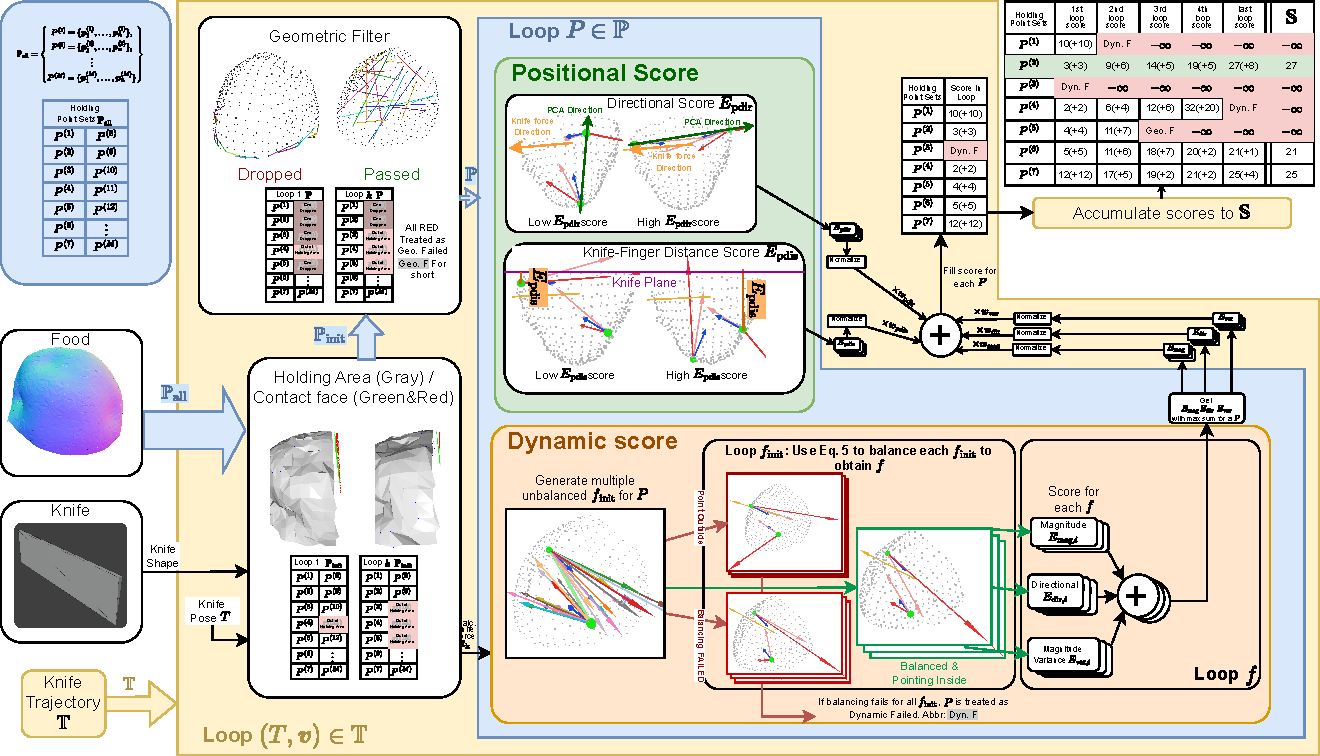
\includegraphics[width=1\linewidth]{fig/chp_holding/SICE2025_AlgoFlow.pdf}
    \caption{ Block diagram of the proposed searching method for the optimal {\nameholdingpointsetENG}. The process takes the food surface, knife mesh, and trajectory $\mathbb{T}$ as inputs. Inside the trajectory loop (yellow area), the search space is initialized and refined via a Geometric Filter. The remaining candidates in $\equsearchspace$ (blue area) are evaluated using Positional Scores (green block) and Dynamic Scores (orange block); the latter selects the best dynamic score of balanced {\namegraspforceENG} $\equgraspforce$ that can resist the knife wrench $\bm{t}_\mathrm{k}$. Finally, the normalized scores are accumulated in $\mathbb{S}$ to identify the final output. }
    \label{fig:holding_Algo1}
\end{figure}



\subsection{幾何フィルタによる{\namesearchspace}の削減}
\label{subsec:holding_geometric_filter}

全{\nameholdingpointset}$\equsearchspace_{\mathrm{all}}$の要素数は点群点数$K$に対して膨大となるため，後続の力学的評価に先立ち，低計算コストな幾何フィルタのみを用いたフィルタリングにより{\namesearchspace}を削減する（アルゴリズム \ref{algo:holding_filter_geo}）．

幾何スコア$S_{\mathrm{geo}}$は，「指同士の距離」「指と包丁の距離」「指の高さ」の3要素の重み付き和として定義される．

「指同士の距離」評価$E_{\mathrm{fin}}$は，二指が過度に接近して実質的に一指として機能することを防ぐために導入される．指間距離が閾値$b$を超えれば最大値1となり，それ以下の場合は指数関数的に減衰する設計とした．具体的には以下の式で定義される．
\begin{align*}
E_{\mathrm{fin}} &= \min_{\substack{i,j=1,\ldots,n\\ i\neq j}}(D(\|\equfingerpoint[][i] - \equfingerpoint[][j]\|))\\
D(x) &=
\begin{cases}
\displaystyle\ \frac{e^{ax/b} - 1}{e^a - 1} & (x \leq b)\\
\ 1 & (\text{otherwise})
\end{cases}
\end{align*}
ここで$a$は減衰の曲率を調整するパラメータ，$b$は指間距離の上限である．

「指と包丁の距離」評価$E_{\mathrm{knf}}$は，包丁の中心平面から各{\namefingerpoint}までの最短距離として定義され，切断動作中の手指と包丁の衝突を防止する役割を担う．
\begin{equation}
E_{\mathrm{knf}} = \min_{i=1,2,\cdots,n}(\mathrm{Dist}(\equfingerpoint[][i], \hat{\bm{n}}_{\mathrm{k}}, \bm{p}_{\mathrm{k}}))
\end{equation}
ここで$\hat{\bm{n}}_{\mathrm{k}}$は包丁平面の法線ベクトル，$\bm{p}_{\mathrm{k}}$は包丁の位置である．

「指の高さ」評価$E_{\mathrm{tbl}}$は，各指先の$z$座標の最小値として定義され，把持点がまな板に近すぎる候補を排除する．
\begin{equation}
E_{\mathrm{tbl}} = \min(p_{1z},\ldots,p_{nz})
\end{equation}

これら3つの評価値を$[0,1]$に正規化した後，重み$w_{\mathrm{fin}}, w_{\mathrm{knf}}, w_{\mathrm{tbl}}$により結合し，上位$\lfloor rN\rfloor$件の候補のみを後段へ出力する．
\begin{equation}
    S_{\mathrm{geo}} = w_{\mathrm{fin}} E_{\mathrm{fin}} + w_{\mathrm{knf}} E_{\mathrm{knf}} + w_{\mathrm{tbl}} E_{\mathrm{tbl}}
    \label{equ:holding_score_geo}
\end{equation}
本実験では出力比率$r=0.6$とした．なお，本フィルタでは指先が食材に接触した状態における拘束のみを考慮し，非接触状態から接触に至る指先の移動経路における衝突については考量しない．

\begin{algorithm}[!t]
\caption{Reduce the search space}
\label{algo:holding_filter_geo}
\begin{algorithmic}[1]
  \setlength{\baselineskip}{11pt}
  \Function{FilterByGeoScore}{$\mathbb{P}$, $T$}
  \State $N$: the number of elements in $\mathbb{P}$
  \State $P_1,\ldots,P_N$: each element of $\mathbb{P}$
  \State $w_\mathrm{fin}, w_\mathrm{knf}, w_\mathrm{tbl}$: weights
  \State \fix[$\mathbb{S}_\mathrm{geo}$: Local map for geometric scores, initialized empty]
  \State $r$: output ratio ($r\in(0, 1]$)
  \For{$i\gets 1, N$}
    \State $E_{\mathrm{fin}, i}\gets E_\mathrm{fin}$ for $P_i$
    \State $E_{\mathrm{knf}, i}\gets E_\mathrm{knf}$ for $P_i$
    \State $E_{\mathrm{tbl}, i}\gets E_\mathrm{tbl}$ for $P_i$
  \EndFor
  \State $\{E_{\mathrm{fin,}i}\}\gets$ \Call{Normalize}{$\{E_{\mathrm{fin,}i}\}$}
  \State $\{E_{\mathrm{knf,}i}\}\gets$ \Call{Normalize}{$\{E_{\mathrm{knf,}i}\}$}
  \State $\{E_{\mathrm{tbl,}i}\}\gets$ \Call{Normalize}{$\{E_{\mathrm{tbl,}i}\}$}
  \For{$i\gets 1, N$}
    \State $S_\mathrm{geo}\gets w_\mathrm{fin} E_{\mathrm{fin,}i} + w_\mathrm{knf} E_{\mathrm{knf,}i} + w_\mathrm{tbl} E_{\mathrm{tbl,}i}$ 
    \State \fix[$\mathbb{S}_\mathrm{geo}[P_i] \gets S_\mathrm{geo}$]
  \EndFor
  \State \fix[Sort $\mathbb{S}_\mathrm{geo}$ by values in descending order]
  \State \fix[$\mathbb{P}_\mathrm{out} \gets$ keys of the top $\lfloor rN\rfloor$ entries in $\mathbb{S}_\mathrm{geo}$]
  \State \fix[\textbf{return} $\mathbb{P}_\mathrm{out}$]
\EndFunction\\
\Function{Normalize}{$\{E_i\}$}  \label{algoline:holding_normalize-func}
\State $N$: the number of elements in $\{E_i\}$
\State $M\gets\max(E_1,\ldots,E_N)$
\State $m\gets\min(E_1,\ldots,E_N)$
\ForAll{$E\in\{E_i\}$}
 \State $E\gets (E - m) / (M - m)$
\EndFor
\State \textbf{return} $\{E_i\}$
\EndFunction  \label{algoline:holding_normalize-func-ed}
\end{algorithmic}
\end{algorithm}


\subsection{位置評価スコア}
\label{subsec:holding_positional_score}

本節は図\ref{fig:holding_Algo1}の中上部緑枠の「位置評価スコア」部分について述べる．

位置評価スコア$S_{\mathrm{pos}}$は，{\nameholdingpointset}の幾何的な配置が包丁から加わる力とトルクへの抵抗に適しているかを評価する指標であり，「方向」と「距離」の二要素から構成される（アルゴリズム \ref{algo:holding_score_pos}）．

「方向」評価$E_{\mathrm{pdir}}$は，{\nameholdingpointset}の主成分方向ベクトル$\mathrm{PCA}(\equholdingpointset)$と包丁平面法線$\hat{\bm{n}}_{\mathrm{k}}$の内積に基づいて定義される．
\begin{equation}
E_{\mathrm{pdir}} = 1 - |\mathrm{PCA}(\equholdingpointset) \cdot \hat{\bm{n}}_{\mathrm{k}}|
\end{equation}
主成分方向が包丁平面に平行であるほど高得点となり，これは多方向からの外力に対して有効に抵抗できる把持配置を優先する意図に基づく．

「距離」評価$E_{\mathrm{pdis}}$は，包丁中心平面から各把持点までの距離の最小値に負号を付して定義される．
\begin{equation}
E_{\mathrm{pdis}} = -\min(\mathrm{Dist}(\equholdingpointset, \hat{\bm{n}}_{\mathrm{k}}, \bm{p}_{\mathrm{k}}))
\end{equation}
包丁平面に近い位置で把持すればより小さな{\namefingerforce}でモーメントを打ち消せるという力学的直観を反映した設計である．

両評価値を$[0,1]$に正規化し，重み$w_{\mathrm{pdir}}, w_{\mathrm{pdis}}$により結合することで$S_{\mathrm{pos}}$を得る．
\begin{equation}
    S_{\mathrm{pos,}i} = w_{\mathrm{pdir}} E_{\mathrm{pdir,}i} + w_{\mathrm{pdis}} E_{\mathrm{pdis,}i}
    \label{equ:holding_score_pos_final}
\end{equation}

\begin{algorithm}[!t]
\caption{Calculate the positional score}
\label{algo:holding_score_pos}
\begin{algorithmic}[1]
\setlength{\baselineskip}{11pt}
\Function{CalPositionalScore}{$\mathbb{P}$, $T$}
    \State $N$: the number of elements in $\mathbb{P}$
    \State $P_1,\ldots,P_N$: each element of $\mathbb{P}$
    \State $w_\mathrm{pdir}, w_\mathrm{pdis}$: weights
    \For{$i\gets 1, N$}
        \State $E_{\mathrm{pdir,}i}\gets E_\mathrm{pdir}$ for $P_i$
        \State $E_{\mathrm{pdis,}i}\gets E_\mathrm{pdis}$ for $P_i$ \label{algoline:holding_CalDynamicScore-pos-score}
    \EndFor
    \State $\{E_{\mathrm{pdir,}i}\}\gets$ \Call{Normalize}{$\{E_{\mathrm{pdir,}i}\}$} \label{algoline:holding_score-pos-final-st}
    \State $\{E_{\mathrm{pdis,}i}\}\gets$ \Call{Normalize}{$\{E_{\mathrm{pdis,}i}\}$}
    \For{$i\gets 1, N$}
        \State $S_{\mathrm{pos},i} \gets w_\mathrm{pdir} E_{\mathrm{pdir},i} + w_\mathrm{pdis} E_{\mathrm{pdis},i}$
    \EndFor  \label{algoline:holding_score-pos-final-ed}

    \State \Return $\{S_{\mathrm{pos},i}\}$
\EndFunction
\end{algorithmic}
\end{algorithm}



\subsection{包丁が食材に与える力とトルクの推定}
\label{subsec:holding_knife_wrench}

包丁が食材に及ぼす力学的負荷$\bm{t}_{\mathrm{k}}\in\mathbb{R}^6$は，Muら\cite{method-cutting-fracture}の手法に基づき，食材の破壊靭性に起因する切断力と，包丁側面と食材接触面間に生じる摩擦力の二成分に分解して推定される．

\begin{figure*}[ht]
    \centering
    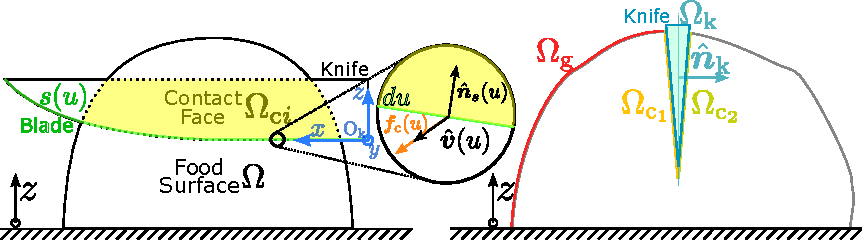
\includegraphics{fig/chp_holding/SICE2025-Method-fig1.pdf}
    \caption{Left: The zoomed-in part shows the calculation of the fracture force due to an infinitesimal element $du$ (in green text and line). Right: The crack generated by the knife creates two contact faces ($\Omega_\mathrm{c_{1}}$ and $\Omega_\mathrm{c_{2}}$). Also, searching only uses one side (the red curve) of the food model.}
    \label{fig:holding_method}
\end{figure*}

\subsubsection{切断力}

包丁の刃曲線を$s(u)$とパラメータ表示し，刃曲線上の位置$u$における包丁面法線ベクトルを$\hat{\bm{n}}_{s}(u)$，速度とその単位方向ベクトルをそれぞれ$\bm{v}(u)$，$\hat{\bm{v}}(u)$とする（図\ref{fig:holding_method}左）．食材の破壊靭性を$\kappa$とすると，位置$u$における微小切断力$\bm{f}_{\mathrm{c}}(u)$は次式で与えられる．
\begin{equation}
\bm{f}_{\mathrm{c}}(u) = -\kappa \left( \hat{\bm{v}}(u) \cdot \hat{\bm{n}}_{s}(u) \right) \hat{\bm{v}}(u)
\end{equation}
これを刃曲線全体にわたって積分することで，食材に作用する全切断力$\bm{f}_{\mathrm{c}}$が求められる．
\begin{equation}
\bm{f}_{\mathrm{c}} = \int \bm{f}_{\mathrm{c}}(u) \, \mathrm{d}u
\end{equation}
また，食材の重心位置$\bm{g}$を用いて，切断力が食材に与えるトルク$\bm{\tau}_{\mathrm{c}}$も併せて計算される．
\begin{equation}
\bm{\tau}_{\mathrm{c}} = \int \left( s(u) - \bm{g} \right) \times \bm{f}_{\mathrm{c}}(u) \, \mathrm{d}u
\end{equation}

\subsubsection{摩擦力}

第\ref{subsec:holding_position}節の仮定に基づき，切断接触面$\Omega_{\mathrm{c}j}$（$j = 1, 2$）に加わる圧力分布は一様（$P_{\mathrm{pres}}$）とする．包丁速度$\bm{v}$を各接触面へ射影した速度成分$\bm{v}_{\mathrm{c}j}$は，接触面の法線ベクトル$\hat{\bm{n}}_{\mathrm{c}j}$を用いて$\bm{v}_{\mathrm{c}j} = \bm{v} - (\bm{v} \cdot \hat{\bm{n}}_{\mathrm{c}j})\,\hat{\bm{n}}_{\mathrm{c}j}$と表される．包丁と食材間の摩擦係数を$\mu$とすると，クーロンの摩擦則に基づく摩擦力$\bm{f}_{\mathrm{fr}}$とトルク$\bm{\tau}_{\mathrm{fr}}$は次式で与えられる．
\begin{align*}
    & \bm{f}_{\mathrm{fr}} = \mu P_{\mathrm{pres}} \sum_{j=1}^2 \iint_{\Omega_{\mathrm{c}j}} \hat{\bm{v}}_{\mathrm{c}j} \, \mathrm{d}S,\\
    & \bm{\tau}_{\mathrm{fr}} = \mu P_{\mathrm{pres}} \sum_{j=1}^2 \iint_{\bm{x} \in \Omega_{\mathrm{c}j}} (\bm{x} - \bm{g}) \times \hat {\bm{v}}_{\mathrm{c}j}\, \mathrm{d}S.
\end{align*}
ここで$S$は接触面$\Omega_{\mathrm{c}j}$の微小面積要素，$\bm{x}$はその中心位置を表す．

\subsubsection{力とトルクの合成}

以上の切断力と摩擦力を6次元ベクトルとして合成した
\begin{equation}
\bm{t}_{\mathrm{k}} = \left[ \left( \bm{f}_{\mathrm{fr}} + \bm{f}_{\mathrm{c}} \right)^{\mathrm{T}}, \left( \bm{\tau}_{\mathrm{fr}} + \bm{\tau}_{\mathrm{c}} \right)^{\mathrm{T}} \right]^{\mathrm{T}}
\label{equ:holding_knife_wrench}
\end{equation}
を，包丁が食材に与える力とトルクとして定義する．


\subsection{{\namegraspforce}候補の効率的生成}
\label{subsec:holding_force_generation}

{\nameholdingpointset}$\equholdingpointset$が定まったとしても，包丁から食材に加わる力とトルク$\bm{t}_{\mathrm{k}}$と釣り合うべき{\namegraspforce}$\equgraspforce\in\mathbb{R}^{3n}$には，把持行列$G$の零空間に起因する無限の冗長性が存在する．

まず，{\namegraspforce}とその合力の関係を定式化する．本研究では指先と食材の接触を点接触と仮定し，指先におけるトルクを無視して各{\namefingerforce}$\equfingerforce[i]$（$i = 1,\ldots, n$）のみを考える．これらを$3n$次元ベクトル$\equgraspforce = [\equfingerforce[1]^{\mathrm{T}},\ldots, \equfingerforce[n]^{\mathrm{T}}]^{\mathrm{T}}$に並べたものを{\namegraspforce}と定義する．{\namegraspforce}$\equgraspforce$が食材に与えた合力を$\bm{t}_{\mathrm{h}} = [\bm{f}_{\mathrm{h}}^{\mathrm{T}}, \bm{\tau}_{\mathrm{h}}^{\mathrm{T}}]^{\mathrm{T}}$とすると，これは包丁の力とトルクと釣り合う必要があり，$\bm{t}_{\mathrm{h}} = -\bm{t}_{\mathrm{k}}$を満たす．

ここで，食材がまな板と安定な平面接触を有し，その運動が$xy$平面内の並進と$z$軸まわりの回転に限定されるという仮定のもとでは，$z$軸方向の力および$x$,$y$軸まわりのトルクはまな板によって相殺される．したがって，必要な合力 $\bm{t}_{\mathrm{h}}$としては力の$x$,$y$成分とトルクの$z$成分のみを考慮すればよく，これを$[f_{\mathrm{h}x}, f_{\mathrm{h}y}, \tau_{\mathrm{h}z}]$と抽出する．

{\namegraspforce}$\equgraspforce$と合力 $\bm{t}_{\mathrm{h}}$の関係は，把持行列$G$を用いて$\bm{t}_{\mathrm{h}} = G \equgraspforce$と表される．把持行列$G$は次の式で定義される$6 \times 3n$行列である．
\begin{equation}
    G = \begin{bmatrix}I_3 & \cdots & I_3 \\ R_1 & \cdots & R_n \end{bmatrix}
    \label{equ:holding_grasp_matrix}
\end{equation}
ここで$I_{3}$は$3 \times 3$の単位行列，$R_{i}$は$\equfingerpoint[][i] - \bm{g}$から構成される歪対称行列であり，$R_i \equfingerforce[i] = (\equfingerpoint[][i] - \bm{g}) \times \equfingerforce[i]$を満たす．実際には，抽出された3成分$[f_{\mathrm{h}x}, f_{\mathrm{h}y}, \tau_{\mathrm{h}z}]$に対応させるため，$G$の3,4,5行目を除いた行列を用いる．この式を$\equgraspforce$について解くと次の式が得られる．
\begin{equation}
    \equgraspforce = G^+ \bm{t}_{\mathrm{h}} + [I_{3n}-G^+ G]\,\bm{k}
    \label{equ:holding_force_balance}
\end{equation}
ここで$G^+$は$G$の擬似逆行列，$\bm{k}$は任意の$3n$次元ベクトルである．$\bm{k}$の選び方により無数の{\namegraspforce}が得られることから，力の冗長性が生じる．

この冗長性に対処するため，本手法ではまず多数の{\namegraspforce}候補を生成し，その中から最適なものを選択する戦略をとる．最も単純な生成法は，式(\ref{equ:holding_force_balance})の任意ベクトル$\bm{k}$に乱数を割り当てる方法である．しかし，このアプローチでは生成された{\namefingerforce}の多くが摩擦円錐の外側を向く，すなわち物理的に妥当でない解となり，生成効率が極めて低い．

そこで提案手法では，二段階の生成方法を提案する．
\begin{enumerate}
    \item 第一段階では，各{\namefingerforce}の方向を摩擦円錐内に限定した初期力$\equgraspforcevector[init]$をランダムに生成する．
    \item 第二段階では，以下の補正式により$\equgraspforcevector[init]$と包丁の力とトルクとの釣り合わない分を補正し，釣り合える{\namegraspforce}$\equgraspforce$を得る．
    \begin{align*}
        \bm{t} &= (-\bm{t}_{\mathrm{k}}) - G \equgraspforcevector[init] \\
        \equgraspforce &= \equgraspforcevector[init] - G^{+}\bm{t}
    \end{align*}
\end{enumerate}

この提案手法により，摩擦円錐内に収まる妥当な{\namegraspforce}候補を，ランダム$\bm{k}$法と比較して平均約7.7倍の効率で生成できることが実験的に確認されている（\ref{subsec:holding_exp_force_generation}節参照）．それでも妥当な{\namefingerforce}が一つも生成できない{\nameholdingpointset}については，無効候補としてスコア$-\infty$を割り当てる．


\subsection{動的評価スコア}
\label{subsec:holding_dynamic_score}

動的評価スコア$S_{\mathrm{dyn}}$は，前節で生成された{\namegraspforce}候補群の中から，力量の大きさ・方向・分散の三基準で最も安定と判定される力を{\nameholdingpointset}ごとに選出し，{\namesearchspace}全体で正規化した評価値である（アルゴリズム \ref{algo:holding_filter_force}）．

動的評価は二段階で構成される．第一段階（ローカル評価）では，単一の{\nameholdingpointset}$\equholdingpointset$に対して生成された全{\namegraspforce}候補を対象に，三基準の重み付きスコアを計算し，最高スコアに対応する力候補のスコアを返す．

力量の大きさ評価$e_{\mathrm{mag}}$は，全{\namefingerforce}のノルム和の負値として定義され，小さな力で把持可能な候補ほど高得点となる．
\begin{equation}
e_{\mathrm{mag}} = - \sum_{i=1}^n \|\equfingerforce[i]\|
\label{equ:holding_emag}
\end{equation}

方向評価$e_{\mathrm{dir}}$は，各{\namefingerforce}ベクトルと接触点における食材表面法線との内積和として定義される．{\namefingerforce}が表面法線方向に近いほど滑りにくいため，この値が大きい候補が優先される．
\begin{equation}
e_{\mathrm{dir}} = \sum_{i=1}^n \hat{\bm{n}}_{\Omega} (\equfingerpoint[][i]) \cdot \hat{\equfingerforce[i]}
\label{equ:holding_edir}
\end{equation}
ここで$\hat{\bm{n}}_{\Omega} (\equfingerpoint[][i])$は食材表面$\Omega$の位置$\equfingerpoint[][i]$における単位法線ベクトルである．

分散評価$e_{\mathrm{var}}$は，各{\namefingerforce}の大きさの分散の負値として定義され，特定の指に力が集中することを避け，全指への均等な負荷分散を促す役割を担う．
\begin{equation}
e_{\mathrm{var}} = - \mathrm{Var}(\|\equfingerforce[1]\|, \|\equfingerforce[2]\|, \dots, \|\equfingerforce[n]\|)
\label{equ:holding_evar}
\end{equation}

これらの三評価値は，一つの{\nameholdingpointset}$\equholdingpointset$に対して生成された全{\namegraspforce}候補間で$[0,1]$にローカル正規化され，重み付き和としてローカルスコア$S$が算出される．
\begin{equation}
    S = w_{\mathrm{mag}} \tilde{e}_{\mathrm{mag,}i} + w_{\mathrm{dir}} \tilde{e}_{\mathrm{dir,}i} + w_{\mathrm{var}} \tilde{e}_{\mathrm{var,}i}
    \label{equ:holding_force_local_score}
\end{equation}
これらのローカルスコア$S$と対応する生素点$\{e_{\mathrm{mag}}, e_{\mathrm{dir}}, e_{\mathrm{var}}\}$がリスト$L$に格納され（アルゴリズム\ref{algo:holding_filter_force}の\ref{algo:holding_force-local-norm-score-st}行），最高の$S$に対応する生素点がローカル段階の出力として返される（アルゴリズム\ref{algo:holding_filter_force}の\ref{algo:holding_force-local-norm-score-ed}行）．

第二段階（グローバル評価）では，ローカル段階で選出された各{\nameholdingpointset}の生素点（$E_{\mathrm{mag}}$, $E_{\mathrm{dir}}$, $E_{\mathrm{var}}$）を{\namesearchspace}$\equsearchspace$全体で$[0,1]$に正規化し，重み付き和として$S_{\mathrm{dyn}}$を算出する．
\begin{equation}
S_{\mathrm{dyn},i} = w_{\mathrm{mag}} \tilde{E}_{\mathrm{mag,}i} + w_{\mathrm{dir}} \tilde{E}_{\mathrm{dir,}i} + w_{\mathrm{var}} \tilde{E}_{\mathrm{var,}i}
\label{equ:holding_force_final_score}
\end{equation}
本実験では，重みを$w_{\mathrm{dir}}=2,\ w_{\mathrm{mag}}=2,\ w_{\mathrm{var}}=1$と設定した．

\begin{algorithm}[!t]
\caption{Algo of the holding score calculation}
\label{algo:holding_filter_force}
\begin{algorithmic}[1]
\setlength{\baselineskip}{11pt}
\Function{CalDynamicScore}{$\bm{t}_\mathrm{k}$, $\equsearchspace$, $\Omega_{\mathrm{g}}$}
    \State $E_{\mathrm{mag,}i} , E_{\mathrm{dir,}i} , E_{\mathrm{var,}i}$: The each part of dynamic score for a $P$

    \For {$i\gets 1, N$}
        \State \fix[$E_{\mathrm{mag,}i} , E_{\mathrm{dir,}i} , E_{\mathrm{var,}i}$ ]
        \State $\quad \gets$ \Call {CalDynamicScoreEach}{$\bm{t}_\mathrm{k}, \equholdingpointset[i] $, $\Omega_{\mathrm{g}}$}
    \EndFor
    
    \State \fix[$\{\tilde{E}_{\mathrm{mag,}i}\}\gets$ \Call{Normalize}{$\{E_{\mathrm{mag,}i}\}$} \label{algo:holding_force-global-norm-score-st} ]
    \State \fix[$\{\tilde{E}_{\mathrm{dir,}i}\}\gets$ \Call{Normalize}{$\{E_{\mathrm{dir,}i}\}$}]
    \State \fix[$\{\tilde{E}_{\mathrm{var,}i}\}\gets$ \Call{Normalize}{$\{E_{\mathrm{var,}i}\}$}] \label{algo:holding_force-global-norm-score-ed}
    
    \For{$i\gets 1, N$}
        \State \fix[$S_{\mathrm{dyn},i} \gets w_\mathrm{mag} \tilde{E}_{\mathrm{mag,}i} + w_\mathrm{dir} \tilde{E}_{\mathrm{dir,}i} + w_\mathrm{var} \tilde{E}_{\mathrm{var,}i}$ ]
    \EndFor
    
    \State \fix[\Return $\{S_{\mathrm{dyn,}i}\}$ \label{algoline:holding_CalDynamicScore-all}]
\EndFunction

\State 

\Function{CalDynamicScoreEach}{$\bm{t}_\mathrm{k}$, $\equholdingpointset$, $\Omega_{\mathrm{g}}$}
    \State \fix[$e_\mathrm{mag},e_\mathrm{dir},e_\mathrm{var}$: Local dynamic score of a generated {\namegraspforceENG}.]
    \State $L$: an empty list
    \State $\fix[Q]$: the number of \fix[\namegraspforceENG] to generate
    \State $[\equgraspforce_\mathrm{1}, \equgraspforce_\mathrm{2}, \dots \equgraspforce_{\fix[Q]}]\gets $\Call {\fix[Generate\namegraspforcetitleENG]}{$\bm{t}_\mathrm{k}, \equholdingpointset$}  
    \label{algoline:holding_CalDynamicScore-GenerateFingerForce-1} \label{algoline:holding_CalDynamicScore-GenerateFingerForce-2} \label{algoline:holding_exp1-ed}
    
    \For{$i\gets 1, \fix[Q]$}
        \State \fix[$e_{\mathrm{mag,}i}\gets $ Calculate $e_{\mathrm{mag}}$ given $\bm{t}_\mathrm{k}, P, \bm{f}_i$ \label{algoline:holding_CalDynamicScore-force-score-st}]
        \State \fix[$e_{\mathrm{dir,}i}\gets $ Calculate $e_{\mathrm{dir}}$ given $\bm{t}_\mathrm{k}, P, \bm{f}_i$ ]
        \State \fix[$e_{\mathrm{var,}i}\gets $ Calculate $e_{\mathrm{var}}$ given $\bm{t}_\mathrm{k}, P, \bm{f}_i$ \label{algoline:holding_CalDynamicScore-force-score-ed}]
    \EndFor \label{algoline:holding_CalDynamicScore-force-score-loop-ed}

    \State \fix[$\{\tilde{e}_{\mathrm{mag,}i}\}\gets$ \Call{Normalize}{$\{e_{\mathrm{mag,}i}\}$} \label{algo:holding_force-local-norm-score-st}]
    \State \fix[$\{\tilde{e}_{\mathrm{dir,}i}\}\gets$ \Call{Normalize}{$\{e_{\mathrm{dir,}i}\}$}]
    \State \fix[$\{\tilde{e}_{\mathrm{var,}i}\}\gets$ \Call{Normalize}{$\{e_{\mathrm{var,}i}\}$} \label{algo:holding_force-local-norm-score-ed}]

    \For{$i\gets 1, M$} \label{algoline:holding_CalDynamicScoreEach-finalscore-st}
        \State \fix[$S_{\mathrm{}}\gets w_\mathrm{mag} \tilde{e}_{\mathrm{mag,}i} + w_\mathrm{dir} \tilde{e}_{\mathrm{dir,}i} + w_\mathrm{var} \tilde{e}_{\mathrm{var,}i}$ ]
        \State \fix[Append $\{S, \{e_{\mathrm{mag,}i},e_{\mathrm{dir,}i},e_{\mathrm{var,}i}\}\}$ to $L$]
    \EndFor

    \State \fix[Find element in $L$ with maximum $S$]
    \State \fix[\Return the raw values $\{e_{\mathrm{mag,}i},e_{\mathrm{dir,}i},e_{\mathrm{var,}i}\}$ of that element.] \label{algoline:holding_sub-return}
    
\EndFunction
\end{algorithmic}
\end{algorithm}


% ------------------------------------------------------------
\section{安定把持ための動作計画・制御}
\label{sec:holding_control}
% ------------------------------------------------------------

% TODO: 重写
\subsection{分析結果から動作指令への変換}
\label{subsec:holding_execution}

前節までの分析により計算された{\nameholdingpointset}$\equholdingpointset[fin]=\{\equfingerpoint[][1],\equfingerpoint[][2]\}$は，食材表面上の目標接触位置を与えるが，それ自体はロボットの動作指令ではない．本節では，この分析結果を双腕ロボットの関節指令へ変換し，把持から切断に至る一連の動作として実行する方法を述べる．

動作制御の流れは，以下の3段階からなる．
\begin{enumerate}
    \item 把持点$\equfingerpoint[][1],\equfingerpoint[][2]$を目標値とし，左腕指ハンドの逆運動学により各指関節角を計算する．
    \item 指先を食材表面へ接触させ，把持を完了する．
    \item 右腕に固定された包丁を，事前計画された切断軌道に沿って動作させる．
\end{enumerate}
このうち，(1)および(2)は分析結果を直接反映する実行段階であり，(3)は分析フェーズにおいて力学的評価の前提条件として参照された包丁軌道そのものを実機上で再現する段階である．


\subsection{把持点への手指配置}
\label{subsec:holding_finger_placement}

実験プラットフォームの詳細は第3章にて述べた通りであり，左腕には食材形状への適応性を重視した3軸2指サーボハンド（図\ref{fig:system:finger-hand}）を，右腕には包丁を固定するための平行グリッパを装着した．

指ハンドの各指はz-y-y-tipの関節構成をとり，FUTABA RS405CBサーボ（最大トルク48.0\,$\mathrm{kgf \cdot cm}$，角度分解能0.1\,deg）により駆動される．{\namefingerpoint}$\equfingerpoint[][i]$から関節角$\bm{q}_i$への変換には，指関節のみのヤコビアン逆運動学を用いた．
\begin{equation}
\Delta\bm{q}_i = J_i^{+}(\bm{q}_i)\, \Delta\equfingerpoint[][i]
\end{equation}
ここで$J_i^{+}$は第$i$指のヤコビアン行列$J_i$の擬似逆行列であり，$\Delta\equfingerpoint[][i]$は現在の{\namefingerpoint}から目標位置$\equfingerpoint[][i]$への変位である．

{\namefingerpoint}制御にはPID制御を用いたが，サーボの駆動電流に設定された不感帯（最大電流の13\%）に起因して，{\namefingerpoint}に最大約1cmの誤差が生じうる点が実装上の制約として残されている．この位置決め誤差は，\ref{subsec:holding_exp_comparison}節で述べる把持安定性評価における外れ値の一因ともなった．


\subsection{包丁軌道の設計と実行}
\label{subsec:holding_knife_trajectory}

切断軌道の設計は，分析フェーズにおける力とトルクの推定（\ref{subsec:holding_knife_wrench}節）と表裏一体の関係にある．包丁の位置姿勢$T$と速度$\bm{v}$の系列$\mathbb{T}$は，把持点探索の入力であると同時に，動作制御フェーズでは右腕が実際に追跡すべき目標軌道となる．

本研究では，Zhouら\cite{Cutting-Slice-1,Cutting-Slice-2}により報告された「包丁を真下に押し込むよりも前後にスライドさせながら切る方が切断に要する力が少なくて済む」という知見に基づき，往復スライス軌道を採用した．軌道は，まな板面に対して25度の角度で下降する二段階構成とした．

%%% TODO: 重新整理这段的意思．
\begin{description}
    \item[前進下降] 包丁を前方かつ下方へ，まな板面から25度の角度で定速下降させる．
    \item[後進下降] 包丁が食材の初期接触高さの半分に達した時点で，方向を反転し，後方かつ下方へ同角度で定速下降させる．
\end{description}

この往復スライス軌道の採用により，単純な押し下げ軌道と比較して切断力が低減される一方で，包丁から食材に加わる力の方向と大きさが時間変化する．提案手法では，アルゴリズム \ref{algo:holding_global}の軌道ループにおいて，各時刻の包丁姿勢$T$と速度$\bm{v}$に対応する力とトルク$\bm{t}_{\mathrm{k}}$を逐次推定し，全時刻を通じて最も安定な{\nameholdingpointset}を探索できる．


\subsection{ロボット動作の実行}
\label{subsec:holding_dual_arm_execution}

把持から切断に至る一連の動作は，以下の手順で実行される．

\begin{enumerate}
    \item 食材（半切りジャガイモまたは玉ねぎ）をまな板上の所定位置に設置する．
    \item RGB-Dカメラにより食材の点群を取得し，3Dモデル$\Omega$を構築する（第3章）．
    \item 提案アルゴリズム（アルゴリズム \ref{algo:holding_global}）により，最適{\nameholdingpointset}$\equholdingpointset[fin]$を探索する．
    \item 切断前の評価用画像を固定カメラにより撮影する．
    \item 左腕指ハンドを$\equholdingpointset[fin]$の各接触点へ誘導し，把持を実行する（\ref{subsec:holding_finger_placement}節）．
    \item 右腕包丁を往復スライス軌道に沿って動作させ，切断を実行する（\ref{subsec:holding_knife_trajectory}節）．
    \item 切断後の評価用画像を固定カメラにより撮影する．
\end{enumerate}

% ------------------------------------------------------------
\section{実験と評価}
\label{sec:holding_experiments}
% ------------------------------------------------------------

\subsection{{\namegraspforce}生成手法の効率性検証}
\label{subsec:holding_exp_force_generation}

\begin{table}[t]
\centering
\caption{The results of generating {\namegraspforceENG}}
\label{tab:holding_exp_generate_force}
\begin{tabular}{cccrcc}
\toprule
\multirow{2}{*}{\shortstack{Point\\Cloud\\No.}} & \multicolumn{2}{c}{Proposed Method} & \multicolumn{2}{c}{Random $\bm{k}$} &  \multirow{2}{*}[-0.5em]{\shortstack{Improve\\\%}}               \\
         \cmidrule{2-3}
         \cmidrule{4-5}
         % \cline{1-5}
         & Passed            & Ratio/\%        & Passed            & Ratio/\%         &  \\
         \midrule
1        & 56661961         & 31.47           & 6918682          & 3.84             & 818.97          \\
2        & 32693962         & 18.16           & 4447361          & 2.47             & 735.13          \\
3        & 71345970         & 39.63           & 9037480          & 5.02             & 789.45          \\
4        & 77728717         & 43.18           & 10174652         & 5.65             & 763.94          \\
5        & 33053551         & 18.36           & 4081123          & 2.27             & 809.91          \\
6        & 77206038         & 42.89           & 10616018         & 5.90             & 727.26          \\
         \midrule
Avg.     & 58115033         & 32.28           & 7545886          & 4.19             & 774.11          \\
\bottomrule
\end{tabular}
\end{table}

提案する{\namegraspforce}生成法の効率性を検証するため，6種類のジャガイモ点群データを用い，提案手法とランダム$\bm{k}$法のそれぞれについて，生成された{\namegraspforce}のうち摩擦円錐内に収まる割合（成功率）を比較した．

実験では，各手法につき試行あたり$1.2\times 10^{5}$個の{\namegraspforce}を生成し，摩擦円錐の頂角は40度，軸方向は接触点における内向き法線ベクトルとした．また，幾何フィルタ後の{\namesearchspace}サイズは上位1500件に固定した．

実験結果を表\ref{tab:holding_exp_generate_force}に示す．提案手法の成功率は平均32.28\%であり，ランダム$\bm{k}$法の平均4.19\%に対して約7.7倍の生成効率を達成した．この結果から，提案手法が物理的に妥当な{\namegraspforce}候補をより効率的に生成できることが確かめられた．


\subsection{把持安定性の比較評価}
\label{subsec:holding_exp_comparison}

\begin{figure}[t]
    \centering
    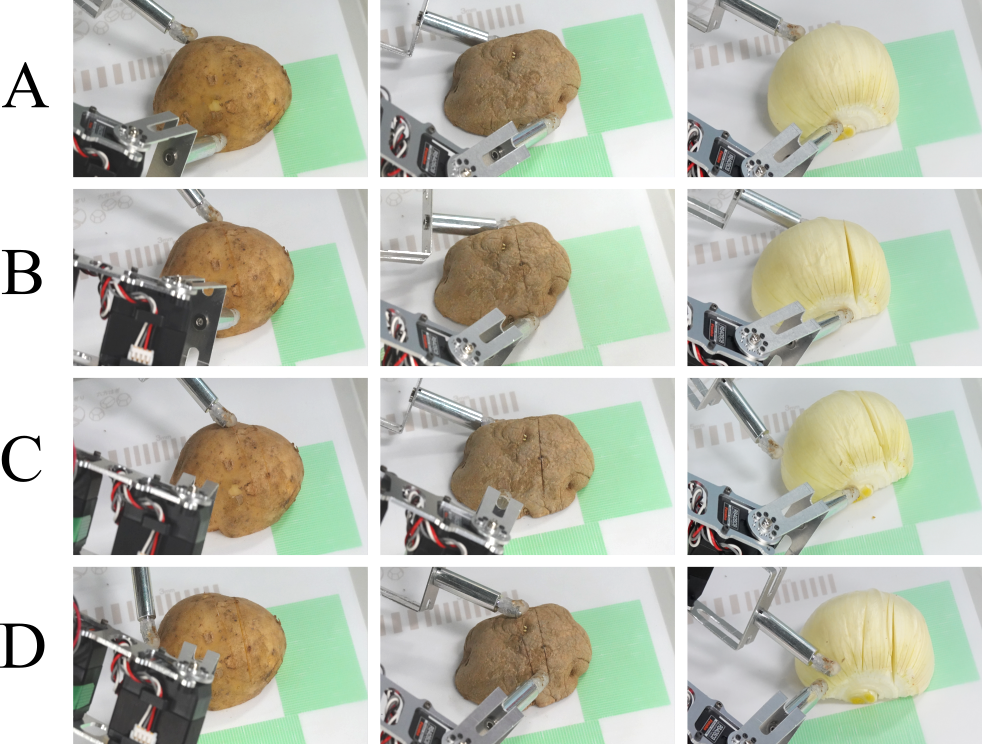
\includegraphics[width=0.85\linewidth]{fig/chp_holding/ICRA2024_HoldingExp.png}
    \caption{Images of the food-stuffs cut by each type of method (in the row).}
    \label{fig:holding_exp_holding_points_type}
\end{figure}

実ロボットによる切断実験では，6個の半切りジャガイモと4個の半切り玉ねぎを対象とし，提案手法（手法A）を含む4種類の把持点選択手法の安定性を比較した．

手法BおよびCは，幾何フィルタ後の上位60\%候補の中から，それぞれ中位および最低位の評価スコアを持つ{\nameholdingpointset}を選択する条件である．手法Dは，幾何フィルタ適用前の全候補$\equsearchspace_{\mathrm{all}}$からランダムに選択する条件である．

各食材は4手法で1回ずつ切断され，切断前後に固定カメラで撮影した画像から食材の平行移動量（pixel）と回転量（deg）を計測することで把持安定性を評価した．なお，同一食材に対する繰り返し切断による切断力の低下を防ぐため，各切断後に計画切断面をその法線方向に2mmずつ移動させた．

実験に用いた食材の物理パラメータは，Muら\cite{method-cutting-fracture}の手法により測定した値を使用した．ジャガイモの破壊靭性は409.66\,J/m$^2$，圧力分布は3352.07\,N/m$^2$，玉ねぎの破壊靭性は646.46\,J/m$^2$，圧力分布は3971.2\,N/m$^2$である．評価関数の重みは，$w_{\mathrm{fin}}=1,\ w_{\mathrm{knf}}=4.4,\ w_{\mathrm{tbl}}=6$，$w_{\mathrm{pdir}}=5,\ w_{\mathrm{pdis}}=4$，$w_{\mathrm{dir}}=2,\ w_{\mathrm{mag}}=2,\ w_{\mathrm{var}}=1$とした．

\begin{table}[H]
\centering
\setlength{\tabcolsep}{3pt}
\caption{Translation (in pixel) \& rotation (in degree) after cutting. The potato cut 6 times, onion cut 4 times.}
\label{tab:holding_exp_result}
\begin{tabular}{ccccccccccc}
\hline
\multirow{2}{*}{\begin{tabular}[c]{@{}c@{}}Holding\\ Type\end{tabular}} &
  \multirow{2}{*}{Food} &
  \multirow{2}{*}{\begin{tabular}[c]{@{}c@{}}Data\\ Type\end{tabular}} &
  \multirow{2}{*}{Avg.} &
  \multirow{2}{*}{Std.} &
  \multicolumn{6}{c}{Oringin Data} \\ \cline{6-11} 
                   &                         &                        &        &                             & 1      & 2      & 3      & 4      & 5      & 6      \\ \hline
\multirow{4}{*}{A} & \multirow{2}{*}{Potato} & \multicolumn{1}{c|}{T} & 113.85 & \multicolumn{1}{c|}{93.13}  & 259.40 & 47.00  & 197.70 & 61.50  & 28.20  & 89.30  \\
                   &                         & \multicolumn{1}{c|}{R} & 3.48   & \multicolumn{1}{c|}{4.30}   & 0.00   & 0.00   & 3.53   & 0.00   & 7.65   & 9.70   \\ \cline{4-11} 
                   & \multirow{2}{*}{Onion}  & \multicolumn{1}{c|}{T} & 84.45  & \multicolumn{1}{c|}{117.06} & 14.40  & 14.80  & 50.40  & 258.20 & ---    & ---    \\
                   &                         & \multicolumn{1}{c|}{R} & 0.99   & \multicolumn{1}{c|}{1.99}   & 0.00   & 0.00   & 0.00   & 3.97   & ---    & ---    \\ \hline
\multirow{4}{*}{B} & \multirow{2}{*}{Potato} & \multicolumn{1}{c|}{T} & 230.03 & \multicolumn{1}{c|}{290.15} & 646.00 & 24.00  & 12.30  & 36.70  & 106.50 & 554.70 \\
                   &                         & \multicolumn{1}{c|}{R} & 5.28   & \multicolumn{1}{c|}{6.36}   & 13.12  & 0.00   & 0.00   & 0.00   & 5.73   & 12.84  \\ \cline{2-11} 
                   & \multirow{2}{*}{Onion}  & \multicolumn{1}{c|}{T} & 41.03  & \multicolumn{1}{c|}{16.49}  & 48.50  & 35.30  & 59.20  & 21.10  & ---    & ---    \\
                   &                         & \multicolumn{1}{c|}{R} & 0.00   & \multicolumn{1}{c|}{0.00}   & 0.00   & 0.00   & 0.00   & 0.00   & ---    & ---    \\ \hline
\multirow{4}{*}{C} & \multirow{2}{*}{Potato} & \multicolumn{1}{c|}{T} & 165.07 & \multicolumn{1}{c|}{191.30} & 526.20 & 76.40  & 114.50 & 21.70  & 222.00 & 29.60  \\
                   &                         & \multicolumn{1}{c|}{R} & 3.85   & \multicolumn{1}{c|}{5.54}   & 14.50  & 0.00   & 2.14   & 5.06   & 1.40   & 0.00   \\ \cline{2-11} 
                   & \multirow{2}{*}{Onion}  & \multicolumn{1}{c|}{T} & 142.90 & \multicolumn{1}{c|}{109.59} & 289.80 & 145.90 & 108.00 & 27.90  & ---    & ---    \\
                   &                         & \multicolumn{1}{c|}{R} & 4.01   & \multicolumn{1}{c|}{5.16}   & 11.45  & 3.43   & 1.15   & 0.00   & ---    & ---    \\ \hline\hline
\multirow{4}{*}{D} & \multirow{2}{*}{Potato} & \multicolumn{1}{c|}{T} & 407.50 & \multicolumn{1}{c|}{198.05} & 759.50 & 304.70 & 263.70 & 520.30 & 345.50 & 251.30 \\
                   &                         & \multicolumn{1}{c|}{R} & 7.69   & \multicolumn{1}{c|}{7.31}   & 16.92  & 1.62   & 3.34   & 8.39   & 15.87  & 0.00   \\ \cline{2-11} 
                   & \multirow{2}{*}{Onion}  & \multicolumn{1}{c|}{T} & 429.70 & \multicolumn{1}{c|}{202.56} & 160.40 & 403.30 & 633.00 & 522.10 & ---    & ---    \\
                   &                         & \multicolumn{1}{c|}{R} & 6.22   & \multicolumn{1}{c|}{3.38}   & 1.28   & 7.25   & 7.39   & 8.96   & ---    & ---    \\ \hline
\end{tabular}
\end{table}

実験結果を表\ref{tab:holding_exp_result}に示す．手法AおよびBは手法CおよびDと比較して明らかに小さな移動量を示し，評価スコアの高い{\nameholdingpointset}ほど安定した把持が実現できることが確認された．

一方で，手法AとBの間には有意な差が見られなかった．これは，幾何フィルタ段階で明らかに不適切な候補が既に排除されており，上位候補はいずれも一定水準以上の安定性を有していたためと考察される．

また，手法AおよびBにおいても一部の試行で大きな移動量（外れ値）が観測されたが，その主因はRGB-Dカメラ点群に残留するノイズによる形状モデルの誤差，およびサーボのPID制御における不感帯に起因する{\namefingerpoint}決め誤差（最大約1cm）であると特定された．

さらに，本実験の評価法そのものにも限界がある．切断前後の画像比較のみでは切断途中の安定性を直接評価できず，往復スライス動作によって切断終了時に食材が元の位置近くに戻された場合，実際には途中で大きく移動していても変位が小さく評価される可能性がある．切断過程全体を通した把持安定性の評価は今後の課題である．


\subsection{完全切断による実用性の実証}
\label{subsec:holding_exp_complete_cut}

\begin{figure}[t]
    \centering
    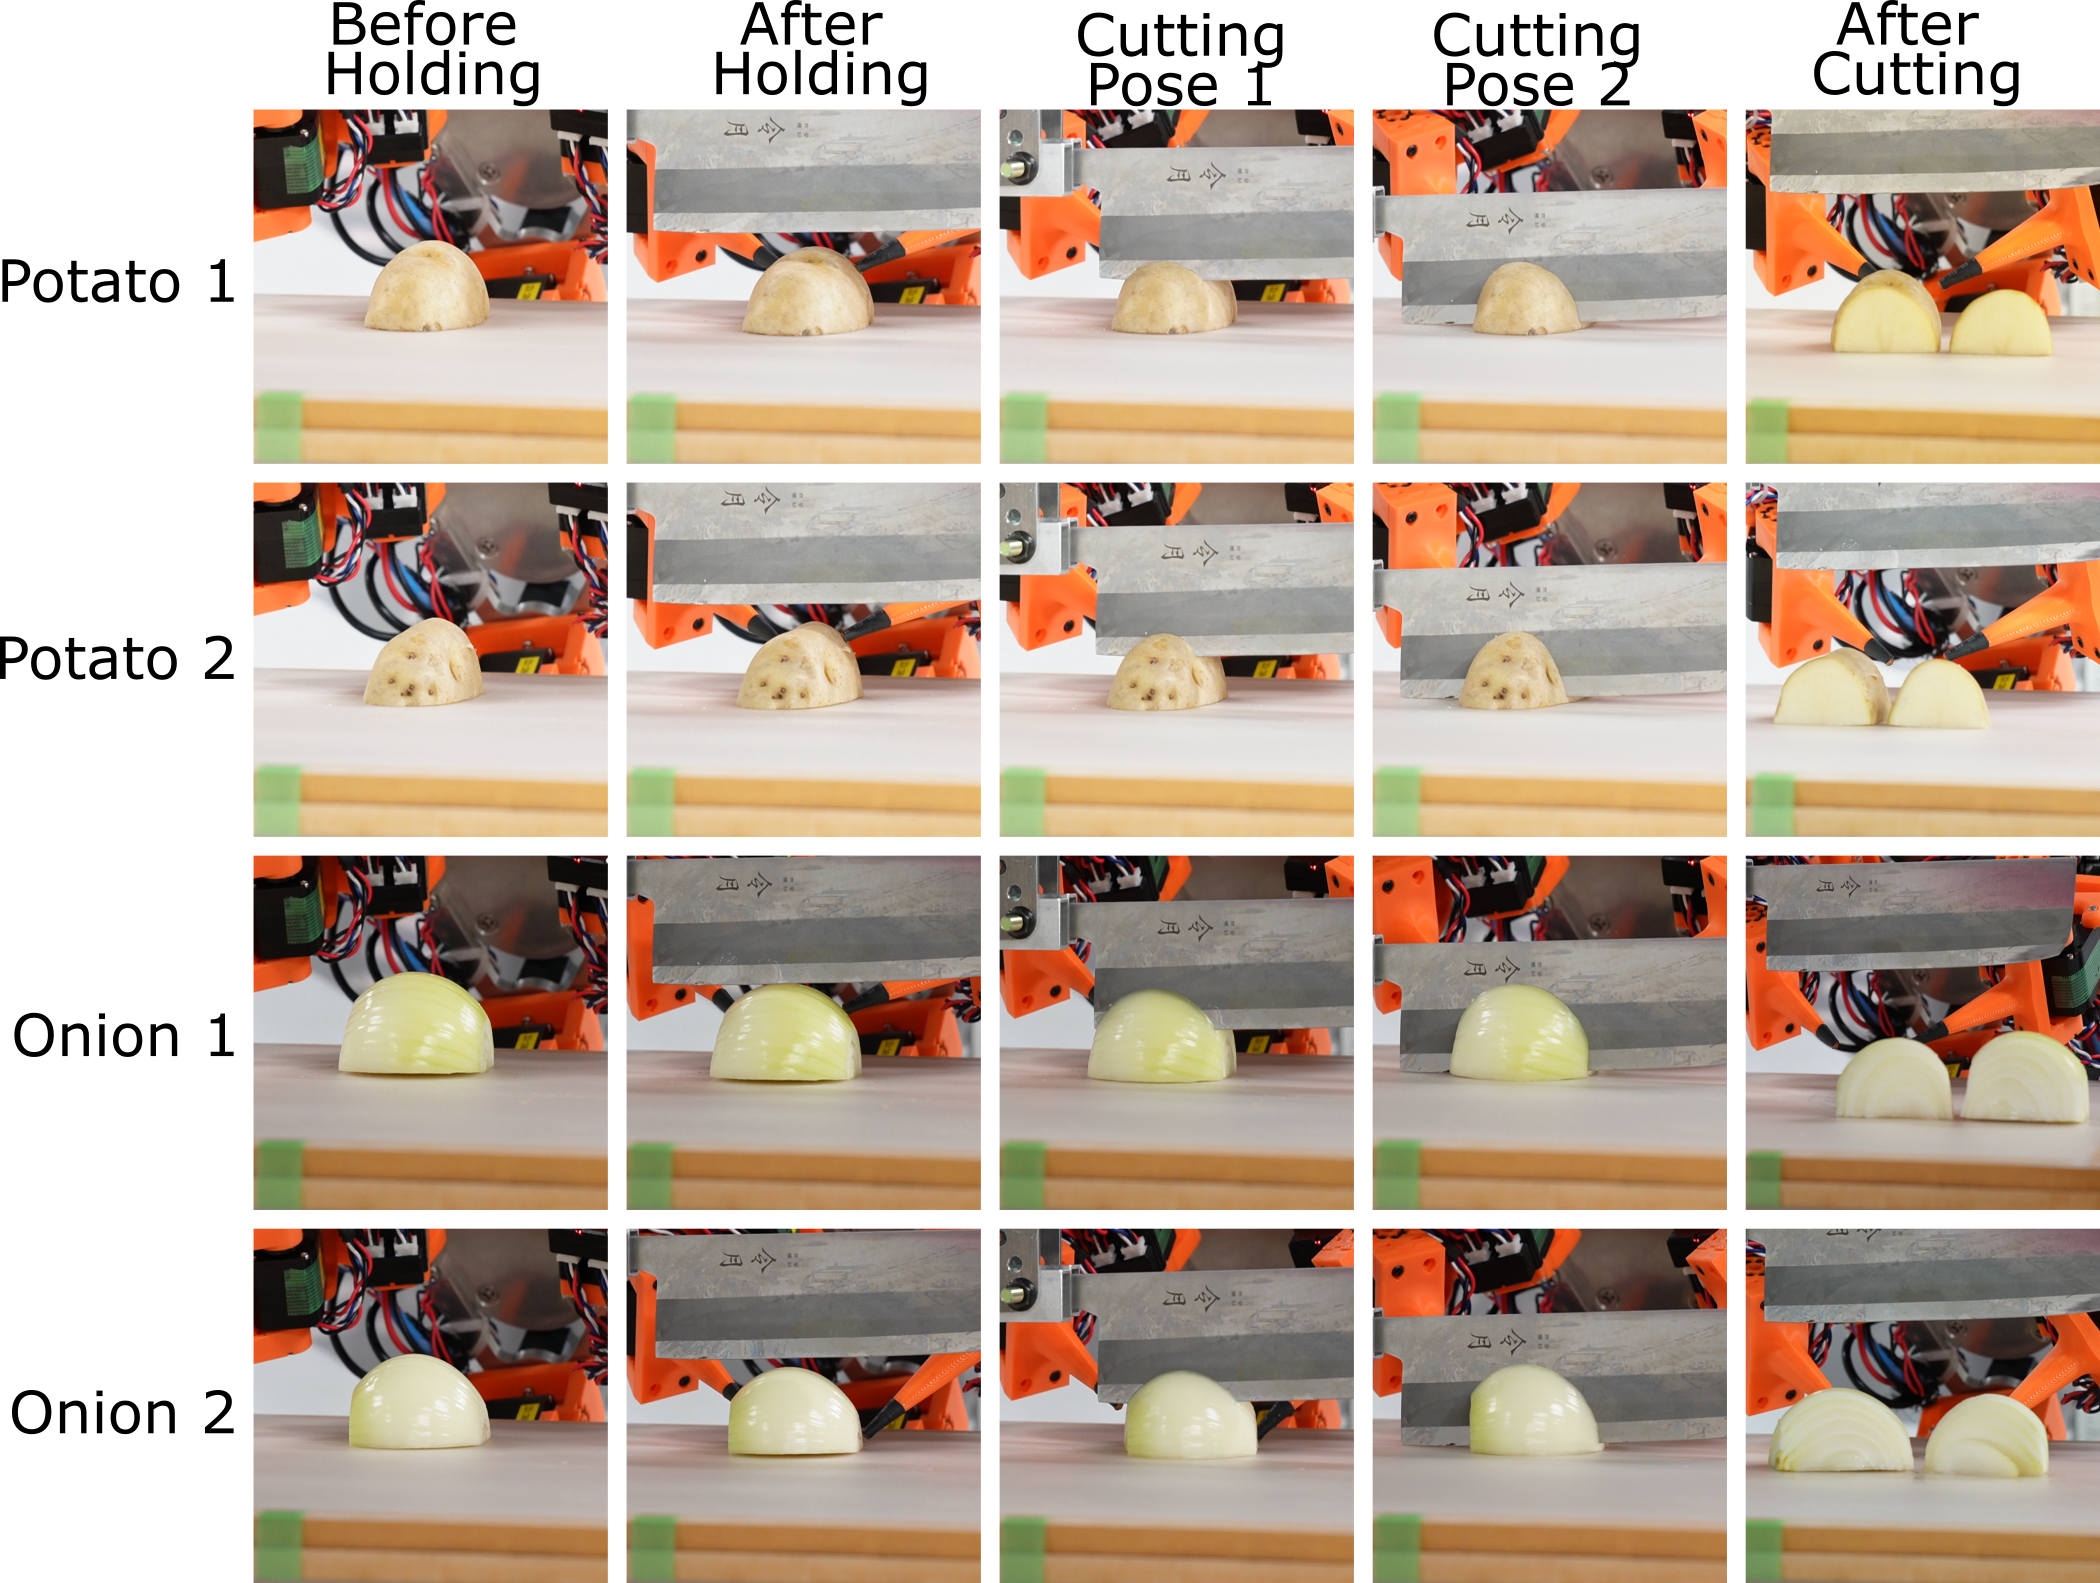
\includegraphics[width=0.95\linewidth]{fig/chp_holding/exp_full_cutting.png}
    \caption{\fix[Snapshots of the cutting process. The rows correspond to different experimental trials with potatoes and onions, while the columns depict the sequential stages of the task (from 'Before Holding' to 'After Cutting').]}
    \label{fig:holding_exp_full_cutting}
\end{figure}

比較実験がサンプル形状保存のための部分切断にとどまるのに対し，本節では食材を完全に切断する実験を行い，提案手法の実用性を検証した．

図\ref{fig:holding_exp_full_cutting}に示す通り，提案手法により選定された{\nameholdingpointset}は，ジャガイモ・玉ねぎのいずれにおいても完全切断の全工程を通じて安定性を維持し，断面の滑らかな切断面が得られた．

\revise{切断中に観測された変位は1\,cm未満であり，把持点での滑りよりもサーボハンドの機械的剛性限界による変形が主因であった．この結果は，平坦面を持つ半切り食材，既知の物性値および包丁軌道という条件下で，食材の大きな移動を防ぎ，滑らかな切断面を伴う完全切断を実行できたことを示す．家庭の食材一般に対する十分性を意味するものではない．}


\subsection{計算コスト分析と実応用に向けた考察}
\label{subsec:holding_exp_computation}

% \begin{table}[H]
%   \centering
%   \caption{\fix[Computation time and score at different point counts.]}
%   % 使用 resizebox 自动缩放表格以适应页面宽度
%   \resizebox{\linewidth}{!}{%
%   \fix[
%   \begin{tabular}{lccccccccc}
%     \toprule
%     \textbf{Point Count} & 7 & 11 & 22 & 62 & 114 & \textbf{169} & 356 & 668 & 1220 \\
%     \midrule
%     \textbf{Time (s)}    & 3.3 & 3.7 & 6.9 & 12.9 & 32.8 & \textbf{75.4} & 283.0 & 995.0 & 3297.7 \\
%     \textbf{Best Score}  & -- & -- & 20.31 & 22.19 & 22.19 & \textbf{22.85} & 22.89 & 22.74 & 22.82 \\
%     \bottomrule
%   \end{tabular}%
% ]
%   % }
% \end{table}
\begin{table}[t]
  \centering
  \caption{\fix[Computation time and score at different point counts.]}
  % 使用 resizebox 自动缩放表格以适应页面宽度
  \label{tab:holding_sensitivity_analysis}
  % \resizebox{\linewidth}{!}
  % {%
  \fix[
  \begin{tabular}{lccccccccc}
    \toprule
    \textbf{Point Count} & 7 & 11 & 22 & 62 & 114 & \textbf{169} & 356 & 668 & 1220 \\
    \midrule
    \textbf{Time (s)}    & 3.3 & 3.7 & 6.9 & 12.9 & 32.8 & \textbf{75.4} & 283.0 & 995.0 & 3297.7 \\
    \textbf{Best Score}  & -- & -- & 20.31 & 22.19 & 22.19 & \textbf{22.85} & 22.89 & 22.74 & 22.82 \\
    \bottomrule
  \end{tabular}%
]
  % }
\end{table}

提案手法の実用展開を見据え，点群密度を7点から1220点まで変化させた際の計算時間と評価スコアの関係を分析した．全計算は，AMD Ryzen 9 3900X 12-Core Processor，64GB RAMを搭載した標準的なPC上で実行した．

実験に採用した約170点の点群密度では平均計算時間は75.4秒であり，評価スコアは約22.85で増加しにくいことが確認された（表\ref{tab:holding_sensitivity_analysis}）．これ以上の点群密度増加はスコア改善にほとんど寄与せず，計算時間のみを増大させる．

\begin{revisionblock}
計算時間の大部分は動的評価スコアの計算（アルゴリズム\ref{algo:holding_filter_force}のCalDynamicScore）が占めており，これは多数の{\namegraspforce}候補を生成・評価する処理に起因する．
現状の実装はオフライン計画を前提とし，約170点でも平均75.4秒を要する．
この待ち時間を家庭内で許容できるかは，並行して行える準備作業や料理工程全体の所要時間に依存するため，本実験だけから十分に許容可能とは結論しない．
力評価処理の並列化，候補点の適応的削減，および再計画頻度の検討が必要である．
\end{revisionblock}

\begin{revisionblock}
\subsection{家庭内の切断作業としての評価}
家庭料理の観点で本章の中心的な成果は，評価スコアそのものではなく，選定した把持点に指を配置することで，半切りのジャガイモと玉ねぎが包丁外力を受けても大きく移動せず，最後まで切断できたことである．
比較実験では，高スコア候補が低スコア・ランダム候補より移動を抑える傾向を示し，完全切断実験では変位を1\,cm未満に保って滑らかな切断面を得た．
この結果により，食材形状を単に認識するだけでなく，既知の切断条件と組み合わせて調理目的に対応する接触位置を決められることを示した．

一方，対象は平坦面を持つ半切り食材二種類であり，丸い食材，柔軟・脆弱な食材，物性が未知の食材には直接適用できない．
包丁軌道と物性値を事前に与える必要があり，計画に約75秒を要し，切断中の変位評価も前後画像を中心としている．
また，指と刃の安全距離は幾何フィルタで扱うが，人共存下の安全，食品衛生，刃物の洗浄は評価していない．
したがって，本章の達成範囲は，設定した食材・接触・物性条件下での安定把持点選択と完全切断である．
\end{revisionblock}


% % ------------------------------------------------------------
% \section{本章のまとめ}
% \label{sec:holding_summary}
% % ------------------------------------------------------------

% 本章では，包丁による食材切断時に生じる外力に対し，食材の意図しない移動を防ぐための{\nameholdingpointset}探索手法を提案した．

% 提案手法の核心は，幾何フィルタによる{\namesearchspace}の効率的削減，包丁が食材に与える力とトルクの力学的推定，{\namegraspforce}の冗長性を考慮した効率的な力候補生成，および大きさ・方向・分散の三基準に基づく動的評価スコアの統合にある．

% 双腕ロボットシステムを用いた実機実験により，提案手法がランダム選択や低スコア候補と比較して有意に高い把持安定性を達成することが示された．さらに完全切断実験により，実用的な切断タスクへの適用可能性も確認された．

% 一方で，現状の手法には平坦な底面を前提とした運動制約，切断前後の画像比較に依存した評価法，および計算時間の制約という限界が残されている．底面が平坦でない食材や球状食材への拡張，切断過程全体を通した把持安定性の評価，および計算の高速化は今後の課題である．



% ------------------------------------------------------------
\section{本章のまとめ}
\label{sec:holding_summary}
% ------------------------------------------------------------

\revise{本章では，食材点群，既知の包丁軌道，指本数，および既知・計測済みの物性値を入力とし，切断中の時間変化するWrenchに抗する{\nameholdingpointset}と指先力を出力するタスク固有の探索手法を構築し，実機で検証した．}
具体的には，以下の分析と制御の流れによって，切断軌道全体にわたる安定把持を実現した．

\begin{enumerate}
	\item \textbf{幾何学的な分析：} RGB-Dカメラで取得した食材の離散点群モデルを用いて{\nameholdingpointset}候補を生成し，指同士の距離・指と包丁の距離・指の高さからなる幾何フィルタによって{\namesearchspace}を効率的に削減した．さらに，{\nameholdingpointset}の主成分方向と包丁平面法線の関係，および各{\namefingerpoint}から包丁平面までの距離を評価する位置評価スコアを設計し，外力に抵抗しやすい幾何配置を優先する仕組みを導入した．
	\item \textbf{力学的な分析：} 食材の破壊靭性と包丁速度に基づき，切断力と摩擦力を統合した時間変化する包丁外力を推定した．また，{\namegraspforce}の冗長性を考慮し，摩擦円錐内に{\namefingerforce}を限定した効率的な力候補生成手法を提案するとともに，{\namefingerforce}の大きさ・方向・分散の三基準による動的評価スコアを局所・大域の二段階で算出し，力学的に最も安定な{\nameholdingpointset}を選出した．
	\item \textbf{動作制御：} 分析により選定された{\nameholdingpointset}$P_{\mathrm{fin}}$に基づき，双腕ロボットの左腕指ハンドを逆運動学により各接触点へ誘導し把持を実行した．その後，右腕に固定した包丁を，分析時に力学的評価の前提として参照した往復スライス軌道に沿って動作させ，分析から制御まで一貫した切断タスクの遂行を可能とした．
\end{enumerate}

実機による検証として，以下の実験を実施し，提案手法の有効性を確認した．
\begin{enumerate}
	\item \textbf{{\namegraspforce}候補の生成効率評価：} 提案する力候補生成手法は，従来のランダム$\bm{k}$法の約4.2\%の成功率に対し，平均32.3\%の成功率を達成し，約7.7倍の効率的な生成を実現した．
	\item \textbf{把持安定性の比較実験：} ジャガイモおよびタマネギを対象に，提案手法（最高スコア）と中位・低スコア・ランダム選択の4条件で比較切断実験を行い，提案手法が高スコア候補は低スコア・ランダム候補に比べて安定する傾向を示したことを確認した．
	\item \textbf{完全切断実験：} 実際に食材を最後まで切断する実験を通じ，提案手法により選定された{\nameholdingpointset}が全工程を通じて安定性を維持し，滑らかな切断面が得られることを実証した．
	\item \textbf{計算コストの分析：} 点群密度と計算時間・評価スコアの関係を調査し，約170点の点群でスコアが飽和し，平均計算時間は約75秒であることを示した．\revise{この時間はオンライン再計画には長く，家庭内での許容性は料理工程全体との関係で別途評価する必要がある．}
\end{enumerate}

一方で，本手法は食材の平坦な底面を前提とした運動制約に依存しており，非平坦な底面への拡張が今後の課題である．
計算の高速化についても，力学的な分析の部分のGPU並列化などによるリアルタイム化が実用化に向けた重要な課題として残されている．
\revise{以上より，幾何情報を候補削減に用い，さらに包丁軌道に沿う力学評価を加えることで，設定条件下では食材移動を抑えて完全切断できる把持点を選定可能になった．ただし，この結論は物性値，包丁軌道，平面接触が与えられる範囲に限定される．}

	\chapter{結言}
\label{chap:conclusion}

\section{本論文の総括}
\label{sec:conclusion_overview}

\begin{revisionblock}
本論文は，家庭用料理ロボットのうち，操作目的，使用する道具の基本機能，および作業条件が与えられた後の操作実行層を対象とした．
食材・容器・道具の個体差に対し，形状，力学，環境・道具の拘束という観点から必要な量を整理し，RGB-D点群と既知または計測可能な物理条件から，軌道，操作量，把持位置，力・角度などの実行パラメータを導出する方法を検討した．
レシピ理解，献立・作業計画，食材や道具の選択，複数タスクの自律切替え，および料理工程全体の自動化は本論文の対象外である．
\end{revisionblock}
家庭の食材，容器，および調理器具は，形状，大きさ，材質，配置が一定ではなく，工場のような専用治具や固定環境を前提とできない．
この条件では，事前に与えた単一の軌道を再生するだけではなく，その場で取得した対象・環境モデルから，タスクの成立に必要な量を計算することが重要となる．

\begin{revisionblock}
本論文では，センシングによって得た3Dモデルを認識処理の終点とせず，タスク固有の分析と動作設計の入力として用いた．
具体的には，3D点群から表面位置，法線，断面積，体積，重心を抽出し，タスクに応じて軌道，目標角度，{\nameholdingpointset}，および制御パラメータへ変換した．
ただし，「センシング，モデリング，分析，動作計画・制御」という流れ自体は一般的であり，本論文はこれを単一の新規アルゴリズムまたは三タスク共通の解法として提案するものではない．
皮むきでは表面法線・既処理境界・接触力，注ぎでは容器形状と液面または傾斜角度，安定把持では切断Wrench・摩擦・力の釣合いという異なる関係を構成した点に，各タスクの技術的特徴がある．
\end{revisionblock}

\revise{共通の分析観点を異なる物理的相互作用へ適用し，タスク固有手法として具体化できる範囲を検証するため，本論文では，皮むき，定量注ぎ，および切断中の安定把持を取り上げた．}
皮むき作業では不規則曲面への幾何学的適応，注ぎでは容器を介した流体の間接操作，切断中の把持では包丁外力に抵抗する力学的な安定性を扱った．
\revise{三つのタスクは，料理工程の網羅率を示すためではなく，形状，力学，環境・道具の拘束の組合せが相補的になるように選定した．対象となる物理現象と3Dモデルの利用法は異なるが，支配条件を明示し，計測可能な量を実行パラメータへ接続するという分析観点を共有する．}

\section{各研究課題で得られた成果}
\label{sec:conclusion_results}

\subsection{システム構成と3Dモデルの取得}
\label{subsec:conclusion_common_model}

第\ref{ch:system}章では，三つのタスクに共通する計測・実装基盤を構築した．PA10-7Cを用いた双腕システムとDENSO VS-050を用いた双腕システムについて，ロボット，RGB-Dカメラ，力覚センサ，グリッパ，エンドエフェクタ，およびソフトウェア構成を整理した．

\revise{標準物体および3Dプリンタ製曲面物体による評価では，円柱標準物体に対して全条件平均で半径誤差が $-0.716 \pm 0.175~\mathrm{mm}$ となり，位置誤差もおおむね $1$--$2~\mathrm{mm}$ 程度に収まることを確認した．}
また，3Dプリンタ製容器に対しては，点群モデルから平均相対誤差 $2.31\%$ で容積を推定でき，CADモデルに対する表面形状のRMSEは $1.424$--$3.522~\mathrm{mm}$ であった．
\revise{さらに，卓上観測では原理的に欠落する底面側について，対象を把持して持ち上げ，能動的に提示姿勢を変えて再撮影することで補完した．底面点群を含むモデルのRMSEは $5.715$--$6.789~\mathrm{mm}$であり誤差増加を伴うが，卓上スキャンだけでは得られない不規則物体の下面情報を把持候補生成へ供給できた．}

以上により，後続する各タスクへ，位置・姿勢，色，法線，断面積，体積，重心を受け渡す共通の基盤を構築した．

\subsection{タスク1：皮むき作業}
\label{subsec:conclusion_peeling}

第\ref{ch:peeling}章では，第\ref{ch:introduction}章で設定した第一の検証である皮むき動作を扱った．
食材表面点群と作業台・到達可能領域の幾何関係からピーラーの基準軌跡を抽出し，表面法線の変化に基づいて軌跡を複数の実行区間へ分割した．
さらに，非皮領域の色と境界近傍の法線から食材の回転角を計算し，「一回皮むき動作」と「食材の回転操作」を反復する作業構成を実現した．

実行時には，点群モデルから得た軌跡を位置制御の基準とし，ピーラーと食材の接触力を力覚フィードバックで維持した．
これにより，点群の局所誤差，食材表面の凹凸，および刃先の実際の切込み位置とモデル表面との差を実行時情報で補償した．

実験について，りんご，きゅうり，なす，じゃがいも，にんじんを利用して13回の皮むきでは，全ての対象で78\%以上の皮むき率を得た．
この結果は，本実験で扱った対象と条件において，3D表面幾何から生成した動作と接触力制御の組合せが，不規則形状へ適応する皮むきに有効であることを示す．

\subsection{タスク2：液体注ぐ作業}
\label{subsec:conclusion_pouring}

第\ref{ch:pour}章では，直接把持できない液体を，容器という環境を介して操作する定量注ぎを扱った．
手法1では，注ぎ先容器の3Dモデルと実行中に検出した液面高さから注いだ体積を推定し，体積誤差を用いたPD制御により注ぐ容器の角速度を調整した．
手法2では，注ぐ容器の3Dモデルから注ぎ縁と注ぐポイントを検出し，容器角度と注いだ体積の関係を事前計算した上で，目標体積に対応する角度へP制御で追跡した．

形状特性の異なる三種類の容器を用いた実験により，注ぎ先容器を基準とする手法1では，容器3において平均誤差$-0.95$~ml，標準偏差1.16~mlを得た．
注ぐ容器を基準とする手法2では，同容器において平均誤差4.96~ml，標準偏差2.57~mlとなった．
手法1は実行中の液面観測を必要とする一方で高い精度を示し，手法2は液面を観測できない場合でも実行できる一方で，表面張力，容器壁厚，および初期液体量の誤差の影響を受けた．

この結果は，液体の流体モデルを直接構築しなくても，液体を拘束する容器の幾何を計算代理として用いることで，注いだ体積と制御目標を導出できることを示す．
ただし，手法1は液面が観測できること，手法2は注ぐ容器の形状と初期液体の量が得られることを必要とし，低粘度液体，凸形状に基づく断面計算，および表面張力を無視した近似などの仮定を含む．

\subsection{タスク3：切断時の安定把持}
\label{subsec:conclusion_holding}

第\ref{ch:holding}章では，第\ref{ch:introduction}章で設定した第三の検証として，包丁から加わる外力に抵抗しながら食材を安定に把持できる{\nameholdingpointset}探索を扱った．
食材表面点群と包丁軌道を入力とし，まず包丁・作業台・指間の幾何的なフィルタを用いて探索空間を削減した．
次に，包丁刃と食材の接触から切断力を推定し，その外力を釣り合える把持力の候補を生成した．
さらに，把持力の大きさ，方向，および指間分散に基づく動的評価を包丁軌道全体で累積し，最終{\nameholdingpointset}を選定した．

ジャガイモと玉ねぎを用いた比較実験では，高い評価スコアを持つ{\nameholdingpointset}は，ランダム候補および低スコア候補と比べて切断前後の移動量が小さい傾向を示した．また，選定した{\nameholdingpointset}を用いた完全切断を実機で実行し，対象を保持したまま切断工程を完了できることを確認した．これにより，3D形状だけでなく，包丁軌道に沿って変化する外力と道具拘束をモデル上で評価することが，{\nameholdingpointset}の選定に有効であることを示した．

一方で，本手法は食材の平坦な底面を前提とした運動制約に依存しており，非平坦な底面への拡張が今後の課題である．
計算の高速化についても，力学的な分析の部分のGPU並列化などによるリアルタイム化が実用化に向けた重要な課題として残されている．

\begin{revisionblock}
\section{本論文により可能となったことと適用範囲}
\label{sec:conclusion_scope}

本論文によって，事前に精密なCADモデルを登録して対象ごとの軌道・把持点を教示する代わりに，設定した条件下では，その場で得た個体形状を次の実行量へ変換することが可能となった．

\begin{enumerate}
  \item 皮むきでは，個体食材の表面形状からピーラーの到達可能軌道と食材回転量を生成し，点群誤差と表面凹凸を力覚で補償できる．
  \item 注ぎでは，事前登録していない容器形状から液面高さ・体積関係または傾斜角度・流出量関係を求め，制御時に補助計量器を用いず指定量に対応する制御目標を生成できる．
  \item 安定把持では，食材形状だけでなく，包丁軌道に沿って時間変化する切断力・モーメントと接触条件を評価し，食材移動を抑えて完全切断できる把持点を選択できる．
  \item 計測面では，卓上から不可視となる不規則物体の下面を，ロボットによる持ち上げと再撮影で能動的に取得し，元の姿勢へ統合できる．
\end{enumerate}

この適用範囲は，料理工程上の範囲と物理的相互作用上の範囲を分けて解釈する必要がある．
料理工程上，本論文が扱うのは下処理・材料操作に含まれる三つの個別操作であり，レシピ理解，加熱制御，味付け判断，盛付け，洗浄，工程間の計画を含まない．
したがって，料理全体に対する数値的な網羅率は主張しない．
一方，物理的相互作用上は，不規則固体表面への道具接触，容器を介した低粘性流体の定量移送，大きな外力に抗する多点接触という異なる組合せを扱い，三つの分析観点を相補的に検証した．

他の料理操作へ展開するためには，（i）操作目的と道具の役割が定義されていること，（ii）支配条件を形状，力学，環境・道具の拘束として記述できること，（iii）必要な量を3Dモデルと既知または計測可能な物理条件から計算できること，（iv）結果を軌道，操作量，把持位置，力・角度などの実行パラメータへ変換できること，が必要である．
これらを満たさないタスクに三つの既存アルゴリズムをそのまま適用できるとは限らず，新たなタスク固有モデルと検証が必要である．
\end{revisionblock}


\section{今後の展望}
\label{sec:conclusion_future}

今後の第1の課題は，3Dモデル取得のロバスト化と不確実性の明示である．
複数センサ，偏光・熱・近接・触覚情報，および物体を動かしながら観測する能動知覚を組み合わせ，透明・反射・遮蔽領域を補完する必要がある．
また，点群の各領域に位置・法線・体積推定の信頼度を付与し，信頼度が低い場合に再観測を行う仕組みが有効である．

第2の課題は，計算と実行の高速化である．特に切断中把持では，把持力候補の生成と評価が計算時間の大部分を占める．候補生成の階層化，GPU並列化，近似最適化，および過去タスクからの初期解再利用により，環境変化へ応答可能な計画速度を目指す必要がある．

\begin{revisionblock}
より長期的な目標は，これらの操作実行技術を，家庭内で一連の料理を支援するロボットへ統合することである．
本論文の双腕実験装置は計測と手法検証を目的としており，寸法，設置空間，処理時間，安全・衛生の点で，そのまま一般家庭へ導入できるものではない．
一方，小型の双腕機構や人型ロボットのハードウェア，レシピ・作業計画，物体認識，安全制御の研究は進展している．
将来，それらの小型ハードウェアと上位計画機能に，本論文で示した個体形状に応じる皮むき，定量注ぎ，切断中把持の操作実行法を組み合わせることで，専用大型設備を必要としない家庭用料理ロボットへ段階的に近づけると考える．
その際には，三手法を単に並べるのではなく，上位層が各操作の目的・道具・許容誤差を与え，実行層が観測信頼度と物理条件に応じて再計測，従来器具の利用，または人への引継ぎを選択する統合が必要である．
\end{revisionblock}



	\chapter*{謝辞}
\addcontentsline{toc}{chapter}{謝辞}

本論文をまとめるにあたり，研究課題の設定から論文全体の構成，および研究者としての姿勢に至るまで，長期にわたり丁寧な指導をいただいた主任指導教員の工藤俊亮教授に深く感謝する．
研究の方向性に迷った際にも，多くの有意義な助言をいただき，本論文を一つの研究としてまとめることができた．

% TODO: 審査委員の氏名
本論文の審査にあたり，専門的な見地から有益な指摘と助言をいただいた審査委員の広田先生，木村先生，梶本先生，高橋先生，金森先生に厚く御礼を述べる．
いただいた指摘は，本研究の意義と限界を明確にし，論文の内容を改善する上で大きな助けとなった．

本研究の遂行において，共同研究，実験装置の構築，ソフトウェア開発，実験の実施，および日々の議論に協力いただいた研究室の教職員，卒業生，在学生の皆様に感謝する．
多くの技術的課題を解決できたのは，皆様から得た知識，助言，および協力によるものである．

また，長期間にわたる研究生活を理解し，支え続けてくれた家族と友人に心から感謝する．
研究が思うように進まない時期にも変わらず励ましてくれたことが，本論文を完成させる大きな力となった．

最後に，本研究に関わり，直接または間接に支援いただいた全ての方々へ，改めて深い感謝を表する．

    \bibliographystyle{junsrt}
	\bibliography{References}
    
    \chapter*{研究業績（関連論文）}
\addcontentsline{toc}{chapter}{研究業績（関連論文）}

\noindent\textbf{A. 学術論文}

\begin{enumerate}[
  label=\arabic*).,
  leftmargin=3em,
  itemsep=0.8\baselineskip
]
  \item Dong, C., Takizawa, M., Kimura, K., Suehiro, T., Kudoh, S. (2026). Searching method for holding points during robotic food cutting. SICE Journal of Control, Measurement, and System Integration, 19(1). 
  （第6章に関連）
\end{enumerate}

\vspace{1\baselineskip}
\noindent\textbf{B. 国際会議発表論文}

\begin{enumerate}[
  label=\arabic*).,
  leftmargin=3em,
  itemsep=0.8\baselineskip,
  resume
]
  \item C. Dong, L. Yu, M. Takizawa, S. Kudoh and T. Suehiro, "Food Peeling Method for Dual-arm Cooking Robot," 2021 IEEE/SICE International Symposium on System Integration (SII), Iwaki, Fukushima, Japan, 2021, pp. 801-806,
  （第4章に関連）

  \item C. Dong, M. Takizawa, S. Kudoh and T. Suehiro, "Precision Pouring into Unknown Containers by Service Robots," 2019 IEEE/RSJ International Conference on Intelligent Robots and Systems (IROS), Macau, China, 2019, pp. 5875-5882,
  （第5章に関連）
\end{enumerate}




\chapter*{研究業績（その他の論文）}
\addcontentsline{toc}{chapter}{研究業績（その他の論文）}
\vspace{1\baselineskip}

\noindent\textbf{A. 学術論文}

\begin{enumerate}[
  label=\arabic*).,
  leftmargin=3em,
  itemsep=0.8\baselineskip
]
  \item Hiroto Kitamori, Chenyu Dong, Masaru Takizawa, Shuya Watanabe, Jun Shintake, Kohei Kimura, and Shunsuke Kudoh. Origami manipulation by robot hand utilizing electroadhesion. ROBOMECH Journal, Vol. 11, No. 1, 9, 2024.
\end{enumerate}



\vspace{1\baselineskip}
\noindent\textbf{B. 国内会議発表論文}

\begin{enumerate}[
  label=\arabic*).,
  leftmargin=3em,
  itemsep=0.8\baselineskip
]
  \item 唐堅淇, 董晨宇, 上馬正寛, 木村航平, 工藤俊亮. ロボットアームを用いてカレーの具材を特定の比率で取り分ける手法の提案. 第25回計測自動制御学会システムインテグレーション部門講演会（SI2024）, 470-474, 2024.
  \item 上馬正寛, 董晨宇, 木村航平, 工藤俊亮. 料理ロボットによる野菜の乱切りのための切断手法の提案. 第42回日本ロボット学会学術講演会, 2I3-04, 2024.
  \item 鳥海真奈美, 上馬正寛, 董晨宇, 木村航平, 工藤俊亮. ロボットによる団子の丸め動作. ロボティクス・メカトロニクス講演会2024（ROBOMECH2024）, 2P2-F09, 2024.
  \item 北森洸人, 董晨宇, 滝澤優, 渡邉修也, 新竹純, 木村航平, 工藤俊亮. 電気接着を活用したロボットハンドによる折紙操作の実現. 第29回ロボティクスシンポジア, 3C4, 2024.
  \item 董晨宇, 滝澤優, 木村航平, 末廣尚士, 工藤俊亮. 食材切断のための食材把持方法の提案. 第41回日本ロボット学会学術講演会, 3E3-04, 2023.
  \item 劉雨晨, 董晨宇, 滝澤優, 末廣尚士, 工藤俊亮. ロボットアームによる巻き寿司具材のグラスピング. 第22回計測自動制御学会システムインテグレーション部門講演会（SI2021）, 817-820, 2021.
  \item 大蔵侑生, 董晨宇, 滝澤優, 末廣尚士, 工藤俊亮. 機械学習を用いた打音による容器内水量の推定. 第39回日本ロボット学会学術講演会, 2D3-04, 2021.
  \item 松井裕典, 董晨宇, 滝澤優, 末廣尚士, 工藤俊亮. ３種類の把持形態が可能な、指先に第２の挟持機構を備えたロボットハンド. 第39回日本ロボット学会学術講演会, 2B2-01, 2021.
  \item 見ル野雄大, 董晨宇, 滝澤優, 末廣尚士, 工藤俊亮. 深層学習によるバラ積みされたから揚げのピッキング. 第21回計測自動制御学会システムインテグレーション部門講演会（SI2020）, 2647-2651, 2020.
  \item 上野正汰, 滝澤優, 董晨宇, 末廣尚士, 工藤俊亮. 食材の特性に応じた食材集め動作の生成. 第38回日本ロボット学会学術講演会, 2K3-04, 2020.
  \item Li Ang, Dong Chenyu, 滝澤優, 工藤俊亮, 末廣尚士. 双腕ロボットによる食材の串刺し動作. 第37回日本ロボット学会学術講演会, 3E2-04, 2019.
  \item Dong ChenYu, 滝澤優, 工藤俊亮, 末廣尚士. ロボットによる液体の定量的な注ぎ作業の実現. 第36回日本ロボット学会学術講演会, 1A3-03, 2018.
\end{enumerate}
\end{document}
%--------------------------------------------------------------------
